\documentclass[10pt,compsoc,onecolumn]{IEEEtran}
\usepackage{etex}
\usepackage{etex}
\usepackage{amssymb,amsfonts,amsmath,amsthm}
\usepackage{graphicx}
 \usepackage[usenames,x11names, dvipsnames, svgnames]{xcolor}
\usepackage{amsmath,amssymb}
\usepackage{dsfont}
\usepackage{amsfonts}
\usepackage{mathrsfs}
\usepackage{hyperref}
\hypersetup{
    colorlinks=true,
    linkcolor=black,
    citecolor=MediumBlue,
    filecolor=black,
    urlcolor=DodgerBlue4,
    breaklinks=false,
%linkbordercolor=red,% hyperlink borders will be red
  %pdfborderstyle={/S/U/W 1}% border style will be underline of width 1pt
}
\usepackage{array}
%\usepackage{multirow}    
%\usepackage[T1,euler-digits]{eulervm}
%\usepackage{times}
%\usepackage{pxfonts}
\usepackage{tikz}
\usepackage{pgfplots}
\usetikzlibrary{shapes,calc,shadows,fadings,arrows,decorations.pathreplacing,automata,positioning}
\usetikzlibrary{external}
\usetikzlibrary{decorations.text}
\tikzexternalize[prefix=./Figures/External/]% activate externalization!
\tikzexternaldisable
%\addtolength{\voffset}{.1in}  
\usepackage{geometry}
\geometry{a4paper, left=.65in,right=.65in,top=.8in,bottom=0.8in}

\addtolength{\textwidth}{-.1in}    
\addtolength{\hoffset}{.05in}    
\addtolength{\textheight}{.1in}    
\addtolength{\footskip}{0in}    
\usepackage{rotating}
 \definecolor{nodecol}{RGB}{240,240,220}
 \definecolor{nodeedge}{RGB}{240,240,225}
  \definecolor{edgecol}{RGB}{130,130,130}
    \tikzset{%
fshadow/.style={      preaction={
         fill=black,opacity=.3,
         path fading=circle with fuzzy edge 20 percent,
         transform canvas={xshift=1mm,yshift=-1mm}
       }} 
}
\usetikzlibrary{pgfplots.dateplot}
 \usetikzlibrary{patterns}
\usetikzlibrary{decorations.markings}
\usepackage{fancyhdr}
\usepackage{mathtools}
\usepackage{datetime}
\usepackage{comment}
%% ## Equation Space Control---------------------------
\def\EQSP{4pt}
\newcommand{\mltlne}[2][\EQSP]{\begingroup\setlength\abovedisplayskip{#1}\setlength\belowdisplayskip{#1}\begin{equation}\begin{multlined} #2 \end{multlined}\end{equation}\endgroup}
\newcommand{\cgather}[2][\EQSP]{\begingroup\setlength\abovedisplayskip{#1}\setlength\belowdisplayskip{#1}\begin{gather} #2 \end{gather}\endgroup}
\newcommand{\cgathers}[2][\EQSP]{\begingroup\setlength\abovedisplayskip{#1}\setlength\belowdisplayskip{#1}\begin{gather*} #2 \end{gather*}\endgroup}
\newcommand{\calign}[2][\EQSP]{\begingroup\setlength\abovedisplayskip{#1}\setlength\belowdisplayskip{#1}\begin{align} #2 \end{align}\endgroup}
\newcommand{\caligns}[2][\EQSP]{\begingroup\setlength\abovedisplayskip{#1}\setlength\belowdisplayskip{#1}\begin{align*} #2 \end{align*}\endgroup}
\newcommand{\mnp}[2]{\begin{minipage}{#1}#2\end{minipage}} 
%% COLOR DEFS------------------------------------------
\newtheorem{thm}{Theorem}
\newtheorem{cor}{Corollary}
\newtheorem{lem}{Lemma}
\newtheorem{prop}{Proposition}
\newtheorem{defn}{Definition}
\newtheorem{example}{Example}
\newtheorem{rem}{Remark}
\newtheorem{notn}{Notation}
%%------------PROOF INCLUSION -----------------
\def\NOPROOF{Proof omitted.}
\newif\ifproof
\prooffalse % or \draftfalse
\newcommand{\Proof}[1]{
\ifproof
\begin{IEEEproof}
#1\end{IEEEproof}
\else
\NOPROOF
\fi
 }
%%------------ -----------------
\newcommand{\DETAILS}[1]{#1}
%%------------ -----------------
% color commands------------------------
\newcommand{\etal}{\textit{et} \mspace{3mu} \textit{al.}}
% \renewcommand{\algorithmiccomment}[1]{$/** $ #1 $ **/$}
\newcommand{\vect}[1]{\textbf{\textit{#1}}}
\newcommand{\figfont}{\fontsize{8}{8}\selectfont\strut}
\newcommand{\hlt}{ \bf \sffamily \itshape\color[rgb]{.1,.2,.45}}
\newcommand{\pitilde}{\widetilde{\pi}}
\newcommand{\Pitilde}{\widetilde{\Pi}}
\newcommand{\bvec}{\vartheta}
\newcommand{\algo}{\textrm{\bf\texttt{GenESeSS}}\xspace}
\newcommand{\xalgo}{\textrm{\bf\texttt{xGenESeSS}}\xspace}
\newcommand{\FNTST}{\bf }
\newcommand{\FNTED}{\color{darkgray} \scriptsize $\phantom{.}$}
\renewcommand{\baselinestretch}{.95}
\newcommand{\sync}{\otimes}
\newcommand{\psync}{\hspace{3pt}\overrightarrow{\hspace{-3pt}\sync}}
%\newcommand{\psync}{\raisebox{-4pt}{\begin{tikzpicture}\node[anchor=south] (A) {$\sync$};
%\draw [->,>=stealth] ([yshift=-2pt, xshift=2pt]A.north west) -- ([yshift=-2pt]A.north east); %\end{tikzpicture}}}
\newcommand{\base}[1]{\llbracket #1 \rrbracket}
\newcommand{\nst}{\textrm{\sffamily\textsc{Numstates}}}
\newcommand{\HA}{\boldsymbol{\mathds{H}}}
\newcommand{\eqp}{ \vartheta }
\newcommand{\entropy}[1]{\boldsymbol{h}\left ( #1 \right )}
\newcommand{\norm}[1]{\left\lVert #1 \right\rVert}%
\newcommand{\abs}[1]{\left\lvert #1 \right\rvert}%
\newcommand{\absB}[1]{\big\lvert #1 \big\rvert}%
% #############################################################
% #############################################################
% PREAMBLE ####################################################
% #############################################################
% #############################################################
% \usepackage{pnastwoF}
\DeclareMathOperator*{\argmax}{argmax}
\newcommand{\ND}{ \mathcal{N}  }
\usepackage[linesnumbered,ruled,vlined,noend]{algorithm2e}
\newcommand{\captionN}[1]{\caption{\color{darkgray} \sffamily \fontsize{8}{10}\selectfont #1  }}
\newcommand{\btl}{\ \textbf{\small\sffamily bits/letter}}
\usepackage{txfonts}
%\usepackage{ccfonts}
%%% save defaults
\renewcommand{\rmdefault}{phv} % Arial
\renewcommand{\sfdefault}{phv} % Arial
\edef\keptrmdefault{\rmdefault}
\edef\keptsfdefault{\sfdefault}
\edef\keptttdefault{\ttdefault}

%\usepackage{kerkis}
\usepackage[OT1]{fontenc}
%\usepackage{concmath}
\usepackage[T1]{eulervm}
%\usepackage[OT1]{fontenc}
%%% restore defaults
\edef\rmdefault{\keptrmdefault}
\edef\sfdefault{\keptsfdefault}
\edef\ttdefault{\keptttdefault}
\tikzexternalenable
% ##########################################################
\tikzfading[name=fade out,
            inner color=transparent!0,
            outer color=transparent!100]
%###################################
\newcommand{\xtitaut}[2]{
\noindent\mnp{\textwidth}{
\mnp{\textwidth}{\raggedright\Huge \bf \sffamily #1}

\vskip 1em

{\bf \sffamily #2}
}
\vskip 2em
}
%###################################
%###################################
\tikzset{wiggle/.style={decorate, decoration={random steps, amplitude=10pt}}}
\usetikzlibrary{decorations.pathmorphing}
\pgfdeclaredecoration{Snake}{initial}
{
  \state{initial}[switch if less than=+.625\pgfdecorationsegmentlength to final,
                  width=+.3125\pgfdecorationsegmentlength,
                  next state=down]{
    \pgfpathmoveto{\pgfqpoint{0pt}{\pgfdecorationsegmentamplitude}}
  }
  \state{down}[switch if less than=+.8125\pgfdecorationsegmentlength to end down,
               width=+.5\pgfdecorationsegmentlength,
               next state=up]{
    \pgfpathcosine{\pgfqpoint{.25\pgfdecorationsegmentlength}{-1\pgfdecorationsegmentamplitude}}
    \pgfpathsine{\pgfqpoint{.25\pgfdecorationsegmentlength}{-1\pgfdecorationsegmentamplitude}}
  }
  \state{up}[switch if less than=+.8125\pgfdecorationsegmentlength to end up,
             width=+.5\pgfdecorationsegmentlength,
             next state=down]{
    \pgfpathcosine{\pgfqpoint{.25\pgfdecorationsegmentlength}{\pgfdecorationsegmentamplitude}}
    \pgfpathsine{\pgfqpoint{.25\pgfdecorationsegmentlength}{\pgfdecorationsegmentamplitude}}
  }
  \state{end down}[width=+.3125\pgfdecorationsegmentlength,
                   next state=final]{
     \pgfpathcosine{\pgfqpoint{.15625\pgfdecorationsegmentlength}{-.5\pgfdecorationsegmentamplitude}}
     \pgfpathsine{\pgfqpoint{.15625\pgfdecorationsegmentlength}{-.5\pgfdecorationsegmentamplitude}}
  }
  \state{end up}[width=+.3125\pgfdecorationsegmentlength,
                 next state=final]{
     \pgfpathcosine{\pgfqpoint{.15625\pgfdecorationsegmentlength}{.5\pgfdecorationsegmentamplitude}}
     \pgfpathsine{\pgfqpoint{.15625\pgfdecorationsegmentlength}{.5\pgfdecorationsegmentamplitude}}
  }
  \state{final}{\pgfpathlineto{\pgfpointdecoratedpathlast}}
}
%###################################
%###################################
\newcolumntype{L}[1]{>{\rule{0pt}{2ex}\raggedright\let\newline\\\arraybackslash\hspace{0pt}}m{#1}}
\newcolumntype{C}[1]{>{\rule{0pt}{2ex}\centering\let\newline\\\arraybackslash\hspace{0pt}}m{#1}}
\newcolumntype{R}[1]{>{\rule{0pt}{2ex}\raggedleft\let\newline\\\arraybackslash\hspace{0pt}}m{#1}}




\newcommand{\drhh}[8]{
\begin{axis}[semithick,
font=\bf \sffamily \fontsize{7}{7}\selectfont,
name=H2,
at=(#4), anchor=#5,
xshift=.3in,
yshift=-.3in,
width=\WDT, 
height=\HGT, 
title={{\LARGE G } ROC area distribution (Out-of-sample)}, 
title style={align=right, },legend cell align=left,
legend style={ xshift=3.5in, yshift=-.6in, draw=white, fill= gray, fill opacity=0.2, 
text opacity=1,},
axis line style={black!80, opacity=0,   thick,,ultra thin, rounded corners=0pt},
axis on top=false, 
xlabel={ROC area},
ylabel={probability},
ylabel style={yshift=-.25in},
xlabel style={yshift=.1in},
grid style={dashed, gray!50},
%grid,
axis background/.style={top color=gray!1,bottom color=gray!2},
enlargelimits=false, 
scale only axis=true,
ymin=0,
%xmin=.7,xmax=1.0,
ylabel style={yshift=.05in},
major tick length=0pt,yticklabel style={/pgf/number format/fixed,/pgf/number format/precision=2},xticklabel style={/pgf/number format/fixed,/pgf/number format/precision=2},
#7,
 ]
\addplot [
    fill=#8,
    thick,
    draw=white,
    opacity=1,
    hist={density,bins=10},
] table [y index=#3] {#1};
% \addlegendentry{$\Delta$ ROC};
\addplot [very thick, Red2,, opacity=.95] gnuplot [raw gnuplot] {plot '#1' u #2:(1./#6.) smooth kdensity};
%
%\draw[thin,black ] (axis cs:.89291,\pgfkeysvalueof{/pgfplots/ymin}) -- (axis cs:.89291,\pgfkeysvalueof{/pgfplots/ymax}) node [midway,right, pos=0.2] {89.3\%};
% \addlegendentry{kde};
\end{axis}
}


\newcommand{\erhh}[6]{
  \begin{axis}[semithick,
font=\bf \sffamily \fontsize{7}{7}\selectfont,
name=H2,
at=(#3), anchor=#4,
xshift=.3in,
yshift=-.3in,
width=\WDT, 
height=\HGT, 
title style={align=center, },legend cell align=left,
legend style={ xshift=3.5in, yshift=-.6in, draw=white, fill= gray, fill opacity=0.2, 
text opacity=1,},
axis line style={black!80, opacity=0,   thick,,ultra thin, rounded corners=0pt},
axis on top=false, 
xlabel={ROC area},
ylabel={probability},
ylabel style={yshift=-.25in},
xlabel style={yshift=.1in},
grid style={dashed, gray!50},
%grid,
axis background/.style={top color=gray!1,bottom color=gray!2},
enlargelimits=false, 
scale only axis=true,
%ymin=0, 
%xmin=.7,xmax=1.0,
ylabel style={yshift=.05in},
major tick length=0pt,yticklabel style={/pgf/number format/fixed,/pgf/number format/precision=2},xticklabel style={/pgf/number format/fixed,/pgf/number format/precision=2},
#5,
 ]
    \addplot[semithick, #6]
    table[x expr=(\coordindex+1),y expr=(\thisrowno{#2})] {#1};
    % \addlegendentry{Cullman, Alabama};
  \end{axis}
}
%################################################
%################################################
%################################################
%################################################
\def\DISCLOSURE#1{\def\disclosure{#1}}
\DISCLOSURE{\raisebox{15pt}{$\phantom{XxxX}$This sheet contains proprietary information 
 not to be released to third parties except for the explicit purpose of evaluation.}
}

%\usepackage{tikz}
\tikzexternalenable
\begin{document}


\begin{figure}[t]

  \begin{centering}

    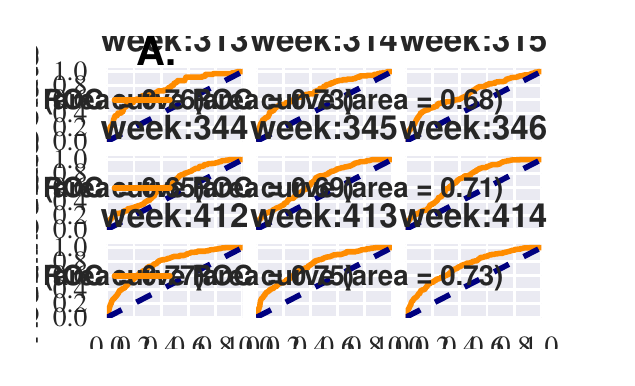
\begin{tikzpicture}[font=\bf\sffamily\fontsize{8}{8}\selectfont]
      \def\XST{-0.25in}
      \def\YST{0.25in}
      \node[] (A) {%% Creator: Matplotlib, PGF backend
%%
%% To include the figure in your LaTeX document, write
%%   \input{<filename>.pgf}
%%
%% Make sure the required packages are loaded in your preamble
%%   \usepackage{pgf}
%%
%% Figures using additional raster images can only be included by \input if
%% they are in the same directory as the main LaTeX file. For loading figures
%% from other directories you can use the `import` package
%%   \usepackage{import}
%% and then include the figures with
%%   \import{<path to file>}{<filename>.pgf}
%%
%% Matplotlib used the following preamble
%%   \usepackage[utf8x]{inputenc}
%%   \usepackage[T1]{fontenc}
%%
\begingroup%
\makeatletter%
\begin{pgfpicture}%
\pgfpathrectangle{\pgfpointorigin}{\pgfqpoint{2.801993in}{1.558554in}}%
\pgfusepath{use as bounding box, clip}%
\begin{pgfscope}%
\pgfsetbuttcap%
\pgfsetmiterjoin%
\definecolor{currentfill}{rgb}{1.000000,1.000000,1.000000}%
\pgfsetfillcolor{currentfill}%
\pgfsetlinewidth{0.000000pt}%
\definecolor{currentstroke}{rgb}{1.000000,1.000000,1.000000}%
\pgfsetstrokecolor{currentstroke}%
\pgfsetdash{}{0pt}%
\pgfpathmoveto{\pgfqpoint{0.000000in}{0.000000in}}%
\pgfpathlineto{\pgfqpoint{2.801993in}{0.000000in}}%
\pgfpathlineto{\pgfqpoint{2.801993in}{1.558554in}}%
\pgfpathlineto{\pgfqpoint{0.000000in}{1.558554in}}%
\pgfpathclose%
\pgfusepath{fill}%
\end{pgfscope}%
\begin{pgfscope}%
\pgfsetbuttcap%
\pgfsetmiterjoin%
\definecolor{currentfill}{rgb}{0.917647,0.917647,0.949020}%
\pgfsetfillcolor{currentfill}%
\pgfsetlinewidth{0.000000pt}%
\definecolor{currentstroke}{rgb}{0.000000,0.000000,0.000000}%
\pgfsetstrokecolor{currentstroke}%
\pgfsetstrokeopacity{0.000000}%
\pgfsetdash{}{0pt}%
\pgfpathmoveto{\pgfqpoint{0.350249in}{1.035980in}}%
\pgfpathlineto{\pgfqpoint{1.028857in}{1.035980in}}%
\pgfpathlineto{\pgfqpoint{1.028857in}{1.402699in}}%
\pgfpathlineto{\pgfqpoint{0.350249in}{1.402699in}}%
\pgfpathclose%
\pgfusepath{fill}%
\end{pgfscope}%
\begin{pgfscope}%
\pgfpathrectangle{\pgfqpoint{0.350249in}{1.035980in}}{\pgfqpoint{0.678608in}{0.366719in}} %
\pgfusepath{clip}%
\pgfsetroundcap%
\pgfsetroundjoin%
\pgfsetlinewidth{1.003750pt}%
\definecolor{currentstroke}{rgb}{1.000000,1.000000,1.000000}%
\pgfsetstrokecolor{currentstroke}%
\pgfsetdash{}{0pt}%
\pgfpathmoveto{\pgfqpoint{0.350249in}{1.035980in}}%
\pgfpathlineto{\pgfqpoint{0.350249in}{1.402699in}}%
\pgfusepath{stroke}%
\end{pgfscope}%
\begin{pgfscope}%
\pgfsetbuttcap%
\pgfsetroundjoin%
\definecolor{currentfill}{rgb}{0.150000,0.150000,0.150000}%
\pgfsetfillcolor{currentfill}%
\pgfsetlinewidth{1.003750pt}%
\definecolor{currentstroke}{rgb}{0.150000,0.150000,0.150000}%
\pgfsetstrokecolor{currentstroke}%
\pgfsetdash{}{0pt}%
\pgfsys@defobject{currentmarker}{\pgfqpoint{0.000000in}{0.000000in}}{\pgfqpoint{0.000000in}{0.000000in}}{%
\pgfpathmoveto{\pgfqpoint{0.000000in}{0.000000in}}%
\pgfpathlineto{\pgfqpoint{0.000000in}{0.000000in}}%
\pgfusepath{stroke,fill}%
}%
\begin{pgfscope}%
\pgfsys@transformshift{0.350249in}{1.035980in}%
\pgfsys@useobject{currentmarker}{}%
\end{pgfscope}%
\end{pgfscope}%
\begin{pgfscope}%
\pgfsetbuttcap%
\pgfsetroundjoin%
\definecolor{currentfill}{rgb}{0.150000,0.150000,0.150000}%
\pgfsetfillcolor{currentfill}%
\pgfsetlinewidth{1.003750pt}%
\definecolor{currentstroke}{rgb}{0.150000,0.150000,0.150000}%
\pgfsetstrokecolor{currentstroke}%
\pgfsetdash{}{0pt}%
\pgfsys@defobject{currentmarker}{\pgfqpoint{0.000000in}{0.000000in}}{\pgfqpoint{0.000000in}{0.000000in}}{%
\pgfpathmoveto{\pgfqpoint{0.000000in}{0.000000in}}%
\pgfpathlineto{\pgfqpoint{0.000000in}{0.000000in}}%
\pgfusepath{stroke,fill}%
}%
\begin{pgfscope}%
\pgfsys@transformshift{0.350249in}{1.402699in}%
\pgfsys@useobject{currentmarker}{}%
\end{pgfscope}%
\end{pgfscope}%
\begin{pgfscope}%
\pgfpathrectangle{\pgfqpoint{0.350249in}{1.035980in}}{\pgfqpoint{0.678608in}{0.366719in}} %
\pgfusepath{clip}%
\pgfsetroundcap%
\pgfsetroundjoin%
\pgfsetlinewidth{1.003750pt}%
\definecolor{currentstroke}{rgb}{1.000000,1.000000,1.000000}%
\pgfsetstrokecolor{currentstroke}%
\pgfsetdash{}{0pt}%
\pgfpathmoveto{\pgfqpoint{0.485971in}{1.035980in}}%
\pgfpathlineto{\pgfqpoint{0.485971in}{1.402699in}}%
\pgfusepath{stroke}%
\end{pgfscope}%
\begin{pgfscope}%
\pgfsetbuttcap%
\pgfsetroundjoin%
\definecolor{currentfill}{rgb}{0.150000,0.150000,0.150000}%
\pgfsetfillcolor{currentfill}%
\pgfsetlinewidth{1.003750pt}%
\definecolor{currentstroke}{rgb}{0.150000,0.150000,0.150000}%
\pgfsetstrokecolor{currentstroke}%
\pgfsetdash{}{0pt}%
\pgfsys@defobject{currentmarker}{\pgfqpoint{0.000000in}{0.000000in}}{\pgfqpoint{0.000000in}{0.000000in}}{%
\pgfpathmoveto{\pgfqpoint{0.000000in}{0.000000in}}%
\pgfpathlineto{\pgfqpoint{0.000000in}{0.000000in}}%
\pgfusepath{stroke,fill}%
}%
\begin{pgfscope}%
\pgfsys@transformshift{0.485971in}{1.035980in}%
\pgfsys@useobject{currentmarker}{}%
\end{pgfscope}%
\end{pgfscope}%
\begin{pgfscope}%
\pgfsetbuttcap%
\pgfsetroundjoin%
\definecolor{currentfill}{rgb}{0.150000,0.150000,0.150000}%
\pgfsetfillcolor{currentfill}%
\pgfsetlinewidth{1.003750pt}%
\definecolor{currentstroke}{rgb}{0.150000,0.150000,0.150000}%
\pgfsetstrokecolor{currentstroke}%
\pgfsetdash{}{0pt}%
\pgfsys@defobject{currentmarker}{\pgfqpoint{0.000000in}{0.000000in}}{\pgfqpoint{0.000000in}{0.000000in}}{%
\pgfpathmoveto{\pgfqpoint{0.000000in}{0.000000in}}%
\pgfpathlineto{\pgfqpoint{0.000000in}{0.000000in}}%
\pgfusepath{stroke,fill}%
}%
\begin{pgfscope}%
\pgfsys@transformshift{0.485971in}{1.402699in}%
\pgfsys@useobject{currentmarker}{}%
\end{pgfscope}%
\end{pgfscope}%
\begin{pgfscope}%
\pgfpathrectangle{\pgfqpoint{0.350249in}{1.035980in}}{\pgfqpoint{0.678608in}{0.366719in}} %
\pgfusepath{clip}%
\pgfsetroundcap%
\pgfsetroundjoin%
\pgfsetlinewidth{1.003750pt}%
\definecolor{currentstroke}{rgb}{1.000000,1.000000,1.000000}%
\pgfsetstrokecolor{currentstroke}%
\pgfsetdash{}{0pt}%
\pgfpathmoveto{\pgfqpoint{0.621692in}{1.035980in}}%
\pgfpathlineto{\pgfqpoint{0.621692in}{1.402699in}}%
\pgfusepath{stroke}%
\end{pgfscope}%
\begin{pgfscope}%
\pgfsetbuttcap%
\pgfsetroundjoin%
\definecolor{currentfill}{rgb}{0.150000,0.150000,0.150000}%
\pgfsetfillcolor{currentfill}%
\pgfsetlinewidth{1.003750pt}%
\definecolor{currentstroke}{rgb}{0.150000,0.150000,0.150000}%
\pgfsetstrokecolor{currentstroke}%
\pgfsetdash{}{0pt}%
\pgfsys@defobject{currentmarker}{\pgfqpoint{0.000000in}{0.000000in}}{\pgfqpoint{0.000000in}{0.000000in}}{%
\pgfpathmoveto{\pgfqpoint{0.000000in}{0.000000in}}%
\pgfpathlineto{\pgfqpoint{0.000000in}{0.000000in}}%
\pgfusepath{stroke,fill}%
}%
\begin{pgfscope}%
\pgfsys@transformshift{0.621692in}{1.035980in}%
\pgfsys@useobject{currentmarker}{}%
\end{pgfscope}%
\end{pgfscope}%
\begin{pgfscope}%
\pgfsetbuttcap%
\pgfsetroundjoin%
\definecolor{currentfill}{rgb}{0.150000,0.150000,0.150000}%
\pgfsetfillcolor{currentfill}%
\pgfsetlinewidth{1.003750pt}%
\definecolor{currentstroke}{rgb}{0.150000,0.150000,0.150000}%
\pgfsetstrokecolor{currentstroke}%
\pgfsetdash{}{0pt}%
\pgfsys@defobject{currentmarker}{\pgfqpoint{0.000000in}{0.000000in}}{\pgfqpoint{0.000000in}{0.000000in}}{%
\pgfpathmoveto{\pgfqpoint{0.000000in}{0.000000in}}%
\pgfpathlineto{\pgfqpoint{0.000000in}{0.000000in}}%
\pgfusepath{stroke,fill}%
}%
\begin{pgfscope}%
\pgfsys@transformshift{0.621692in}{1.402699in}%
\pgfsys@useobject{currentmarker}{}%
\end{pgfscope}%
\end{pgfscope}%
\begin{pgfscope}%
\pgfpathrectangle{\pgfqpoint{0.350249in}{1.035980in}}{\pgfqpoint{0.678608in}{0.366719in}} %
\pgfusepath{clip}%
\pgfsetroundcap%
\pgfsetroundjoin%
\pgfsetlinewidth{1.003750pt}%
\definecolor{currentstroke}{rgb}{1.000000,1.000000,1.000000}%
\pgfsetstrokecolor{currentstroke}%
\pgfsetdash{}{0pt}%
\pgfpathmoveto{\pgfqpoint{0.757414in}{1.035980in}}%
\pgfpathlineto{\pgfqpoint{0.757414in}{1.402699in}}%
\pgfusepath{stroke}%
\end{pgfscope}%
\begin{pgfscope}%
\pgfsetbuttcap%
\pgfsetroundjoin%
\definecolor{currentfill}{rgb}{0.150000,0.150000,0.150000}%
\pgfsetfillcolor{currentfill}%
\pgfsetlinewidth{1.003750pt}%
\definecolor{currentstroke}{rgb}{0.150000,0.150000,0.150000}%
\pgfsetstrokecolor{currentstroke}%
\pgfsetdash{}{0pt}%
\pgfsys@defobject{currentmarker}{\pgfqpoint{0.000000in}{0.000000in}}{\pgfqpoint{0.000000in}{0.000000in}}{%
\pgfpathmoveto{\pgfqpoint{0.000000in}{0.000000in}}%
\pgfpathlineto{\pgfqpoint{0.000000in}{0.000000in}}%
\pgfusepath{stroke,fill}%
}%
\begin{pgfscope}%
\pgfsys@transformshift{0.757414in}{1.035980in}%
\pgfsys@useobject{currentmarker}{}%
\end{pgfscope}%
\end{pgfscope}%
\begin{pgfscope}%
\pgfsetbuttcap%
\pgfsetroundjoin%
\definecolor{currentfill}{rgb}{0.150000,0.150000,0.150000}%
\pgfsetfillcolor{currentfill}%
\pgfsetlinewidth{1.003750pt}%
\definecolor{currentstroke}{rgb}{0.150000,0.150000,0.150000}%
\pgfsetstrokecolor{currentstroke}%
\pgfsetdash{}{0pt}%
\pgfsys@defobject{currentmarker}{\pgfqpoint{0.000000in}{0.000000in}}{\pgfqpoint{0.000000in}{0.000000in}}{%
\pgfpathmoveto{\pgfqpoint{0.000000in}{0.000000in}}%
\pgfpathlineto{\pgfqpoint{0.000000in}{0.000000in}}%
\pgfusepath{stroke,fill}%
}%
\begin{pgfscope}%
\pgfsys@transformshift{0.757414in}{1.402699in}%
\pgfsys@useobject{currentmarker}{}%
\end{pgfscope}%
\end{pgfscope}%
\begin{pgfscope}%
\pgfpathrectangle{\pgfqpoint{0.350249in}{1.035980in}}{\pgfqpoint{0.678608in}{0.366719in}} %
\pgfusepath{clip}%
\pgfsetroundcap%
\pgfsetroundjoin%
\pgfsetlinewidth{1.003750pt}%
\definecolor{currentstroke}{rgb}{1.000000,1.000000,1.000000}%
\pgfsetstrokecolor{currentstroke}%
\pgfsetdash{}{0pt}%
\pgfpathmoveto{\pgfqpoint{0.893135in}{1.035980in}}%
\pgfpathlineto{\pgfqpoint{0.893135in}{1.402699in}}%
\pgfusepath{stroke}%
\end{pgfscope}%
\begin{pgfscope}%
\pgfsetbuttcap%
\pgfsetroundjoin%
\definecolor{currentfill}{rgb}{0.150000,0.150000,0.150000}%
\pgfsetfillcolor{currentfill}%
\pgfsetlinewidth{1.003750pt}%
\definecolor{currentstroke}{rgb}{0.150000,0.150000,0.150000}%
\pgfsetstrokecolor{currentstroke}%
\pgfsetdash{}{0pt}%
\pgfsys@defobject{currentmarker}{\pgfqpoint{0.000000in}{0.000000in}}{\pgfqpoint{0.000000in}{0.000000in}}{%
\pgfpathmoveto{\pgfqpoint{0.000000in}{0.000000in}}%
\pgfpathlineto{\pgfqpoint{0.000000in}{0.000000in}}%
\pgfusepath{stroke,fill}%
}%
\begin{pgfscope}%
\pgfsys@transformshift{0.893135in}{1.035980in}%
\pgfsys@useobject{currentmarker}{}%
\end{pgfscope}%
\end{pgfscope}%
\begin{pgfscope}%
\pgfsetbuttcap%
\pgfsetroundjoin%
\definecolor{currentfill}{rgb}{0.150000,0.150000,0.150000}%
\pgfsetfillcolor{currentfill}%
\pgfsetlinewidth{1.003750pt}%
\definecolor{currentstroke}{rgb}{0.150000,0.150000,0.150000}%
\pgfsetstrokecolor{currentstroke}%
\pgfsetdash{}{0pt}%
\pgfsys@defobject{currentmarker}{\pgfqpoint{0.000000in}{0.000000in}}{\pgfqpoint{0.000000in}{0.000000in}}{%
\pgfpathmoveto{\pgfqpoint{0.000000in}{0.000000in}}%
\pgfpathlineto{\pgfqpoint{0.000000in}{0.000000in}}%
\pgfusepath{stroke,fill}%
}%
\begin{pgfscope}%
\pgfsys@transformshift{0.893135in}{1.402699in}%
\pgfsys@useobject{currentmarker}{}%
\end{pgfscope}%
\end{pgfscope}%
\begin{pgfscope}%
\pgfpathrectangle{\pgfqpoint{0.350249in}{1.035980in}}{\pgfqpoint{0.678608in}{0.366719in}} %
\pgfusepath{clip}%
\pgfsetroundcap%
\pgfsetroundjoin%
\pgfsetlinewidth{1.003750pt}%
\definecolor{currentstroke}{rgb}{1.000000,1.000000,1.000000}%
\pgfsetstrokecolor{currentstroke}%
\pgfsetdash{}{0pt}%
\pgfpathmoveto{\pgfqpoint{1.028857in}{1.035980in}}%
\pgfpathlineto{\pgfqpoint{1.028857in}{1.402699in}}%
\pgfusepath{stroke}%
\end{pgfscope}%
\begin{pgfscope}%
\pgfsetbuttcap%
\pgfsetroundjoin%
\definecolor{currentfill}{rgb}{0.150000,0.150000,0.150000}%
\pgfsetfillcolor{currentfill}%
\pgfsetlinewidth{1.003750pt}%
\definecolor{currentstroke}{rgb}{0.150000,0.150000,0.150000}%
\pgfsetstrokecolor{currentstroke}%
\pgfsetdash{}{0pt}%
\pgfsys@defobject{currentmarker}{\pgfqpoint{0.000000in}{0.000000in}}{\pgfqpoint{0.000000in}{0.000000in}}{%
\pgfpathmoveto{\pgfqpoint{0.000000in}{0.000000in}}%
\pgfpathlineto{\pgfqpoint{0.000000in}{0.000000in}}%
\pgfusepath{stroke,fill}%
}%
\begin{pgfscope}%
\pgfsys@transformshift{1.028857in}{1.035980in}%
\pgfsys@useobject{currentmarker}{}%
\end{pgfscope}%
\end{pgfscope}%
\begin{pgfscope}%
\pgfsetbuttcap%
\pgfsetroundjoin%
\definecolor{currentfill}{rgb}{0.150000,0.150000,0.150000}%
\pgfsetfillcolor{currentfill}%
\pgfsetlinewidth{1.003750pt}%
\definecolor{currentstroke}{rgb}{0.150000,0.150000,0.150000}%
\pgfsetstrokecolor{currentstroke}%
\pgfsetdash{}{0pt}%
\pgfsys@defobject{currentmarker}{\pgfqpoint{0.000000in}{0.000000in}}{\pgfqpoint{0.000000in}{0.000000in}}{%
\pgfpathmoveto{\pgfqpoint{0.000000in}{0.000000in}}%
\pgfpathlineto{\pgfqpoint{0.000000in}{0.000000in}}%
\pgfusepath{stroke,fill}%
}%
\begin{pgfscope}%
\pgfsys@transformshift{1.028857in}{1.402699in}%
\pgfsys@useobject{currentmarker}{}%
\end{pgfscope}%
\end{pgfscope}%
\begin{pgfscope}%
\pgfpathrectangle{\pgfqpoint{0.350249in}{1.035980in}}{\pgfqpoint{0.678608in}{0.366719in}} %
\pgfusepath{clip}%
\pgfsetroundcap%
\pgfsetroundjoin%
\pgfsetlinewidth{1.003750pt}%
\definecolor{currentstroke}{rgb}{1.000000,1.000000,1.000000}%
\pgfsetstrokecolor{currentstroke}%
\pgfsetdash{}{0pt}%
\pgfpathmoveto{\pgfqpoint{0.350249in}{1.035980in}}%
\pgfpathlineto{\pgfqpoint{1.028857in}{1.035980in}}%
\pgfusepath{stroke}%
\end{pgfscope}%
\begin{pgfscope}%
\pgfsetbuttcap%
\pgfsetroundjoin%
\definecolor{currentfill}{rgb}{0.150000,0.150000,0.150000}%
\pgfsetfillcolor{currentfill}%
\pgfsetlinewidth{1.003750pt}%
\definecolor{currentstroke}{rgb}{0.150000,0.150000,0.150000}%
\pgfsetstrokecolor{currentstroke}%
\pgfsetdash{}{0pt}%
\pgfsys@defobject{currentmarker}{\pgfqpoint{0.000000in}{0.000000in}}{\pgfqpoint{0.000000in}{0.000000in}}{%
\pgfpathmoveto{\pgfqpoint{0.000000in}{0.000000in}}%
\pgfpathlineto{\pgfqpoint{0.000000in}{0.000000in}}%
\pgfusepath{stroke,fill}%
}%
\begin{pgfscope}%
\pgfsys@transformshift{0.350249in}{1.035980in}%
\pgfsys@useobject{currentmarker}{}%
\end{pgfscope}%
\end{pgfscope}%
\begin{pgfscope}%
\pgfsetbuttcap%
\pgfsetroundjoin%
\definecolor{currentfill}{rgb}{0.150000,0.150000,0.150000}%
\pgfsetfillcolor{currentfill}%
\pgfsetlinewidth{1.003750pt}%
\definecolor{currentstroke}{rgb}{0.150000,0.150000,0.150000}%
\pgfsetstrokecolor{currentstroke}%
\pgfsetdash{}{0pt}%
\pgfsys@defobject{currentmarker}{\pgfqpoint{0.000000in}{0.000000in}}{\pgfqpoint{0.000000in}{0.000000in}}{%
\pgfpathmoveto{\pgfqpoint{0.000000in}{0.000000in}}%
\pgfpathlineto{\pgfqpoint{0.000000in}{0.000000in}}%
\pgfusepath{stroke,fill}%
}%
\begin{pgfscope}%
\pgfsys@transformshift{1.028857in}{1.035980in}%
\pgfsys@useobject{currentmarker}{}%
\end{pgfscope}%
\end{pgfscope}%
\begin{pgfscope}%
\definecolor{textcolor}{rgb}{0.150000,0.150000,0.150000}%
\pgfsetstrokecolor{textcolor}%
\pgfsetfillcolor{textcolor}%
\pgftext[x=0.253027in,y=1.035980in,right,]{\color{textcolor}\sffamily\fontsize{10.000000}{12.000000}\bfseries\selectfont \(\displaystyle 0.0\)}%
\end{pgfscope}%
\begin{pgfscope}%
\pgfpathrectangle{\pgfqpoint{0.350249in}{1.035980in}}{\pgfqpoint{0.678608in}{0.366719in}} %
\pgfusepath{clip}%
\pgfsetroundcap%
\pgfsetroundjoin%
\pgfsetlinewidth{1.003750pt}%
\definecolor{currentstroke}{rgb}{1.000000,1.000000,1.000000}%
\pgfsetstrokecolor{currentstroke}%
\pgfsetdash{}{0pt}%
\pgfpathmoveto{\pgfqpoint{0.350249in}{1.105831in}}%
\pgfpathlineto{\pgfqpoint{1.028857in}{1.105831in}}%
\pgfusepath{stroke}%
\end{pgfscope}%
\begin{pgfscope}%
\pgfsetbuttcap%
\pgfsetroundjoin%
\definecolor{currentfill}{rgb}{0.150000,0.150000,0.150000}%
\pgfsetfillcolor{currentfill}%
\pgfsetlinewidth{1.003750pt}%
\definecolor{currentstroke}{rgb}{0.150000,0.150000,0.150000}%
\pgfsetstrokecolor{currentstroke}%
\pgfsetdash{}{0pt}%
\pgfsys@defobject{currentmarker}{\pgfqpoint{0.000000in}{0.000000in}}{\pgfqpoint{0.000000in}{0.000000in}}{%
\pgfpathmoveto{\pgfqpoint{0.000000in}{0.000000in}}%
\pgfpathlineto{\pgfqpoint{0.000000in}{0.000000in}}%
\pgfusepath{stroke,fill}%
}%
\begin{pgfscope}%
\pgfsys@transformshift{0.350249in}{1.105831in}%
\pgfsys@useobject{currentmarker}{}%
\end{pgfscope}%
\end{pgfscope}%
\begin{pgfscope}%
\pgfsetbuttcap%
\pgfsetroundjoin%
\definecolor{currentfill}{rgb}{0.150000,0.150000,0.150000}%
\pgfsetfillcolor{currentfill}%
\pgfsetlinewidth{1.003750pt}%
\definecolor{currentstroke}{rgb}{0.150000,0.150000,0.150000}%
\pgfsetstrokecolor{currentstroke}%
\pgfsetdash{}{0pt}%
\pgfsys@defobject{currentmarker}{\pgfqpoint{0.000000in}{0.000000in}}{\pgfqpoint{0.000000in}{0.000000in}}{%
\pgfpathmoveto{\pgfqpoint{0.000000in}{0.000000in}}%
\pgfpathlineto{\pgfqpoint{0.000000in}{0.000000in}}%
\pgfusepath{stroke,fill}%
}%
\begin{pgfscope}%
\pgfsys@transformshift{1.028857in}{1.105831in}%
\pgfsys@useobject{currentmarker}{}%
\end{pgfscope}%
\end{pgfscope}%
\begin{pgfscope}%
\definecolor{textcolor}{rgb}{0.150000,0.150000,0.150000}%
\pgfsetstrokecolor{textcolor}%
\pgfsetfillcolor{textcolor}%
\pgftext[x=0.253027in,y=1.105831in,right,]{\color{textcolor}\sffamily\fontsize{10.000000}{12.000000}\bfseries\selectfont \(\displaystyle 0.2\)}%
\end{pgfscope}%
\begin{pgfscope}%
\pgfpathrectangle{\pgfqpoint{0.350249in}{1.035980in}}{\pgfqpoint{0.678608in}{0.366719in}} %
\pgfusepath{clip}%
\pgfsetroundcap%
\pgfsetroundjoin%
\pgfsetlinewidth{1.003750pt}%
\definecolor{currentstroke}{rgb}{1.000000,1.000000,1.000000}%
\pgfsetstrokecolor{currentstroke}%
\pgfsetdash{}{0pt}%
\pgfpathmoveto{\pgfqpoint{0.350249in}{1.175682in}}%
\pgfpathlineto{\pgfqpoint{1.028857in}{1.175682in}}%
\pgfusepath{stroke}%
\end{pgfscope}%
\begin{pgfscope}%
\pgfsetbuttcap%
\pgfsetroundjoin%
\definecolor{currentfill}{rgb}{0.150000,0.150000,0.150000}%
\pgfsetfillcolor{currentfill}%
\pgfsetlinewidth{1.003750pt}%
\definecolor{currentstroke}{rgb}{0.150000,0.150000,0.150000}%
\pgfsetstrokecolor{currentstroke}%
\pgfsetdash{}{0pt}%
\pgfsys@defobject{currentmarker}{\pgfqpoint{0.000000in}{0.000000in}}{\pgfqpoint{0.000000in}{0.000000in}}{%
\pgfpathmoveto{\pgfqpoint{0.000000in}{0.000000in}}%
\pgfpathlineto{\pgfqpoint{0.000000in}{0.000000in}}%
\pgfusepath{stroke,fill}%
}%
\begin{pgfscope}%
\pgfsys@transformshift{0.350249in}{1.175682in}%
\pgfsys@useobject{currentmarker}{}%
\end{pgfscope}%
\end{pgfscope}%
\begin{pgfscope}%
\pgfsetbuttcap%
\pgfsetroundjoin%
\definecolor{currentfill}{rgb}{0.150000,0.150000,0.150000}%
\pgfsetfillcolor{currentfill}%
\pgfsetlinewidth{1.003750pt}%
\definecolor{currentstroke}{rgb}{0.150000,0.150000,0.150000}%
\pgfsetstrokecolor{currentstroke}%
\pgfsetdash{}{0pt}%
\pgfsys@defobject{currentmarker}{\pgfqpoint{0.000000in}{0.000000in}}{\pgfqpoint{0.000000in}{0.000000in}}{%
\pgfpathmoveto{\pgfqpoint{0.000000in}{0.000000in}}%
\pgfpathlineto{\pgfqpoint{0.000000in}{0.000000in}}%
\pgfusepath{stroke,fill}%
}%
\begin{pgfscope}%
\pgfsys@transformshift{1.028857in}{1.175682in}%
\pgfsys@useobject{currentmarker}{}%
\end{pgfscope}%
\end{pgfscope}%
\begin{pgfscope}%
\definecolor{textcolor}{rgb}{0.150000,0.150000,0.150000}%
\pgfsetstrokecolor{textcolor}%
\pgfsetfillcolor{textcolor}%
\pgftext[x=0.253027in,y=1.175682in,right,]{\color{textcolor}\sffamily\fontsize{10.000000}{12.000000}\bfseries\selectfont \(\displaystyle 0.4\)}%
\end{pgfscope}%
\begin{pgfscope}%
\pgfpathrectangle{\pgfqpoint{0.350249in}{1.035980in}}{\pgfqpoint{0.678608in}{0.366719in}} %
\pgfusepath{clip}%
\pgfsetroundcap%
\pgfsetroundjoin%
\pgfsetlinewidth{1.003750pt}%
\definecolor{currentstroke}{rgb}{1.000000,1.000000,1.000000}%
\pgfsetstrokecolor{currentstroke}%
\pgfsetdash{}{0pt}%
\pgfpathmoveto{\pgfqpoint{0.350249in}{1.245533in}}%
\pgfpathlineto{\pgfqpoint{1.028857in}{1.245533in}}%
\pgfusepath{stroke}%
\end{pgfscope}%
\begin{pgfscope}%
\pgfsetbuttcap%
\pgfsetroundjoin%
\definecolor{currentfill}{rgb}{0.150000,0.150000,0.150000}%
\pgfsetfillcolor{currentfill}%
\pgfsetlinewidth{1.003750pt}%
\definecolor{currentstroke}{rgb}{0.150000,0.150000,0.150000}%
\pgfsetstrokecolor{currentstroke}%
\pgfsetdash{}{0pt}%
\pgfsys@defobject{currentmarker}{\pgfqpoint{0.000000in}{0.000000in}}{\pgfqpoint{0.000000in}{0.000000in}}{%
\pgfpathmoveto{\pgfqpoint{0.000000in}{0.000000in}}%
\pgfpathlineto{\pgfqpoint{0.000000in}{0.000000in}}%
\pgfusepath{stroke,fill}%
}%
\begin{pgfscope}%
\pgfsys@transformshift{0.350249in}{1.245533in}%
\pgfsys@useobject{currentmarker}{}%
\end{pgfscope}%
\end{pgfscope}%
\begin{pgfscope}%
\pgfsetbuttcap%
\pgfsetroundjoin%
\definecolor{currentfill}{rgb}{0.150000,0.150000,0.150000}%
\pgfsetfillcolor{currentfill}%
\pgfsetlinewidth{1.003750pt}%
\definecolor{currentstroke}{rgb}{0.150000,0.150000,0.150000}%
\pgfsetstrokecolor{currentstroke}%
\pgfsetdash{}{0pt}%
\pgfsys@defobject{currentmarker}{\pgfqpoint{0.000000in}{0.000000in}}{\pgfqpoint{0.000000in}{0.000000in}}{%
\pgfpathmoveto{\pgfqpoint{0.000000in}{0.000000in}}%
\pgfpathlineto{\pgfqpoint{0.000000in}{0.000000in}}%
\pgfusepath{stroke,fill}%
}%
\begin{pgfscope}%
\pgfsys@transformshift{1.028857in}{1.245533in}%
\pgfsys@useobject{currentmarker}{}%
\end{pgfscope}%
\end{pgfscope}%
\begin{pgfscope}%
\definecolor{textcolor}{rgb}{0.150000,0.150000,0.150000}%
\pgfsetstrokecolor{textcolor}%
\pgfsetfillcolor{textcolor}%
\pgftext[x=0.253027in,y=1.245533in,right,]{\color{textcolor}\sffamily\fontsize{10.000000}{12.000000}\bfseries\selectfont \(\displaystyle 0.6\)}%
\end{pgfscope}%
\begin{pgfscope}%
\pgfpathrectangle{\pgfqpoint{0.350249in}{1.035980in}}{\pgfqpoint{0.678608in}{0.366719in}} %
\pgfusepath{clip}%
\pgfsetroundcap%
\pgfsetroundjoin%
\pgfsetlinewidth{1.003750pt}%
\definecolor{currentstroke}{rgb}{1.000000,1.000000,1.000000}%
\pgfsetstrokecolor{currentstroke}%
\pgfsetdash{}{0pt}%
\pgfpathmoveto{\pgfqpoint{0.350249in}{1.315385in}}%
\pgfpathlineto{\pgfqpoint{1.028857in}{1.315385in}}%
\pgfusepath{stroke}%
\end{pgfscope}%
\begin{pgfscope}%
\pgfsetbuttcap%
\pgfsetroundjoin%
\definecolor{currentfill}{rgb}{0.150000,0.150000,0.150000}%
\pgfsetfillcolor{currentfill}%
\pgfsetlinewidth{1.003750pt}%
\definecolor{currentstroke}{rgb}{0.150000,0.150000,0.150000}%
\pgfsetstrokecolor{currentstroke}%
\pgfsetdash{}{0pt}%
\pgfsys@defobject{currentmarker}{\pgfqpoint{0.000000in}{0.000000in}}{\pgfqpoint{0.000000in}{0.000000in}}{%
\pgfpathmoveto{\pgfqpoint{0.000000in}{0.000000in}}%
\pgfpathlineto{\pgfqpoint{0.000000in}{0.000000in}}%
\pgfusepath{stroke,fill}%
}%
\begin{pgfscope}%
\pgfsys@transformshift{0.350249in}{1.315385in}%
\pgfsys@useobject{currentmarker}{}%
\end{pgfscope}%
\end{pgfscope}%
\begin{pgfscope}%
\pgfsetbuttcap%
\pgfsetroundjoin%
\definecolor{currentfill}{rgb}{0.150000,0.150000,0.150000}%
\pgfsetfillcolor{currentfill}%
\pgfsetlinewidth{1.003750pt}%
\definecolor{currentstroke}{rgb}{0.150000,0.150000,0.150000}%
\pgfsetstrokecolor{currentstroke}%
\pgfsetdash{}{0pt}%
\pgfsys@defobject{currentmarker}{\pgfqpoint{0.000000in}{0.000000in}}{\pgfqpoint{0.000000in}{0.000000in}}{%
\pgfpathmoveto{\pgfqpoint{0.000000in}{0.000000in}}%
\pgfpathlineto{\pgfqpoint{0.000000in}{0.000000in}}%
\pgfusepath{stroke,fill}%
}%
\begin{pgfscope}%
\pgfsys@transformshift{1.028857in}{1.315385in}%
\pgfsys@useobject{currentmarker}{}%
\end{pgfscope}%
\end{pgfscope}%
\begin{pgfscope}%
\definecolor{textcolor}{rgb}{0.150000,0.150000,0.150000}%
\pgfsetstrokecolor{textcolor}%
\pgfsetfillcolor{textcolor}%
\pgftext[x=0.253027in,y=1.315385in,right,]{\color{textcolor}\sffamily\fontsize{10.000000}{12.000000}\bfseries\selectfont \(\displaystyle 0.8\)}%
\end{pgfscope}%
\begin{pgfscope}%
\pgfpathrectangle{\pgfqpoint{0.350249in}{1.035980in}}{\pgfqpoint{0.678608in}{0.366719in}} %
\pgfusepath{clip}%
\pgfsetroundcap%
\pgfsetroundjoin%
\pgfsetlinewidth{1.003750pt}%
\definecolor{currentstroke}{rgb}{1.000000,1.000000,1.000000}%
\pgfsetstrokecolor{currentstroke}%
\pgfsetdash{}{0pt}%
\pgfpathmoveto{\pgfqpoint{0.350249in}{1.385236in}}%
\pgfpathlineto{\pgfqpoint{1.028857in}{1.385236in}}%
\pgfusepath{stroke}%
\end{pgfscope}%
\begin{pgfscope}%
\pgfsetbuttcap%
\pgfsetroundjoin%
\definecolor{currentfill}{rgb}{0.150000,0.150000,0.150000}%
\pgfsetfillcolor{currentfill}%
\pgfsetlinewidth{1.003750pt}%
\definecolor{currentstroke}{rgb}{0.150000,0.150000,0.150000}%
\pgfsetstrokecolor{currentstroke}%
\pgfsetdash{}{0pt}%
\pgfsys@defobject{currentmarker}{\pgfqpoint{0.000000in}{0.000000in}}{\pgfqpoint{0.000000in}{0.000000in}}{%
\pgfpathmoveto{\pgfqpoint{0.000000in}{0.000000in}}%
\pgfpathlineto{\pgfqpoint{0.000000in}{0.000000in}}%
\pgfusepath{stroke,fill}%
}%
\begin{pgfscope}%
\pgfsys@transformshift{0.350249in}{1.385236in}%
\pgfsys@useobject{currentmarker}{}%
\end{pgfscope}%
\end{pgfscope}%
\begin{pgfscope}%
\pgfsetbuttcap%
\pgfsetroundjoin%
\definecolor{currentfill}{rgb}{0.150000,0.150000,0.150000}%
\pgfsetfillcolor{currentfill}%
\pgfsetlinewidth{1.003750pt}%
\definecolor{currentstroke}{rgb}{0.150000,0.150000,0.150000}%
\pgfsetstrokecolor{currentstroke}%
\pgfsetdash{}{0pt}%
\pgfsys@defobject{currentmarker}{\pgfqpoint{0.000000in}{0.000000in}}{\pgfqpoint{0.000000in}{0.000000in}}{%
\pgfpathmoveto{\pgfqpoint{0.000000in}{0.000000in}}%
\pgfpathlineto{\pgfqpoint{0.000000in}{0.000000in}}%
\pgfusepath{stroke,fill}%
}%
\begin{pgfscope}%
\pgfsys@transformshift{1.028857in}{1.385236in}%
\pgfsys@useobject{currentmarker}{}%
\end{pgfscope}%
\end{pgfscope}%
\begin{pgfscope}%
\definecolor{textcolor}{rgb}{0.150000,0.150000,0.150000}%
\pgfsetstrokecolor{textcolor}%
\pgfsetfillcolor{textcolor}%
\pgftext[x=0.253027in,y=1.385236in,right,]{\color{textcolor}\sffamily\fontsize{10.000000}{12.000000}\bfseries\selectfont \(\displaystyle 1.0\)}%
\end{pgfscope}%
\begin{pgfscope}%
\definecolor{textcolor}{rgb}{0.150000,0.150000,0.150000}%
\pgfsetstrokecolor{textcolor}%
\pgfsetfillcolor{textcolor}%
\pgftext[x=0.006113in,y=1.219339in,,bottom,rotate=90.000000]{\color{textcolor}\sffamily\fontsize{12.000000}{14.400000}\bfseries\selectfont True Positive Rate}%
\end{pgfscope}%
\begin{pgfscope}%
\pgfpathrectangle{\pgfqpoint{0.350249in}{1.035980in}}{\pgfqpoint{0.678608in}{0.366719in}} %
\pgfusepath{clip}%
\pgfsetroundcap%
\pgfsetroundjoin%
\pgfsetlinewidth{2.007500pt}%
\definecolor{currentstroke}{rgb}{1.000000,0.549020,0.000000}%
\pgfsetstrokecolor{currentstroke}%
\pgfsetdash{}{0pt}%
\pgfpathmoveto{\pgfqpoint{0.350249in}{1.039438in}}%
\pgfpathlineto{\pgfqpoint{0.350479in}{1.039438in}}%
\pgfpathlineto{\pgfqpoint{0.350709in}{1.049812in}}%
\pgfpathlineto{\pgfqpoint{0.351860in}{1.049812in}}%
\pgfpathlineto{\pgfqpoint{0.352780in}{1.060186in}}%
\pgfpathlineto{\pgfqpoint{0.353471in}{1.060186in}}%
\pgfpathlineto{\pgfqpoint{0.353471in}{1.063644in}}%
\pgfpathlineto{\pgfqpoint{0.355312in}{1.063644in}}%
\pgfpathlineto{\pgfqpoint{0.355312in}{1.067102in}}%
\pgfpathlineto{\pgfqpoint{0.356692in}{1.067102in}}%
\pgfpathlineto{\pgfqpoint{0.356692in}{1.070560in}}%
\pgfpathlineto{\pgfqpoint{0.357843in}{1.070560in}}%
\pgfpathlineto{\pgfqpoint{0.357843in}{1.074018in}}%
\pgfpathlineto{\pgfqpoint{0.360144in}{1.074018in}}%
\pgfpathlineto{\pgfqpoint{0.360834in}{1.091308in}}%
\pgfpathlineto{\pgfqpoint{0.361525in}{1.091308in}}%
\pgfpathlineto{\pgfqpoint{0.361525in}{1.094766in}}%
\pgfpathlineto{\pgfqpoint{0.363826in}{1.094766in}}%
\pgfpathlineto{\pgfqpoint{0.364056in}{1.101682in}}%
\pgfpathlineto{\pgfqpoint{0.366587in}{1.101682in}}%
\pgfpathlineto{\pgfqpoint{0.366817in}{1.108598in}}%
\pgfpathlineto{\pgfqpoint{0.369579in}{1.108598in}}%
\pgfpathlineto{\pgfqpoint{0.369579in}{1.112056in}}%
\pgfpathlineto{\pgfqpoint{0.372570in}{1.112056in}}%
\pgfpathlineto{\pgfqpoint{0.372570in}{1.115513in}}%
\pgfpathlineto{\pgfqpoint{0.376022in}{1.115513in}}%
\pgfpathlineto{\pgfqpoint{0.376942in}{1.122429in}}%
\pgfpathlineto{\pgfqpoint{0.377403in}{1.122429in}}%
\pgfpathlineto{\pgfqpoint{0.377403in}{1.125887in}}%
\pgfpathlineto{\pgfqpoint{0.379704in}{1.125887in}}%
\pgfpathlineto{\pgfqpoint{0.379704in}{1.129345in}}%
\pgfpathlineto{\pgfqpoint{0.381545in}{1.129345in}}%
\pgfpathlineto{\pgfqpoint{0.382235in}{1.139719in}}%
\pgfpathlineto{\pgfqpoint{0.382695in}{1.139719in}}%
\pgfpathlineto{\pgfqpoint{0.383616in}{1.146635in}}%
\pgfpathlineto{\pgfqpoint{0.384536in}{1.146635in}}%
\pgfpathlineto{\pgfqpoint{0.384536in}{1.150093in}}%
\pgfpathlineto{\pgfqpoint{0.385917in}{1.150093in}}%
\pgfpathlineto{\pgfqpoint{0.385917in}{1.153551in}}%
\pgfpathlineto{\pgfqpoint{0.387988in}{1.153551in}}%
\pgfpathlineto{\pgfqpoint{0.387988in}{1.157009in}}%
\pgfpathlineto{\pgfqpoint{0.389138in}{1.157009in}}%
\pgfpathlineto{\pgfqpoint{0.389138in}{1.160467in}}%
\pgfpathlineto{\pgfqpoint{0.390059in}{1.160467in}}%
\pgfpathlineto{\pgfqpoint{0.390289in}{1.160467in}}%
\pgfpathlineto{\pgfqpoint{0.390289in}{1.163925in}}%
\pgfpathlineto{\pgfqpoint{0.400184in}{1.163925in}}%
\pgfpathlineto{\pgfqpoint{0.400184in}{1.167383in}}%
\pgfpathlineto{\pgfqpoint{0.402945in}{1.167383in}}%
\pgfpathlineto{\pgfqpoint{0.402945in}{1.170841in}}%
\pgfpathlineto{\pgfqpoint{0.404556in}{1.170841in}}%
\pgfpathlineto{\pgfqpoint{0.405246in}{1.177757in}}%
\pgfpathlineto{\pgfqpoint{0.421815in}{1.177757in}}%
\pgfpathlineto{\pgfqpoint{0.422045in}{1.184673in}}%
\pgfpathlineto{\pgfqpoint{0.429408in}{1.184673in}}%
\pgfpathlineto{\pgfqpoint{0.429869in}{1.188131in}}%
\pgfpathlineto{\pgfqpoint{0.431249in}{1.188131in}}%
\pgfpathlineto{\pgfqpoint{0.432170in}{1.198505in}}%
\pgfpathlineto{\pgfqpoint{0.432400in}{1.198505in}}%
\pgfpathlineto{\pgfqpoint{0.432400in}{1.201963in}}%
\pgfpathlineto{\pgfqpoint{0.434701in}{1.201963in}}%
\pgfpathlineto{\pgfqpoint{0.434701in}{1.205421in}}%
\pgfpathlineto{\pgfqpoint{0.439764in}{1.205421in}}%
\pgfpathlineto{\pgfqpoint{0.439764in}{1.208879in}}%
\pgfpathlineto{\pgfqpoint{0.445977in}{1.208879in}}%
\pgfpathlineto{\pgfqpoint{0.445977in}{1.215795in}}%
\pgfpathlineto{\pgfqpoint{0.449659in}{1.215795in}}%
\pgfpathlineto{\pgfqpoint{0.449659in}{1.219253in}}%
\pgfpathlineto{\pgfqpoint{0.452650in}{1.219253in}}%
\pgfpathlineto{\pgfqpoint{0.452650in}{1.222711in}}%
\pgfpathlineto{\pgfqpoint{0.462315in}{1.222711in}}%
\pgfpathlineto{\pgfqpoint{0.462315in}{1.226169in}}%
\pgfpathlineto{\pgfqpoint{0.474511in}{1.226169in}}%
\pgfpathlineto{\pgfqpoint{0.474511in}{1.229627in}}%
\pgfpathlineto{\pgfqpoint{0.481414in}{1.229627in}}%
\pgfpathlineto{\pgfqpoint{0.481414in}{1.233085in}}%
\pgfpathlineto{\pgfqpoint{0.483255in}{1.233085in}}%
\pgfpathlineto{\pgfqpoint{0.483255in}{1.236543in}}%
\pgfpathlineto{\pgfqpoint{0.485096in}{1.236543in}}%
\pgfpathlineto{\pgfqpoint{0.485096in}{1.240001in}}%
\pgfpathlineto{\pgfqpoint{0.487397in}{1.240001in}}%
\pgfpathlineto{\pgfqpoint{0.487397in}{1.243459in}}%
\pgfpathlineto{\pgfqpoint{0.495912in}{1.243459in}}%
\pgfpathlineto{\pgfqpoint{0.495912in}{1.246917in}}%
\pgfpathlineto{\pgfqpoint{0.513860in}{1.246917in}}%
\pgfpathlineto{\pgfqpoint{0.514091in}{1.250375in}}%
\pgfpathlineto{\pgfqpoint{0.517542in}{1.250375in}}%
\pgfpathlineto{\pgfqpoint{0.517542in}{1.253833in}}%
\pgfpathlineto{\pgfqpoint{0.521454in}{1.253833in}}%
\pgfpathlineto{\pgfqpoint{0.521454in}{1.257291in}}%
\pgfpathlineto{\pgfqpoint{0.523525in}{1.257291in}}%
\pgfpathlineto{\pgfqpoint{0.523525in}{1.260749in}}%
\pgfpathlineto{\pgfqpoint{0.525826in}{1.260749in}}%
\pgfpathlineto{\pgfqpoint{0.525826in}{1.264207in}}%
\pgfpathlineto{\pgfqpoint{0.564486in}{1.264207in}}%
\pgfpathlineto{\pgfqpoint{0.565176in}{1.271122in}}%
\pgfpathlineto{\pgfqpoint{0.588648in}{1.271122in}}%
\pgfpathlineto{\pgfqpoint{0.589108in}{1.278038in}}%
\pgfpathlineto{\pgfqpoint{0.594170in}{1.278038in}}%
\pgfpathlineto{\pgfqpoint{0.594170in}{1.281496in}}%
\pgfpathlineto{\pgfqpoint{0.602685in}{1.281496in}}%
\pgfpathlineto{\pgfqpoint{0.602685in}{1.284954in}}%
\pgfpathlineto{\pgfqpoint{0.605676in}{1.284954in}}%
\pgfpathlineto{\pgfqpoint{0.605676in}{1.288412in}}%
\pgfpathlineto{\pgfqpoint{0.632600in}{1.288412in}}%
\pgfpathlineto{\pgfqpoint{0.633520in}{1.291870in}}%
\pgfpathlineto{\pgfqpoint{0.646637in}{1.291870in}}%
\pgfpathlineto{\pgfqpoint{0.646637in}{1.295328in}}%
\pgfpathlineto{\pgfqpoint{0.651239in}{1.295328in}}%
\pgfpathlineto{\pgfqpoint{0.651239in}{1.298786in}}%
\pgfpathlineto{\pgfqpoint{0.659293in}{1.298786in}}%
\pgfpathlineto{\pgfqpoint{0.659293in}{1.305702in}}%
\pgfpathlineto{\pgfqpoint{0.667347in}{1.305702in}}%
\pgfpathlineto{\pgfqpoint{0.667347in}{1.309160in}}%
\pgfpathlineto{\pgfqpoint{0.670108in}{1.309160in}}%
\pgfpathlineto{\pgfqpoint{0.670108in}{1.312618in}}%
\pgfpathlineto{\pgfqpoint{0.676551in}{1.312618in}}%
\pgfpathlineto{\pgfqpoint{0.676551in}{1.316076in}}%
\pgfpathlineto{\pgfqpoint{0.682074in}{1.316076in}}%
\pgfpathlineto{\pgfqpoint{0.682074in}{1.319534in}}%
\pgfpathlineto{\pgfqpoint{0.684375in}{1.319534in}}%
\pgfpathlineto{\pgfqpoint{0.684375in}{1.322992in}}%
\pgfpathlineto{\pgfqpoint{0.685756in}{1.322992in}}%
\pgfpathlineto{\pgfqpoint{0.685756in}{1.326450in}}%
\pgfpathlineto{\pgfqpoint{0.691969in}{1.326450in}}%
\pgfpathlineto{\pgfqpoint{0.691969in}{1.329908in}}%
\pgfpathlineto{\pgfqpoint{0.696801in}{1.329908in}}%
\pgfpathlineto{\pgfqpoint{0.696801in}{1.333366in}}%
\pgfpathlineto{\pgfqpoint{0.701634in}{1.333366in}}%
\pgfpathlineto{\pgfqpoint{0.702094in}{1.336824in}}%
\pgfpathlineto{\pgfqpoint{0.704395in}{1.336824in}}%
\pgfpathlineto{\pgfqpoint{0.704395in}{1.340282in}}%
\pgfpathlineto{\pgfqpoint{0.739373in}{1.340282in}}%
\pgfpathlineto{\pgfqpoint{0.739373in}{1.343740in}}%
\pgfpathlineto{\pgfqpoint{0.740753in}{1.343740in}}%
\pgfpathlineto{\pgfqpoint{0.740753in}{1.347198in}}%
\pgfpathlineto{\pgfqpoint{0.741904in}{1.347198in}}%
\pgfpathlineto{\pgfqpoint{0.741904in}{1.350656in}}%
\pgfpathlineto{\pgfqpoint{0.743975in}{1.350656in}}%
\pgfpathlineto{\pgfqpoint{0.743975in}{1.354114in}}%
\pgfpathlineto{\pgfqpoint{0.745125in}{1.354114in}}%
\pgfpathlineto{\pgfqpoint{0.745125in}{1.357572in}}%
\pgfpathlineto{\pgfqpoint{0.826816in}{1.357572in}}%
\pgfpathlineto{\pgfqpoint{0.826816in}{1.361030in}}%
\pgfpathlineto{\pgfqpoint{0.839242in}{1.361030in}}%
\pgfpathlineto{\pgfqpoint{0.839242in}{1.364488in}}%
\pgfpathlineto{\pgfqpoint{0.843154in}{1.364488in}}%
\pgfpathlineto{\pgfqpoint{0.843154in}{1.371404in}}%
\pgfpathlineto{\pgfqpoint{0.881123in}{1.371404in}}%
\pgfpathlineto{\pgfqpoint{0.881123in}{1.374862in}}%
\pgfpathlineto{\pgfqpoint{0.973629in}{1.374862in}}%
\pgfpathlineto{\pgfqpoint{0.973629in}{1.378320in}}%
\pgfpathlineto{\pgfqpoint{0.991118in}{1.378320in}}%
\pgfpathlineto{\pgfqpoint{0.991118in}{1.381778in}}%
\pgfpathlineto{\pgfqpoint{1.003084in}{1.381778in}}%
\pgfpathlineto{\pgfqpoint{1.003084in}{1.385236in}}%
\pgfpathlineto{\pgfqpoint{1.028857in}{1.385236in}}%
\pgfpathlineto{\pgfqpoint{1.028857in}{1.385236in}}%
\pgfusepath{stroke}%
\end{pgfscope}%
\begin{pgfscope}%
\pgfpathrectangle{\pgfqpoint{0.350249in}{1.035980in}}{\pgfqpoint{0.678608in}{0.366719in}} %
\pgfusepath{clip}%
\pgfsetbuttcap%
\pgfsetroundjoin%
\pgfsetlinewidth{2.007500pt}%
\definecolor{currentstroke}{rgb}{0.000000,0.000000,0.501961}%
\pgfsetstrokecolor{currentstroke}%
\pgfsetdash{{6.000000pt}{6.000000pt}}{0.000000pt}%
\pgfpathmoveto{\pgfqpoint{0.350249in}{1.035980in}}%
\pgfpathlineto{\pgfqpoint{1.028857in}{1.385236in}}%
\pgfusepath{stroke}%
\end{pgfscope}%
\begin{pgfscope}%
\pgfsetrectcap%
\pgfsetmiterjoin%
\pgfsetlinewidth{0.000000pt}%
\definecolor{currentstroke}{rgb}{1.000000,1.000000,1.000000}%
\pgfsetstrokecolor{currentstroke}%
\pgfsetdash{}{0pt}%
\pgfpathmoveto{\pgfqpoint{0.350249in}{1.402699in}}%
\pgfpathlineto{\pgfqpoint{1.028857in}{1.402699in}}%
\pgfusepath{}%
\end{pgfscope}%
\begin{pgfscope}%
\pgfsetrectcap%
\pgfsetmiterjoin%
\pgfsetlinewidth{0.000000pt}%
\definecolor{currentstroke}{rgb}{1.000000,1.000000,1.000000}%
\pgfsetstrokecolor{currentstroke}%
\pgfsetdash{}{0pt}%
\pgfpathmoveto{\pgfqpoint{1.028857in}{1.035980in}}%
\pgfpathlineto{\pgfqpoint{1.028857in}{1.402699in}}%
\pgfusepath{}%
\end{pgfscope}%
\begin{pgfscope}%
\pgfsetrectcap%
\pgfsetmiterjoin%
\pgfsetlinewidth{0.000000pt}%
\definecolor{currentstroke}{rgb}{1.000000,1.000000,1.000000}%
\pgfsetstrokecolor{currentstroke}%
\pgfsetdash{}{0pt}%
\pgfpathmoveto{\pgfqpoint{0.350249in}{1.035980in}}%
\pgfpathlineto{\pgfqpoint{1.028857in}{1.035980in}}%
\pgfusepath{}%
\end{pgfscope}%
\begin{pgfscope}%
\pgfsetrectcap%
\pgfsetmiterjoin%
\pgfsetlinewidth{0.000000pt}%
\definecolor{currentstroke}{rgb}{1.000000,1.000000,1.000000}%
\pgfsetstrokecolor{currentstroke}%
\pgfsetdash{}{0pt}%
\pgfpathmoveto{\pgfqpoint{0.350249in}{1.035980in}}%
\pgfpathlineto{\pgfqpoint{0.350249in}{1.402699in}}%
\pgfusepath{}%
\end{pgfscope}%
\begin{pgfscope}%
\definecolor{textcolor}{rgb}{0.150000,0.150000,0.150000}%
\pgfsetstrokecolor{textcolor}%
\pgfsetfillcolor{textcolor}%
\pgftext[x=0.689553in,y=1.486812in,,base]{\color{textcolor}\sffamily\fontsize{12.000000}{14.400000}\bfseries\selectfont week:313}%
\end{pgfscope}%
\begin{pgfscope}%
\pgfsetroundcap%
\pgfsetroundjoin%
\pgfsetlinewidth{2.007500pt}%
\definecolor{currentstroke}{rgb}{1.000000,0.549020,0.000000}%
\pgfsetstrokecolor{currentstroke}%
\pgfsetdash{}{0pt}%
\pgfpathmoveto{\pgfqpoint{-1.105393in}{1.244305in}}%
\pgfpathlineto{\pgfqpoint{-0.827615in}{1.244305in}}%
\pgfusepath{stroke}%
\end{pgfscope}%
\begin{pgfscope}%
\definecolor{textcolor}{rgb}{0.150000,0.150000,0.150000}%
\pgfsetstrokecolor{textcolor}%
\pgfsetfillcolor{textcolor}%
\pgftext[x=-0.716504in,y=1.195694in,left,base]{\color{textcolor}\sffamily\fontsize{10.000000}{12.000000}\bfseries\selectfont ROC curve (area = 0.76)}%
\end{pgfscope}%
\begin{pgfscope}%
\pgfsetbuttcap%
\pgfsetmiterjoin%
\definecolor{currentfill}{rgb}{0.917647,0.917647,0.949020}%
\pgfsetfillcolor{currentfill}%
\pgfsetlinewidth{0.000000pt}%
\definecolor{currentstroke}{rgb}{0.000000,0.000000,0.000000}%
\pgfsetstrokecolor{currentstroke}%
\pgfsetstrokeopacity{0.000000}%
\pgfsetdash{}{0pt}%
\pgfpathmoveto{\pgfqpoint{1.096717in}{1.035980in}}%
\pgfpathlineto{\pgfqpoint{1.775325in}{1.035980in}}%
\pgfpathlineto{\pgfqpoint{1.775325in}{1.402699in}}%
\pgfpathlineto{\pgfqpoint{1.096717in}{1.402699in}}%
\pgfpathclose%
\pgfusepath{fill}%
\end{pgfscope}%
\begin{pgfscope}%
\pgfpathrectangle{\pgfqpoint{1.096717in}{1.035980in}}{\pgfqpoint{0.678608in}{0.366719in}} %
\pgfusepath{clip}%
\pgfsetroundcap%
\pgfsetroundjoin%
\pgfsetlinewidth{1.003750pt}%
\definecolor{currentstroke}{rgb}{1.000000,1.000000,1.000000}%
\pgfsetstrokecolor{currentstroke}%
\pgfsetdash{}{0pt}%
\pgfpathmoveto{\pgfqpoint{1.096717in}{1.035980in}}%
\pgfpathlineto{\pgfqpoint{1.096717in}{1.402699in}}%
\pgfusepath{stroke}%
\end{pgfscope}%
\begin{pgfscope}%
\pgfsetbuttcap%
\pgfsetroundjoin%
\definecolor{currentfill}{rgb}{0.150000,0.150000,0.150000}%
\pgfsetfillcolor{currentfill}%
\pgfsetlinewidth{1.003750pt}%
\definecolor{currentstroke}{rgb}{0.150000,0.150000,0.150000}%
\pgfsetstrokecolor{currentstroke}%
\pgfsetdash{}{0pt}%
\pgfsys@defobject{currentmarker}{\pgfqpoint{0.000000in}{0.000000in}}{\pgfqpoint{0.000000in}{0.000000in}}{%
\pgfpathmoveto{\pgfqpoint{0.000000in}{0.000000in}}%
\pgfpathlineto{\pgfqpoint{0.000000in}{0.000000in}}%
\pgfusepath{stroke,fill}%
}%
\begin{pgfscope}%
\pgfsys@transformshift{1.096717in}{1.035980in}%
\pgfsys@useobject{currentmarker}{}%
\end{pgfscope}%
\end{pgfscope}%
\begin{pgfscope}%
\pgfsetbuttcap%
\pgfsetroundjoin%
\definecolor{currentfill}{rgb}{0.150000,0.150000,0.150000}%
\pgfsetfillcolor{currentfill}%
\pgfsetlinewidth{1.003750pt}%
\definecolor{currentstroke}{rgb}{0.150000,0.150000,0.150000}%
\pgfsetstrokecolor{currentstroke}%
\pgfsetdash{}{0pt}%
\pgfsys@defobject{currentmarker}{\pgfqpoint{0.000000in}{0.000000in}}{\pgfqpoint{0.000000in}{0.000000in}}{%
\pgfpathmoveto{\pgfqpoint{0.000000in}{0.000000in}}%
\pgfpathlineto{\pgfqpoint{0.000000in}{0.000000in}}%
\pgfusepath{stroke,fill}%
}%
\begin{pgfscope}%
\pgfsys@transformshift{1.096717in}{1.402699in}%
\pgfsys@useobject{currentmarker}{}%
\end{pgfscope}%
\end{pgfscope}%
\begin{pgfscope}%
\pgfpathrectangle{\pgfqpoint{1.096717in}{1.035980in}}{\pgfqpoint{0.678608in}{0.366719in}} %
\pgfusepath{clip}%
\pgfsetroundcap%
\pgfsetroundjoin%
\pgfsetlinewidth{1.003750pt}%
\definecolor{currentstroke}{rgb}{1.000000,1.000000,1.000000}%
\pgfsetstrokecolor{currentstroke}%
\pgfsetdash{}{0pt}%
\pgfpathmoveto{\pgfqpoint{1.232439in}{1.035980in}}%
\pgfpathlineto{\pgfqpoint{1.232439in}{1.402699in}}%
\pgfusepath{stroke}%
\end{pgfscope}%
\begin{pgfscope}%
\pgfsetbuttcap%
\pgfsetroundjoin%
\definecolor{currentfill}{rgb}{0.150000,0.150000,0.150000}%
\pgfsetfillcolor{currentfill}%
\pgfsetlinewidth{1.003750pt}%
\definecolor{currentstroke}{rgb}{0.150000,0.150000,0.150000}%
\pgfsetstrokecolor{currentstroke}%
\pgfsetdash{}{0pt}%
\pgfsys@defobject{currentmarker}{\pgfqpoint{0.000000in}{0.000000in}}{\pgfqpoint{0.000000in}{0.000000in}}{%
\pgfpathmoveto{\pgfqpoint{0.000000in}{0.000000in}}%
\pgfpathlineto{\pgfqpoint{0.000000in}{0.000000in}}%
\pgfusepath{stroke,fill}%
}%
\begin{pgfscope}%
\pgfsys@transformshift{1.232439in}{1.035980in}%
\pgfsys@useobject{currentmarker}{}%
\end{pgfscope}%
\end{pgfscope}%
\begin{pgfscope}%
\pgfsetbuttcap%
\pgfsetroundjoin%
\definecolor{currentfill}{rgb}{0.150000,0.150000,0.150000}%
\pgfsetfillcolor{currentfill}%
\pgfsetlinewidth{1.003750pt}%
\definecolor{currentstroke}{rgb}{0.150000,0.150000,0.150000}%
\pgfsetstrokecolor{currentstroke}%
\pgfsetdash{}{0pt}%
\pgfsys@defobject{currentmarker}{\pgfqpoint{0.000000in}{0.000000in}}{\pgfqpoint{0.000000in}{0.000000in}}{%
\pgfpathmoveto{\pgfqpoint{0.000000in}{0.000000in}}%
\pgfpathlineto{\pgfqpoint{0.000000in}{0.000000in}}%
\pgfusepath{stroke,fill}%
}%
\begin{pgfscope}%
\pgfsys@transformshift{1.232439in}{1.402699in}%
\pgfsys@useobject{currentmarker}{}%
\end{pgfscope}%
\end{pgfscope}%
\begin{pgfscope}%
\pgfpathrectangle{\pgfqpoint{1.096717in}{1.035980in}}{\pgfqpoint{0.678608in}{0.366719in}} %
\pgfusepath{clip}%
\pgfsetroundcap%
\pgfsetroundjoin%
\pgfsetlinewidth{1.003750pt}%
\definecolor{currentstroke}{rgb}{1.000000,1.000000,1.000000}%
\pgfsetstrokecolor{currentstroke}%
\pgfsetdash{}{0pt}%
\pgfpathmoveto{\pgfqpoint{1.368160in}{1.035980in}}%
\pgfpathlineto{\pgfqpoint{1.368160in}{1.402699in}}%
\pgfusepath{stroke}%
\end{pgfscope}%
\begin{pgfscope}%
\pgfsetbuttcap%
\pgfsetroundjoin%
\definecolor{currentfill}{rgb}{0.150000,0.150000,0.150000}%
\pgfsetfillcolor{currentfill}%
\pgfsetlinewidth{1.003750pt}%
\definecolor{currentstroke}{rgb}{0.150000,0.150000,0.150000}%
\pgfsetstrokecolor{currentstroke}%
\pgfsetdash{}{0pt}%
\pgfsys@defobject{currentmarker}{\pgfqpoint{0.000000in}{0.000000in}}{\pgfqpoint{0.000000in}{0.000000in}}{%
\pgfpathmoveto{\pgfqpoint{0.000000in}{0.000000in}}%
\pgfpathlineto{\pgfqpoint{0.000000in}{0.000000in}}%
\pgfusepath{stroke,fill}%
}%
\begin{pgfscope}%
\pgfsys@transformshift{1.368160in}{1.035980in}%
\pgfsys@useobject{currentmarker}{}%
\end{pgfscope}%
\end{pgfscope}%
\begin{pgfscope}%
\pgfsetbuttcap%
\pgfsetroundjoin%
\definecolor{currentfill}{rgb}{0.150000,0.150000,0.150000}%
\pgfsetfillcolor{currentfill}%
\pgfsetlinewidth{1.003750pt}%
\definecolor{currentstroke}{rgb}{0.150000,0.150000,0.150000}%
\pgfsetstrokecolor{currentstroke}%
\pgfsetdash{}{0pt}%
\pgfsys@defobject{currentmarker}{\pgfqpoint{0.000000in}{0.000000in}}{\pgfqpoint{0.000000in}{0.000000in}}{%
\pgfpathmoveto{\pgfqpoint{0.000000in}{0.000000in}}%
\pgfpathlineto{\pgfqpoint{0.000000in}{0.000000in}}%
\pgfusepath{stroke,fill}%
}%
\begin{pgfscope}%
\pgfsys@transformshift{1.368160in}{1.402699in}%
\pgfsys@useobject{currentmarker}{}%
\end{pgfscope}%
\end{pgfscope}%
\begin{pgfscope}%
\pgfpathrectangle{\pgfqpoint{1.096717in}{1.035980in}}{\pgfqpoint{0.678608in}{0.366719in}} %
\pgfusepath{clip}%
\pgfsetroundcap%
\pgfsetroundjoin%
\pgfsetlinewidth{1.003750pt}%
\definecolor{currentstroke}{rgb}{1.000000,1.000000,1.000000}%
\pgfsetstrokecolor{currentstroke}%
\pgfsetdash{}{0pt}%
\pgfpathmoveto{\pgfqpoint{1.503882in}{1.035980in}}%
\pgfpathlineto{\pgfqpoint{1.503882in}{1.402699in}}%
\pgfusepath{stroke}%
\end{pgfscope}%
\begin{pgfscope}%
\pgfsetbuttcap%
\pgfsetroundjoin%
\definecolor{currentfill}{rgb}{0.150000,0.150000,0.150000}%
\pgfsetfillcolor{currentfill}%
\pgfsetlinewidth{1.003750pt}%
\definecolor{currentstroke}{rgb}{0.150000,0.150000,0.150000}%
\pgfsetstrokecolor{currentstroke}%
\pgfsetdash{}{0pt}%
\pgfsys@defobject{currentmarker}{\pgfqpoint{0.000000in}{0.000000in}}{\pgfqpoint{0.000000in}{0.000000in}}{%
\pgfpathmoveto{\pgfqpoint{0.000000in}{0.000000in}}%
\pgfpathlineto{\pgfqpoint{0.000000in}{0.000000in}}%
\pgfusepath{stroke,fill}%
}%
\begin{pgfscope}%
\pgfsys@transformshift{1.503882in}{1.035980in}%
\pgfsys@useobject{currentmarker}{}%
\end{pgfscope}%
\end{pgfscope}%
\begin{pgfscope}%
\pgfsetbuttcap%
\pgfsetroundjoin%
\definecolor{currentfill}{rgb}{0.150000,0.150000,0.150000}%
\pgfsetfillcolor{currentfill}%
\pgfsetlinewidth{1.003750pt}%
\definecolor{currentstroke}{rgb}{0.150000,0.150000,0.150000}%
\pgfsetstrokecolor{currentstroke}%
\pgfsetdash{}{0pt}%
\pgfsys@defobject{currentmarker}{\pgfqpoint{0.000000in}{0.000000in}}{\pgfqpoint{0.000000in}{0.000000in}}{%
\pgfpathmoveto{\pgfqpoint{0.000000in}{0.000000in}}%
\pgfpathlineto{\pgfqpoint{0.000000in}{0.000000in}}%
\pgfusepath{stroke,fill}%
}%
\begin{pgfscope}%
\pgfsys@transformshift{1.503882in}{1.402699in}%
\pgfsys@useobject{currentmarker}{}%
\end{pgfscope}%
\end{pgfscope}%
\begin{pgfscope}%
\pgfpathrectangle{\pgfqpoint{1.096717in}{1.035980in}}{\pgfqpoint{0.678608in}{0.366719in}} %
\pgfusepath{clip}%
\pgfsetroundcap%
\pgfsetroundjoin%
\pgfsetlinewidth{1.003750pt}%
\definecolor{currentstroke}{rgb}{1.000000,1.000000,1.000000}%
\pgfsetstrokecolor{currentstroke}%
\pgfsetdash{}{0pt}%
\pgfpathmoveto{\pgfqpoint{1.639603in}{1.035980in}}%
\pgfpathlineto{\pgfqpoint{1.639603in}{1.402699in}}%
\pgfusepath{stroke}%
\end{pgfscope}%
\begin{pgfscope}%
\pgfsetbuttcap%
\pgfsetroundjoin%
\definecolor{currentfill}{rgb}{0.150000,0.150000,0.150000}%
\pgfsetfillcolor{currentfill}%
\pgfsetlinewidth{1.003750pt}%
\definecolor{currentstroke}{rgb}{0.150000,0.150000,0.150000}%
\pgfsetstrokecolor{currentstroke}%
\pgfsetdash{}{0pt}%
\pgfsys@defobject{currentmarker}{\pgfqpoint{0.000000in}{0.000000in}}{\pgfqpoint{0.000000in}{0.000000in}}{%
\pgfpathmoveto{\pgfqpoint{0.000000in}{0.000000in}}%
\pgfpathlineto{\pgfqpoint{0.000000in}{0.000000in}}%
\pgfusepath{stroke,fill}%
}%
\begin{pgfscope}%
\pgfsys@transformshift{1.639603in}{1.035980in}%
\pgfsys@useobject{currentmarker}{}%
\end{pgfscope}%
\end{pgfscope}%
\begin{pgfscope}%
\pgfsetbuttcap%
\pgfsetroundjoin%
\definecolor{currentfill}{rgb}{0.150000,0.150000,0.150000}%
\pgfsetfillcolor{currentfill}%
\pgfsetlinewidth{1.003750pt}%
\definecolor{currentstroke}{rgb}{0.150000,0.150000,0.150000}%
\pgfsetstrokecolor{currentstroke}%
\pgfsetdash{}{0pt}%
\pgfsys@defobject{currentmarker}{\pgfqpoint{0.000000in}{0.000000in}}{\pgfqpoint{0.000000in}{0.000000in}}{%
\pgfpathmoveto{\pgfqpoint{0.000000in}{0.000000in}}%
\pgfpathlineto{\pgfqpoint{0.000000in}{0.000000in}}%
\pgfusepath{stroke,fill}%
}%
\begin{pgfscope}%
\pgfsys@transformshift{1.639603in}{1.402699in}%
\pgfsys@useobject{currentmarker}{}%
\end{pgfscope}%
\end{pgfscope}%
\begin{pgfscope}%
\pgfpathrectangle{\pgfqpoint{1.096717in}{1.035980in}}{\pgfqpoint{0.678608in}{0.366719in}} %
\pgfusepath{clip}%
\pgfsetroundcap%
\pgfsetroundjoin%
\pgfsetlinewidth{1.003750pt}%
\definecolor{currentstroke}{rgb}{1.000000,1.000000,1.000000}%
\pgfsetstrokecolor{currentstroke}%
\pgfsetdash{}{0pt}%
\pgfpathmoveto{\pgfqpoint{1.775325in}{1.035980in}}%
\pgfpathlineto{\pgfqpoint{1.775325in}{1.402699in}}%
\pgfusepath{stroke}%
\end{pgfscope}%
\begin{pgfscope}%
\pgfsetbuttcap%
\pgfsetroundjoin%
\definecolor{currentfill}{rgb}{0.150000,0.150000,0.150000}%
\pgfsetfillcolor{currentfill}%
\pgfsetlinewidth{1.003750pt}%
\definecolor{currentstroke}{rgb}{0.150000,0.150000,0.150000}%
\pgfsetstrokecolor{currentstroke}%
\pgfsetdash{}{0pt}%
\pgfsys@defobject{currentmarker}{\pgfqpoint{0.000000in}{0.000000in}}{\pgfqpoint{0.000000in}{0.000000in}}{%
\pgfpathmoveto{\pgfqpoint{0.000000in}{0.000000in}}%
\pgfpathlineto{\pgfqpoint{0.000000in}{0.000000in}}%
\pgfusepath{stroke,fill}%
}%
\begin{pgfscope}%
\pgfsys@transformshift{1.775325in}{1.035980in}%
\pgfsys@useobject{currentmarker}{}%
\end{pgfscope}%
\end{pgfscope}%
\begin{pgfscope}%
\pgfsetbuttcap%
\pgfsetroundjoin%
\definecolor{currentfill}{rgb}{0.150000,0.150000,0.150000}%
\pgfsetfillcolor{currentfill}%
\pgfsetlinewidth{1.003750pt}%
\definecolor{currentstroke}{rgb}{0.150000,0.150000,0.150000}%
\pgfsetstrokecolor{currentstroke}%
\pgfsetdash{}{0pt}%
\pgfsys@defobject{currentmarker}{\pgfqpoint{0.000000in}{0.000000in}}{\pgfqpoint{0.000000in}{0.000000in}}{%
\pgfpathmoveto{\pgfqpoint{0.000000in}{0.000000in}}%
\pgfpathlineto{\pgfqpoint{0.000000in}{0.000000in}}%
\pgfusepath{stroke,fill}%
}%
\begin{pgfscope}%
\pgfsys@transformshift{1.775325in}{1.402699in}%
\pgfsys@useobject{currentmarker}{}%
\end{pgfscope}%
\end{pgfscope}%
\begin{pgfscope}%
\pgfpathrectangle{\pgfqpoint{1.096717in}{1.035980in}}{\pgfqpoint{0.678608in}{0.366719in}} %
\pgfusepath{clip}%
\pgfsetroundcap%
\pgfsetroundjoin%
\pgfsetlinewidth{1.003750pt}%
\definecolor{currentstroke}{rgb}{1.000000,1.000000,1.000000}%
\pgfsetstrokecolor{currentstroke}%
\pgfsetdash{}{0pt}%
\pgfpathmoveto{\pgfqpoint{1.096717in}{1.035980in}}%
\pgfpathlineto{\pgfqpoint{1.775325in}{1.035980in}}%
\pgfusepath{stroke}%
\end{pgfscope}%
\begin{pgfscope}%
\pgfsetbuttcap%
\pgfsetroundjoin%
\definecolor{currentfill}{rgb}{0.150000,0.150000,0.150000}%
\pgfsetfillcolor{currentfill}%
\pgfsetlinewidth{1.003750pt}%
\definecolor{currentstroke}{rgb}{0.150000,0.150000,0.150000}%
\pgfsetstrokecolor{currentstroke}%
\pgfsetdash{}{0pt}%
\pgfsys@defobject{currentmarker}{\pgfqpoint{0.000000in}{0.000000in}}{\pgfqpoint{0.000000in}{0.000000in}}{%
\pgfpathmoveto{\pgfqpoint{0.000000in}{0.000000in}}%
\pgfpathlineto{\pgfqpoint{0.000000in}{0.000000in}}%
\pgfusepath{stroke,fill}%
}%
\begin{pgfscope}%
\pgfsys@transformshift{1.096717in}{1.035980in}%
\pgfsys@useobject{currentmarker}{}%
\end{pgfscope}%
\end{pgfscope}%
\begin{pgfscope}%
\pgfsetbuttcap%
\pgfsetroundjoin%
\definecolor{currentfill}{rgb}{0.150000,0.150000,0.150000}%
\pgfsetfillcolor{currentfill}%
\pgfsetlinewidth{1.003750pt}%
\definecolor{currentstroke}{rgb}{0.150000,0.150000,0.150000}%
\pgfsetstrokecolor{currentstroke}%
\pgfsetdash{}{0pt}%
\pgfsys@defobject{currentmarker}{\pgfqpoint{0.000000in}{0.000000in}}{\pgfqpoint{0.000000in}{0.000000in}}{%
\pgfpathmoveto{\pgfqpoint{0.000000in}{0.000000in}}%
\pgfpathlineto{\pgfqpoint{0.000000in}{0.000000in}}%
\pgfusepath{stroke,fill}%
}%
\begin{pgfscope}%
\pgfsys@transformshift{1.775325in}{1.035980in}%
\pgfsys@useobject{currentmarker}{}%
\end{pgfscope}%
\end{pgfscope}%
\begin{pgfscope}%
\pgfpathrectangle{\pgfqpoint{1.096717in}{1.035980in}}{\pgfqpoint{0.678608in}{0.366719in}} %
\pgfusepath{clip}%
\pgfsetroundcap%
\pgfsetroundjoin%
\pgfsetlinewidth{1.003750pt}%
\definecolor{currentstroke}{rgb}{1.000000,1.000000,1.000000}%
\pgfsetstrokecolor{currentstroke}%
\pgfsetdash{}{0pt}%
\pgfpathmoveto{\pgfqpoint{1.096717in}{1.105831in}}%
\pgfpathlineto{\pgfqpoint{1.775325in}{1.105831in}}%
\pgfusepath{stroke}%
\end{pgfscope}%
\begin{pgfscope}%
\pgfsetbuttcap%
\pgfsetroundjoin%
\definecolor{currentfill}{rgb}{0.150000,0.150000,0.150000}%
\pgfsetfillcolor{currentfill}%
\pgfsetlinewidth{1.003750pt}%
\definecolor{currentstroke}{rgb}{0.150000,0.150000,0.150000}%
\pgfsetstrokecolor{currentstroke}%
\pgfsetdash{}{0pt}%
\pgfsys@defobject{currentmarker}{\pgfqpoint{0.000000in}{0.000000in}}{\pgfqpoint{0.000000in}{0.000000in}}{%
\pgfpathmoveto{\pgfqpoint{0.000000in}{0.000000in}}%
\pgfpathlineto{\pgfqpoint{0.000000in}{0.000000in}}%
\pgfusepath{stroke,fill}%
}%
\begin{pgfscope}%
\pgfsys@transformshift{1.096717in}{1.105831in}%
\pgfsys@useobject{currentmarker}{}%
\end{pgfscope}%
\end{pgfscope}%
\begin{pgfscope}%
\pgfsetbuttcap%
\pgfsetroundjoin%
\definecolor{currentfill}{rgb}{0.150000,0.150000,0.150000}%
\pgfsetfillcolor{currentfill}%
\pgfsetlinewidth{1.003750pt}%
\definecolor{currentstroke}{rgb}{0.150000,0.150000,0.150000}%
\pgfsetstrokecolor{currentstroke}%
\pgfsetdash{}{0pt}%
\pgfsys@defobject{currentmarker}{\pgfqpoint{0.000000in}{0.000000in}}{\pgfqpoint{0.000000in}{0.000000in}}{%
\pgfpathmoveto{\pgfqpoint{0.000000in}{0.000000in}}%
\pgfpathlineto{\pgfqpoint{0.000000in}{0.000000in}}%
\pgfusepath{stroke,fill}%
}%
\begin{pgfscope}%
\pgfsys@transformshift{1.775325in}{1.105831in}%
\pgfsys@useobject{currentmarker}{}%
\end{pgfscope}%
\end{pgfscope}%
\begin{pgfscope}%
\pgfpathrectangle{\pgfqpoint{1.096717in}{1.035980in}}{\pgfqpoint{0.678608in}{0.366719in}} %
\pgfusepath{clip}%
\pgfsetroundcap%
\pgfsetroundjoin%
\pgfsetlinewidth{1.003750pt}%
\definecolor{currentstroke}{rgb}{1.000000,1.000000,1.000000}%
\pgfsetstrokecolor{currentstroke}%
\pgfsetdash{}{0pt}%
\pgfpathmoveto{\pgfqpoint{1.096717in}{1.175682in}}%
\pgfpathlineto{\pgfqpoint{1.775325in}{1.175682in}}%
\pgfusepath{stroke}%
\end{pgfscope}%
\begin{pgfscope}%
\pgfsetbuttcap%
\pgfsetroundjoin%
\definecolor{currentfill}{rgb}{0.150000,0.150000,0.150000}%
\pgfsetfillcolor{currentfill}%
\pgfsetlinewidth{1.003750pt}%
\definecolor{currentstroke}{rgb}{0.150000,0.150000,0.150000}%
\pgfsetstrokecolor{currentstroke}%
\pgfsetdash{}{0pt}%
\pgfsys@defobject{currentmarker}{\pgfqpoint{0.000000in}{0.000000in}}{\pgfqpoint{0.000000in}{0.000000in}}{%
\pgfpathmoveto{\pgfqpoint{0.000000in}{0.000000in}}%
\pgfpathlineto{\pgfqpoint{0.000000in}{0.000000in}}%
\pgfusepath{stroke,fill}%
}%
\begin{pgfscope}%
\pgfsys@transformshift{1.096717in}{1.175682in}%
\pgfsys@useobject{currentmarker}{}%
\end{pgfscope}%
\end{pgfscope}%
\begin{pgfscope}%
\pgfsetbuttcap%
\pgfsetroundjoin%
\definecolor{currentfill}{rgb}{0.150000,0.150000,0.150000}%
\pgfsetfillcolor{currentfill}%
\pgfsetlinewidth{1.003750pt}%
\definecolor{currentstroke}{rgb}{0.150000,0.150000,0.150000}%
\pgfsetstrokecolor{currentstroke}%
\pgfsetdash{}{0pt}%
\pgfsys@defobject{currentmarker}{\pgfqpoint{0.000000in}{0.000000in}}{\pgfqpoint{0.000000in}{0.000000in}}{%
\pgfpathmoveto{\pgfqpoint{0.000000in}{0.000000in}}%
\pgfpathlineto{\pgfqpoint{0.000000in}{0.000000in}}%
\pgfusepath{stroke,fill}%
}%
\begin{pgfscope}%
\pgfsys@transformshift{1.775325in}{1.175682in}%
\pgfsys@useobject{currentmarker}{}%
\end{pgfscope}%
\end{pgfscope}%
\begin{pgfscope}%
\pgfpathrectangle{\pgfqpoint{1.096717in}{1.035980in}}{\pgfqpoint{0.678608in}{0.366719in}} %
\pgfusepath{clip}%
\pgfsetroundcap%
\pgfsetroundjoin%
\pgfsetlinewidth{1.003750pt}%
\definecolor{currentstroke}{rgb}{1.000000,1.000000,1.000000}%
\pgfsetstrokecolor{currentstroke}%
\pgfsetdash{}{0pt}%
\pgfpathmoveto{\pgfqpoint{1.096717in}{1.245533in}}%
\pgfpathlineto{\pgfqpoint{1.775325in}{1.245533in}}%
\pgfusepath{stroke}%
\end{pgfscope}%
\begin{pgfscope}%
\pgfsetbuttcap%
\pgfsetroundjoin%
\definecolor{currentfill}{rgb}{0.150000,0.150000,0.150000}%
\pgfsetfillcolor{currentfill}%
\pgfsetlinewidth{1.003750pt}%
\definecolor{currentstroke}{rgb}{0.150000,0.150000,0.150000}%
\pgfsetstrokecolor{currentstroke}%
\pgfsetdash{}{0pt}%
\pgfsys@defobject{currentmarker}{\pgfqpoint{0.000000in}{0.000000in}}{\pgfqpoint{0.000000in}{0.000000in}}{%
\pgfpathmoveto{\pgfqpoint{0.000000in}{0.000000in}}%
\pgfpathlineto{\pgfqpoint{0.000000in}{0.000000in}}%
\pgfusepath{stroke,fill}%
}%
\begin{pgfscope}%
\pgfsys@transformshift{1.096717in}{1.245533in}%
\pgfsys@useobject{currentmarker}{}%
\end{pgfscope}%
\end{pgfscope}%
\begin{pgfscope}%
\pgfsetbuttcap%
\pgfsetroundjoin%
\definecolor{currentfill}{rgb}{0.150000,0.150000,0.150000}%
\pgfsetfillcolor{currentfill}%
\pgfsetlinewidth{1.003750pt}%
\definecolor{currentstroke}{rgb}{0.150000,0.150000,0.150000}%
\pgfsetstrokecolor{currentstroke}%
\pgfsetdash{}{0pt}%
\pgfsys@defobject{currentmarker}{\pgfqpoint{0.000000in}{0.000000in}}{\pgfqpoint{0.000000in}{0.000000in}}{%
\pgfpathmoveto{\pgfqpoint{0.000000in}{0.000000in}}%
\pgfpathlineto{\pgfqpoint{0.000000in}{0.000000in}}%
\pgfusepath{stroke,fill}%
}%
\begin{pgfscope}%
\pgfsys@transformshift{1.775325in}{1.245533in}%
\pgfsys@useobject{currentmarker}{}%
\end{pgfscope}%
\end{pgfscope}%
\begin{pgfscope}%
\pgfpathrectangle{\pgfqpoint{1.096717in}{1.035980in}}{\pgfqpoint{0.678608in}{0.366719in}} %
\pgfusepath{clip}%
\pgfsetroundcap%
\pgfsetroundjoin%
\pgfsetlinewidth{1.003750pt}%
\definecolor{currentstroke}{rgb}{1.000000,1.000000,1.000000}%
\pgfsetstrokecolor{currentstroke}%
\pgfsetdash{}{0pt}%
\pgfpathmoveto{\pgfqpoint{1.096717in}{1.315385in}}%
\pgfpathlineto{\pgfqpoint{1.775325in}{1.315385in}}%
\pgfusepath{stroke}%
\end{pgfscope}%
\begin{pgfscope}%
\pgfsetbuttcap%
\pgfsetroundjoin%
\definecolor{currentfill}{rgb}{0.150000,0.150000,0.150000}%
\pgfsetfillcolor{currentfill}%
\pgfsetlinewidth{1.003750pt}%
\definecolor{currentstroke}{rgb}{0.150000,0.150000,0.150000}%
\pgfsetstrokecolor{currentstroke}%
\pgfsetdash{}{0pt}%
\pgfsys@defobject{currentmarker}{\pgfqpoint{0.000000in}{0.000000in}}{\pgfqpoint{0.000000in}{0.000000in}}{%
\pgfpathmoveto{\pgfqpoint{0.000000in}{0.000000in}}%
\pgfpathlineto{\pgfqpoint{0.000000in}{0.000000in}}%
\pgfusepath{stroke,fill}%
}%
\begin{pgfscope}%
\pgfsys@transformshift{1.096717in}{1.315385in}%
\pgfsys@useobject{currentmarker}{}%
\end{pgfscope}%
\end{pgfscope}%
\begin{pgfscope}%
\pgfsetbuttcap%
\pgfsetroundjoin%
\definecolor{currentfill}{rgb}{0.150000,0.150000,0.150000}%
\pgfsetfillcolor{currentfill}%
\pgfsetlinewidth{1.003750pt}%
\definecolor{currentstroke}{rgb}{0.150000,0.150000,0.150000}%
\pgfsetstrokecolor{currentstroke}%
\pgfsetdash{}{0pt}%
\pgfsys@defobject{currentmarker}{\pgfqpoint{0.000000in}{0.000000in}}{\pgfqpoint{0.000000in}{0.000000in}}{%
\pgfpathmoveto{\pgfqpoint{0.000000in}{0.000000in}}%
\pgfpathlineto{\pgfqpoint{0.000000in}{0.000000in}}%
\pgfusepath{stroke,fill}%
}%
\begin{pgfscope}%
\pgfsys@transformshift{1.775325in}{1.315385in}%
\pgfsys@useobject{currentmarker}{}%
\end{pgfscope}%
\end{pgfscope}%
\begin{pgfscope}%
\pgfpathrectangle{\pgfqpoint{1.096717in}{1.035980in}}{\pgfqpoint{0.678608in}{0.366719in}} %
\pgfusepath{clip}%
\pgfsetroundcap%
\pgfsetroundjoin%
\pgfsetlinewidth{1.003750pt}%
\definecolor{currentstroke}{rgb}{1.000000,1.000000,1.000000}%
\pgfsetstrokecolor{currentstroke}%
\pgfsetdash{}{0pt}%
\pgfpathmoveto{\pgfqpoint{1.096717in}{1.385236in}}%
\pgfpathlineto{\pgfqpoint{1.775325in}{1.385236in}}%
\pgfusepath{stroke}%
\end{pgfscope}%
\begin{pgfscope}%
\pgfsetbuttcap%
\pgfsetroundjoin%
\definecolor{currentfill}{rgb}{0.150000,0.150000,0.150000}%
\pgfsetfillcolor{currentfill}%
\pgfsetlinewidth{1.003750pt}%
\definecolor{currentstroke}{rgb}{0.150000,0.150000,0.150000}%
\pgfsetstrokecolor{currentstroke}%
\pgfsetdash{}{0pt}%
\pgfsys@defobject{currentmarker}{\pgfqpoint{0.000000in}{0.000000in}}{\pgfqpoint{0.000000in}{0.000000in}}{%
\pgfpathmoveto{\pgfqpoint{0.000000in}{0.000000in}}%
\pgfpathlineto{\pgfqpoint{0.000000in}{0.000000in}}%
\pgfusepath{stroke,fill}%
}%
\begin{pgfscope}%
\pgfsys@transformshift{1.096717in}{1.385236in}%
\pgfsys@useobject{currentmarker}{}%
\end{pgfscope}%
\end{pgfscope}%
\begin{pgfscope}%
\pgfsetbuttcap%
\pgfsetroundjoin%
\definecolor{currentfill}{rgb}{0.150000,0.150000,0.150000}%
\pgfsetfillcolor{currentfill}%
\pgfsetlinewidth{1.003750pt}%
\definecolor{currentstroke}{rgb}{0.150000,0.150000,0.150000}%
\pgfsetstrokecolor{currentstroke}%
\pgfsetdash{}{0pt}%
\pgfsys@defobject{currentmarker}{\pgfqpoint{0.000000in}{0.000000in}}{\pgfqpoint{0.000000in}{0.000000in}}{%
\pgfpathmoveto{\pgfqpoint{0.000000in}{0.000000in}}%
\pgfpathlineto{\pgfqpoint{0.000000in}{0.000000in}}%
\pgfusepath{stroke,fill}%
}%
\begin{pgfscope}%
\pgfsys@transformshift{1.775325in}{1.385236in}%
\pgfsys@useobject{currentmarker}{}%
\end{pgfscope}%
\end{pgfscope}%
\begin{pgfscope}%
\pgfpathrectangle{\pgfqpoint{1.096717in}{1.035980in}}{\pgfqpoint{0.678608in}{0.366719in}} %
\pgfusepath{clip}%
\pgfsetroundcap%
\pgfsetroundjoin%
\pgfsetlinewidth{2.007500pt}%
\definecolor{currentstroke}{rgb}{1.000000,0.549020,0.000000}%
\pgfsetstrokecolor{currentstroke}%
\pgfsetdash{}{0pt}%
\pgfpathmoveto{\pgfqpoint{1.096717in}{1.038709in}}%
\pgfpathlineto{\pgfqpoint{1.096717in}{1.041437in}}%
\pgfpathlineto{\pgfqpoint{1.097879in}{1.041437in}}%
\pgfpathlineto{\pgfqpoint{1.098343in}{1.046894in}}%
\pgfpathlineto{\pgfqpoint{1.099272in}{1.046894in}}%
\pgfpathlineto{\pgfqpoint{1.100201in}{1.057808in}}%
\pgfpathlineto{\pgfqpoint{1.101594in}{1.057808in}}%
\pgfpathlineto{\pgfqpoint{1.101594in}{1.060537in}}%
\pgfpathlineto{\pgfqpoint{1.103452in}{1.060537in}}%
\pgfpathlineto{\pgfqpoint{1.103917in}{1.065994in}}%
\pgfpathlineto{\pgfqpoint{1.105078in}{1.065994in}}%
\pgfpathlineto{\pgfqpoint{1.105078in}{1.068723in}}%
\pgfpathlineto{\pgfqpoint{1.106936in}{1.068723in}}%
\pgfpathlineto{\pgfqpoint{1.107865in}{1.076908in}}%
\pgfpathlineto{\pgfqpoint{1.108097in}{1.076908in}}%
\pgfpathlineto{\pgfqpoint{1.108097in}{1.085094in}}%
\pgfpathlineto{\pgfqpoint{1.109491in}{1.085094in}}%
\pgfpathlineto{\pgfqpoint{1.109491in}{1.090551in}}%
\pgfpathlineto{\pgfqpoint{1.110884in}{1.090551in}}%
\pgfpathlineto{\pgfqpoint{1.111116in}{1.098737in}}%
\pgfpathlineto{\pgfqpoint{1.112742in}{1.098737in}}%
\pgfpathlineto{\pgfqpoint{1.113671in}{1.109651in}}%
\pgfpathlineto{\pgfqpoint{1.114832in}{1.109651in}}%
\pgfpathlineto{\pgfqpoint{1.114832in}{1.112380in}}%
\pgfpathlineto{\pgfqpoint{1.116226in}{1.112380in}}%
\pgfpathlineto{\pgfqpoint{1.116922in}{1.120565in}}%
\pgfpathlineto{\pgfqpoint{1.117619in}{1.120565in}}%
\pgfpathlineto{\pgfqpoint{1.117619in}{1.123294in}}%
\pgfpathlineto{\pgfqpoint{1.119941in}{1.123294in}}%
\pgfpathlineto{\pgfqpoint{1.119941in}{1.126022in}}%
\pgfpathlineto{\pgfqpoint{1.122496in}{1.126022in}}%
\pgfpathlineto{\pgfqpoint{1.123425in}{1.131480in}}%
\pgfpathlineto{\pgfqpoint{1.125515in}{1.131480in}}%
\pgfpathlineto{\pgfqpoint{1.125515in}{1.134208in}}%
\pgfpathlineto{\pgfqpoint{1.127605in}{1.134208in}}%
\pgfpathlineto{\pgfqpoint{1.128302in}{1.142394in}}%
\pgfpathlineto{\pgfqpoint{1.132715in}{1.142394in}}%
\pgfpathlineto{\pgfqpoint{1.132715in}{1.145122in}}%
\pgfpathlineto{\pgfqpoint{1.133876in}{1.145122in}}%
\pgfpathlineto{\pgfqpoint{1.133876in}{1.147851in}}%
\pgfpathlineto{\pgfqpoint{1.140611in}{1.147851in}}%
\pgfpathlineto{\pgfqpoint{1.141308in}{1.153308in}}%
\pgfpathlineto{\pgfqpoint{1.144559in}{1.153308in}}%
\pgfpathlineto{\pgfqpoint{1.144559in}{1.156037in}}%
\pgfpathlineto{\pgfqpoint{1.151758in}{1.156037in}}%
\pgfpathlineto{\pgfqpoint{1.151758in}{1.158765in}}%
\pgfpathlineto{\pgfqpoint{1.156403in}{1.158765in}}%
\pgfpathlineto{\pgfqpoint{1.156403in}{1.161494in}}%
\pgfpathlineto{\pgfqpoint{1.157797in}{1.161494in}}%
\pgfpathlineto{\pgfqpoint{1.158726in}{1.166951in}}%
\pgfpathlineto{\pgfqpoint{1.160816in}{1.166951in}}%
\pgfpathlineto{\pgfqpoint{1.161513in}{1.172408in}}%
\pgfpathlineto{\pgfqpoint{1.161977in}{1.172408in}}%
\pgfpathlineto{\pgfqpoint{1.162442in}{1.177865in}}%
\pgfpathlineto{\pgfqpoint{1.163138in}{1.177865in}}%
\pgfpathlineto{\pgfqpoint{1.163138in}{1.180594in}}%
\pgfpathlineto{\pgfqpoint{1.167319in}{1.180594in}}%
\pgfpathlineto{\pgfqpoint{1.167319in}{1.183322in}}%
\pgfpathlineto{\pgfqpoint{1.172196in}{1.183322in}}%
\pgfpathlineto{\pgfqpoint{1.172196in}{1.186051in}}%
\pgfpathlineto{\pgfqpoint{1.177073in}{1.186051in}}%
\pgfpathlineto{\pgfqpoint{1.177073in}{1.188779in}}%
\pgfpathlineto{\pgfqpoint{1.181021in}{1.188779in}}%
\pgfpathlineto{\pgfqpoint{1.181021in}{1.191508in}}%
\pgfpathlineto{\pgfqpoint{1.185666in}{1.191508in}}%
\pgfpathlineto{\pgfqpoint{1.185898in}{1.196965in}}%
\pgfpathlineto{\pgfqpoint{1.187524in}{1.196965in}}%
\pgfpathlineto{\pgfqpoint{1.187524in}{1.199694in}}%
\pgfpathlineto{\pgfqpoint{1.191007in}{1.199694in}}%
\pgfpathlineto{\pgfqpoint{1.191007in}{1.202422in}}%
\pgfpathlineto{\pgfqpoint{1.191936in}{1.202422in}}%
\pgfpathlineto{\pgfqpoint{1.192401in}{1.202422in}}%
\pgfpathlineto{\pgfqpoint{1.192401in}{1.205151in}}%
\pgfpathlineto{\pgfqpoint{1.197045in}{1.205151in}}%
\pgfpathlineto{\pgfqpoint{1.197510in}{1.210608in}}%
\pgfpathlineto{\pgfqpoint{1.202387in}{1.210608in}}%
\pgfpathlineto{\pgfqpoint{1.202387in}{1.213336in}}%
\pgfpathlineto{\pgfqpoint{1.210051in}{1.213336in}}%
\pgfpathlineto{\pgfqpoint{1.210051in}{1.216065in}}%
\pgfpathlineto{\pgfqpoint{1.213535in}{1.216065in}}%
\pgfpathlineto{\pgfqpoint{1.213535in}{1.218794in}}%
\pgfpathlineto{\pgfqpoint{1.228398in}{1.218794in}}%
\pgfpathlineto{\pgfqpoint{1.228398in}{1.221522in}}%
\pgfpathlineto{\pgfqpoint{1.243029in}{1.221522in}}%
\pgfpathlineto{\pgfqpoint{1.243958in}{1.226979in}}%
\pgfpathlineto{\pgfqpoint{1.245351in}{1.226979in}}%
\pgfpathlineto{\pgfqpoint{1.245351in}{1.229708in}}%
\pgfpathlineto{\pgfqpoint{1.256731in}{1.229708in}}%
\pgfpathlineto{\pgfqpoint{1.256731in}{1.232436in}}%
\pgfpathlineto{\pgfqpoint{1.266950in}{1.232436in}}%
\pgfpathlineto{\pgfqpoint{1.266950in}{1.235165in}}%
\pgfpathlineto{\pgfqpoint{1.271827in}{1.235165in}}%
\pgfpathlineto{\pgfqpoint{1.272059in}{1.240622in}}%
\pgfpathlineto{\pgfqpoint{1.278794in}{1.240622in}}%
\pgfpathlineto{\pgfqpoint{1.278794in}{1.243351in}}%
\pgfpathlineto{\pgfqpoint{1.285065in}{1.243351in}}%
\pgfpathlineto{\pgfqpoint{1.285065in}{1.248808in}}%
\pgfpathlineto{\pgfqpoint{1.285761in}{1.248808in}}%
\pgfpathlineto{\pgfqpoint{1.288548in}{1.248808in}}%
\pgfpathlineto{\pgfqpoint{1.288548in}{1.251536in}}%
\pgfpathlineto{\pgfqpoint{1.297838in}{1.251536in}}%
\pgfpathlineto{\pgfqpoint{1.297838in}{1.254265in}}%
\pgfpathlineto{\pgfqpoint{1.305037in}{1.254265in}}%
\pgfpathlineto{\pgfqpoint{1.305037in}{1.256993in}}%
\pgfpathlineto{\pgfqpoint{1.319669in}{1.256993in}}%
\pgfpathlineto{\pgfqpoint{1.319669in}{1.259722in}}%
\pgfpathlineto{\pgfqpoint{1.327332in}{1.259722in}}%
\pgfpathlineto{\pgfqpoint{1.328261in}{1.265179in}}%
\pgfpathlineto{\pgfqpoint{1.329887in}{1.265179in}}%
\pgfpathlineto{\pgfqpoint{1.329887in}{1.267908in}}%
\pgfpathlineto{\pgfqpoint{1.342428in}{1.267908in}}%
\pgfpathlineto{\pgfqpoint{1.342428in}{1.270636in}}%
\pgfpathlineto{\pgfqpoint{1.358221in}{1.270636in}}%
\pgfpathlineto{\pgfqpoint{1.358221in}{1.273365in}}%
\pgfpathlineto{\pgfqpoint{1.385857in}{1.273365in}}%
\pgfpathlineto{\pgfqpoint{1.385857in}{1.276093in}}%
\pgfpathlineto{\pgfqpoint{1.387251in}{1.276093in}}%
\pgfpathlineto{\pgfqpoint{1.388180in}{1.284279in}}%
\pgfpathlineto{\pgfqpoint{1.392824in}{1.284279in}}%
\pgfpathlineto{\pgfqpoint{1.392824in}{1.287008in}}%
\pgfpathlineto{\pgfqpoint{1.398166in}{1.287008in}}%
\pgfpathlineto{\pgfqpoint{1.398166in}{1.289736in}}%
\pgfpathlineto{\pgfqpoint{1.411404in}{1.289736in}}%
\pgfpathlineto{\pgfqpoint{1.411404in}{1.292465in}}%
\pgfpathlineto{\pgfqpoint{1.413494in}{1.292465in}}%
\pgfpathlineto{\pgfqpoint{1.414655in}{1.300650in}}%
\pgfpathlineto{\pgfqpoint{1.426035in}{1.300650in}}%
\pgfpathlineto{\pgfqpoint{1.426035in}{1.303379in}}%
\pgfpathlineto{\pgfqpoint{1.431841in}{1.303379in}}%
\pgfpathlineto{\pgfqpoint{1.431841in}{1.306108in}}%
\pgfpathlineto{\pgfqpoint{1.434395in}{1.306108in}}%
\pgfpathlineto{\pgfqpoint{1.434860in}{1.311565in}}%
\pgfpathlineto{\pgfqpoint{1.442756in}{1.311565in}}%
\pgfpathlineto{\pgfqpoint{1.442756in}{1.314293in}}%
\pgfpathlineto{\pgfqpoint{1.445543in}{1.314293in}}%
\pgfpathlineto{\pgfqpoint{1.445543in}{1.317022in}}%
\pgfpathlineto{\pgfqpoint{1.447633in}{1.317022in}}%
\pgfpathlineto{\pgfqpoint{1.447633in}{1.319750in}}%
\pgfpathlineto{\pgfqpoint{1.458084in}{1.319750in}}%
\pgfpathlineto{\pgfqpoint{1.458084in}{1.322479in}}%
\pgfpathlineto{\pgfqpoint{1.469464in}{1.322479in}}%
\pgfpathlineto{\pgfqpoint{1.469696in}{1.327936in}}%
\pgfpathlineto{\pgfqpoint{1.481540in}{1.327936in}}%
\pgfpathlineto{\pgfqpoint{1.481540in}{1.330665in}}%
\pgfpathlineto{\pgfqpoint{1.487579in}{1.330665in}}%
\pgfpathlineto{\pgfqpoint{1.487579in}{1.333393in}}%
\pgfpathlineto{\pgfqpoint{1.491527in}{1.333393in}}%
\pgfpathlineto{\pgfqpoint{1.491527in}{1.336122in}}%
\pgfpathlineto{\pgfqpoint{1.501281in}{1.336122in}}%
\pgfpathlineto{\pgfqpoint{1.501281in}{1.338850in}}%
\pgfpathlineto{\pgfqpoint{1.511035in}{1.338850in}}%
\pgfpathlineto{\pgfqpoint{1.511035in}{1.341579in}}%
\pgfpathlineto{\pgfqpoint{1.528917in}{1.341579in}}%
\pgfpathlineto{\pgfqpoint{1.528917in}{1.344307in}}%
\pgfpathlineto{\pgfqpoint{1.529382in}{1.344307in}}%
\pgfpathlineto{\pgfqpoint{1.551213in}{1.344307in}}%
\pgfpathlineto{\pgfqpoint{1.551213in}{1.347036in}}%
\pgfpathlineto{\pgfqpoint{1.579778in}{1.347036in}}%
\pgfpathlineto{\pgfqpoint{1.579778in}{1.349764in}}%
\pgfpathlineto{\pgfqpoint{1.592087in}{1.349764in}}%
\pgfpathlineto{\pgfqpoint{1.592087in}{1.352493in}}%
\pgfpathlineto{\pgfqpoint{1.596035in}{1.352493in}}%
\pgfpathlineto{\pgfqpoint{1.596035in}{1.355222in}}%
\pgfpathlineto{\pgfqpoint{1.596964in}{1.355222in}}%
\pgfpathlineto{\pgfqpoint{1.602306in}{1.355222in}}%
\pgfpathlineto{\pgfqpoint{1.602306in}{1.357950in}}%
\pgfpathlineto{\pgfqpoint{1.615311in}{1.357950in}}%
\pgfpathlineto{\pgfqpoint{1.615776in}{1.363407in}}%
\pgfpathlineto{\pgfqpoint{1.650147in}{1.363407in}}%
\pgfpathlineto{\pgfqpoint{1.650147in}{1.366136in}}%
\pgfpathlineto{\pgfqpoint{1.682661in}{1.366136in}}%
\pgfpathlineto{\pgfqpoint{1.682661in}{1.368864in}}%
\pgfpathlineto{\pgfqpoint{1.687538in}{1.368864in}}%
\pgfpathlineto{\pgfqpoint{1.687538in}{1.371593in}}%
\pgfpathlineto{\pgfqpoint{1.702169in}{1.371593in}}%
\pgfpathlineto{\pgfqpoint{1.702169in}{1.374322in}}%
\pgfpathlineto{\pgfqpoint{1.702634in}{1.374322in}}%
\pgfpathlineto{\pgfqpoint{1.712388in}{1.374322in}}%
\pgfpathlineto{\pgfqpoint{1.712388in}{1.377050in}}%
\pgfpathlineto{\pgfqpoint{1.727948in}{1.377050in}}%
\pgfpathlineto{\pgfqpoint{1.727948in}{1.379779in}}%
\pgfpathlineto{\pgfqpoint{1.746527in}{1.379779in}}%
\pgfpathlineto{\pgfqpoint{1.746527in}{1.382507in}}%
\pgfpathlineto{\pgfqpoint{1.752798in}{1.382507in}}%
\pgfpathlineto{\pgfqpoint{1.752798in}{1.385236in}}%
\pgfpathlineto{\pgfqpoint{1.775325in}{1.385236in}}%
\pgfpathlineto{\pgfqpoint{1.775325in}{1.385236in}}%
\pgfusepath{stroke}%
\end{pgfscope}%
\begin{pgfscope}%
\pgfpathrectangle{\pgfqpoint{1.096717in}{1.035980in}}{\pgfqpoint{0.678608in}{0.366719in}} %
\pgfusepath{clip}%
\pgfsetbuttcap%
\pgfsetroundjoin%
\pgfsetlinewidth{2.007500pt}%
\definecolor{currentstroke}{rgb}{0.000000,0.000000,0.501961}%
\pgfsetstrokecolor{currentstroke}%
\pgfsetdash{{6.000000pt}{6.000000pt}}{0.000000pt}%
\pgfpathmoveto{\pgfqpoint{1.096717in}{1.035980in}}%
\pgfpathlineto{\pgfqpoint{1.775325in}{1.385236in}}%
\pgfusepath{stroke}%
\end{pgfscope}%
\begin{pgfscope}%
\pgfsetrectcap%
\pgfsetmiterjoin%
\pgfsetlinewidth{0.000000pt}%
\definecolor{currentstroke}{rgb}{1.000000,1.000000,1.000000}%
\pgfsetstrokecolor{currentstroke}%
\pgfsetdash{}{0pt}%
\pgfpathmoveto{\pgfqpoint{1.096717in}{1.402699in}}%
\pgfpathlineto{\pgfqpoint{1.775325in}{1.402699in}}%
\pgfusepath{}%
\end{pgfscope}%
\begin{pgfscope}%
\pgfsetrectcap%
\pgfsetmiterjoin%
\pgfsetlinewidth{0.000000pt}%
\definecolor{currentstroke}{rgb}{1.000000,1.000000,1.000000}%
\pgfsetstrokecolor{currentstroke}%
\pgfsetdash{}{0pt}%
\pgfpathmoveto{\pgfqpoint{1.775325in}{1.035980in}}%
\pgfpathlineto{\pgfqpoint{1.775325in}{1.402699in}}%
\pgfusepath{}%
\end{pgfscope}%
\begin{pgfscope}%
\pgfsetrectcap%
\pgfsetmiterjoin%
\pgfsetlinewidth{0.000000pt}%
\definecolor{currentstroke}{rgb}{1.000000,1.000000,1.000000}%
\pgfsetstrokecolor{currentstroke}%
\pgfsetdash{}{0pt}%
\pgfpathmoveto{\pgfqpoint{1.096717in}{1.035980in}}%
\pgfpathlineto{\pgfqpoint{1.775325in}{1.035980in}}%
\pgfusepath{}%
\end{pgfscope}%
\begin{pgfscope}%
\pgfsetrectcap%
\pgfsetmiterjoin%
\pgfsetlinewidth{0.000000pt}%
\definecolor{currentstroke}{rgb}{1.000000,1.000000,1.000000}%
\pgfsetstrokecolor{currentstroke}%
\pgfsetdash{}{0pt}%
\pgfpathmoveto{\pgfqpoint{1.096717in}{1.035980in}}%
\pgfpathlineto{\pgfqpoint{1.096717in}{1.402699in}}%
\pgfusepath{}%
\end{pgfscope}%
\begin{pgfscope}%
\definecolor{textcolor}{rgb}{0.150000,0.150000,0.150000}%
\pgfsetstrokecolor{textcolor}%
\pgfsetfillcolor{textcolor}%
\pgftext[x=1.436021in,y=1.486812in,,base]{\color{textcolor}\sffamily\fontsize{12.000000}{14.400000}\bfseries\selectfont week:314}%
\end{pgfscope}%
\begin{pgfscope}%
\pgfsetroundcap%
\pgfsetroundjoin%
\pgfsetlinewidth{2.007500pt}%
\definecolor{currentstroke}{rgb}{1.000000,0.549020,0.000000}%
\pgfsetstrokecolor{currentstroke}%
\pgfsetdash{}{0pt}%
\pgfpathmoveto{\pgfqpoint{-0.358924in}{1.244305in}}%
\pgfpathlineto{\pgfqpoint{-0.081147in}{1.244305in}}%
\pgfusepath{stroke}%
\end{pgfscope}%
\begin{pgfscope}%
\definecolor{textcolor}{rgb}{0.150000,0.150000,0.150000}%
\pgfsetstrokecolor{textcolor}%
\pgfsetfillcolor{textcolor}%
\pgftext[x=0.029965in,y=1.195694in,left,base]{\color{textcolor}\sffamily\fontsize{10.000000}{12.000000}\bfseries\selectfont ROC curve (area = 0.73)}%
\end{pgfscope}%
\begin{pgfscope}%
\pgfsetbuttcap%
\pgfsetmiterjoin%
\definecolor{currentfill}{rgb}{0.917647,0.917647,0.949020}%
\pgfsetfillcolor{currentfill}%
\pgfsetlinewidth{0.000000pt}%
\definecolor{currentstroke}{rgb}{0.000000,0.000000,0.000000}%
\pgfsetstrokecolor{currentstroke}%
\pgfsetstrokeopacity{0.000000}%
\pgfsetdash{}{0pt}%
\pgfpathmoveto{\pgfqpoint{1.843186in}{1.035980in}}%
\pgfpathlineto{\pgfqpoint{2.521793in}{1.035980in}}%
\pgfpathlineto{\pgfqpoint{2.521793in}{1.402699in}}%
\pgfpathlineto{\pgfqpoint{1.843186in}{1.402699in}}%
\pgfpathclose%
\pgfusepath{fill}%
\end{pgfscope}%
\begin{pgfscope}%
\pgfpathrectangle{\pgfqpoint{1.843186in}{1.035980in}}{\pgfqpoint{0.678608in}{0.366719in}} %
\pgfusepath{clip}%
\pgfsetroundcap%
\pgfsetroundjoin%
\pgfsetlinewidth{1.003750pt}%
\definecolor{currentstroke}{rgb}{1.000000,1.000000,1.000000}%
\pgfsetstrokecolor{currentstroke}%
\pgfsetdash{}{0pt}%
\pgfpathmoveto{\pgfqpoint{1.843186in}{1.035980in}}%
\pgfpathlineto{\pgfqpoint{1.843186in}{1.402699in}}%
\pgfusepath{stroke}%
\end{pgfscope}%
\begin{pgfscope}%
\pgfsetbuttcap%
\pgfsetroundjoin%
\definecolor{currentfill}{rgb}{0.150000,0.150000,0.150000}%
\pgfsetfillcolor{currentfill}%
\pgfsetlinewidth{1.003750pt}%
\definecolor{currentstroke}{rgb}{0.150000,0.150000,0.150000}%
\pgfsetstrokecolor{currentstroke}%
\pgfsetdash{}{0pt}%
\pgfsys@defobject{currentmarker}{\pgfqpoint{0.000000in}{0.000000in}}{\pgfqpoint{0.000000in}{0.000000in}}{%
\pgfpathmoveto{\pgfqpoint{0.000000in}{0.000000in}}%
\pgfpathlineto{\pgfqpoint{0.000000in}{0.000000in}}%
\pgfusepath{stroke,fill}%
}%
\begin{pgfscope}%
\pgfsys@transformshift{1.843186in}{1.035980in}%
\pgfsys@useobject{currentmarker}{}%
\end{pgfscope}%
\end{pgfscope}%
\begin{pgfscope}%
\pgfsetbuttcap%
\pgfsetroundjoin%
\definecolor{currentfill}{rgb}{0.150000,0.150000,0.150000}%
\pgfsetfillcolor{currentfill}%
\pgfsetlinewidth{1.003750pt}%
\definecolor{currentstroke}{rgb}{0.150000,0.150000,0.150000}%
\pgfsetstrokecolor{currentstroke}%
\pgfsetdash{}{0pt}%
\pgfsys@defobject{currentmarker}{\pgfqpoint{0.000000in}{0.000000in}}{\pgfqpoint{0.000000in}{0.000000in}}{%
\pgfpathmoveto{\pgfqpoint{0.000000in}{0.000000in}}%
\pgfpathlineto{\pgfqpoint{0.000000in}{0.000000in}}%
\pgfusepath{stroke,fill}%
}%
\begin{pgfscope}%
\pgfsys@transformshift{1.843186in}{1.402699in}%
\pgfsys@useobject{currentmarker}{}%
\end{pgfscope}%
\end{pgfscope}%
\begin{pgfscope}%
\pgfpathrectangle{\pgfqpoint{1.843186in}{1.035980in}}{\pgfqpoint{0.678608in}{0.366719in}} %
\pgfusepath{clip}%
\pgfsetroundcap%
\pgfsetroundjoin%
\pgfsetlinewidth{1.003750pt}%
\definecolor{currentstroke}{rgb}{1.000000,1.000000,1.000000}%
\pgfsetstrokecolor{currentstroke}%
\pgfsetdash{}{0pt}%
\pgfpathmoveto{\pgfqpoint{1.978907in}{1.035980in}}%
\pgfpathlineto{\pgfqpoint{1.978907in}{1.402699in}}%
\pgfusepath{stroke}%
\end{pgfscope}%
\begin{pgfscope}%
\pgfsetbuttcap%
\pgfsetroundjoin%
\definecolor{currentfill}{rgb}{0.150000,0.150000,0.150000}%
\pgfsetfillcolor{currentfill}%
\pgfsetlinewidth{1.003750pt}%
\definecolor{currentstroke}{rgb}{0.150000,0.150000,0.150000}%
\pgfsetstrokecolor{currentstroke}%
\pgfsetdash{}{0pt}%
\pgfsys@defobject{currentmarker}{\pgfqpoint{0.000000in}{0.000000in}}{\pgfqpoint{0.000000in}{0.000000in}}{%
\pgfpathmoveto{\pgfqpoint{0.000000in}{0.000000in}}%
\pgfpathlineto{\pgfqpoint{0.000000in}{0.000000in}}%
\pgfusepath{stroke,fill}%
}%
\begin{pgfscope}%
\pgfsys@transformshift{1.978907in}{1.035980in}%
\pgfsys@useobject{currentmarker}{}%
\end{pgfscope}%
\end{pgfscope}%
\begin{pgfscope}%
\pgfsetbuttcap%
\pgfsetroundjoin%
\definecolor{currentfill}{rgb}{0.150000,0.150000,0.150000}%
\pgfsetfillcolor{currentfill}%
\pgfsetlinewidth{1.003750pt}%
\definecolor{currentstroke}{rgb}{0.150000,0.150000,0.150000}%
\pgfsetstrokecolor{currentstroke}%
\pgfsetdash{}{0pt}%
\pgfsys@defobject{currentmarker}{\pgfqpoint{0.000000in}{0.000000in}}{\pgfqpoint{0.000000in}{0.000000in}}{%
\pgfpathmoveto{\pgfqpoint{0.000000in}{0.000000in}}%
\pgfpathlineto{\pgfqpoint{0.000000in}{0.000000in}}%
\pgfusepath{stroke,fill}%
}%
\begin{pgfscope}%
\pgfsys@transformshift{1.978907in}{1.402699in}%
\pgfsys@useobject{currentmarker}{}%
\end{pgfscope}%
\end{pgfscope}%
\begin{pgfscope}%
\pgfpathrectangle{\pgfqpoint{1.843186in}{1.035980in}}{\pgfqpoint{0.678608in}{0.366719in}} %
\pgfusepath{clip}%
\pgfsetroundcap%
\pgfsetroundjoin%
\pgfsetlinewidth{1.003750pt}%
\definecolor{currentstroke}{rgb}{1.000000,1.000000,1.000000}%
\pgfsetstrokecolor{currentstroke}%
\pgfsetdash{}{0pt}%
\pgfpathmoveto{\pgfqpoint{2.114629in}{1.035980in}}%
\pgfpathlineto{\pgfqpoint{2.114629in}{1.402699in}}%
\pgfusepath{stroke}%
\end{pgfscope}%
\begin{pgfscope}%
\pgfsetbuttcap%
\pgfsetroundjoin%
\definecolor{currentfill}{rgb}{0.150000,0.150000,0.150000}%
\pgfsetfillcolor{currentfill}%
\pgfsetlinewidth{1.003750pt}%
\definecolor{currentstroke}{rgb}{0.150000,0.150000,0.150000}%
\pgfsetstrokecolor{currentstroke}%
\pgfsetdash{}{0pt}%
\pgfsys@defobject{currentmarker}{\pgfqpoint{0.000000in}{0.000000in}}{\pgfqpoint{0.000000in}{0.000000in}}{%
\pgfpathmoveto{\pgfqpoint{0.000000in}{0.000000in}}%
\pgfpathlineto{\pgfqpoint{0.000000in}{0.000000in}}%
\pgfusepath{stroke,fill}%
}%
\begin{pgfscope}%
\pgfsys@transformshift{2.114629in}{1.035980in}%
\pgfsys@useobject{currentmarker}{}%
\end{pgfscope}%
\end{pgfscope}%
\begin{pgfscope}%
\pgfsetbuttcap%
\pgfsetroundjoin%
\definecolor{currentfill}{rgb}{0.150000,0.150000,0.150000}%
\pgfsetfillcolor{currentfill}%
\pgfsetlinewidth{1.003750pt}%
\definecolor{currentstroke}{rgb}{0.150000,0.150000,0.150000}%
\pgfsetstrokecolor{currentstroke}%
\pgfsetdash{}{0pt}%
\pgfsys@defobject{currentmarker}{\pgfqpoint{0.000000in}{0.000000in}}{\pgfqpoint{0.000000in}{0.000000in}}{%
\pgfpathmoveto{\pgfqpoint{0.000000in}{0.000000in}}%
\pgfpathlineto{\pgfqpoint{0.000000in}{0.000000in}}%
\pgfusepath{stroke,fill}%
}%
\begin{pgfscope}%
\pgfsys@transformshift{2.114629in}{1.402699in}%
\pgfsys@useobject{currentmarker}{}%
\end{pgfscope}%
\end{pgfscope}%
\begin{pgfscope}%
\pgfpathrectangle{\pgfqpoint{1.843186in}{1.035980in}}{\pgfqpoint{0.678608in}{0.366719in}} %
\pgfusepath{clip}%
\pgfsetroundcap%
\pgfsetroundjoin%
\pgfsetlinewidth{1.003750pt}%
\definecolor{currentstroke}{rgb}{1.000000,1.000000,1.000000}%
\pgfsetstrokecolor{currentstroke}%
\pgfsetdash{}{0pt}%
\pgfpathmoveto{\pgfqpoint{2.250350in}{1.035980in}}%
\pgfpathlineto{\pgfqpoint{2.250350in}{1.402699in}}%
\pgfusepath{stroke}%
\end{pgfscope}%
\begin{pgfscope}%
\pgfsetbuttcap%
\pgfsetroundjoin%
\definecolor{currentfill}{rgb}{0.150000,0.150000,0.150000}%
\pgfsetfillcolor{currentfill}%
\pgfsetlinewidth{1.003750pt}%
\definecolor{currentstroke}{rgb}{0.150000,0.150000,0.150000}%
\pgfsetstrokecolor{currentstroke}%
\pgfsetdash{}{0pt}%
\pgfsys@defobject{currentmarker}{\pgfqpoint{0.000000in}{0.000000in}}{\pgfqpoint{0.000000in}{0.000000in}}{%
\pgfpathmoveto{\pgfqpoint{0.000000in}{0.000000in}}%
\pgfpathlineto{\pgfqpoint{0.000000in}{0.000000in}}%
\pgfusepath{stroke,fill}%
}%
\begin{pgfscope}%
\pgfsys@transformshift{2.250350in}{1.035980in}%
\pgfsys@useobject{currentmarker}{}%
\end{pgfscope}%
\end{pgfscope}%
\begin{pgfscope}%
\pgfsetbuttcap%
\pgfsetroundjoin%
\definecolor{currentfill}{rgb}{0.150000,0.150000,0.150000}%
\pgfsetfillcolor{currentfill}%
\pgfsetlinewidth{1.003750pt}%
\definecolor{currentstroke}{rgb}{0.150000,0.150000,0.150000}%
\pgfsetstrokecolor{currentstroke}%
\pgfsetdash{}{0pt}%
\pgfsys@defobject{currentmarker}{\pgfqpoint{0.000000in}{0.000000in}}{\pgfqpoint{0.000000in}{0.000000in}}{%
\pgfpathmoveto{\pgfqpoint{0.000000in}{0.000000in}}%
\pgfpathlineto{\pgfqpoint{0.000000in}{0.000000in}}%
\pgfusepath{stroke,fill}%
}%
\begin{pgfscope}%
\pgfsys@transformshift{2.250350in}{1.402699in}%
\pgfsys@useobject{currentmarker}{}%
\end{pgfscope}%
\end{pgfscope}%
\begin{pgfscope}%
\pgfpathrectangle{\pgfqpoint{1.843186in}{1.035980in}}{\pgfqpoint{0.678608in}{0.366719in}} %
\pgfusepath{clip}%
\pgfsetroundcap%
\pgfsetroundjoin%
\pgfsetlinewidth{1.003750pt}%
\definecolor{currentstroke}{rgb}{1.000000,1.000000,1.000000}%
\pgfsetstrokecolor{currentstroke}%
\pgfsetdash{}{0pt}%
\pgfpathmoveto{\pgfqpoint{2.386072in}{1.035980in}}%
\pgfpathlineto{\pgfqpoint{2.386072in}{1.402699in}}%
\pgfusepath{stroke}%
\end{pgfscope}%
\begin{pgfscope}%
\pgfsetbuttcap%
\pgfsetroundjoin%
\definecolor{currentfill}{rgb}{0.150000,0.150000,0.150000}%
\pgfsetfillcolor{currentfill}%
\pgfsetlinewidth{1.003750pt}%
\definecolor{currentstroke}{rgb}{0.150000,0.150000,0.150000}%
\pgfsetstrokecolor{currentstroke}%
\pgfsetdash{}{0pt}%
\pgfsys@defobject{currentmarker}{\pgfqpoint{0.000000in}{0.000000in}}{\pgfqpoint{0.000000in}{0.000000in}}{%
\pgfpathmoveto{\pgfqpoint{0.000000in}{0.000000in}}%
\pgfpathlineto{\pgfqpoint{0.000000in}{0.000000in}}%
\pgfusepath{stroke,fill}%
}%
\begin{pgfscope}%
\pgfsys@transformshift{2.386072in}{1.035980in}%
\pgfsys@useobject{currentmarker}{}%
\end{pgfscope}%
\end{pgfscope}%
\begin{pgfscope}%
\pgfsetbuttcap%
\pgfsetroundjoin%
\definecolor{currentfill}{rgb}{0.150000,0.150000,0.150000}%
\pgfsetfillcolor{currentfill}%
\pgfsetlinewidth{1.003750pt}%
\definecolor{currentstroke}{rgb}{0.150000,0.150000,0.150000}%
\pgfsetstrokecolor{currentstroke}%
\pgfsetdash{}{0pt}%
\pgfsys@defobject{currentmarker}{\pgfqpoint{0.000000in}{0.000000in}}{\pgfqpoint{0.000000in}{0.000000in}}{%
\pgfpathmoveto{\pgfqpoint{0.000000in}{0.000000in}}%
\pgfpathlineto{\pgfqpoint{0.000000in}{0.000000in}}%
\pgfusepath{stroke,fill}%
}%
\begin{pgfscope}%
\pgfsys@transformshift{2.386072in}{1.402699in}%
\pgfsys@useobject{currentmarker}{}%
\end{pgfscope}%
\end{pgfscope}%
\begin{pgfscope}%
\pgfpathrectangle{\pgfqpoint{1.843186in}{1.035980in}}{\pgfqpoint{0.678608in}{0.366719in}} %
\pgfusepath{clip}%
\pgfsetroundcap%
\pgfsetroundjoin%
\pgfsetlinewidth{1.003750pt}%
\definecolor{currentstroke}{rgb}{1.000000,1.000000,1.000000}%
\pgfsetstrokecolor{currentstroke}%
\pgfsetdash{}{0pt}%
\pgfpathmoveto{\pgfqpoint{2.521793in}{1.035980in}}%
\pgfpathlineto{\pgfqpoint{2.521793in}{1.402699in}}%
\pgfusepath{stroke}%
\end{pgfscope}%
\begin{pgfscope}%
\pgfsetbuttcap%
\pgfsetroundjoin%
\definecolor{currentfill}{rgb}{0.150000,0.150000,0.150000}%
\pgfsetfillcolor{currentfill}%
\pgfsetlinewidth{1.003750pt}%
\definecolor{currentstroke}{rgb}{0.150000,0.150000,0.150000}%
\pgfsetstrokecolor{currentstroke}%
\pgfsetdash{}{0pt}%
\pgfsys@defobject{currentmarker}{\pgfqpoint{0.000000in}{0.000000in}}{\pgfqpoint{0.000000in}{0.000000in}}{%
\pgfpathmoveto{\pgfqpoint{0.000000in}{0.000000in}}%
\pgfpathlineto{\pgfqpoint{0.000000in}{0.000000in}}%
\pgfusepath{stroke,fill}%
}%
\begin{pgfscope}%
\pgfsys@transformshift{2.521793in}{1.035980in}%
\pgfsys@useobject{currentmarker}{}%
\end{pgfscope}%
\end{pgfscope}%
\begin{pgfscope}%
\pgfsetbuttcap%
\pgfsetroundjoin%
\definecolor{currentfill}{rgb}{0.150000,0.150000,0.150000}%
\pgfsetfillcolor{currentfill}%
\pgfsetlinewidth{1.003750pt}%
\definecolor{currentstroke}{rgb}{0.150000,0.150000,0.150000}%
\pgfsetstrokecolor{currentstroke}%
\pgfsetdash{}{0pt}%
\pgfsys@defobject{currentmarker}{\pgfqpoint{0.000000in}{0.000000in}}{\pgfqpoint{0.000000in}{0.000000in}}{%
\pgfpathmoveto{\pgfqpoint{0.000000in}{0.000000in}}%
\pgfpathlineto{\pgfqpoint{0.000000in}{0.000000in}}%
\pgfusepath{stroke,fill}%
}%
\begin{pgfscope}%
\pgfsys@transformshift{2.521793in}{1.402699in}%
\pgfsys@useobject{currentmarker}{}%
\end{pgfscope}%
\end{pgfscope}%
\begin{pgfscope}%
\pgfpathrectangle{\pgfqpoint{1.843186in}{1.035980in}}{\pgfqpoint{0.678608in}{0.366719in}} %
\pgfusepath{clip}%
\pgfsetroundcap%
\pgfsetroundjoin%
\pgfsetlinewidth{1.003750pt}%
\definecolor{currentstroke}{rgb}{1.000000,1.000000,1.000000}%
\pgfsetstrokecolor{currentstroke}%
\pgfsetdash{}{0pt}%
\pgfpathmoveto{\pgfqpoint{1.843186in}{1.035980in}}%
\pgfpathlineto{\pgfqpoint{2.521793in}{1.035980in}}%
\pgfusepath{stroke}%
\end{pgfscope}%
\begin{pgfscope}%
\pgfsetbuttcap%
\pgfsetroundjoin%
\definecolor{currentfill}{rgb}{0.150000,0.150000,0.150000}%
\pgfsetfillcolor{currentfill}%
\pgfsetlinewidth{1.003750pt}%
\definecolor{currentstroke}{rgb}{0.150000,0.150000,0.150000}%
\pgfsetstrokecolor{currentstroke}%
\pgfsetdash{}{0pt}%
\pgfsys@defobject{currentmarker}{\pgfqpoint{0.000000in}{0.000000in}}{\pgfqpoint{0.000000in}{0.000000in}}{%
\pgfpathmoveto{\pgfqpoint{0.000000in}{0.000000in}}%
\pgfpathlineto{\pgfqpoint{0.000000in}{0.000000in}}%
\pgfusepath{stroke,fill}%
}%
\begin{pgfscope}%
\pgfsys@transformshift{1.843186in}{1.035980in}%
\pgfsys@useobject{currentmarker}{}%
\end{pgfscope}%
\end{pgfscope}%
\begin{pgfscope}%
\pgfsetbuttcap%
\pgfsetroundjoin%
\definecolor{currentfill}{rgb}{0.150000,0.150000,0.150000}%
\pgfsetfillcolor{currentfill}%
\pgfsetlinewidth{1.003750pt}%
\definecolor{currentstroke}{rgb}{0.150000,0.150000,0.150000}%
\pgfsetstrokecolor{currentstroke}%
\pgfsetdash{}{0pt}%
\pgfsys@defobject{currentmarker}{\pgfqpoint{0.000000in}{0.000000in}}{\pgfqpoint{0.000000in}{0.000000in}}{%
\pgfpathmoveto{\pgfqpoint{0.000000in}{0.000000in}}%
\pgfpathlineto{\pgfqpoint{0.000000in}{0.000000in}}%
\pgfusepath{stroke,fill}%
}%
\begin{pgfscope}%
\pgfsys@transformshift{2.521793in}{1.035980in}%
\pgfsys@useobject{currentmarker}{}%
\end{pgfscope}%
\end{pgfscope}%
\begin{pgfscope}%
\pgfpathrectangle{\pgfqpoint{1.843186in}{1.035980in}}{\pgfqpoint{0.678608in}{0.366719in}} %
\pgfusepath{clip}%
\pgfsetroundcap%
\pgfsetroundjoin%
\pgfsetlinewidth{1.003750pt}%
\definecolor{currentstroke}{rgb}{1.000000,1.000000,1.000000}%
\pgfsetstrokecolor{currentstroke}%
\pgfsetdash{}{0pt}%
\pgfpathmoveto{\pgfqpoint{1.843186in}{1.105831in}}%
\pgfpathlineto{\pgfqpoint{2.521793in}{1.105831in}}%
\pgfusepath{stroke}%
\end{pgfscope}%
\begin{pgfscope}%
\pgfsetbuttcap%
\pgfsetroundjoin%
\definecolor{currentfill}{rgb}{0.150000,0.150000,0.150000}%
\pgfsetfillcolor{currentfill}%
\pgfsetlinewidth{1.003750pt}%
\definecolor{currentstroke}{rgb}{0.150000,0.150000,0.150000}%
\pgfsetstrokecolor{currentstroke}%
\pgfsetdash{}{0pt}%
\pgfsys@defobject{currentmarker}{\pgfqpoint{0.000000in}{0.000000in}}{\pgfqpoint{0.000000in}{0.000000in}}{%
\pgfpathmoveto{\pgfqpoint{0.000000in}{0.000000in}}%
\pgfpathlineto{\pgfqpoint{0.000000in}{0.000000in}}%
\pgfusepath{stroke,fill}%
}%
\begin{pgfscope}%
\pgfsys@transformshift{1.843186in}{1.105831in}%
\pgfsys@useobject{currentmarker}{}%
\end{pgfscope}%
\end{pgfscope}%
\begin{pgfscope}%
\pgfsetbuttcap%
\pgfsetroundjoin%
\definecolor{currentfill}{rgb}{0.150000,0.150000,0.150000}%
\pgfsetfillcolor{currentfill}%
\pgfsetlinewidth{1.003750pt}%
\definecolor{currentstroke}{rgb}{0.150000,0.150000,0.150000}%
\pgfsetstrokecolor{currentstroke}%
\pgfsetdash{}{0pt}%
\pgfsys@defobject{currentmarker}{\pgfqpoint{0.000000in}{0.000000in}}{\pgfqpoint{0.000000in}{0.000000in}}{%
\pgfpathmoveto{\pgfqpoint{0.000000in}{0.000000in}}%
\pgfpathlineto{\pgfqpoint{0.000000in}{0.000000in}}%
\pgfusepath{stroke,fill}%
}%
\begin{pgfscope}%
\pgfsys@transformshift{2.521793in}{1.105831in}%
\pgfsys@useobject{currentmarker}{}%
\end{pgfscope}%
\end{pgfscope}%
\begin{pgfscope}%
\pgfpathrectangle{\pgfqpoint{1.843186in}{1.035980in}}{\pgfqpoint{0.678608in}{0.366719in}} %
\pgfusepath{clip}%
\pgfsetroundcap%
\pgfsetroundjoin%
\pgfsetlinewidth{1.003750pt}%
\definecolor{currentstroke}{rgb}{1.000000,1.000000,1.000000}%
\pgfsetstrokecolor{currentstroke}%
\pgfsetdash{}{0pt}%
\pgfpathmoveto{\pgfqpoint{1.843186in}{1.175682in}}%
\pgfpathlineto{\pgfqpoint{2.521793in}{1.175682in}}%
\pgfusepath{stroke}%
\end{pgfscope}%
\begin{pgfscope}%
\pgfsetbuttcap%
\pgfsetroundjoin%
\definecolor{currentfill}{rgb}{0.150000,0.150000,0.150000}%
\pgfsetfillcolor{currentfill}%
\pgfsetlinewidth{1.003750pt}%
\definecolor{currentstroke}{rgb}{0.150000,0.150000,0.150000}%
\pgfsetstrokecolor{currentstroke}%
\pgfsetdash{}{0pt}%
\pgfsys@defobject{currentmarker}{\pgfqpoint{0.000000in}{0.000000in}}{\pgfqpoint{0.000000in}{0.000000in}}{%
\pgfpathmoveto{\pgfqpoint{0.000000in}{0.000000in}}%
\pgfpathlineto{\pgfqpoint{0.000000in}{0.000000in}}%
\pgfusepath{stroke,fill}%
}%
\begin{pgfscope}%
\pgfsys@transformshift{1.843186in}{1.175682in}%
\pgfsys@useobject{currentmarker}{}%
\end{pgfscope}%
\end{pgfscope}%
\begin{pgfscope}%
\pgfsetbuttcap%
\pgfsetroundjoin%
\definecolor{currentfill}{rgb}{0.150000,0.150000,0.150000}%
\pgfsetfillcolor{currentfill}%
\pgfsetlinewidth{1.003750pt}%
\definecolor{currentstroke}{rgb}{0.150000,0.150000,0.150000}%
\pgfsetstrokecolor{currentstroke}%
\pgfsetdash{}{0pt}%
\pgfsys@defobject{currentmarker}{\pgfqpoint{0.000000in}{0.000000in}}{\pgfqpoint{0.000000in}{0.000000in}}{%
\pgfpathmoveto{\pgfqpoint{0.000000in}{0.000000in}}%
\pgfpathlineto{\pgfqpoint{0.000000in}{0.000000in}}%
\pgfusepath{stroke,fill}%
}%
\begin{pgfscope}%
\pgfsys@transformshift{2.521793in}{1.175682in}%
\pgfsys@useobject{currentmarker}{}%
\end{pgfscope}%
\end{pgfscope}%
\begin{pgfscope}%
\pgfpathrectangle{\pgfqpoint{1.843186in}{1.035980in}}{\pgfqpoint{0.678608in}{0.366719in}} %
\pgfusepath{clip}%
\pgfsetroundcap%
\pgfsetroundjoin%
\pgfsetlinewidth{1.003750pt}%
\definecolor{currentstroke}{rgb}{1.000000,1.000000,1.000000}%
\pgfsetstrokecolor{currentstroke}%
\pgfsetdash{}{0pt}%
\pgfpathmoveto{\pgfqpoint{1.843186in}{1.245533in}}%
\pgfpathlineto{\pgfqpoint{2.521793in}{1.245533in}}%
\pgfusepath{stroke}%
\end{pgfscope}%
\begin{pgfscope}%
\pgfsetbuttcap%
\pgfsetroundjoin%
\definecolor{currentfill}{rgb}{0.150000,0.150000,0.150000}%
\pgfsetfillcolor{currentfill}%
\pgfsetlinewidth{1.003750pt}%
\definecolor{currentstroke}{rgb}{0.150000,0.150000,0.150000}%
\pgfsetstrokecolor{currentstroke}%
\pgfsetdash{}{0pt}%
\pgfsys@defobject{currentmarker}{\pgfqpoint{0.000000in}{0.000000in}}{\pgfqpoint{0.000000in}{0.000000in}}{%
\pgfpathmoveto{\pgfqpoint{0.000000in}{0.000000in}}%
\pgfpathlineto{\pgfqpoint{0.000000in}{0.000000in}}%
\pgfusepath{stroke,fill}%
}%
\begin{pgfscope}%
\pgfsys@transformshift{1.843186in}{1.245533in}%
\pgfsys@useobject{currentmarker}{}%
\end{pgfscope}%
\end{pgfscope}%
\begin{pgfscope}%
\pgfsetbuttcap%
\pgfsetroundjoin%
\definecolor{currentfill}{rgb}{0.150000,0.150000,0.150000}%
\pgfsetfillcolor{currentfill}%
\pgfsetlinewidth{1.003750pt}%
\definecolor{currentstroke}{rgb}{0.150000,0.150000,0.150000}%
\pgfsetstrokecolor{currentstroke}%
\pgfsetdash{}{0pt}%
\pgfsys@defobject{currentmarker}{\pgfqpoint{0.000000in}{0.000000in}}{\pgfqpoint{0.000000in}{0.000000in}}{%
\pgfpathmoveto{\pgfqpoint{0.000000in}{0.000000in}}%
\pgfpathlineto{\pgfqpoint{0.000000in}{0.000000in}}%
\pgfusepath{stroke,fill}%
}%
\begin{pgfscope}%
\pgfsys@transformshift{2.521793in}{1.245533in}%
\pgfsys@useobject{currentmarker}{}%
\end{pgfscope}%
\end{pgfscope}%
\begin{pgfscope}%
\pgfpathrectangle{\pgfqpoint{1.843186in}{1.035980in}}{\pgfqpoint{0.678608in}{0.366719in}} %
\pgfusepath{clip}%
\pgfsetroundcap%
\pgfsetroundjoin%
\pgfsetlinewidth{1.003750pt}%
\definecolor{currentstroke}{rgb}{1.000000,1.000000,1.000000}%
\pgfsetstrokecolor{currentstroke}%
\pgfsetdash{}{0pt}%
\pgfpathmoveto{\pgfqpoint{1.843186in}{1.315385in}}%
\pgfpathlineto{\pgfqpoint{2.521793in}{1.315385in}}%
\pgfusepath{stroke}%
\end{pgfscope}%
\begin{pgfscope}%
\pgfsetbuttcap%
\pgfsetroundjoin%
\definecolor{currentfill}{rgb}{0.150000,0.150000,0.150000}%
\pgfsetfillcolor{currentfill}%
\pgfsetlinewidth{1.003750pt}%
\definecolor{currentstroke}{rgb}{0.150000,0.150000,0.150000}%
\pgfsetstrokecolor{currentstroke}%
\pgfsetdash{}{0pt}%
\pgfsys@defobject{currentmarker}{\pgfqpoint{0.000000in}{0.000000in}}{\pgfqpoint{0.000000in}{0.000000in}}{%
\pgfpathmoveto{\pgfqpoint{0.000000in}{0.000000in}}%
\pgfpathlineto{\pgfqpoint{0.000000in}{0.000000in}}%
\pgfusepath{stroke,fill}%
}%
\begin{pgfscope}%
\pgfsys@transformshift{1.843186in}{1.315385in}%
\pgfsys@useobject{currentmarker}{}%
\end{pgfscope}%
\end{pgfscope}%
\begin{pgfscope}%
\pgfsetbuttcap%
\pgfsetroundjoin%
\definecolor{currentfill}{rgb}{0.150000,0.150000,0.150000}%
\pgfsetfillcolor{currentfill}%
\pgfsetlinewidth{1.003750pt}%
\definecolor{currentstroke}{rgb}{0.150000,0.150000,0.150000}%
\pgfsetstrokecolor{currentstroke}%
\pgfsetdash{}{0pt}%
\pgfsys@defobject{currentmarker}{\pgfqpoint{0.000000in}{0.000000in}}{\pgfqpoint{0.000000in}{0.000000in}}{%
\pgfpathmoveto{\pgfqpoint{0.000000in}{0.000000in}}%
\pgfpathlineto{\pgfqpoint{0.000000in}{0.000000in}}%
\pgfusepath{stroke,fill}%
}%
\begin{pgfscope}%
\pgfsys@transformshift{2.521793in}{1.315385in}%
\pgfsys@useobject{currentmarker}{}%
\end{pgfscope}%
\end{pgfscope}%
\begin{pgfscope}%
\pgfpathrectangle{\pgfqpoint{1.843186in}{1.035980in}}{\pgfqpoint{0.678608in}{0.366719in}} %
\pgfusepath{clip}%
\pgfsetroundcap%
\pgfsetroundjoin%
\pgfsetlinewidth{1.003750pt}%
\definecolor{currentstroke}{rgb}{1.000000,1.000000,1.000000}%
\pgfsetstrokecolor{currentstroke}%
\pgfsetdash{}{0pt}%
\pgfpathmoveto{\pgfqpoint{1.843186in}{1.385236in}}%
\pgfpathlineto{\pgfqpoint{2.521793in}{1.385236in}}%
\pgfusepath{stroke}%
\end{pgfscope}%
\begin{pgfscope}%
\pgfsetbuttcap%
\pgfsetroundjoin%
\definecolor{currentfill}{rgb}{0.150000,0.150000,0.150000}%
\pgfsetfillcolor{currentfill}%
\pgfsetlinewidth{1.003750pt}%
\definecolor{currentstroke}{rgb}{0.150000,0.150000,0.150000}%
\pgfsetstrokecolor{currentstroke}%
\pgfsetdash{}{0pt}%
\pgfsys@defobject{currentmarker}{\pgfqpoint{0.000000in}{0.000000in}}{\pgfqpoint{0.000000in}{0.000000in}}{%
\pgfpathmoveto{\pgfqpoint{0.000000in}{0.000000in}}%
\pgfpathlineto{\pgfqpoint{0.000000in}{0.000000in}}%
\pgfusepath{stroke,fill}%
}%
\begin{pgfscope}%
\pgfsys@transformshift{1.843186in}{1.385236in}%
\pgfsys@useobject{currentmarker}{}%
\end{pgfscope}%
\end{pgfscope}%
\begin{pgfscope}%
\pgfsetbuttcap%
\pgfsetroundjoin%
\definecolor{currentfill}{rgb}{0.150000,0.150000,0.150000}%
\pgfsetfillcolor{currentfill}%
\pgfsetlinewidth{1.003750pt}%
\definecolor{currentstroke}{rgb}{0.150000,0.150000,0.150000}%
\pgfsetstrokecolor{currentstroke}%
\pgfsetdash{}{0pt}%
\pgfsys@defobject{currentmarker}{\pgfqpoint{0.000000in}{0.000000in}}{\pgfqpoint{0.000000in}{0.000000in}}{%
\pgfpathmoveto{\pgfqpoint{0.000000in}{0.000000in}}%
\pgfpathlineto{\pgfqpoint{0.000000in}{0.000000in}}%
\pgfusepath{stroke,fill}%
}%
\begin{pgfscope}%
\pgfsys@transformshift{2.521793in}{1.385236in}%
\pgfsys@useobject{currentmarker}{}%
\end{pgfscope}%
\end{pgfscope}%
\begin{pgfscope}%
\pgfpathrectangle{\pgfqpoint{1.843186in}{1.035980in}}{\pgfqpoint{0.678608in}{0.366719in}} %
\pgfusepath{clip}%
\pgfsetroundcap%
\pgfsetroundjoin%
\pgfsetlinewidth{2.007500pt}%
\definecolor{currentstroke}{rgb}{1.000000,0.549020,0.000000}%
\pgfsetstrokecolor{currentstroke}%
\pgfsetdash{}{0pt}%
\pgfpathmoveto{\pgfqpoint{1.843186in}{1.037771in}}%
\pgfpathlineto{\pgfqpoint{1.843899in}{1.037771in}}%
\pgfpathlineto{\pgfqpoint{1.844136in}{1.041353in}}%
\pgfpathlineto{\pgfqpoint{1.845325in}{1.041353in}}%
\pgfpathlineto{\pgfqpoint{1.845325in}{1.048517in}}%
\pgfpathlineto{\pgfqpoint{1.846513in}{1.048517in}}%
\pgfpathlineto{\pgfqpoint{1.846751in}{1.052099in}}%
\pgfpathlineto{\pgfqpoint{1.848177in}{1.052099in}}%
\pgfpathlineto{\pgfqpoint{1.849128in}{1.057473in}}%
\pgfpathlineto{\pgfqpoint{1.851030in}{1.057473in}}%
\pgfpathlineto{\pgfqpoint{1.851980in}{1.070010in}}%
\pgfpathlineto{\pgfqpoint{1.852456in}{1.070010in}}%
\pgfpathlineto{\pgfqpoint{1.853169in}{1.078965in}}%
\pgfpathlineto{\pgfqpoint{1.853882in}{1.078965in}}%
\pgfpathlineto{\pgfqpoint{1.853882in}{1.080756in}}%
\pgfpathlineto{\pgfqpoint{1.855070in}{1.080756in}}%
\pgfpathlineto{\pgfqpoint{1.855070in}{1.082547in}}%
\pgfpathlineto{\pgfqpoint{1.859111in}{1.082547in}}%
\pgfpathlineto{\pgfqpoint{1.859349in}{1.086130in}}%
\pgfpathlineto{\pgfqpoint{1.860299in}{1.086130in}}%
\pgfpathlineto{\pgfqpoint{1.860537in}{1.089712in}}%
\pgfpathlineto{\pgfqpoint{1.862201in}{1.089712in}}%
\pgfpathlineto{\pgfqpoint{1.863152in}{1.093294in}}%
\pgfpathlineto{\pgfqpoint{1.866717in}{1.093294in}}%
\pgfpathlineto{\pgfqpoint{1.867430in}{1.098667in}}%
\pgfpathlineto{\pgfqpoint{1.867906in}{1.098667in}}%
\pgfpathlineto{\pgfqpoint{1.868381in}{1.102249in}}%
\pgfpathlineto{\pgfqpoint{1.869569in}{1.102249in}}%
\pgfpathlineto{\pgfqpoint{1.869569in}{1.104040in}}%
\pgfpathlineto{\pgfqpoint{1.874799in}{1.104040in}}%
\pgfpathlineto{\pgfqpoint{1.875512in}{1.112995in}}%
\pgfpathlineto{\pgfqpoint{1.876938in}{1.112995in}}%
\pgfpathlineto{\pgfqpoint{1.877889in}{1.116577in}}%
\pgfpathlineto{\pgfqpoint{1.882167in}{1.116577in}}%
\pgfpathlineto{\pgfqpoint{1.882167in}{1.118369in}}%
\pgfpathlineto{\pgfqpoint{1.885970in}{1.118369in}}%
\pgfpathlineto{\pgfqpoint{1.886921in}{1.121951in}}%
\pgfpathlineto{\pgfqpoint{1.887872in}{1.121951in}}%
\pgfpathlineto{\pgfqpoint{1.887872in}{1.125533in}}%
\pgfpathlineto{\pgfqpoint{1.890011in}{1.125533in}}%
\pgfpathlineto{\pgfqpoint{1.890962in}{1.130906in}}%
\pgfpathlineto{\pgfqpoint{1.891437in}{1.130906in}}%
\pgfpathlineto{\pgfqpoint{1.891437in}{1.132697in}}%
\pgfpathlineto{\pgfqpoint{1.892625in}{1.132697in}}%
\pgfpathlineto{\pgfqpoint{1.892863in}{1.136279in}}%
\pgfpathlineto{\pgfqpoint{1.894289in}{1.136279in}}%
\pgfpathlineto{\pgfqpoint{1.894527in}{1.138070in}}%
\pgfpathlineto{\pgfqpoint{1.895715in}{1.138070in}}%
\pgfpathlineto{\pgfqpoint{1.896666in}{1.143443in}}%
\pgfpathlineto{\pgfqpoint{1.897379in}{1.143443in}}%
\pgfpathlineto{\pgfqpoint{1.898330in}{1.147025in}}%
\pgfpathlineto{\pgfqpoint{1.900945in}{1.147025in}}%
\pgfpathlineto{\pgfqpoint{1.901895in}{1.152399in}}%
\pgfpathlineto{\pgfqpoint{1.904985in}{1.152399in}}%
\pgfpathlineto{\pgfqpoint{1.904985in}{1.157772in}}%
\pgfpathlineto{\pgfqpoint{1.907125in}{1.157772in}}%
\pgfpathlineto{\pgfqpoint{1.907125in}{1.159563in}}%
\pgfpathlineto{\pgfqpoint{1.908788in}{1.159563in}}%
\pgfpathlineto{\pgfqpoint{1.908788in}{1.161354in}}%
\pgfpathlineto{\pgfqpoint{1.910928in}{1.161354in}}%
\pgfpathlineto{\pgfqpoint{1.911403in}{1.164936in}}%
\pgfpathlineto{\pgfqpoint{1.912354in}{1.164936in}}%
\pgfpathlineto{\pgfqpoint{1.912354in}{1.166727in}}%
\pgfpathlineto{\pgfqpoint{1.913542in}{1.166727in}}%
\pgfpathlineto{\pgfqpoint{1.913542in}{1.168518in}}%
\pgfpathlineto{\pgfqpoint{1.914018in}{1.168518in}}%
\pgfpathlineto{\pgfqpoint{1.915206in}{1.168518in}}%
\pgfpathlineto{\pgfqpoint{1.915444in}{1.172100in}}%
\pgfpathlineto{\pgfqpoint{1.917583in}{1.172100in}}%
\pgfpathlineto{\pgfqpoint{1.917821in}{1.177473in}}%
\pgfpathlineto{\pgfqpoint{1.922812in}{1.177473in}}%
\pgfpathlineto{\pgfqpoint{1.922812in}{1.179264in}}%
\pgfpathlineto{\pgfqpoint{1.925427in}{1.179264in}}%
\pgfpathlineto{\pgfqpoint{1.925427in}{1.182847in}}%
\pgfpathlineto{\pgfqpoint{1.928041in}{1.182847in}}%
\pgfpathlineto{\pgfqpoint{1.928041in}{1.184638in}}%
\pgfpathlineto{\pgfqpoint{1.932557in}{1.184638in}}%
\pgfpathlineto{\pgfqpoint{1.932557in}{1.186429in}}%
\pgfpathlineto{\pgfqpoint{1.935410in}{1.186429in}}%
\pgfpathlineto{\pgfqpoint{1.935410in}{1.188220in}}%
\pgfpathlineto{\pgfqpoint{1.937074in}{1.188220in}}%
\pgfpathlineto{\pgfqpoint{1.937074in}{1.190011in}}%
\pgfpathlineto{\pgfqpoint{1.942303in}{1.190011in}}%
\pgfpathlineto{\pgfqpoint{1.942303in}{1.191802in}}%
\pgfpathlineto{\pgfqpoint{1.949434in}{1.191802in}}%
\pgfpathlineto{\pgfqpoint{1.949434in}{1.193593in}}%
\pgfpathlineto{\pgfqpoint{1.956564in}{1.193593in}}%
\pgfpathlineto{\pgfqpoint{1.956802in}{1.197175in}}%
\pgfpathlineto{\pgfqpoint{1.960843in}{1.197175in}}%
\pgfpathlineto{\pgfqpoint{1.960843in}{1.198966in}}%
\pgfpathlineto{\pgfqpoint{1.963457in}{1.198966in}}%
\pgfpathlineto{\pgfqpoint{1.963695in}{1.204339in}}%
\pgfpathlineto{\pgfqpoint{1.981046in}{1.204339in}}%
\pgfpathlineto{\pgfqpoint{1.981046in}{1.206130in}}%
\pgfpathlineto{\pgfqpoint{1.985563in}{1.206130in}}%
\pgfpathlineto{\pgfqpoint{1.986513in}{1.209712in}}%
\pgfpathlineto{\pgfqpoint{1.991267in}{1.209712in}}%
\pgfpathlineto{\pgfqpoint{1.991267in}{1.211503in}}%
\pgfpathlineto{\pgfqpoint{1.991980in}{1.211503in}}%
\pgfpathlineto{\pgfqpoint{1.999349in}{1.211503in}}%
\pgfpathlineto{\pgfqpoint{1.999586in}{1.215086in}}%
\pgfpathlineto{\pgfqpoint{2.001250in}{1.215086in}}%
\pgfpathlineto{\pgfqpoint{2.001250in}{1.216877in}}%
\pgfpathlineto{\pgfqpoint{2.002914in}{1.216877in}}%
\pgfpathlineto{\pgfqpoint{2.003152in}{1.222250in}}%
\pgfpathlineto{\pgfqpoint{2.006955in}{1.222250in}}%
\pgfpathlineto{\pgfqpoint{2.007668in}{1.225832in}}%
\pgfpathlineto{\pgfqpoint{2.020979in}{1.225832in}}%
\pgfpathlineto{\pgfqpoint{2.020979in}{1.227623in}}%
\pgfpathlineto{\pgfqpoint{2.022642in}{1.227623in}}%
\pgfpathlineto{\pgfqpoint{2.022642in}{1.229414in}}%
\pgfpathlineto{\pgfqpoint{2.034289in}{1.229414in}}%
\pgfpathlineto{\pgfqpoint{2.034289in}{1.231205in}}%
\pgfpathlineto{\pgfqpoint{2.045223in}{1.231205in}}%
\pgfpathlineto{\pgfqpoint{2.045223in}{1.232996in}}%
\pgfpathlineto{\pgfqpoint{2.048788in}{1.232996in}}%
\pgfpathlineto{\pgfqpoint{2.048788in}{1.234787in}}%
\pgfpathlineto{\pgfqpoint{2.075172in}{1.234787in}}%
\pgfpathlineto{\pgfqpoint{2.075172in}{1.236578in}}%
\pgfpathlineto{\pgfqpoint{2.080877in}{1.236578in}}%
\pgfpathlineto{\pgfqpoint{2.080877in}{1.238369in}}%
\pgfpathlineto{\pgfqpoint{2.083254in}{1.238369in}}%
\pgfpathlineto{\pgfqpoint{2.083254in}{1.240160in}}%
\pgfpathlineto{\pgfqpoint{2.086344in}{1.240160in}}%
\pgfpathlineto{\pgfqpoint{2.086344in}{1.243742in}}%
\pgfpathlineto{\pgfqpoint{2.100130in}{1.243742in}}%
\pgfpathlineto{\pgfqpoint{2.100130in}{1.245533in}}%
\pgfpathlineto{\pgfqpoint{2.112965in}{1.245533in}}%
\pgfpathlineto{\pgfqpoint{2.112965in}{1.247325in}}%
\pgfpathlineto{\pgfqpoint{2.117956in}{1.247325in}}%
\pgfpathlineto{\pgfqpoint{2.117956in}{1.249116in}}%
\pgfpathlineto{\pgfqpoint{2.120096in}{1.249116in}}%
\pgfpathlineto{\pgfqpoint{2.120096in}{1.250907in}}%
\pgfpathlineto{\pgfqpoint{2.121997in}{1.250907in}}%
\pgfpathlineto{\pgfqpoint{2.121997in}{1.252698in}}%
\pgfpathlineto{\pgfqpoint{2.123899in}{1.252698in}}%
\pgfpathlineto{\pgfqpoint{2.123899in}{1.254489in}}%
\pgfpathlineto{\pgfqpoint{2.129366in}{1.254489in}}%
\pgfpathlineto{\pgfqpoint{2.129366in}{1.256280in}}%
\pgfpathlineto{\pgfqpoint{2.131267in}{1.256280in}}%
\pgfpathlineto{\pgfqpoint{2.131267in}{1.258071in}}%
\pgfpathlineto{\pgfqpoint{2.140537in}{1.258071in}}%
\pgfpathlineto{\pgfqpoint{2.140537in}{1.259862in}}%
\pgfpathlineto{\pgfqpoint{2.143865in}{1.259862in}}%
\pgfpathlineto{\pgfqpoint{2.143865in}{1.261653in}}%
\pgfpathlineto{\pgfqpoint{2.146242in}{1.261653in}}%
\pgfpathlineto{\pgfqpoint{2.146242in}{1.265235in}}%
\pgfpathlineto{\pgfqpoint{2.150282in}{1.265235in}}%
\pgfpathlineto{\pgfqpoint{2.150520in}{1.267026in}}%
\pgfpathlineto{\pgfqpoint{2.152422in}{1.267026in}}%
\pgfpathlineto{\pgfqpoint{2.153135in}{1.272399in}}%
\pgfpathlineto{\pgfqpoint{2.155987in}{1.272399in}}%
\pgfpathlineto{\pgfqpoint{2.155987in}{1.274190in}}%
\pgfpathlineto{\pgfqpoint{2.160028in}{1.274190in}}%
\pgfpathlineto{\pgfqpoint{2.160265in}{1.277772in}}%
\pgfpathlineto{\pgfqpoint{2.162642in}{1.277772in}}%
\pgfpathlineto{\pgfqpoint{2.162642in}{1.281355in}}%
\pgfpathlineto{\pgfqpoint{2.168347in}{1.281355in}}%
\pgfpathlineto{\pgfqpoint{2.168822in}{1.284937in}}%
\pgfpathlineto{\pgfqpoint{2.174765in}{1.284937in}}%
\pgfpathlineto{\pgfqpoint{2.174765in}{1.286728in}}%
\pgfpathlineto{\pgfqpoint{2.180469in}{1.286728in}}%
\pgfpathlineto{\pgfqpoint{2.181420in}{1.292101in}}%
\pgfpathlineto{\pgfqpoint{2.184985in}{1.292101in}}%
\pgfpathlineto{\pgfqpoint{2.184985in}{1.293892in}}%
\pgfpathlineto{\pgfqpoint{2.185936in}{1.293892in}}%
\pgfpathlineto{\pgfqpoint{2.190690in}{1.293892in}}%
\pgfpathlineto{\pgfqpoint{2.191641in}{1.297474in}}%
\pgfpathlineto{\pgfqpoint{2.193304in}{1.297474in}}%
\pgfpathlineto{\pgfqpoint{2.193304in}{1.299265in}}%
\pgfpathlineto{\pgfqpoint{2.197583in}{1.299265in}}%
\pgfpathlineto{\pgfqpoint{2.197821in}{1.302847in}}%
\pgfpathlineto{\pgfqpoint{2.201148in}{1.302847in}}%
\pgfpathlineto{\pgfqpoint{2.201148in}{1.304638in}}%
\pgfpathlineto{\pgfqpoint{2.204476in}{1.304638in}}%
\pgfpathlineto{\pgfqpoint{2.204476in}{1.306429in}}%
\pgfpathlineto{\pgfqpoint{2.206853in}{1.306429in}}%
\pgfpathlineto{\pgfqpoint{2.206853in}{1.308220in}}%
\pgfpathlineto{\pgfqpoint{2.210894in}{1.308220in}}%
\pgfpathlineto{\pgfqpoint{2.210894in}{1.310011in}}%
\pgfpathlineto{\pgfqpoint{2.234663in}{1.310011in}}%
\pgfpathlineto{\pgfqpoint{2.234663in}{1.311803in}}%
\pgfpathlineto{\pgfqpoint{2.241080in}{1.311803in}}%
\pgfpathlineto{\pgfqpoint{2.241080in}{1.313594in}}%
\pgfpathlineto{\pgfqpoint{2.242506in}{1.313594in}}%
\pgfpathlineto{\pgfqpoint{2.242506in}{1.315385in}}%
\pgfpathlineto{\pgfqpoint{2.243933in}{1.315385in}}%
\pgfpathlineto{\pgfqpoint{2.243933in}{1.317176in}}%
\pgfpathlineto{\pgfqpoint{2.246785in}{1.317176in}}%
\pgfpathlineto{\pgfqpoint{2.246785in}{1.318967in}}%
\pgfpathlineto{\pgfqpoint{2.256768in}{1.318967in}}%
\pgfpathlineto{\pgfqpoint{2.257719in}{1.322549in}}%
\pgfpathlineto{\pgfqpoint{2.258432in}{1.322549in}}%
\pgfpathlineto{\pgfqpoint{2.258432in}{1.324340in}}%
\pgfpathlineto{\pgfqpoint{2.276496in}{1.324340in}}%
\pgfpathlineto{\pgfqpoint{2.276496in}{1.326131in}}%
\pgfpathlineto{\pgfqpoint{2.289569in}{1.326131in}}%
\pgfpathlineto{\pgfqpoint{2.290282in}{1.329713in}}%
\pgfpathlineto{\pgfqpoint{2.290758in}{1.329713in}}%
\pgfpathlineto{\pgfqpoint{2.290758in}{1.331504in}}%
\pgfpathlineto{\pgfqpoint{2.297413in}{1.331504in}}%
\pgfpathlineto{\pgfqpoint{2.297413in}{1.333295in}}%
\pgfpathlineto{\pgfqpoint{2.310486in}{1.333295in}}%
\pgfpathlineto{\pgfqpoint{2.310486in}{1.335086in}}%
\pgfpathlineto{\pgfqpoint{2.333780in}{1.335086in}}%
\pgfpathlineto{\pgfqpoint{2.333780in}{1.336877in}}%
\pgfpathlineto{\pgfqpoint{2.340910in}{1.336877in}}%
\pgfpathlineto{\pgfqpoint{2.340910in}{1.338668in}}%
\pgfpathlineto{\pgfqpoint{2.342099in}{1.338668in}}%
\pgfpathlineto{\pgfqpoint{2.342099in}{1.340459in}}%
\pgfpathlineto{\pgfqpoint{2.343287in}{1.340459in}}%
\pgfpathlineto{\pgfqpoint{2.343287in}{1.342250in}}%
\pgfpathlineto{\pgfqpoint{2.344951in}{1.342250in}}%
\pgfpathlineto{\pgfqpoint{2.344951in}{1.344041in}}%
\pgfpathlineto{\pgfqpoint{2.347566in}{1.344041in}}%
\pgfpathlineto{\pgfqpoint{2.348279in}{1.347624in}}%
\pgfpathlineto{\pgfqpoint{2.353983in}{1.347624in}}%
\pgfpathlineto{\pgfqpoint{2.353983in}{1.349415in}}%
\pgfpathlineto{\pgfqpoint{2.361352in}{1.349415in}}%
\pgfpathlineto{\pgfqpoint{2.361352in}{1.351206in}}%
\pgfpathlineto{\pgfqpoint{2.367056in}{1.351206in}}%
\pgfpathlineto{\pgfqpoint{2.367056in}{1.352997in}}%
\pgfpathlineto{\pgfqpoint{2.370146in}{1.352997in}}%
\pgfpathlineto{\pgfqpoint{2.370146in}{1.354788in}}%
\pgfpathlineto{\pgfqpoint{2.382031in}{1.354788in}}%
\pgfpathlineto{\pgfqpoint{2.382031in}{1.356579in}}%
\pgfpathlineto{\pgfqpoint{2.399145in}{1.356579in}}%
\pgfpathlineto{\pgfqpoint{2.399145in}{1.358370in}}%
\pgfpathlineto{\pgfqpoint{2.406038in}{1.358370in}}%
\pgfpathlineto{\pgfqpoint{2.406038in}{1.360161in}}%
\pgfpathlineto{\pgfqpoint{2.408177in}{1.360161in}}%
\pgfpathlineto{\pgfqpoint{2.408177in}{1.361952in}}%
\pgfpathlineto{\pgfqpoint{2.414119in}{1.361952in}}%
\pgfpathlineto{\pgfqpoint{2.414119in}{1.363743in}}%
\pgfpathlineto{\pgfqpoint{2.426242in}{1.363743in}}%
\pgfpathlineto{\pgfqpoint{2.426242in}{1.365534in}}%
\pgfpathlineto{\pgfqpoint{2.435274in}{1.365534in}}%
\pgfpathlineto{\pgfqpoint{2.435274in}{1.367325in}}%
\pgfpathlineto{\pgfqpoint{2.438364in}{1.367325in}}%
\pgfpathlineto{\pgfqpoint{2.438364in}{1.369116in}}%
\pgfpathlineto{\pgfqpoint{2.462133in}{1.369116in}}%
\pgfpathlineto{\pgfqpoint{2.462133in}{1.370907in}}%
\pgfpathlineto{\pgfqpoint{2.465698in}{1.370907in}}%
\pgfpathlineto{\pgfqpoint{2.465936in}{1.372698in}}%
\pgfpathlineto{\pgfqpoint{2.469977in}{1.372698in}}%
\pgfpathlineto{\pgfqpoint{2.469977in}{1.374489in}}%
\pgfpathlineto{\pgfqpoint{2.472591in}{1.374489in}}%
\pgfpathlineto{\pgfqpoint{2.472591in}{1.376280in}}%
\pgfpathlineto{\pgfqpoint{2.483050in}{1.376280in}}%
\pgfpathlineto{\pgfqpoint{2.483050in}{1.378072in}}%
\pgfpathlineto{\pgfqpoint{2.486377in}{1.378072in}}%
\pgfpathlineto{\pgfqpoint{2.486377in}{1.379863in}}%
\pgfpathlineto{\pgfqpoint{2.488992in}{1.379863in}}%
\pgfpathlineto{\pgfqpoint{2.488992in}{1.381654in}}%
\pgfpathlineto{\pgfqpoint{2.501352in}{1.381654in}}%
\pgfpathlineto{\pgfqpoint{2.501352in}{1.383445in}}%
\pgfpathlineto{\pgfqpoint{2.507294in}{1.383445in}}%
\pgfpathlineto{\pgfqpoint{2.507294in}{1.385236in}}%
\pgfpathlineto{\pgfqpoint{2.521793in}{1.385236in}}%
\pgfpathlineto{\pgfqpoint{2.521793in}{1.385236in}}%
\pgfusepath{stroke}%
\end{pgfscope}%
\begin{pgfscope}%
\pgfpathrectangle{\pgfqpoint{1.843186in}{1.035980in}}{\pgfqpoint{0.678608in}{0.366719in}} %
\pgfusepath{clip}%
\pgfsetbuttcap%
\pgfsetroundjoin%
\pgfsetlinewidth{2.007500pt}%
\definecolor{currentstroke}{rgb}{0.000000,0.000000,0.501961}%
\pgfsetstrokecolor{currentstroke}%
\pgfsetdash{{6.000000pt}{6.000000pt}}{0.000000pt}%
\pgfpathmoveto{\pgfqpoint{1.843186in}{1.035980in}}%
\pgfpathlineto{\pgfqpoint{2.521793in}{1.385236in}}%
\pgfusepath{stroke}%
\end{pgfscope}%
\begin{pgfscope}%
\pgfsetrectcap%
\pgfsetmiterjoin%
\pgfsetlinewidth{0.000000pt}%
\definecolor{currentstroke}{rgb}{1.000000,1.000000,1.000000}%
\pgfsetstrokecolor{currentstroke}%
\pgfsetdash{}{0pt}%
\pgfpathmoveto{\pgfqpoint{1.843186in}{1.402699in}}%
\pgfpathlineto{\pgfqpoint{2.521793in}{1.402699in}}%
\pgfusepath{}%
\end{pgfscope}%
\begin{pgfscope}%
\pgfsetrectcap%
\pgfsetmiterjoin%
\pgfsetlinewidth{0.000000pt}%
\definecolor{currentstroke}{rgb}{1.000000,1.000000,1.000000}%
\pgfsetstrokecolor{currentstroke}%
\pgfsetdash{}{0pt}%
\pgfpathmoveto{\pgfqpoint{2.521793in}{1.035980in}}%
\pgfpathlineto{\pgfqpoint{2.521793in}{1.402699in}}%
\pgfusepath{}%
\end{pgfscope}%
\begin{pgfscope}%
\pgfsetrectcap%
\pgfsetmiterjoin%
\pgfsetlinewidth{0.000000pt}%
\definecolor{currentstroke}{rgb}{1.000000,1.000000,1.000000}%
\pgfsetstrokecolor{currentstroke}%
\pgfsetdash{}{0pt}%
\pgfpathmoveto{\pgfqpoint{1.843186in}{1.035980in}}%
\pgfpathlineto{\pgfqpoint{2.521793in}{1.035980in}}%
\pgfusepath{}%
\end{pgfscope}%
\begin{pgfscope}%
\pgfsetrectcap%
\pgfsetmiterjoin%
\pgfsetlinewidth{0.000000pt}%
\definecolor{currentstroke}{rgb}{1.000000,1.000000,1.000000}%
\pgfsetstrokecolor{currentstroke}%
\pgfsetdash{}{0pt}%
\pgfpathmoveto{\pgfqpoint{1.843186in}{1.035980in}}%
\pgfpathlineto{\pgfqpoint{1.843186in}{1.402699in}}%
\pgfusepath{}%
\end{pgfscope}%
\begin{pgfscope}%
\definecolor{textcolor}{rgb}{0.150000,0.150000,0.150000}%
\pgfsetstrokecolor{textcolor}%
\pgfsetfillcolor{textcolor}%
\pgftext[x=2.182489in,y=1.486812in,,base]{\color{textcolor}\sffamily\fontsize{12.000000}{14.400000}\bfseries\selectfont week:315}%
\end{pgfscope}%
\begin{pgfscope}%
\pgfsetroundcap%
\pgfsetroundjoin%
\pgfsetlinewidth{2.007500pt}%
\definecolor{currentstroke}{rgb}{1.000000,0.549020,0.000000}%
\pgfsetstrokecolor{currentstroke}%
\pgfsetdash{}{0pt}%
\pgfpathmoveto{\pgfqpoint{0.387544in}{1.244305in}}%
\pgfpathlineto{\pgfqpoint{0.665322in}{1.244305in}}%
\pgfusepath{stroke}%
\end{pgfscope}%
\begin{pgfscope}%
\definecolor{textcolor}{rgb}{0.150000,0.150000,0.150000}%
\pgfsetstrokecolor{textcolor}%
\pgfsetfillcolor{textcolor}%
\pgftext[x=0.776433in,y=1.195694in,left,base]{\color{textcolor}\sffamily\fontsize{10.000000}{12.000000}\bfseries\selectfont ROC curve (area = 0.68)}%
\end{pgfscope}%
\begin{pgfscope}%
\pgfsetbuttcap%
\pgfsetmiterjoin%
\definecolor{currentfill}{rgb}{0.917647,0.917647,0.949020}%
\pgfsetfillcolor{currentfill}%
\pgfsetlinewidth{0.000000pt}%
\definecolor{currentstroke}{rgb}{0.000000,0.000000,0.000000}%
\pgfsetstrokecolor{currentstroke}%
\pgfsetstrokeopacity{0.000000}%
\pgfsetdash{}{0pt}%
\pgfpathmoveto{\pgfqpoint{0.350249in}{0.595918in}}%
\pgfpathlineto{\pgfqpoint{1.028857in}{0.595918in}}%
\pgfpathlineto{\pgfqpoint{1.028857in}{0.962636in}}%
\pgfpathlineto{\pgfqpoint{0.350249in}{0.962636in}}%
\pgfpathclose%
\pgfusepath{fill}%
\end{pgfscope}%
\begin{pgfscope}%
\pgfpathrectangle{\pgfqpoint{0.350249in}{0.595918in}}{\pgfqpoint{0.678608in}{0.366719in}} %
\pgfusepath{clip}%
\pgfsetroundcap%
\pgfsetroundjoin%
\pgfsetlinewidth{1.003750pt}%
\definecolor{currentstroke}{rgb}{1.000000,1.000000,1.000000}%
\pgfsetstrokecolor{currentstroke}%
\pgfsetdash{}{0pt}%
\pgfpathmoveto{\pgfqpoint{0.350249in}{0.595918in}}%
\pgfpathlineto{\pgfqpoint{0.350249in}{0.962636in}}%
\pgfusepath{stroke}%
\end{pgfscope}%
\begin{pgfscope}%
\pgfsetbuttcap%
\pgfsetroundjoin%
\definecolor{currentfill}{rgb}{0.150000,0.150000,0.150000}%
\pgfsetfillcolor{currentfill}%
\pgfsetlinewidth{1.003750pt}%
\definecolor{currentstroke}{rgb}{0.150000,0.150000,0.150000}%
\pgfsetstrokecolor{currentstroke}%
\pgfsetdash{}{0pt}%
\pgfsys@defobject{currentmarker}{\pgfqpoint{0.000000in}{0.000000in}}{\pgfqpoint{0.000000in}{0.000000in}}{%
\pgfpathmoveto{\pgfqpoint{0.000000in}{0.000000in}}%
\pgfpathlineto{\pgfqpoint{0.000000in}{0.000000in}}%
\pgfusepath{stroke,fill}%
}%
\begin{pgfscope}%
\pgfsys@transformshift{0.350249in}{0.595918in}%
\pgfsys@useobject{currentmarker}{}%
\end{pgfscope}%
\end{pgfscope}%
\begin{pgfscope}%
\pgfsetbuttcap%
\pgfsetroundjoin%
\definecolor{currentfill}{rgb}{0.150000,0.150000,0.150000}%
\pgfsetfillcolor{currentfill}%
\pgfsetlinewidth{1.003750pt}%
\definecolor{currentstroke}{rgb}{0.150000,0.150000,0.150000}%
\pgfsetstrokecolor{currentstroke}%
\pgfsetdash{}{0pt}%
\pgfsys@defobject{currentmarker}{\pgfqpoint{0.000000in}{0.000000in}}{\pgfqpoint{0.000000in}{0.000000in}}{%
\pgfpathmoveto{\pgfqpoint{0.000000in}{0.000000in}}%
\pgfpathlineto{\pgfqpoint{0.000000in}{0.000000in}}%
\pgfusepath{stroke,fill}%
}%
\begin{pgfscope}%
\pgfsys@transformshift{0.350249in}{0.962636in}%
\pgfsys@useobject{currentmarker}{}%
\end{pgfscope}%
\end{pgfscope}%
\begin{pgfscope}%
\pgfpathrectangle{\pgfqpoint{0.350249in}{0.595918in}}{\pgfqpoint{0.678608in}{0.366719in}} %
\pgfusepath{clip}%
\pgfsetroundcap%
\pgfsetroundjoin%
\pgfsetlinewidth{1.003750pt}%
\definecolor{currentstroke}{rgb}{1.000000,1.000000,1.000000}%
\pgfsetstrokecolor{currentstroke}%
\pgfsetdash{}{0pt}%
\pgfpathmoveto{\pgfqpoint{0.485971in}{0.595918in}}%
\pgfpathlineto{\pgfqpoint{0.485971in}{0.962636in}}%
\pgfusepath{stroke}%
\end{pgfscope}%
\begin{pgfscope}%
\pgfsetbuttcap%
\pgfsetroundjoin%
\definecolor{currentfill}{rgb}{0.150000,0.150000,0.150000}%
\pgfsetfillcolor{currentfill}%
\pgfsetlinewidth{1.003750pt}%
\definecolor{currentstroke}{rgb}{0.150000,0.150000,0.150000}%
\pgfsetstrokecolor{currentstroke}%
\pgfsetdash{}{0pt}%
\pgfsys@defobject{currentmarker}{\pgfqpoint{0.000000in}{0.000000in}}{\pgfqpoint{0.000000in}{0.000000in}}{%
\pgfpathmoveto{\pgfqpoint{0.000000in}{0.000000in}}%
\pgfpathlineto{\pgfqpoint{0.000000in}{0.000000in}}%
\pgfusepath{stroke,fill}%
}%
\begin{pgfscope}%
\pgfsys@transformshift{0.485971in}{0.595918in}%
\pgfsys@useobject{currentmarker}{}%
\end{pgfscope}%
\end{pgfscope}%
\begin{pgfscope}%
\pgfsetbuttcap%
\pgfsetroundjoin%
\definecolor{currentfill}{rgb}{0.150000,0.150000,0.150000}%
\pgfsetfillcolor{currentfill}%
\pgfsetlinewidth{1.003750pt}%
\definecolor{currentstroke}{rgb}{0.150000,0.150000,0.150000}%
\pgfsetstrokecolor{currentstroke}%
\pgfsetdash{}{0pt}%
\pgfsys@defobject{currentmarker}{\pgfqpoint{0.000000in}{0.000000in}}{\pgfqpoint{0.000000in}{0.000000in}}{%
\pgfpathmoveto{\pgfqpoint{0.000000in}{0.000000in}}%
\pgfpathlineto{\pgfqpoint{0.000000in}{0.000000in}}%
\pgfusepath{stroke,fill}%
}%
\begin{pgfscope}%
\pgfsys@transformshift{0.485971in}{0.962636in}%
\pgfsys@useobject{currentmarker}{}%
\end{pgfscope}%
\end{pgfscope}%
\begin{pgfscope}%
\pgfpathrectangle{\pgfqpoint{0.350249in}{0.595918in}}{\pgfqpoint{0.678608in}{0.366719in}} %
\pgfusepath{clip}%
\pgfsetroundcap%
\pgfsetroundjoin%
\pgfsetlinewidth{1.003750pt}%
\definecolor{currentstroke}{rgb}{1.000000,1.000000,1.000000}%
\pgfsetstrokecolor{currentstroke}%
\pgfsetdash{}{0pt}%
\pgfpathmoveto{\pgfqpoint{0.621692in}{0.595918in}}%
\pgfpathlineto{\pgfqpoint{0.621692in}{0.962636in}}%
\pgfusepath{stroke}%
\end{pgfscope}%
\begin{pgfscope}%
\pgfsetbuttcap%
\pgfsetroundjoin%
\definecolor{currentfill}{rgb}{0.150000,0.150000,0.150000}%
\pgfsetfillcolor{currentfill}%
\pgfsetlinewidth{1.003750pt}%
\definecolor{currentstroke}{rgb}{0.150000,0.150000,0.150000}%
\pgfsetstrokecolor{currentstroke}%
\pgfsetdash{}{0pt}%
\pgfsys@defobject{currentmarker}{\pgfqpoint{0.000000in}{0.000000in}}{\pgfqpoint{0.000000in}{0.000000in}}{%
\pgfpathmoveto{\pgfqpoint{0.000000in}{0.000000in}}%
\pgfpathlineto{\pgfqpoint{0.000000in}{0.000000in}}%
\pgfusepath{stroke,fill}%
}%
\begin{pgfscope}%
\pgfsys@transformshift{0.621692in}{0.595918in}%
\pgfsys@useobject{currentmarker}{}%
\end{pgfscope}%
\end{pgfscope}%
\begin{pgfscope}%
\pgfsetbuttcap%
\pgfsetroundjoin%
\definecolor{currentfill}{rgb}{0.150000,0.150000,0.150000}%
\pgfsetfillcolor{currentfill}%
\pgfsetlinewidth{1.003750pt}%
\definecolor{currentstroke}{rgb}{0.150000,0.150000,0.150000}%
\pgfsetstrokecolor{currentstroke}%
\pgfsetdash{}{0pt}%
\pgfsys@defobject{currentmarker}{\pgfqpoint{0.000000in}{0.000000in}}{\pgfqpoint{0.000000in}{0.000000in}}{%
\pgfpathmoveto{\pgfqpoint{0.000000in}{0.000000in}}%
\pgfpathlineto{\pgfqpoint{0.000000in}{0.000000in}}%
\pgfusepath{stroke,fill}%
}%
\begin{pgfscope}%
\pgfsys@transformshift{0.621692in}{0.962636in}%
\pgfsys@useobject{currentmarker}{}%
\end{pgfscope}%
\end{pgfscope}%
\begin{pgfscope}%
\pgfpathrectangle{\pgfqpoint{0.350249in}{0.595918in}}{\pgfqpoint{0.678608in}{0.366719in}} %
\pgfusepath{clip}%
\pgfsetroundcap%
\pgfsetroundjoin%
\pgfsetlinewidth{1.003750pt}%
\definecolor{currentstroke}{rgb}{1.000000,1.000000,1.000000}%
\pgfsetstrokecolor{currentstroke}%
\pgfsetdash{}{0pt}%
\pgfpathmoveto{\pgfqpoint{0.757414in}{0.595918in}}%
\pgfpathlineto{\pgfqpoint{0.757414in}{0.962636in}}%
\pgfusepath{stroke}%
\end{pgfscope}%
\begin{pgfscope}%
\pgfsetbuttcap%
\pgfsetroundjoin%
\definecolor{currentfill}{rgb}{0.150000,0.150000,0.150000}%
\pgfsetfillcolor{currentfill}%
\pgfsetlinewidth{1.003750pt}%
\definecolor{currentstroke}{rgb}{0.150000,0.150000,0.150000}%
\pgfsetstrokecolor{currentstroke}%
\pgfsetdash{}{0pt}%
\pgfsys@defobject{currentmarker}{\pgfqpoint{0.000000in}{0.000000in}}{\pgfqpoint{0.000000in}{0.000000in}}{%
\pgfpathmoveto{\pgfqpoint{0.000000in}{0.000000in}}%
\pgfpathlineto{\pgfqpoint{0.000000in}{0.000000in}}%
\pgfusepath{stroke,fill}%
}%
\begin{pgfscope}%
\pgfsys@transformshift{0.757414in}{0.595918in}%
\pgfsys@useobject{currentmarker}{}%
\end{pgfscope}%
\end{pgfscope}%
\begin{pgfscope}%
\pgfsetbuttcap%
\pgfsetroundjoin%
\definecolor{currentfill}{rgb}{0.150000,0.150000,0.150000}%
\pgfsetfillcolor{currentfill}%
\pgfsetlinewidth{1.003750pt}%
\definecolor{currentstroke}{rgb}{0.150000,0.150000,0.150000}%
\pgfsetstrokecolor{currentstroke}%
\pgfsetdash{}{0pt}%
\pgfsys@defobject{currentmarker}{\pgfqpoint{0.000000in}{0.000000in}}{\pgfqpoint{0.000000in}{0.000000in}}{%
\pgfpathmoveto{\pgfqpoint{0.000000in}{0.000000in}}%
\pgfpathlineto{\pgfqpoint{0.000000in}{0.000000in}}%
\pgfusepath{stroke,fill}%
}%
\begin{pgfscope}%
\pgfsys@transformshift{0.757414in}{0.962636in}%
\pgfsys@useobject{currentmarker}{}%
\end{pgfscope}%
\end{pgfscope}%
\begin{pgfscope}%
\pgfpathrectangle{\pgfqpoint{0.350249in}{0.595918in}}{\pgfqpoint{0.678608in}{0.366719in}} %
\pgfusepath{clip}%
\pgfsetroundcap%
\pgfsetroundjoin%
\pgfsetlinewidth{1.003750pt}%
\definecolor{currentstroke}{rgb}{1.000000,1.000000,1.000000}%
\pgfsetstrokecolor{currentstroke}%
\pgfsetdash{}{0pt}%
\pgfpathmoveto{\pgfqpoint{0.893135in}{0.595918in}}%
\pgfpathlineto{\pgfqpoint{0.893135in}{0.962636in}}%
\pgfusepath{stroke}%
\end{pgfscope}%
\begin{pgfscope}%
\pgfsetbuttcap%
\pgfsetroundjoin%
\definecolor{currentfill}{rgb}{0.150000,0.150000,0.150000}%
\pgfsetfillcolor{currentfill}%
\pgfsetlinewidth{1.003750pt}%
\definecolor{currentstroke}{rgb}{0.150000,0.150000,0.150000}%
\pgfsetstrokecolor{currentstroke}%
\pgfsetdash{}{0pt}%
\pgfsys@defobject{currentmarker}{\pgfqpoint{0.000000in}{0.000000in}}{\pgfqpoint{0.000000in}{0.000000in}}{%
\pgfpathmoveto{\pgfqpoint{0.000000in}{0.000000in}}%
\pgfpathlineto{\pgfqpoint{0.000000in}{0.000000in}}%
\pgfusepath{stroke,fill}%
}%
\begin{pgfscope}%
\pgfsys@transformshift{0.893135in}{0.595918in}%
\pgfsys@useobject{currentmarker}{}%
\end{pgfscope}%
\end{pgfscope}%
\begin{pgfscope}%
\pgfsetbuttcap%
\pgfsetroundjoin%
\definecolor{currentfill}{rgb}{0.150000,0.150000,0.150000}%
\pgfsetfillcolor{currentfill}%
\pgfsetlinewidth{1.003750pt}%
\definecolor{currentstroke}{rgb}{0.150000,0.150000,0.150000}%
\pgfsetstrokecolor{currentstroke}%
\pgfsetdash{}{0pt}%
\pgfsys@defobject{currentmarker}{\pgfqpoint{0.000000in}{0.000000in}}{\pgfqpoint{0.000000in}{0.000000in}}{%
\pgfpathmoveto{\pgfqpoint{0.000000in}{0.000000in}}%
\pgfpathlineto{\pgfqpoint{0.000000in}{0.000000in}}%
\pgfusepath{stroke,fill}%
}%
\begin{pgfscope}%
\pgfsys@transformshift{0.893135in}{0.962636in}%
\pgfsys@useobject{currentmarker}{}%
\end{pgfscope}%
\end{pgfscope}%
\begin{pgfscope}%
\pgfpathrectangle{\pgfqpoint{0.350249in}{0.595918in}}{\pgfqpoint{0.678608in}{0.366719in}} %
\pgfusepath{clip}%
\pgfsetroundcap%
\pgfsetroundjoin%
\pgfsetlinewidth{1.003750pt}%
\definecolor{currentstroke}{rgb}{1.000000,1.000000,1.000000}%
\pgfsetstrokecolor{currentstroke}%
\pgfsetdash{}{0pt}%
\pgfpathmoveto{\pgfqpoint{1.028857in}{0.595918in}}%
\pgfpathlineto{\pgfqpoint{1.028857in}{0.962636in}}%
\pgfusepath{stroke}%
\end{pgfscope}%
\begin{pgfscope}%
\pgfsetbuttcap%
\pgfsetroundjoin%
\definecolor{currentfill}{rgb}{0.150000,0.150000,0.150000}%
\pgfsetfillcolor{currentfill}%
\pgfsetlinewidth{1.003750pt}%
\definecolor{currentstroke}{rgb}{0.150000,0.150000,0.150000}%
\pgfsetstrokecolor{currentstroke}%
\pgfsetdash{}{0pt}%
\pgfsys@defobject{currentmarker}{\pgfqpoint{0.000000in}{0.000000in}}{\pgfqpoint{0.000000in}{0.000000in}}{%
\pgfpathmoveto{\pgfqpoint{0.000000in}{0.000000in}}%
\pgfpathlineto{\pgfqpoint{0.000000in}{0.000000in}}%
\pgfusepath{stroke,fill}%
}%
\begin{pgfscope}%
\pgfsys@transformshift{1.028857in}{0.595918in}%
\pgfsys@useobject{currentmarker}{}%
\end{pgfscope}%
\end{pgfscope}%
\begin{pgfscope}%
\pgfsetbuttcap%
\pgfsetroundjoin%
\definecolor{currentfill}{rgb}{0.150000,0.150000,0.150000}%
\pgfsetfillcolor{currentfill}%
\pgfsetlinewidth{1.003750pt}%
\definecolor{currentstroke}{rgb}{0.150000,0.150000,0.150000}%
\pgfsetstrokecolor{currentstroke}%
\pgfsetdash{}{0pt}%
\pgfsys@defobject{currentmarker}{\pgfqpoint{0.000000in}{0.000000in}}{\pgfqpoint{0.000000in}{0.000000in}}{%
\pgfpathmoveto{\pgfqpoint{0.000000in}{0.000000in}}%
\pgfpathlineto{\pgfqpoint{0.000000in}{0.000000in}}%
\pgfusepath{stroke,fill}%
}%
\begin{pgfscope}%
\pgfsys@transformshift{1.028857in}{0.962636in}%
\pgfsys@useobject{currentmarker}{}%
\end{pgfscope}%
\end{pgfscope}%
\begin{pgfscope}%
\pgfpathrectangle{\pgfqpoint{0.350249in}{0.595918in}}{\pgfqpoint{0.678608in}{0.366719in}} %
\pgfusepath{clip}%
\pgfsetroundcap%
\pgfsetroundjoin%
\pgfsetlinewidth{1.003750pt}%
\definecolor{currentstroke}{rgb}{1.000000,1.000000,1.000000}%
\pgfsetstrokecolor{currentstroke}%
\pgfsetdash{}{0pt}%
\pgfpathmoveto{\pgfqpoint{0.350249in}{0.595918in}}%
\pgfpathlineto{\pgfqpoint{1.028857in}{0.595918in}}%
\pgfusepath{stroke}%
\end{pgfscope}%
\begin{pgfscope}%
\pgfsetbuttcap%
\pgfsetroundjoin%
\definecolor{currentfill}{rgb}{0.150000,0.150000,0.150000}%
\pgfsetfillcolor{currentfill}%
\pgfsetlinewidth{1.003750pt}%
\definecolor{currentstroke}{rgb}{0.150000,0.150000,0.150000}%
\pgfsetstrokecolor{currentstroke}%
\pgfsetdash{}{0pt}%
\pgfsys@defobject{currentmarker}{\pgfqpoint{0.000000in}{0.000000in}}{\pgfqpoint{0.000000in}{0.000000in}}{%
\pgfpathmoveto{\pgfqpoint{0.000000in}{0.000000in}}%
\pgfpathlineto{\pgfqpoint{0.000000in}{0.000000in}}%
\pgfusepath{stroke,fill}%
}%
\begin{pgfscope}%
\pgfsys@transformshift{0.350249in}{0.595918in}%
\pgfsys@useobject{currentmarker}{}%
\end{pgfscope}%
\end{pgfscope}%
\begin{pgfscope}%
\pgfsetbuttcap%
\pgfsetroundjoin%
\definecolor{currentfill}{rgb}{0.150000,0.150000,0.150000}%
\pgfsetfillcolor{currentfill}%
\pgfsetlinewidth{1.003750pt}%
\definecolor{currentstroke}{rgb}{0.150000,0.150000,0.150000}%
\pgfsetstrokecolor{currentstroke}%
\pgfsetdash{}{0pt}%
\pgfsys@defobject{currentmarker}{\pgfqpoint{0.000000in}{0.000000in}}{\pgfqpoint{0.000000in}{0.000000in}}{%
\pgfpathmoveto{\pgfqpoint{0.000000in}{0.000000in}}%
\pgfpathlineto{\pgfqpoint{0.000000in}{0.000000in}}%
\pgfusepath{stroke,fill}%
}%
\begin{pgfscope}%
\pgfsys@transformshift{1.028857in}{0.595918in}%
\pgfsys@useobject{currentmarker}{}%
\end{pgfscope}%
\end{pgfscope}%
\begin{pgfscope}%
\definecolor{textcolor}{rgb}{0.150000,0.150000,0.150000}%
\pgfsetstrokecolor{textcolor}%
\pgfsetfillcolor{textcolor}%
\pgftext[x=0.253027in,y=0.595918in,right,]{\color{textcolor}\sffamily\fontsize{10.000000}{12.000000}\bfseries\selectfont \(\displaystyle 0.0\)}%
\end{pgfscope}%
\begin{pgfscope}%
\pgfpathrectangle{\pgfqpoint{0.350249in}{0.595918in}}{\pgfqpoint{0.678608in}{0.366719in}} %
\pgfusepath{clip}%
\pgfsetroundcap%
\pgfsetroundjoin%
\pgfsetlinewidth{1.003750pt}%
\definecolor{currentstroke}{rgb}{1.000000,1.000000,1.000000}%
\pgfsetstrokecolor{currentstroke}%
\pgfsetdash{}{0pt}%
\pgfpathmoveto{\pgfqpoint{0.350249in}{0.665769in}}%
\pgfpathlineto{\pgfqpoint{1.028857in}{0.665769in}}%
\pgfusepath{stroke}%
\end{pgfscope}%
\begin{pgfscope}%
\pgfsetbuttcap%
\pgfsetroundjoin%
\definecolor{currentfill}{rgb}{0.150000,0.150000,0.150000}%
\pgfsetfillcolor{currentfill}%
\pgfsetlinewidth{1.003750pt}%
\definecolor{currentstroke}{rgb}{0.150000,0.150000,0.150000}%
\pgfsetstrokecolor{currentstroke}%
\pgfsetdash{}{0pt}%
\pgfsys@defobject{currentmarker}{\pgfqpoint{0.000000in}{0.000000in}}{\pgfqpoint{0.000000in}{0.000000in}}{%
\pgfpathmoveto{\pgfqpoint{0.000000in}{0.000000in}}%
\pgfpathlineto{\pgfqpoint{0.000000in}{0.000000in}}%
\pgfusepath{stroke,fill}%
}%
\begin{pgfscope}%
\pgfsys@transformshift{0.350249in}{0.665769in}%
\pgfsys@useobject{currentmarker}{}%
\end{pgfscope}%
\end{pgfscope}%
\begin{pgfscope}%
\pgfsetbuttcap%
\pgfsetroundjoin%
\definecolor{currentfill}{rgb}{0.150000,0.150000,0.150000}%
\pgfsetfillcolor{currentfill}%
\pgfsetlinewidth{1.003750pt}%
\definecolor{currentstroke}{rgb}{0.150000,0.150000,0.150000}%
\pgfsetstrokecolor{currentstroke}%
\pgfsetdash{}{0pt}%
\pgfsys@defobject{currentmarker}{\pgfqpoint{0.000000in}{0.000000in}}{\pgfqpoint{0.000000in}{0.000000in}}{%
\pgfpathmoveto{\pgfqpoint{0.000000in}{0.000000in}}%
\pgfpathlineto{\pgfqpoint{0.000000in}{0.000000in}}%
\pgfusepath{stroke,fill}%
}%
\begin{pgfscope}%
\pgfsys@transformshift{1.028857in}{0.665769in}%
\pgfsys@useobject{currentmarker}{}%
\end{pgfscope}%
\end{pgfscope}%
\begin{pgfscope}%
\definecolor{textcolor}{rgb}{0.150000,0.150000,0.150000}%
\pgfsetstrokecolor{textcolor}%
\pgfsetfillcolor{textcolor}%
\pgftext[x=0.253027in,y=0.665769in,right,]{\color{textcolor}\sffamily\fontsize{10.000000}{12.000000}\bfseries\selectfont \(\displaystyle 0.2\)}%
\end{pgfscope}%
\begin{pgfscope}%
\pgfpathrectangle{\pgfqpoint{0.350249in}{0.595918in}}{\pgfqpoint{0.678608in}{0.366719in}} %
\pgfusepath{clip}%
\pgfsetroundcap%
\pgfsetroundjoin%
\pgfsetlinewidth{1.003750pt}%
\definecolor{currentstroke}{rgb}{1.000000,1.000000,1.000000}%
\pgfsetstrokecolor{currentstroke}%
\pgfsetdash{}{0pt}%
\pgfpathmoveto{\pgfqpoint{0.350249in}{0.735620in}}%
\pgfpathlineto{\pgfqpoint{1.028857in}{0.735620in}}%
\pgfusepath{stroke}%
\end{pgfscope}%
\begin{pgfscope}%
\pgfsetbuttcap%
\pgfsetroundjoin%
\definecolor{currentfill}{rgb}{0.150000,0.150000,0.150000}%
\pgfsetfillcolor{currentfill}%
\pgfsetlinewidth{1.003750pt}%
\definecolor{currentstroke}{rgb}{0.150000,0.150000,0.150000}%
\pgfsetstrokecolor{currentstroke}%
\pgfsetdash{}{0pt}%
\pgfsys@defobject{currentmarker}{\pgfqpoint{0.000000in}{0.000000in}}{\pgfqpoint{0.000000in}{0.000000in}}{%
\pgfpathmoveto{\pgfqpoint{0.000000in}{0.000000in}}%
\pgfpathlineto{\pgfqpoint{0.000000in}{0.000000in}}%
\pgfusepath{stroke,fill}%
}%
\begin{pgfscope}%
\pgfsys@transformshift{0.350249in}{0.735620in}%
\pgfsys@useobject{currentmarker}{}%
\end{pgfscope}%
\end{pgfscope}%
\begin{pgfscope}%
\pgfsetbuttcap%
\pgfsetroundjoin%
\definecolor{currentfill}{rgb}{0.150000,0.150000,0.150000}%
\pgfsetfillcolor{currentfill}%
\pgfsetlinewidth{1.003750pt}%
\definecolor{currentstroke}{rgb}{0.150000,0.150000,0.150000}%
\pgfsetstrokecolor{currentstroke}%
\pgfsetdash{}{0pt}%
\pgfsys@defobject{currentmarker}{\pgfqpoint{0.000000in}{0.000000in}}{\pgfqpoint{0.000000in}{0.000000in}}{%
\pgfpathmoveto{\pgfqpoint{0.000000in}{0.000000in}}%
\pgfpathlineto{\pgfqpoint{0.000000in}{0.000000in}}%
\pgfusepath{stroke,fill}%
}%
\begin{pgfscope}%
\pgfsys@transformshift{1.028857in}{0.735620in}%
\pgfsys@useobject{currentmarker}{}%
\end{pgfscope}%
\end{pgfscope}%
\begin{pgfscope}%
\definecolor{textcolor}{rgb}{0.150000,0.150000,0.150000}%
\pgfsetstrokecolor{textcolor}%
\pgfsetfillcolor{textcolor}%
\pgftext[x=0.253027in,y=0.735620in,right,]{\color{textcolor}\sffamily\fontsize{10.000000}{12.000000}\bfseries\selectfont \(\displaystyle 0.4\)}%
\end{pgfscope}%
\begin{pgfscope}%
\pgfpathrectangle{\pgfqpoint{0.350249in}{0.595918in}}{\pgfqpoint{0.678608in}{0.366719in}} %
\pgfusepath{clip}%
\pgfsetroundcap%
\pgfsetroundjoin%
\pgfsetlinewidth{1.003750pt}%
\definecolor{currentstroke}{rgb}{1.000000,1.000000,1.000000}%
\pgfsetstrokecolor{currentstroke}%
\pgfsetdash{}{0pt}%
\pgfpathmoveto{\pgfqpoint{0.350249in}{0.805471in}}%
\pgfpathlineto{\pgfqpoint{1.028857in}{0.805471in}}%
\pgfusepath{stroke}%
\end{pgfscope}%
\begin{pgfscope}%
\pgfsetbuttcap%
\pgfsetroundjoin%
\definecolor{currentfill}{rgb}{0.150000,0.150000,0.150000}%
\pgfsetfillcolor{currentfill}%
\pgfsetlinewidth{1.003750pt}%
\definecolor{currentstroke}{rgb}{0.150000,0.150000,0.150000}%
\pgfsetstrokecolor{currentstroke}%
\pgfsetdash{}{0pt}%
\pgfsys@defobject{currentmarker}{\pgfqpoint{0.000000in}{0.000000in}}{\pgfqpoint{0.000000in}{0.000000in}}{%
\pgfpathmoveto{\pgfqpoint{0.000000in}{0.000000in}}%
\pgfpathlineto{\pgfqpoint{0.000000in}{0.000000in}}%
\pgfusepath{stroke,fill}%
}%
\begin{pgfscope}%
\pgfsys@transformshift{0.350249in}{0.805471in}%
\pgfsys@useobject{currentmarker}{}%
\end{pgfscope}%
\end{pgfscope}%
\begin{pgfscope}%
\pgfsetbuttcap%
\pgfsetroundjoin%
\definecolor{currentfill}{rgb}{0.150000,0.150000,0.150000}%
\pgfsetfillcolor{currentfill}%
\pgfsetlinewidth{1.003750pt}%
\definecolor{currentstroke}{rgb}{0.150000,0.150000,0.150000}%
\pgfsetstrokecolor{currentstroke}%
\pgfsetdash{}{0pt}%
\pgfsys@defobject{currentmarker}{\pgfqpoint{0.000000in}{0.000000in}}{\pgfqpoint{0.000000in}{0.000000in}}{%
\pgfpathmoveto{\pgfqpoint{0.000000in}{0.000000in}}%
\pgfpathlineto{\pgfqpoint{0.000000in}{0.000000in}}%
\pgfusepath{stroke,fill}%
}%
\begin{pgfscope}%
\pgfsys@transformshift{1.028857in}{0.805471in}%
\pgfsys@useobject{currentmarker}{}%
\end{pgfscope}%
\end{pgfscope}%
\begin{pgfscope}%
\definecolor{textcolor}{rgb}{0.150000,0.150000,0.150000}%
\pgfsetstrokecolor{textcolor}%
\pgfsetfillcolor{textcolor}%
\pgftext[x=0.253027in,y=0.805471in,right,]{\color{textcolor}\sffamily\fontsize{10.000000}{12.000000}\bfseries\selectfont \(\displaystyle 0.6\)}%
\end{pgfscope}%
\begin{pgfscope}%
\pgfpathrectangle{\pgfqpoint{0.350249in}{0.595918in}}{\pgfqpoint{0.678608in}{0.366719in}} %
\pgfusepath{clip}%
\pgfsetroundcap%
\pgfsetroundjoin%
\pgfsetlinewidth{1.003750pt}%
\definecolor{currentstroke}{rgb}{1.000000,1.000000,1.000000}%
\pgfsetstrokecolor{currentstroke}%
\pgfsetdash{}{0pt}%
\pgfpathmoveto{\pgfqpoint{0.350249in}{0.875322in}}%
\pgfpathlineto{\pgfqpoint{1.028857in}{0.875322in}}%
\pgfusepath{stroke}%
\end{pgfscope}%
\begin{pgfscope}%
\pgfsetbuttcap%
\pgfsetroundjoin%
\definecolor{currentfill}{rgb}{0.150000,0.150000,0.150000}%
\pgfsetfillcolor{currentfill}%
\pgfsetlinewidth{1.003750pt}%
\definecolor{currentstroke}{rgb}{0.150000,0.150000,0.150000}%
\pgfsetstrokecolor{currentstroke}%
\pgfsetdash{}{0pt}%
\pgfsys@defobject{currentmarker}{\pgfqpoint{0.000000in}{0.000000in}}{\pgfqpoint{0.000000in}{0.000000in}}{%
\pgfpathmoveto{\pgfqpoint{0.000000in}{0.000000in}}%
\pgfpathlineto{\pgfqpoint{0.000000in}{0.000000in}}%
\pgfusepath{stroke,fill}%
}%
\begin{pgfscope}%
\pgfsys@transformshift{0.350249in}{0.875322in}%
\pgfsys@useobject{currentmarker}{}%
\end{pgfscope}%
\end{pgfscope}%
\begin{pgfscope}%
\pgfsetbuttcap%
\pgfsetroundjoin%
\definecolor{currentfill}{rgb}{0.150000,0.150000,0.150000}%
\pgfsetfillcolor{currentfill}%
\pgfsetlinewidth{1.003750pt}%
\definecolor{currentstroke}{rgb}{0.150000,0.150000,0.150000}%
\pgfsetstrokecolor{currentstroke}%
\pgfsetdash{}{0pt}%
\pgfsys@defobject{currentmarker}{\pgfqpoint{0.000000in}{0.000000in}}{\pgfqpoint{0.000000in}{0.000000in}}{%
\pgfpathmoveto{\pgfqpoint{0.000000in}{0.000000in}}%
\pgfpathlineto{\pgfqpoint{0.000000in}{0.000000in}}%
\pgfusepath{stroke,fill}%
}%
\begin{pgfscope}%
\pgfsys@transformshift{1.028857in}{0.875322in}%
\pgfsys@useobject{currentmarker}{}%
\end{pgfscope}%
\end{pgfscope}%
\begin{pgfscope}%
\definecolor{textcolor}{rgb}{0.150000,0.150000,0.150000}%
\pgfsetstrokecolor{textcolor}%
\pgfsetfillcolor{textcolor}%
\pgftext[x=0.253027in,y=0.875322in,right,]{\color{textcolor}\sffamily\fontsize{10.000000}{12.000000}\bfseries\selectfont \(\displaystyle 0.8\)}%
\end{pgfscope}%
\begin{pgfscope}%
\pgfpathrectangle{\pgfqpoint{0.350249in}{0.595918in}}{\pgfqpoint{0.678608in}{0.366719in}} %
\pgfusepath{clip}%
\pgfsetroundcap%
\pgfsetroundjoin%
\pgfsetlinewidth{1.003750pt}%
\definecolor{currentstroke}{rgb}{1.000000,1.000000,1.000000}%
\pgfsetstrokecolor{currentstroke}%
\pgfsetdash{}{0pt}%
\pgfpathmoveto{\pgfqpoint{0.350249in}{0.945173in}}%
\pgfpathlineto{\pgfqpoint{1.028857in}{0.945173in}}%
\pgfusepath{stroke}%
\end{pgfscope}%
\begin{pgfscope}%
\pgfsetbuttcap%
\pgfsetroundjoin%
\definecolor{currentfill}{rgb}{0.150000,0.150000,0.150000}%
\pgfsetfillcolor{currentfill}%
\pgfsetlinewidth{1.003750pt}%
\definecolor{currentstroke}{rgb}{0.150000,0.150000,0.150000}%
\pgfsetstrokecolor{currentstroke}%
\pgfsetdash{}{0pt}%
\pgfsys@defobject{currentmarker}{\pgfqpoint{0.000000in}{0.000000in}}{\pgfqpoint{0.000000in}{0.000000in}}{%
\pgfpathmoveto{\pgfqpoint{0.000000in}{0.000000in}}%
\pgfpathlineto{\pgfqpoint{0.000000in}{0.000000in}}%
\pgfusepath{stroke,fill}%
}%
\begin{pgfscope}%
\pgfsys@transformshift{0.350249in}{0.945173in}%
\pgfsys@useobject{currentmarker}{}%
\end{pgfscope}%
\end{pgfscope}%
\begin{pgfscope}%
\pgfsetbuttcap%
\pgfsetroundjoin%
\definecolor{currentfill}{rgb}{0.150000,0.150000,0.150000}%
\pgfsetfillcolor{currentfill}%
\pgfsetlinewidth{1.003750pt}%
\definecolor{currentstroke}{rgb}{0.150000,0.150000,0.150000}%
\pgfsetstrokecolor{currentstroke}%
\pgfsetdash{}{0pt}%
\pgfsys@defobject{currentmarker}{\pgfqpoint{0.000000in}{0.000000in}}{\pgfqpoint{0.000000in}{0.000000in}}{%
\pgfpathmoveto{\pgfqpoint{0.000000in}{0.000000in}}%
\pgfpathlineto{\pgfqpoint{0.000000in}{0.000000in}}%
\pgfusepath{stroke,fill}%
}%
\begin{pgfscope}%
\pgfsys@transformshift{1.028857in}{0.945173in}%
\pgfsys@useobject{currentmarker}{}%
\end{pgfscope}%
\end{pgfscope}%
\begin{pgfscope}%
\definecolor{textcolor}{rgb}{0.150000,0.150000,0.150000}%
\pgfsetstrokecolor{textcolor}%
\pgfsetfillcolor{textcolor}%
\pgftext[x=0.253027in,y=0.945173in,right,]{\color{textcolor}\sffamily\fontsize{10.000000}{12.000000}\bfseries\selectfont \(\displaystyle 1.0\)}%
\end{pgfscope}%
\begin{pgfscope}%
\definecolor{textcolor}{rgb}{0.150000,0.150000,0.150000}%
\pgfsetstrokecolor{textcolor}%
\pgfsetfillcolor{textcolor}%
\pgftext[x=0.006113in,y=0.779277in,,bottom,rotate=90.000000]{\color{textcolor}\sffamily\fontsize{12.000000}{14.400000}\bfseries\selectfont True Positive Rate}%
\end{pgfscope}%
\begin{pgfscope}%
\pgfpathrectangle{\pgfqpoint{0.350249in}{0.595918in}}{\pgfqpoint{0.678608in}{0.366719in}} %
\pgfusepath{clip}%
\pgfsetroundcap%
\pgfsetroundjoin%
\pgfsetlinewidth{2.007500pt}%
\definecolor{currentstroke}{rgb}{1.000000,0.549020,0.000000}%
\pgfsetstrokecolor{currentstroke}%
\pgfsetdash{}{0pt}%
\pgfpathmoveto{\pgfqpoint{0.350249in}{0.597613in}}%
\pgfpathlineto{\pgfqpoint{0.352635in}{0.597613in}}%
\pgfpathlineto{\pgfqpoint{0.353351in}{0.606090in}}%
\pgfpathlineto{\pgfqpoint{0.355021in}{0.606090in}}%
\pgfpathlineto{\pgfqpoint{0.355976in}{0.614567in}}%
\pgfpathlineto{\pgfqpoint{0.356453in}{0.614567in}}%
\pgfpathlineto{\pgfqpoint{0.357407in}{0.628131in}}%
\pgfpathlineto{\pgfqpoint{0.358362in}{0.628131in}}%
\pgfpathlineto{\pgfqpoint{0.359316in}{0.636608in}}%
\pgfpathlineto{\pgfqpoint{0.360271in}{0.636608in}}%
\pgfpathlineto{\pgfqpoint{0.360748in}{0.639999in}}%
\pgfpathlineto{\pgfqpoint{0.363850in}{0.639999in}}%
\pgfpathlineto{\pgfqpoint{0.363850in}{0.641694in}}%
\pgfpathlineto{\pgfqpoint{0.365043in}{0.641694in}}%
\pgfpathlineto{\pgfqpoint{0.365759in}{0.645085in}}%
\pgfpathlineto{\pgfqpoint{0.367429in}{0.645085in}}%
\pgfpathlineto{\pgfqpoint{0.367429in}{0.646780in}}%
\pgfpathlineto{\pgfqpoint{0.370054in}{0.646780in}}%
\pgfpathlineto{\pgfqpoint{0.370054in}{0.648476in}}%
\pgfpathlineto{\pgfqpoint{0.372440in}{0.648476in}}%
\pgfpathlineto{\pgfqpoint{0.372678in}{0.653562in}}%
\pgfpathlineto{\pgfqpoint{0.373871in}{0.653562in}}%
\pgfpathlineto{\pgfqpoint{0.373871in}{0.655257in}}%
\pgfpathlineto{\pgfqpoint{0.377689in}{0.655257in}}%
\pgfpathlineto{\pgfqpoint{0.377689in}{0.656953in}}%
\pgfpathlineto{\pgfqpoint{0.381030in}{0.656953in}}%
\pgfpathlineto{\pgfqpoint{0.381507in}{0.662039in}}%
\pgfpathlineto{\pgfqpoint{0.386041in}{0.662039in}}%
\pgfpathlineto{\pgfqpoint{0.386041in}{0.663734in}}%
\pgfpathlineto{\pgfqpoint{0.388665in}{0.663734in}}%
\pgfpathlineto{\pgfqpoint{0.388665in}{0.665430in}}%
\pgfpathlineto{\pgfqpoint{0.389858in}{0.665430in}}%
\pgfpathlineto{\pgfqpoint{0.390574in}{0.670516in}}%
\pgfpathlineto{\pgfqpoint{0.392722in}{0.670516in}}%
\pgfpathlineto{\pgfqpoint{0.392722in}{0.672211in}}%
\pgfpathlineto{\pgfqpoint{0.396301in}{0.672211in}}%
\pgfpathlineto{\pgfqpoint{0.396301in}{0.675602in}}%
\pgfpathlineto{\pgfqpoint{0.411572in}{0.675602in}}%
\pgfpathlineto{\pgfqpoint{0.411572in}{0.677298in}}%
\pgfpathlineto{\pgfqpoint{0.420639in}{0.677298in}}%
\pgfpathlineto{\pgfqpoint{0.420639in}{0.678993in}}%
\pgfpathlineto{\pgfqpoint{0.428990in}{0.678993in}}%
\pgfpathlineto{\pgfqpoint{0.428990in}{0.680689in}}%
\pgfpathlineto{\pgfqpoint{0.432331in}{0.680689in}}%
\pgfpathlineto{\pgfqpoint{0.432331in}{0.682384in}}%
\pgfpathlineto{\pgfqpoint{0.433763in}{0.682384in}}%
\pgfpathlineto{\pgfqpoint{0.434478in}{0.685775in}}%
\pgfpathlineto{\pgfqpoint{0.436865in}{0.685775in}}%
\pgfpathlineto{\pgfqpoint{0.436865in}{0.689166in}}%
\pgfpathlineto{\pgfqpoint{0.451181in}{0.689166in}}%
\pgfpathlineto{\pgfqpoint{0.451420in}{0.692556in}}%
\pgfpathlineto{\pgfqpoint{0.452613in}{0.692556in}}%
\pgfpathlineto{\pgfqpoint{0.453329in}{0.695947in}}%
\pgfpathlineto{\pgfqpoint{0.454522in}{0.695947in}}%
\pgfpathlineto{\pgfqpoint{0.454999in}{0.699338in}}%
\pgfpathlineto{\pgfqpoint{0.465021in}{0.699338in}}%
\pgfpathlineto{\pgfqpoint{0.465021in}{0.701034in}}%
\pgfpathlineto{\pgfqpoint{0.468123in}{0.701034in}}%
\pgfpathlineto{\pgfqpoint{0.468123in}{0.702729in}}%
\pgfpathlineto{\pgfqpoint{0.468600in}{0.702729in}}%
\pgfpathlineto{\pgfqpoint{0.475997in}{0.702729in}}%
\pgfpathlineto{\pgfqpoint{0.475997in}{0.704424in}}%
\pgfpathlineto{\pgfqpoint{0.484348in}{0.704424in}}%
\pgfpathlineto{\pgfqpoint{0.484348in}{0.706120in}}%
\pgfpathlineto{\pgfqpoint{0.490075in}{0.706120in}}%
\pgfpathlineto{\pgfqpoint{0.491029in}{0.709511in}}%
\pgfpathlineto{\pgfqpoint{0.501767in}{0.709511in}}%
\pgfpathlineto{\pgfqpoint{0.501767in}{0.711206in}}%
\pgfpathlineto{\pgfqpoint{0.504630in}{0.711206in}}%
\pgfpathlineto{\pgfqpoint{0.505584in}{0.714597in}}%
\pgfpathlineto{\pgfqpoint{0.515367in}{0.714597in}}%
\pgfpathlineto{\pgfqpoint{0.515367in}{0.716292in}}%
\pgfpathlineto{\pgfqpoint{0.516560in}{0.716292in}}%
\pgfpathlineto{\pgfqpoint{0.516560in}{0.717988in}}%
\pgfpathlineto{\pgfqpoint{0.523480in}{0.717988in}}%
\pgfpathlineto{\pgfqpoint{0.523719in}{0.721379in}}%
\pgfpathlineto{\pgfqpoint{0.531116in}{0.721379in}}%
\pgfpathlineto{\pgfqpoint{0.531831in}{0.724769in}}%
\pgfpathlineto{\pgfqpoint{0.536365in}{0.724769in}}%
\pgfpathlineto{\pgfqpoint{0.537320in}{0.728160in}}%
\pgfpathlineto{\pgfqpoint{0.537797in}{0.728160in}}%
\pgfpathlineto{\pgfqpoint{0.537797in}{0.729856in}}%
\pgfpathlineto{\pgfqpoint{0.538990in}{0.729856in}}%
\pgfpathlineto{\pgfqpoint{0.538990in}{0.731551in}}%
\pgfpathlineto{\pgfqpoint{0.541137in}{0.731551in}}%
\pgfpathlineto{\pgfqpoint{0.541137in}{0.733246in}}%
\pgfpathlineto{\pgfqpoint{0.544478in}{0.733246in}}%
\pgfpathlineto{\pgfqpoint{0.544478in}{0.734942in}}%
\pgfpathlineto{\pgfqpoint{0.548773in}{0.734942in}}%
\pgfpathlineto{\pgfqpoint{0.549011in}{0.738333in}}%
\pgfpathlineto{\pgfqpoint{0.553306in}{0.738333in}}%
\pgfpathlineto{\pgfqpoint{0.553306in}{0.740028in}}%
\pgfpathlineto{\pgfqpoint{0.555692in}{0.740028in}}%
\pgfpathlineto{\pgfqpoint{0.555692in}{0.741724in}}%
\pgfpathlineto{\pgfqpoint{0.564044in}{0.741724in}}%
\pgfpathlineto{\pgfqpoint{0.564044in}{0.745114in}}%
\pgfpathlineto{\pgfqpoint{0.565714in}{0.745114in}}%
\pgfpathlineto{\pgfqpoint{0.565714in}{0.746810in}}%
\pgfpathlineto{\pgfqpoint{0.567384in}{0.746810in}}%
\pgfpathlineto{\pgfqpoint{0.567384in}{0.748505in}}%
\pgfpathlineto{\pgfqpoint{0.570248in}{0.748505in}}%
\pgfpathlineto{\pgfqpoint{0.570248in}{0.750201in}}%
\pgfpathlineto{\pgfqpoint{0.572157in}{0.750201in}}%
\pgfpathlineto{\pgfqpoint{0.572157in}{0.751896in}}%
\pgfpathlineto{\pgfqpoint{0.572872in}{0.751896in}}%
\pgfpathlineto{\pgfqpoint{0.573827in}{0.751896in}}%
\pgfpathlineto{\pgfqpoint{0.574781in}{0.756982in}}%
\pgfpathlineto{\pgfqpoint{0.578599in}{0.756982in}}%
\pgfpathlineto{\pgfqpoint{0.579554in}{0.760373in}}%
\pgfpathlineto{\pgfqpoint{0.582894in}{0.760373in}}%
\pgfpathlineto{\pgfqpoint{0.582894in}{0.762069in}}%
\pgfpathlineto{\pgfqpoint{0.583371in}{0.762069in}}%
\pgfpathlineto{\pgfqpoint{0.584326in}{0.762069in}}%
\pgfpathlineto{\pgfqpoint{0.584326in}{0.763764in}}%
\pgfpathlineto{\pgfqpoint{0.586473in}{0.763764in}}%
\pgfpathlineto{\pgfqpoint{0.586473in}{0.765459in}}%
\pgfpathlineto{\pgfqpoint{0.588859in}{0.765459in}}%
\pgfpathlineto{\pgfqpoint{0.589814in}{0.772241in}}%
\pgfpathlineto{\pgfqpoint{0.591007in}{0.772241in}}%
\pgfpathlineto{\pgfqpoint{0.591484in}{0.775632in}}%
\pgfpathlineto{\pgfqpoint{0.593154in}{0.775632in}}%
\pgfpathlineto{\pgfqpoint{0.593154in}{0.780718in}}%
\pgfpathlineto{\pgfqpoint{0.596972in}{0.780718in}}%
\pgfpathlineto{\pgfqpoint{0.596972in}{0.782413in}}%
\pgfpathlineto{\pgfqpoint{0.598165in}{0.782413in}}%
\pgfpathlineto{\pgfqpoint{0.598404in}{0.787500in}}%
\pgfpathlineto{\pgfqpoint{0.601267in}{0.787500in}}%
\pgfpathlineto{\pgfqpoint{0.601267in}{0.789195in}}%
\pgfpathlineto{\pgfqpoint{0.603415in}{0.789195in}}%
\pgfpathlineto{\pgfqpoint{0.603415in}{0.790891in}}%
\pgfpathlineto{\pgfqpoint{0.606994in}{0.790891in}}%
\pgfpathlineto{\pgfqpoint{0.606994in}{0.792586in}}%
\pgfpathlineto{\pgfqpoint{0.615822in}{0.792586in}}%
\pgfpathlineto{\pgfqpoint{0.616538in}{0.795977in}}%
\pgfpathlineto{\pgfqpoint{0.618924in}{0.795977in}}%
\pgfpathlineto{\pgfqpoint{0.618924in}{0.797672in}}%
\pgfpathlineto{\pgfqpoint{0.622981in}{0.797672in}}%
\pgfpathlineto{\pgfqpoint{0.622981in}{0.801063in}}%
\pgfpathlineto{\pgfqpoint{0.629423in}{0.801063in}}%
\pgfpathlineto{\pgfqpoint{0.629423in}{0.802758in}}%
\pgfpathlineto{\pgfqpoint{0.630855in}{0.802758in}}%
\pgfpathlineto{\pgfqpoint{0.630855in}{0.804454in}}%
\pgfpathlineto{\pgfqpoint{0.636104in}{0.804454in}}%
\pgfpathlineto{\pgfqpoint{0.636104in}{0.806149in}}%
\pgfpathlineto{\pgfqpoint{0.636581in}{0.806149in}}%
\pgfpathlineto{\pgfqpoint{0.663306in}{0.806149in}}%
\pgfpathlineto{\pgfqpoint{0.663783in}{0.809540in}}%
\pgfpathlineto{\pgfqpoint{0.665215in}{0.809540in}}%
\pgfpathlineto{\pgfqpoint{0.665215in}{0.811236in}}%
\pgfpathlineto{\pgfqpoint{0.667362in}{0.811236in}}%
\pgfpathlineto{\pgfqpoint{0.667362in}{0.812931in}}%
\pgfpathlineto{\pgfqpoint{0.669271in}{0.812931in}}%
\pgfpathlineto{\pgfqpoint{0.670225in}{0.818017in}}%
\pgfpathlineto{\pgfqpoint{0.671180in}{0.818017in}}%
\pgfpathlineto{\pgfqpoint{0.671180in}{0.819713in}}%
\pgfpathlineto{\pgfqpoint{0.674043in}{0.819713in}}%
\pgfpathlineto{\pgfqpoint{0.674998in}{0.823103in}}%
\pgfpathlineto{\pgfqpoint{0.678577in}{0.823103in}}%
\pgfpathlineto{\pgfqpoint{0.679054in}{0.826494in}}%
\pgfpathlineto{\pgfqpoint{0.680008in}{0.826494in}}%
\pgfpathlineto{\pgfqpoint{0.680008in}{0.828190in}}%
\pgfpathlineto{\pgfqpoint{0.681917in}{0.828190in}}%
\pgfpathlineto{\pgfqpoint{0.681917in}{0.829885in}}%
\pgfpathlineto{\pgfqpoint{0.684065in}{0.829885in}}%
\pgfpathlineto{\pgfqpoint{0.684065in}{0.831581in}}%
\pgfpathlineto{\pgfqpoint{0.685258in}{0.831581in}}%
\pgfpathlineto{\pgfqpoint{0.685258in}{0.833276in}}%
\pgfpathlineto{\pgfqpoint{0.687167in}{0.833276in}}%
\pgfpathlineto{\pgfqpoint{0.687167in}{0.834971in}}%
\pgfpathlineto{\pgfqpoint{0.688837in}{0.834971in}}%
\pgfpathlineto{\pgfqpoint{0.688837in}{0.836667in}}%
\pgfpathlineto{\pgfqpoint{0.690269in}{0.836667in}}%
\pgfpathlineto{\pgfqpoint{0.690269in}{0.840058in}}%
\pgfpathlineto{\pgfqpoint{0.692178in}{0.840058in}}%
\pgfpathlineto{\pgfqpoint{0.692178in}{0.841753in}}%
\pgfpathlineto{\pgfqpoint{0.694564in}{0.841753in}}%
\pgfpathlineto{\pgfqpoint{0.695041in}{0.845144in}}%
\pgfpathlineto{\pgfqpoint{0.695757in}{0.845144in}}%
\pgfpathlineto{\pgfqpoint{0.695995in}{0.848535in}}%
\pgfpathlineto{\pgfqpoint{0.696473in}{0.848535in}}%
\pgfpathlineto{\pgfqpoint{0.701961in}{0.848535in}}%
\pgfpathlineto{\pgfqpoint{0.702676in}{0.851926in}}%
\pgfpathlineto{\pgfqpoint{0.703869in}{0.851926in}}%
\pgfpathlineto{\pgfqpoint{0.703869in}{0.853621in}}%
\pgfpathlineto{\pgfqpoint{0.705063in}{0.853621in}}%
\pgfpathlineto{\pgfqpoint{0.705063in}{0.855316in}}%
\pgfpathlineto{\pgfqpoint{0.707687in}{0.855316in}}%
\pgfpathlineto{\pgfqpoint{0.708164in}{0.858707in}}%
\pgfpathlineto{\pgfqpoint{0.711266in}{0.858707in}}%
\pgfpathlineto{\pgfqpoint{0.712221in}{0.863793in}}%
\pgfpathlineto{\pgfqpoint{0.713414in}{0.863793in}}%
\pgfpathlineto{\pgfqpoint{0.713414in}{0.865489in}}%
\pgfpathlineto{\pgfqpoint{0.717232in}{0.865489in}}%
\pgfpathlineto{\pgfqpoint{0.717232in}{0.867184in}}%
\pgfpathlineto{\pgfqpoint{0.720095in}{0.867184in}}%
\pgfpathlineto{\pgfqpoint{0.720095in}{0.868880in}}%
\pgfpathlineto{\pgfqpoint{0.730355in}{0.868880in}}%
\pgfpathlineto{\pgfqpoint{0.730355in}{0.872271in}}%
\pgfpathlineto{\pgfqpoint{0.737036in}{0.872271in}}%
\pgfpathlineto{\pgfqpoint{0.737036in}{0.873966in}}%
\pgfpathlineto{\pgfqpoint{0.737752in}{0.873966in}}%
\pgfpathlineto{\pgfqpoint{0.738468in}{0.873966in}}%
\pgfpathlineto{\pgfqpoint{0.739422in}{0.877357in}}%
\pgfpathlineto{\pgfqpoint{0.745388in}{0.877357in}}%
\pgfpathlineto{\pgfqpoint{0.745388in}{0.879052in}}%
\pgfpathlineto{\pgfqpoint{0.751353in}{0.879052in}}%
\pgfpathlineto{\pgfqpoint{0.751353in}{0.880748in}}%
\pgfpathlineto{\pgfqpoint{0.755648in}{0.880748in}}%
\pgfpathlineto{\pgfqpoint{0.755648in}{0.882443in}}%
\pgfpathlineto{\pgfqpoint{0.759227in}{0.882443in}}%
\pgfpathlineto{\pgfqpoint{0.759227in}{0.884138in}}%
\pgfpathlineto{\pgfqpoint{0.764476in}{0.884138in}}%
\pgfpathlineto{\pgfqpoint{0.764476in}{0.885834in}}%
\pgfpathlineto{\pgfqpoint{0.770680in}{0.885834in}}%
\pgfpathlineto{\pgfqpoint{0.770680in}{0.887529in}}%
\pgfpathlineto{\pgfqpoint{0.773544in}{0.887529in}}%
\pgfpathlineto{\pgfqpoint{0.773544in}{0.889225in}}%
\pgfpathlineto{\pgfqpoint{0.775453in}{0.889225in}}%
\pgfpathlineto{\pgfqpoint{0.775453in}{0.890920in}}%
\pgfpathlineto{\pgfqpoint{0.777839in}{0.890920in}}%
\pgfpathlineto{\pgfqpoint{0.777839in}{0.892616in}}%
\pgfpathlineto{\pgfqpoint{0.779509in}{0.892616in}}%
\pgfpathlineto{\pgfqpoint{0.779509in}{0.894311in}}%
\pgfpathlineto{\pgfqpoint{0.784281in}{0.894311in}}%
\pgfpathlineto{\pgfqpoint{0.784281in}{0.896006in}}%
\pgfpathlineto{\pgfqpoint{0.785713in}{0.896006in}}%
\pgfpathlineto{\pgfqpoint{0.785713in}{0.897702in}}%
\pgfpathlineto{\pgfqpoint{0.790962in}{0.897702in}}%
\pgfpathlineto{\pgfqpoint{0.790962in}{0.899397in}}%
\pgfpathlineto{\pgfqpoint{0.792155in}{0.899397in}}%
\pgfpathlineto{\pgfqpoint{0.792155in}{0.901093in}}%
\pgfpathlineto{\pgfqpoint{0.808381in}{0.901093in}}%
\pgfpathlineto{\pgfqpoint{0.808381in}{0.902788in}}%
\pgfpathlineto{\pgfqpoint{0.809574in}{0.902788in}}%
\pgfpathlineto{\pgfqpoint{0.810051in}{0.906179in}}%
\pgfpathlineto{\pgfqpoint{0.810767in}{0.906179in}}%
\pgfpathlineto{\pgfqpoint{0.810767in}{0.907874in}}%
\pgfpathlineto{\pgfqpoint{0.811960in}{0.907874in}}%
\pgfpathlineto{\pgfqpoint{0.811960in}{0.909570in}}%
\pgfpathlineto{\pgfqpoint{0.814346in}{0.909570in}}%
\pgfpathlineto{\pgfqpoint{0.814346in}{0.911265in}}%
\pgfpathlineto{\pgfqpoint{0.826754in}{0.911265in}}%
\pgfpathlineto{\pgfqpoint{0.826754in}{0.912961in}}%
\pgfpathlineto{\pgfqpoint{0.834628in}{0.912961in}}%
\pgfpathlineto{\pgfqpoint{0.834866in}{0.916351in}}%
\pgfpathlineto{\pgfqpoint{0.835821in}{0.916351in}}%
\pgfpathlineto{\pgfqpoint{0.835821in}{0.918047in}}%
\pgfpathlineto{\pgfqpoint{0.837014in}{0.918047in}}%
\pgfpathlineto{\pgfqpoint{0.837014in}{0.919742in}}%
\pgfpathlineto{\pgfqpoint{0.851092in}{0.919742in}}%
\pgfpathlineto{\pgfqpoint{0.851092in}{0.921438in}}%
\pgfpathlineto{\pgfqpoint{0.853239in}{0.921438in}}%
\pgfpathlineto{\pgfqpoint{0.853239in}{0.923133in}}%
\pgfpathlineto{\pgfqpoint{0.856580in}{0.923133in}}%
\pgfpathlineto{\pgfqpoint{0.856580in}{0.924828in}}%
\pgfpathlineto{\pgfqpoint{0.874953in}{0.924828in}}%
\pgfpathlineto{\pgfqpoint{0.874953in}{0.926524in}}%
\pgfpathlineto{\pgfqpoint{0.891656in}{0.926524in}}%
\pgfpathlineto{\pgfqpoint{0.891656in}{0.928219in}}%
\pgfpathlineto{\pgfqpoint{0.895235in}{0.928219in}}%
\pgfpathlineto{\pgfqpoint{0.895235in}{0.929915in}}%
\pgfpathlineto{\pgfqpoint{0.904779in}{0.929915in}}%
\pgfpathlineto{\pgfqpoint{0.904779in}{0.931610in}}%
\pgfpathlineto{\pgfqpoint{0.907881in}{0.931610in}}%
\pgfpathlineto{\pgfqpoint{0.907881in}{0.933306in}}%
\pgfpathlineto{\pgfqpoint{0.914562in}{0.933306in}}%
\pgfpathlineto{\pgfqpoint{0.914562in}{0.935001in}}%
\pgfpathlineto{\pgfqpoint{0.921482in}{0.935001in}}%
\pgfpathlineto{\pgfqpoint{0.922436in}{0.938392in}}%
\pgfpathlineto{\pgfqpoint{0.925538in}{0.938392in}}%
\pgfpathlineto{\pgfqpoint{0.925538in}{0.940087in}}%
\pgfpathlineto{\pgfqpoint{0.942718in}{0.940087in}}%
\pgfpathlineto{\pgfqpoint{0.942718in}{0.941783in}}%
\pgfpathlineto{\pgfqpoint{0.955365in}{0.941783in}}%
\pgfpathlineto{\pgfqpoint{0.955365in}{0.943478in}}%
\pgfpathlineto{\pgfqpoint{0.962284in}{0.943478in}}%
\pgfpathlineto{\pgfqpoint{0.962284in}{0.945173in}}%
\pgfpathlineto{\pgfqpoint{1.028857in}{0.945173in}}%
\pgfpathlineto{\pgfqpoint{1.028857in}{0.945173in}}%
\pgfusepath{stroke}%
\end{pgfscope}%
\begin{pgfscope}%
\pgfpathrectangle{\pgfqpoint{0.350249in}{0.595918in}}{\pgfqpoint{0.678608in}{0.366719in}} %
\pgfusepath{clip}%
\pgfsetbuttcap%
\pgfsetroundjoin%
\pgfsetlinewidth{2.007500pt}%
\definecolor{currentstroke}{rgb}{0.000000,0.000000,0.501961}%
\pgfsetstrokecolor{currentstroke}%
\pgfsetdash{{6.000000pt}{6.000000pt}}{0.000000pt}%
\pgfpathmoveto{\pgfqpoint{0.350249in}{0.595918in}}%
\pgfpathlineto{\pgfqpoint{1.028857in}{0.945173in}}%
\pgfusepath{stroke}%
\end{pgfscope}%
\begin{pgfscope}%
\pgfsetrectcap%
\pgfsetmiterjoin%
\pgfsetlinewidth{0.000000pt}%
\definecolor{currentstroke}{rgb}{1.000000,1.000000,1.000000}%
\pgfsetstrokecolor{currentstroke}%
\pgfsetdash{}{0pt}%
\pgfpathmoveto{\pgfqpoint{0.350249in}{0.962636in}}%
\pgfpathlineto{\pgfqpoint{1.028857in}{0.962636in}}%
\pgfusepath{}%
\end{pgfscope}%
\begin{pgfscope}%
\pgfsetrectcap%
\pgfsetmiterjoin%
\pgfsetlinewidth{0.000000pt}%
\definecolor{currentstroke}{rgb}{1.000000,1.000000,1.000000}%
\pgfsetstrokecolor{currentstroke}%
\pgfsetdash{}{0pt}%
\pgfpathmoveto{\pgfqpoint{1.028857in}{0.595918in}}%
\pgfpathlineto{\pgfqpoint{1.028857in}{0.962636in}}%
\pgfusepath{}%
\end{pgfscope}%
\begin{pgfscope}%
\pgfsetrectcap%
\pgfsetmiterjoin%
\pgfsetlinewidth{0.000000pt}%
\definecolor{currentstroke}{rgb}{1.000000,1.000000,1.000000}%
\pgfsetstrokecolor{currentstroke}%
\pgfsetdash{}{0pt}%
\pgfpathmoveto{\pgfqpoint{0.350249in}{0.595918in}}%
\pgfpathlineto{\pgfqpoint{1.028857in}{0.595918in}}%
\pgfusepath{}%
\end{pgfscope}%
\begin{pgfscope}%
\pgfsetrectcap%
\pgfsetmiterjoin%
\pgfsetlinewidth{0.000000pt}%
\definecolor{currentstroke}{rgb}{1.000000,1.000000,1.000000}%
\pgfsetstrokecolor{currentstroke}%
\pgfsetdash{}{0pt}%
\pgfpathmoveto{\pgfqpoint{0.350249in}{0.595918in}}%
\pgfpathlineto{\pgfqpoint{0.350249in}{0.962636in}}%
\pgfusepath{}%
\end{pgfscope}%
\begin{pgfscope}%
\definecolor{textcolor}{rgb}{0.150000,0.150000,0.150000}%
\pgfsetstrokecolor{textcolor}%
\pgfsetfillcolor{textcolor}%
\pgftext[x=0.689553in,y=1.046749in,,base]{\color{textcolor}\sffamily\fontsize{12.000000}{14.400000}\bfseries\selectfont week:344}%
\end{pgfscope}%
\begin{pgfscope}%
\pgfsetroundcap%
\pgfsetroundjoin%
\pgfsetlinewidth{2.007500pt}%
\definecolor{currentstroke}{rgb}{1.000000,0.549020,0.000000}%
\pgfsetstrokecolor{currentstroke}%
\pgfsetdash{}{0pt}%
\pgfpathmoveto{\pgfqpoint{-1.105393in}{0.804243in}}%
\pgfpathlineto{\pgfqpoint{-0.827615in}{0.804243in}}%
\pgfusepath{stroke}%
\end{pgfscope}%
\begin{pgfscope}%
\definecolor{textcolor}{rgb}{0.150000,0.150000,0.150000}%
\pgfsetstrokecolor{textcolor}%
\pgfsetfillcolor{textcolor}%
\pgftext[x=-0.716504in,y=0.755631in,left,base]{\color{textcolor}\sffamily\fontsize{10.000000}{12.000000}\bfseries\selectfont ROC curve (area = 0.65)}%
\end{pgfscope}%
\begin{pgfscope}%
\pgfsetbuttcap%
\pgfsetmiterjoin%
\definecolor{currentfill}{rgb}{0.917647,0.917647,0.949020}%
\pgfsetfillcolor{currentfill}%
\pgfsetlinewidth{0.000000pt}%
\definecolor{currentstroke}{rgb}{0.000000,0.000000,0.000000}%
\pgfsetstrokecolor{currentstroke}%
\pgfsetstrokeopacity{0.000000}%
\pgfsetdash{}{0pt}%
\pgfpathmoveto{\pgfqpoint{1.096717in}{0.595918in}}%
\pgfpathlineto{\pgfqpoint{1.775325in}{0.595918in}}%
\pgfpathlineto{\pgfqpoint{1.775325in}{0.962636in}}%
\pgfpathlineto{\pgfqpoint{1.096717in}{0.962636in}}%
\pgfpathclose%
\pgfusepath{fill}%
\end{pgfscope}%
\begin{pgfscope}%
\pgfpathrectangle{\pgfqpoint{1.096717in}{0.595918in}}{\pgfqpoint{0.678608in}{0.366719in}} %
\pgfusepath{clip}%
\pgfsetroundcap%
\pgfsetroundjoin%
\pgfsetlinewidth{1.003750pt}%
\definecolor{currentstroke}{rgb}{1.000000,1.000000,1.000000}%
\pgfsetstrokecolor{currentstroke}%
\pgfsetdash{}{0pt}%
\pgfpathmoveto{\pgfqpoint{1.096717in}{0.595918in}}%
\pgfpathlineto{\pgfqpoint{1.096717in}{0.962636in}}%
\pgfusepath{stroke}%
\end{pgfscope}%
\begin{pgfscope}%
\pgfsetbuttcap%
\pgfsetroundjoin%
\definecolor{currentfill}{rgb}{0.150000,0.150000,0.150000}%
\pgfsetfillcolor{currentfill}%
\pgfsetlinewidth{1.003750pt}%
\definecolor{currentstroke}{rgb}{0.150000,0.150000,0.150000}%
\pgfsetstrokecolor{currentstroke}%
\pgfsetdash{}{0pt}%
\pgfsys@defobject{currentmarker}{\pgfqpoint{0.000000in}{0.000000in}}{\pgfqpoint{0.000000in}{0.000000in}}{%
\pgfpathmoveto{\pgfqpoint{0.000000in}{0.000000in}}%
\pgfpathlineto{\pgfqpoint{0.000000in}{0.000000in}}%
\pgfusepath{stroke,fill}%
}%
\begin{pgfscope}%
\pgfsys@transformshift{1.096717in}{0.595918in}%
\pgfsys@useobject{currentmarker}{}%
\end{pgfscope}%
\end{pgfscope}%
\begin{pgfscope}%
\pgfsetbuttcap%
\pgfsetroundjoin%
\definecolor{currentfill}{rgb}{0.150000,0.150000,0.150000}%
\pgfsetfillcolor{currentfill}%
\pgfsetlinewidth{1.003750pt}%
\definecolor{currentstroke}{rgb}{0.150000,0.150000,0.150000}%
\pgfsetstrokecolor{currentstroke}%
\pgfsetdash{}{0pt}%
\pgfsys@defobject{currentmarker}{\pgfqpoint{0.000000in}{0.000000in}}{\pgfqpoint{0.000000in}{0.000000in}}{%
\pgfpathmoveto{\pgfqpoint{0.000000in}{0.000000in}}%
\pgfpathlineto{\pgfqpoint{0.000000in}{0.000000in}}%
\pgfusepath{stroke,fill}%
}%
\begin{pgfscope}%
\pgfsys@transformshift{1.096717in}{0.962636in}%
\pgfsys@useobject{currentmarker}{}%
\end{pgfscope}%
\end{pgfscope}%
\begin{pgfscope}%
\pgfpathrectangle{\pgfqpoint{1.096717in}{0.595918in}}{\pgfqpoint{0.678608in}{0.366719in}} %
\pgfusepath{clip}%
\pgfsetroundcap%
\pgfsetroundjoin%
\pgfsetlinewidth{1.003750pt}%
\definecolor{currentstroke}{rgb}{1.000000,1.000000,1.000000}%
\pgfsetstrokecolor{currentstroke}%
\pgfsetdash{}{0pt}%
\pgfpathmoveto{\pgfqpoint{1.232439in}{0.595918in}}%
\pgfpathlineto{\pgfqpoint{1.232439in}{0.962636in}}%
\pgfusepath{stroke}%
\end{pgfscope}%
\begin{pgfscope}%
\pgfsetbuttcap%
\pgfsetroundjoin%
\definecolor{currentfill}{rgb}{0.150000,0.150000,0.150000}%
\pgfsetfillcolor{currentfill}%
\pgfsetlinewidth{1.003750pt}%
\definecolor{currentstroke}{rgb}{0.150000,0.150000,0.150000}%
\pgfsetstrokecolor{currentstroke}%
\pgfsetdash{}{0pt}%
\pgfsys@defobject{currentmarker}{\pgfqpoint{0.000000in}{0.000000in}}{\pgfqpoint{0.000000in}{0.000000in}}{%
\pgfpathmoveto{\pgfqpoint{0.000000in}{0.000000in}}%
\pgfpathlineto{\pgfqpoint{0.000000in}{0.000000in}}%
\pgfusepath{stroke,fill}%
}%
\begin{pgfscope}%
\pgfsys@transformshift{1.232439in}{0.595918in}%
\pgfsys@useobject{currentmarker}{}%
\end{pgfscope}%
\end{pgfscope}%
\begin{pgfscope}%
\pgfsetbuttcap%
\pgfsetroundjoin%
\definecolor{currentfill}{rgb}{0.150000,0.150000,0.150000}%
\pgfsetfillcolor{currentfill}%
\pgfsetlinewidth{1.003750pt}%
\definecolor{currentstroke}{rgb}{0.150000,0.150000,0.150000}%
\pgfsetstrokecolor{currentstroke}%
\pgfsetdash{}{0pt}%
\pgfsys@defobject{currentmarker}{\pgfqpoint{0.000000in}{0.000000in}}{\pgfqpoint{0.000000in}{0.000000in}}{%
\pgfpathmoveto{\pgfqpoint{0.000000in}{0.000000in}}%
\pgfpathlineto{\pgfqpoint{0.000000in}{0.000000in}}%
\pgfusepath{stroke,fill}%
}%
\begin{pgfscope}%
\pgfsys@transformshift{1.232439in}{0.962636in}%
\pgfsys@useobject{currentmarker}{}%
\end{pgfscope}%
\end{pgfscope}%
\begin{pgfscope}%
\pgfpathrectangle{\pgfqpoint{1.096717in}{0.595918in}}{\pgfqpoint{0.678608in}{0.366719in}} %
\pgfusepath{clip}%
\pgfsetroundcap%
\pgfsetroundjoin%
\pgfsetlinewidth{1.003750pt}%
\definecolor{currentstroke}{rgb}{1.000000,1.000000,1.000000}%
\pgfsetstrokecolor{currentstroke}%
\pgfsetdash{}{0pt}%
\pgfpathmoveto{\pgfqpoint{1.368160in}{0.595918in}}%
\pgfpathlineto{\pgfqpoint{1.368160in}{0.962636in}}%
\pgfusepath{stroke}%
\end{pgfscope}%
\begin{pgfscope}%
\pgfsetbuttcap%
\pgfsetroundjoin%
\definecolor{currentfill}{rgb}{0.150000,0.150000,0.150000}%
\pgfsetfillcolor{currentfill}%
\pgfsetlinewidth{1.003750pt}%
\definecolor{currentstroke}{rgb}{0.150000,0.150000,0.150000}%
\pgfsetstrokecolor{currentstroke}%
\pgfsetdash{}{0pt}%
\pgfsys@defobject{currentmarker}{\pgfqpoint{0.000000in}{0.000000in}}{\pgfqpoint{0.000000in}{0.000000in}}{%
\pgfpathmoveto{\pgfqpoint{0.000000in}{0.000000in}}%
\pgfpathlineto{\pgfqpoint{0.000000in}{0.000000in}}%
\pgfusepath{stroke,fill}%
}%
\begin{pgfscope}%
\pgfsys@transformshift{1.368160in}{0.595918in}%
\pgfsys@useobject{currentmarker}{}%
\end{pgfscope}%
\end{pgfscope}%
\begin{pgfscope}%
\pgfsetbuttcap%
\pgfsetroundjoin%
\definecolor{currentfill}{rgb}{0.150000,0.150000,0.150000}%
\pgfsetfillcolor{currentfill}%
\pgfsetlinewidth{1.003750pt}%
\definecolor{currentstroke}{rgb}{0.150000,0.150000,0.150000}%
\pgfsetstrokecolor{currentstroke}%
\pgfsetdash{}{0pt}%
\pgfsys@defobject{currentmarker}{\pgfqpoint{0.000000in}{0.000000in}}{\pgfqpoint{0.000000in}{0.000000in}}{%
\pgfpathmoveto{\pgfqpoint{0.000000in}{0.000000in}}%
\pgfpathlineto{\pgfqpoint{0.000000in}{0.000000in}}%
\pgfusepath{stroke,fill}%
}%
\begin{pgfscope}%
\pgfsys@transformshift{1.368160in}{0.962636in}%
\pgfsys@useobject{currentmarker}{}%
\end{pgfscope}%
\end{pgfscope}%
\begin{pgfscope}%
\pgfpathrectangle{\pgfqpoint{1.096717in}{0.595918in}}{\pgfqpoint{0.678608in}{0.366719in}} %
\pgfusepath{clip}%
\pgfsetroundcap%
\pgfsetroundjoin%
\pgfsetlinewidth{1.003750pt}%
\definecolor{currentstroke}{rgb}{1.000000,1.000000,1.000000}%
\pgfsetstrokecolor{currentstroke}%
\pgfsetdash{}{0pt}%
\pgfpathmoveto{\pgfqpoint{1.503882in}{0.595918in}}%
\pgfpathlineto{\pgfqpoint{1.503882in}{0.962636in}}%
\pgfusepath{stroke}%
\end{pgfscope}%
\begin{pgfscope}%
\pgfsetbuttcap%
\pgfsetroundjoin%
\definecolor{currentfill}{rgb}{0.150000,0.150000,0.150000}%
\pgfsetfillcolor{currentfill}%
\pgfsetlinewidth{1.003750pt}%
\definecolor{currentstroke}{rgb}{0.150000,0.150000,0.150000}%
\pgfsetstrokecolor{currentstroke}%
\pgfsetdash{}{0pt}%
\pgfsys@defobject{currentmarker}{\pgfqpoint{0.000000in}{0.000000in}}{\pgfqpoint{0.000000in}{0.000000in}}{%
\pgfpathmoveto{\pgfqpoint{0.000000in}{0.000000in}}%
\pgfpathlineto{\pgfqpoint{0.000000in}{0.000000in}}%
\pgfusepath{stroke,fill}%
}%
\begin{pgfscope}%
\pgfsys@transformshift{1.503882in}{0.595918in}%
\pgfsys@useobject{currentmarker}{}%
\end{pgfscope}%
\end{pgfscope}%
\begin{pgfscope}%
\pgfsetbuttcap%
\pgfsetroundjoin%
\definecolor{currentfill}{rgb}{0.150000,0.150000,0.150000}%
\pgfsetfillcolor{currentfill}%
\pgfsetlinewidth{1.003750pt}%
\definecolor{currentstroke}{rgb}{0.150000,0.150000,0.150000}%
\pgfsetstrokecolor{currentstroke}%
\pgfsetdash{}{0pt}%
\pgfsys@defobject{currentmarker}{\pgfqpoint{0.000000in}{0.000000in}}{\pgfqpoint{0.000000in}{0.000000in}}{%
\pgfpathmoveto{\pgfqpoint{0.000000in}{0.000000in}}%
\pgfpathlineto{\pgfqpoint{0.000000in}{0.000000in}}%
\pgfusepath{stroke,fill}%
}%
\begin{pgfscope}%
\pgfsys@transformshift{1.503882in}{0.962636in}%
\pgfsys@useobject{currentmarker}{}%
\end{pgfscope}%
\end{pgfscope}%
\begin{pgfscope}%
\pgfpathrectangle{\pgfqpoint{1.096717in}{0.595918in}}{\pgfqpoint{0.678608in}{0.366719in}} %
\pgfusepath{clip}%
\pgfsetroundcap%
\pgfsetroundjoin%
\pgfsetlinewidth{1.003750pt}%
\definecolor{currentstroke}{rgb}{1.000000,1.000000,1.000000}%
\pgfsetstrokecolor{currentstroke}%
\pgfsetdash{}{0pt}%
\pgfpathmoveto{\pgfqpoint{1.639603in}{0.595918in}}%
\pgfpathlineto{\pgfqpoint{1.639603in}{0.962636in}}%
\pgfusepath{stroke}%
\end{pgfscope}%
\begin{pgfscope}%
\pgfsetbuttcap%
\pgfsetroundjoin%
\definecolor{currentfill}{rgb}{0.150000,0.150000,0.150000}%
\pgfsetfillcolor{currentfill}%
\pgfsetlinewidth{1.003750pt}%
\definecolor{currentstroke}{rgb}{0.150000,0.150000,0.150000}%
\pgfsetstrokecolor{currentstroke}%
\pgfsetdash{}{0pt}%
\pgfsys@defobject{currentmarker}{\pgfqpoint{0.000000in}{0.000000in}}{\pgfqpoint{0.000000in}{0.000000in}}{%
\pgfpathmoveto{\pgfqpoint{0.000000in}{0.000000in}}%
\pgfpathlineto{\pgfqpoint{0.000000in}{0.000000in}}%
\pgfusepath{stroke,fill}%
}%
\begin{pgfscope}%
\pgfsys@transformshift{1.639603in}{0.595918in}%
\pgfsys@useobject{currentmarker}{}%
\end{pgfscope}%
\end{pgfscope}%
\begin{pgfscope}%
\pgfsetbuttcap%
\pgfsetroundjoin%
\definecolor{currentfill}{rgb}{0.150000,0.150000,0.150000}%
\pgfsetfillcolor{currentfill}%
\pgfsetlinewidth{1.003750pt}%
\definecolor{currentstroke}{rgb}{0.150000,0.150000,0.150000}%
\pgfsetstrokecolor{currentstroke}%
\pgfsetdash{}{0pt}%
\pgfsys@defobject{currentmarker}{\pgfqpoint{0.000000in}{0.000000in}}{\pgfqpoint{0.000000in}{0.000000in}}{%
\pgfpathmoveto{\pgfqpoint{0.000000in}{0.000000in}}%
\pgfpathlineto{\pgfqpoint{0.000000in}{0.000000in}}%
\pgfusepath{stroke,fill}%
}%
\begin{pgfscope}%
\pgfsys@transformshift{1.639603in}{0.962636in}%
\pgfsys@useobject{currentmarker}{}%
\end{pgfscope}%
\end{pgfscope}%
\begin{pgfscope}%
\pgfpathrectangle{\pgfqpoint{1.096717in}{0.595918in}}{\pgfqpoint{0.678608in}{0.366719in}} %
\pgfusepath{clip}%
\pgfsetroundcap%
\pgfsetroundjoin%
\pgfsetlinewidth{1.003750pt}%
\definecolor{currentstroke}{rgb}{1.000000,1.000000,1.000000}%
\pgfsetstrokecolor{currentstroke}%
\pgfsetdash{}{0pt}%
\pgfpathmoveto{\pgfqpoint{1.775325in}{0.595918in}}%
\pgfpathlineto{\pgfqpoint{1.775325in}{0.962636in}}%
\pgfusepath{stroke}%
\end{pgfscope}%
\begin{pgfscope}%
\pgfsetbuttcap%
\pgfsetroundjoin%
\definecolor{currentfill}{rgb}{0.150000,0.150000,0.150000}%
\pgfsetfillcolor{currentfill}%
\pgfsetlinewidth{1.003750pt}%
\definecolor{currentstroke}{rgb}{0.150000,0.150000,0.150000}%
\pgfsetstrokecolor{currentstroke}%
\pgfsetdash{}{0pt}%
\pgfsys@defobject{currentmarker}{\pgfqpoint{0.000000in}{0.000000in}}{\pgfqpoint{0.000000in}{0.000000in}}{%
\pgfpathmoveto{\pgfqpoint{0.000000in}{0.000000in}}%
\pgfpathlineto{\pgfqpoint{0.000000in}{0.000000in}}%
\pgfusepath{stroke,fill}%
}%
\begin{pgfscope}%
\pgfsys@transformshift{1.775325in}{0.595918in}%
\pgfsys@useobject{currentmarker}{}%
\end{pgfscope}%
\end{pgfscope}%
\begin{pgfscope}%
\pgfsetbuttcap%
\pgfsetroundjoin%
\definecolor{currentfill}{rgb}{0.150000,0.150000,0.150000}%
\pgfsetfillcolor{currentfill}%
\pgfsetlinewidth{1.003750pt}%
\definecolor{currentstroke}{rgb}{0.150000,0.150000,0.150000}%
\pgfsetstrokecolor{currentstroke}%
\pgfsetdash{}{0pt}%
\pgfsys@defobject{currentmarker}{\pgfqpoint{0.000000in}{0.000000in}}{\pgfqpoint{0.000000in}{0.000000in}}{%
\pgfpathmoveto{\pgfqpoint{0.000000in}{0.000000in}}%
\pgfpathlineto{\pgfqpoint{0.000000in}{0.000000in}}%
\pgfusepath{stroke,fill}%
}%
\begin{pgfscope}%
\pgfsys@transformshift{1.775325in}{0.962636in}%
\pgfsys@useobject{currentmarker}{}%
\end{pgfscope}%
\end{pgfscope}%
\begin{pgfscope}%
\pgfpathrectangle{\pgfqpoint{1.096717in}{0.595918in}}{\pgfqpoint{0.678608in}{0.366719in}} %
\pgfusepath{clip}%
\pgfsetroundcap%
\pgfsetroundjoin%
\pgfsetlinewidth{1.003750pt}%
\definecolor{currentstroke}{rgb}{1.000000,1.000000,1.000000}%
\pgfsetstrokecolor{currentstroke}%
\pgfsetdash{}{0pt}%
\pgfpathmoveto{\pgfqpoint{1.096717in}{0.595918in}}%
\pgfpathlineto{\pgfqpoint{1.775325in}{0.595918in}}%
\pgfusepath{stroke}%
\end{pgfscope}%
\begin{pgfscope}%
\pgfsetbuttcap%
\pgfsetroundjoin%
\definecolor{currentfill}{rgb}{0.150000,0.150000,0.150000}%
\pgfsetfillcolor{currentfill}%
\pgfsetlinewidth{1.003750pt}%
\definecolor{currentstroke}{rgb}{0.150000,0.150000,0.150000}%
\pgfsetstrokecolor{currentstroke}%
\pgfsetdash{}{0pt}%
\pgfsys@defobject{currentmarker}{\pgfqpoint{0.000000in}{0.000000in}}{\pgfqpoint{0.000000in}{0.000000in}}{%
\pgfpathmoveto{\pgfqpoint{0.000000in}{0.000000in}}%
\pgfpathlineto{\pgfqpoint{0.000000in}{0.000000in}}%
\pgfusepath{stroke,fill}%
}%
\begin{pgfscope}%
\pgfsys@transformshift{1.096717in}{0.595918in}%
\pgfsys@useobject{currentmarker}{}%
\end{pgfscope}%
\end{pgfscope}%
\begin{pgfscope}%
\pgfsetbuttcap%
\pgfsetroundjoin%
\definecolor{currentfill}{rgb}{0.150000,0.150000,0.150000}%
\pgfsetfillcolor{currentfill}%
\pgfsetlinewidth{1.003750pt}%
\definecolor{currentstroke}{rgb}{0.150000,0.150000,0.150000}%
\pgfsetstrokecolor{currentstroke}%
\pgfsetdash{}{0pt}%
\pgfsys@defobject{currentmarker}{\pgfqpoint{0.000000in}{0.000000in}}{\pgfqpoint{0.000000in}{0.000000in}}{%
\pgfpathmoveto{\pgfqpoint{0.000000in}{0.000000in}}%
\pgfpathlineto{\pgfqpoint{0.000000in}{0.000000in}}%
\pgfusepath{stroke,fill}%
}%
\begin{pgfscope}%
\pgfsys@transformshift{1.775325in}{0.595918in}%
\pgfsys@useobject{currentmarker}{}%
\end{pgfscope}%
\end{pgfscope}%
\begin{pgfscope}%
\pgfpathrectangle{\pgfqpoint{1.096717in}{0.595918in}}{\pgfqpoint{0.678608in}{0.366719in}} %
\pgfusepath{clip}%
\pgfsetroundcap%
\pgfsetroundjoin%
\pgfsetlinewidth{1.003750pt}%
\definecolor{currentstroke}{rgb}{1.000000,1.000000,1.000000}%
\pgfsetstrokecolor{currentstroke}%
\pgfsetdash{}{0pt}%
\pgfpathmoveto{\pgfqpoint{1.096717in}{0.665769in}}%
\pgfpathlineto{\pgfqpoint{1.775325in}{0.665769in}}%
\pgfusepath{stroke}%
\end{pgfscope}%
\begin{pgfscope}%
\pgfsetbuttcap%
\pgfsetroundjoin%
\definecolor{currentfill}{rgb}{0.150000,0.150000,0.150000}%
\pgfsetfillcolor{currentfill}%
\pgfsetlinewidth{1.003750pt}%
\definecolor{currentstroke}{rgb}{0.150000,0.150000,0.150000}%
\pgfsetstrokecolor{currentstroke}%
\pgfsetdash{}{0pt}%
\pgfsys@defobject{currentmarker}{\pgfqpoint{0.000000in}{0.000000in}}{\pgfqpoint{0.000000in}{0.000000in}}{%
\pgfpathmoveto{\pgfqpoint{0.000000in}{0.000000in}}%
\pgfpathlineto{\pgfqpoint{0.000000in}{0.000000in}}%
\pgfusepath{stroke,fill}%
}%
\begin{pgfscope}%
\pgfsys@transformshift{1.096717in}{0.665769in}%
\pgfsys@useobject{currentmarker}{}%
\end{pgfscope}%
\end{pgfscope}%
\begin{pgfscope}%
\pgfsetbuttcap%
\pgfsetroundjoin%
\definecolor{currentfill}{rgb}{0.150000,0.150000,0.150000}%
\pgfsetfillcolor{currentfill}%
\pgfsetlinewidth{1.003750pt}%
\definecolor{currentstroke}{rgb}{0.150000,0.150000,0.150000}%
\pgfsetstrokecolor{currentstroke}%
\pgfsetdash{}{0pt}%
\pgfsys@defobject{currentmarker}{\pgfqpoint{0.000000in}{0.000000in}}{\pgfqpoint{0.000000in}{0.000000in}}{%
\pgfpathmoveto{\pgfqpoint{0.000000in}{0.000000in}}%
\pgfpathlineto{\pgfqpoint{0.000000in}{0.000000in}}%
\pgfusepath{stroke,fill}%
}%
\begin{pgfscope}%
\pgfsys@transformshift{1.775325in}{0.665769in}%
\pgfsys@useobject{currentmarker}{}%
\end{pgfscope}%
\end{pgfscope}%
\begin{pgfscope}%
\pgfpathrectangle{\pgfqpoint{1.096717in}{0.595918in}}{\pgfqpoint{0.678608in}{0.366719in}} %
\pgfusepath{clip}%
\pgfsetroundcap%
\pgfsetroundjoin%
\pgfsetlinewidth{1.003750pt}%
\definecolor{currentstroke}{rgb}{1.000000,1.000000,1.000000}%
\pgfsetstrokecolor{currentstroke}%
\pgfsetdash{}{0pt}%
\pgfpathmoveto{\pgfqpoint{1.096717in}{0.735620in}}%
\pgfpathlineto{\pgfqpoint{1.775325in}{0.735620in}}%
\pgfusepath{stroke}%
\end{pgfscope}%
\begin{pgfscope}%
\pgfsetbuttcap%
\pgfsetroundjoin%
\definecolor{currentfill}{rgb}{0.150000,0.150000,0.150000}%
\pgfsetfillcolor{currentfill}%
\pgfsetlinewidth{1.003750pt}%
\definecolor{currentstroke}{rgb}{0.150000,0.150000,0.150000}%
\pgfsetstrokecolor{currentstroke}%
\pgfsetdash{}{0pt}%
\pgfsys@defobject{currentmarker}{\pgfqpoint{0.000000in}{0.000000in}}{\pgfqpoint{0.000000in}{0.000000in}}{%
\pgfpathmoveto{\pgfqpoint{0.000000in}{0.000000in}}%
\pgfpathlineto{\pgfqpoint{0.000000in}{0.000000in}}%
\pgfusepath{stroke,fill}%
}%
\begin{pgfscope}%
\pgfsys@transformshift{1.096717in}{0.735620in}%
\pgfsys@useobject{currentmarker}{}%
\end{pgfscope}%
\end{pgfscope}%
\begin{pgfscope}%
\pgfsetbuttcap%
\pgfsetroundjoin%
\definecolor{currentfill}{rgb}{0.150000,0.150000,0.150000}%
\pgfsetfillcolor{currentfill}%
\pgfsetlinewidth{1.003750pt}%
\definecolor{currentstroke}{rgb}{0.150000,0.150000,0.150000}%
\pgfsetstrokecolor{currentstroke}%
\pgfsetdash{}{0pt}%
\pgfsys@defobject{currentmarker}{\pgfqpoint{0.000000in}{0.000000in}}{\pgfqpoint{0.000000in}{0.000000in}}{%
\pgfpathmoveto{\pgfqpoint{0.000000in}{0.000000in}}%
\pgfpathlineto{\pgfqpoint{0.000000in}{0.000000in}}%
\pgfusepath{stroke,fill}%
}%
\begin{pgfscope}%
\pgfsys@transformshift{1.775325in}{0.735620in}%
\pgfsys@useobject{currentmarker}{}%
\end{pgfscope}%
\end{pgfscope}%
\begin{pgfscope}%
\pgfpathrectangle{\pgfqpoint{1.096717in}{0.595918in}}{\pgfqpoint{0.678608in}{0.366719in}} %
\pgfusepath{clip}%
\pgfsetroundcap%
\pgfsetroundjoin%
\pgfsetlinewidth{1.003750pt}%
\definecolor{currentstroke}{rgb}{1.000000,1.000000,1.000000}%
\pgfsetstrokecolor{currentstroke}%
\pgfsetdash{}{0pt}%
\pgfpathmoveto{\pgfqpoint{1.096717in}{0.805471in}}%
\pgfpathlineto{\pgfqpoint{1.775325in}{0.805471in}}%
\pgfusepath{stroke}%
\end{pgfscope}%
\begin{pgfscope}%
\pgfsetbuttcap%
\pgfsetroundjoin%
\definecolor{currentfill}{rgb}{0.150000,0.150000,0.150000}%
\pgfsetfillcolor{currentfill}%
\pgfsetlinewidth{1.003750pt}%
\definecolor{currentstroke}{rgb}{0.150000,0.150000,0.150000}%
\pgfsetstrokecolor{currentstroke}%
\pgfsetdash{}{0pt}%
\pgfsys@defobject{currentmarker}{\pgfqpoint{0.000000in}{0.000000in}}{\pgfqpoint{0.000000in}{0.000000in}}{%
\pgfpathmoveto{\pgfqpoint{0.000000in}{0.000000in}}%
\pgfpathlineto{\pgfqpoint{0.000000in}{0.000000in}}%
\pgfusepath{stroke,fill}%
}%
\begin{pgfscope}%
\pgfsys@transformshift{1.096717in}{0.805471in}%
\pgfsys@useobject{currentmarker}{}%
\end{pgfscope}%
\end{pgfscope}%
\begin{pgfscope}%
\pgfsetbuttcap%
\pgfsetroundjoin%
\definecolor{currentfill}{rgb}{0.150000,0.150000,0.150000}%
\pgfsetfillcolor{currentfill}%
\pgfsetlinewidth{1.003750pt}%
\definecolor{currentstroke}{rgb}{0.150000,0.150000,0.150000}%
\pgfsetstrokecolor{currentstroke}%
\pgfsetdash{}{0pt}%
\pgfsys@defobject{currentmarker}{\pgfqpoint{0.000000in}{0.000000in}}{\pgfqpoint{0.000000in}{0.000000in}}{%
\pgfpathmoveto{\pgfqpoint{0.000000in}{0.000000in}}%
\pgfpathlineto{\pgfqpoint{0.000000in}{0.000000in}}%
\pgfusepath{stroke,fill}%
}%
\begin{pgfscope}%
\pgfsys@transformshift{1.775325in}{0.805471in}%
\pgfsys@useobject{currentmarker}{}%
\end{pgfscope}%
\end{pgfscope}%
\begin{pgfscope}%
\pgfpathrectangle{\pgfqpoint{1.096717in}{0.595918in}}{\pgfqpoint{0.678608in}{0.366719in}} %
\pgfusepath{clip}%
\pgfsetroundcap%
\pgfsetroundjoin%
\pgfsetlinewidth{1.003750pt}%
\definecolor{currentstroke}{rgb}{1.000000,1.000000,1.000000}%
\pgfsetstrokecolor{currentstroke}%
\pgfsetdash{}{0pt}%
\pgfpathmoveto{\pgfqpoint{1.096717in}{0.875322in}}%
\pgfpathlineto{\pgfqpoint{1.775325in}{0.875322in}}%
\pgfusepath{stroke}%
\end{pgfscope}%
\begin{pgfscope}%
\pgfsetbuttcap%
\pgfsetroundjoin%
\definecolor{currentfill}{rgb}{0.150000,0.150000,0.150000}%
\pgfsetfillcolor{currentfill}%
\pgfsetlinewidth{1.003750pt}%
\definecolor{currentstroke}{rgb}{0.150000,0.150000,0.150000}%
\pgfsetstrokecolor{currentstroke}%
\pgfsetdash{}{0pt}%
\pgfsys@defobject{currentmarker}{\pgfqpoint{0.000000in}{0.000000in}}{\pgfqpoint{0.000000in}{0.000000in}}{%
\pgfpathmoveto{\pgfqpoint{0.000000in}{0.000000in}}%
\pgfpathlineto{\pgfqpoint{0.000000in}{0.000000in}}%
\pgfusepath{stroke,fill}%
}%
\begin{pgfscope}%
\pgfsys@transformshift{1.096717in}{0.875322in}%
\pgfsys@useobject{currentmarker}{}%
\end{pgfscope}%
\end{pgfscope}%
\begin{pgfscope}%
\pgfsetbuttcap%
\pgfsetroundjoin%
\definecolor{currentfill}{rgb}{0.150000,0.150000,0.150000}%
\pgfsetfillcolor{currentfill}%
\pgfsetlinewidth{1.003750pt}%
\definecolor{currentstroke}{rgb}{0.150000,0.150000,0.150000}%
\pgfsetstrokecolor{currentstroke}%
\pgfsetdash{}{0pt}%
\pgfsys@defobject{currentmarker}{\pgfqpoint{0.000000in}{0.000000in}}{\pgfqpoint{0.000000in}{0.000000in}}{%
\pgfpathmoveto{\pgfqpoint{0.000000in}{0.000000in}}%
\pgfpathlineto{\pgfqpoint{0.000000in}{0.000000in}}%
\pgfusepath{stroke,fill}%
}%
\begin{pgfscope}%
\pgfsys@transformshift{1.775325in}{0.875322in}%
\pgfsys@useobject{currentmarker}{}%
\end{pgfscope}%
\end{pgfscope}%
\begin{pgfscope}%
\pgfpathrectangle{\pgfqpoint{1.096717in}{0.595918in}}{\pgfqpoint{0.678608in}{0.366719in}} %
\pgfusepath{clip}%
\pgfsetroundcap%
\pgfsetroundjoin%
\pgfsetlinewidth{1.003750pt}%
\definecolor{currentstroke}{rgb}{1.000000,1.000000,1.000000}%
\pgfsetstrokecolor{currentstroke}%
\pgfsetdash{}{0pt}%
\pgfpathmoveto{\pgfqpoint{1.096717in}{0.945173in}}%
\pgfpathlineto{\pgfqpoint{1.775325in}{0.945173in}}%
\pgfusepath{stroke}%
\end{pgfscope}%
\begin{pgfscope}%
\pgfsetbuttcap%
\pgfsetroundjoin%
\definecolor{currentfill}{rgb}{0.150000,0.150000,0.150000}%
\pgfsetfillcolor{currentfill}%
\pgfsetlinewidth{1.003750pt}%
\definecolor{currentstroke}{rgb}{0.150000,0.150000,0.150000}%
\pgfsetstrokecolor{currentstroke}%
\pgfsetdash{}{0pt}%
\pgfsys@defobject{currentmarker}{\pgfqpoint{0.000000in}{0.000000in}}{\pgfqpoint{0.000000in}{0.000000in}}{%
\pgfpathmoveto{\pgfqpoint{0.000000in}{0.000000in}}%
\pgfpathlineto{\pgfqpoint{0.000000in}{0.000000in}}%
\pgfusepath{stroke,fill}%
}%
\begin{pgfscope}%
\pgfsys@transformshift{1.096717in}{0.945173in}%
\pgfsys@useobject{currentmarker}{}%
\end{pgfscope}%
\end{pgfscope}%
\begin{pgfscope}%
\pgfsetbuttcap%
\pgfsetroundjoin%
\definecolor{currentfill}{rgb}{0.150000,0.150000,0.150000}%
\pgfsetfillcolor{currentfill}%
\pgfsetlinewidth{1.003750pt}%
\definecolor{currentstroke}{rgb}{0.150000,0.150000,0.150000}%
\pgfsetstrokecolor{currentstroke}%
\pgfsetdash{}{0pt}%
\pgfsys@defobject{currentmarker}{\pgfqpoint{0.000000in}{0.000000in}}{\pgfqpoint{0.000000in}{0.000000in}}{%
\pgfpathmoveto{\pgfqpoint{0.000000in}{0.000000in}}%
\pgfpathlineto{\pgfqpoint{0.000000in}{0.000000in}}%
\pgfusepath{stroke,fill}%
}%
\begin{pgfscope}%
\pgfsys@transformshift{1.775325in}{0.945173in}%
\pgfsys@useobject{currentmarker}{}%
\end{pgfscope}%
\end{pgfscope}%
\begin{pgfscope}%
\pgfpathrectangle{\pgfqpoint{1.096717in}{0.595918in}}{\pgfqpoint{0.678608in}{0.366719in}} %
\pgfusepath{clip}%
\pgfsetroundcap%
\pgfsetroundjoin%
\pgfsetlinewidth{2.007500pt}%
\definecolor{currentstroke}{rgb}{1.000000,0.549020,0.000000}%
\pgfsetstrokecolor{currentstroke}%
\pgfsetdash{}{0pt}%
\pgfpathmoveto{\pgfqpoint{1.096717in}{0.597664in}}%
\pgfpathlineto{\pgfqpoint{1.097908in}{0.597664in}}%
\pgfpathlineto{\pgfqpoint{1.098860in}{0.609888in}}%
\pgfpathlineto{\pgfqpoint{1.099337in}{0.609888in}}%
\pgfpathlineto{\pgfqpoint{1.100289in}{0.620366in}}%
\pgfpathlineto{\pgfqpoint{1.100527in}{0.620366in}}%
\pgfpathlineto{\pgfqpoint{1.100765in}{0.623858in}}%
\pgfpathlineto{\pgfqpoint{1.101718in}{0.623858in}}%
\pgfpathlineto{\pgfqpoint{1.102194in}{0.627351in}}%
\pgfpathlineto{\pgfqpoint{1.103384in}{0.627351in}}%
\pgfpathlineto{\pgfqpoint{1.104337in}{0.634336in}}%
\pgfpathlineto{\pgfqpoint{1.104813in}{0.634336in}}%
\pgfpathlineto{\pgfqpoint{1.104813in}{0.636082in}}%
\pgfpathlineto{\pgfqpoint{1.106956in}{0.636082in}}%
\pgfpathlineto{\pgfqpoint{1.106956in}{0.637828in}}%
\pgfpathlineto{\pgfqpoint{1.108147in}{0.637828in}}%
\pgfpathlineto{\pgfqpoint{1.108861in}{0.643067in}}%
\pgfpathlineto{\pgfqpoint{1.111004in}{0.643067in}}%
\pgfpathlineto{\pgfqpoint{1.111004in}{0.644813in}}%
\pgfpathlineto{\pgfqpoint{1.113623in}{0.644813in}}%
\pgfpathlineto{\pgfqpoint{1.113623in}{0.646560in}}%
\pgfpathlineto{\pgfqpoint{1.115052in}{0.646560in}}%
\pgfpathlineto{\pgfqpoint{1.115052in}{0.648306in}}%
\pgfpathlineto{\pgfqpoint{1.116480in}{0.648306in}}%
\pgfpathlineto{\pgfqpoint{1.116480in}{0.650052in}}%
\pgfpathlineto{\pgfqpoint{1.119338in}{0.650052in}}%
\pgfpathlineto{\pgfqpoint{1.119338in}{0.651799in}}%
\pgfpathlineto{\pgfqpoint{1.121243in}{0.651799in}}%
\pgfpathlineto{\pgfqpoint{1.121957in}{0.658784in}}%
\pgfpathlineto{\pgfqpoint{1.122671in}{0.658784in}}%
\pgfpathlineto{\pgfqpoint{1.123147in}{0.662276in}}%
\pgfpathlineto{\pgfqpoint{1.124100in}{0.662276in}}%
\pgfpathlineto{\pgfqpoint{1.124100in}{0.664023in}}%
\pgfpathlineto{\pgfqpoint{1.125767in}{0.664023in}}%
\pgfpathlineto{\pgfqpoint{1.126005in}{0.671008in}}%
\pgfpathlineto{\pgfqpoint{1.127671in}{0.671008in}}%
\pgfpathlineto{\pgfqpoint{1.127671in}{0.672754in}}%
\pgfpathlineto{\pgfqpoint{1.132434in}{0.672754in}}%
\pgfpathlineto{\pgfqpoint{1.132434in}{0.674500in}}%
\pgfpathlineto{\pgfqpoint{1.144577in}{0.674500in}}%
\pgfpathlineto{\pgfqpoint{1.144577in}{0.676247in}}%
\pgfpathlineto{\pgfqpoint{1.147196in}{0.676247in}}%
\pgfpathlineto{\pgfqpoint{1.147196in}{0.677993in}}%
\pgfpathlineto{\pgfqpoint{1.151006in}{0.677993in}}%
\pgfpathlineto{\pgfqpoint{1.151006in}{0.679739in}}%
\pgfpathlineto{\pgfqpoint{1.156482in}{0.679739in}}%
\pgfpathlineto{\pgfqpoint{1.156482in}{0.681485in}}%
\pgfpathlineto{\pgfqpoint{1.163626in}{0.681485in}}%
\pgfpathlineto{\pgfqpoint{1.164578in}{0.684978in}}%
\pgfpathlineto{\pgfqpoint{1.174579in}{0.684978in}}%
\pgfpathlineto{\pgfqpoint{1.174817in}{0.688470in}}%
\pgfpathlineto{\pgfqpoint{1.176722in}{0.688470in}}%
\pgfpathlineto{\pgfqpoint{1.176722in}{0.690217in}}%
\pgfpathlineto{\pgfqpoint{1.181008in}{0.690217in}}%
\pgfpathlineto{\pgfqpoint{1.181008in}{0.691963in}}%
\pgfpathlineto{\pgfqpoint{1.182198in}{0.691963in}}%
\pgfpathlineto{\pgfqpoint{1.182198in}{0.695456in}}%
\pgfpathlineto{\pgfqpoint{1.186960in}{0.695456in}}%
\pgfpathlineto{\pgfqpoint{1.186960in}{0.697202in}}%
\pgfpathlineto{\pgfqpoint{1.190770in}{0.697202in}}%
\pgfpathlineto{\pgfqpoint{1.190770in}{0.698948in}}%
\pgfpathlineto{\pgfqpoint{1.192913in}{0.698948in}}%
\pgfpathlineto{\pgfqpoint{1.192913in}{0.700694in}}%
\pgfpathlineto{\pgfqpoint{1.196008in}{0.700694in}}%
\pgfpathlineto{\pgfqpoint{1.196008in}{0.702441in}}%
\pgfpathlineto{\pgfqpoint{1.198389in}{0.702441in}}%
\pgfpathlineto{\pgfqpoint{1.198389in}{0.704187in}}%
\pgfpathlineto{\pgfqpoint{1.206485in}{0.704187in}}%
\pgfpathlineto{\pgfqpoint{1.206485in}{0.705933in}}%
\pgfpathlineto{\pgfqpoint{1.211724in}{0.705933in}}%
\pgfpathlineto{\pgfqpoint{1.212438in}{0.709426in}}%
\pgfpathlineto{\pgfqpoint{1.216248in}{0.709426in}}%
\pgfpathlineto{\pgfqpoint{1.216248in}{0.711172in}}%
\pgfpathlineto{\pgfqpoint{1.219343in}{0.711172in}}%
\pgfpathlineto{\pgfqpoint{1.219343in}{0.712918in}}%
\pgfpathlineto{\pgfqpoint{1.222200in}{0.712918in}}%
\pgfpathlineto{\pgfqpoint{1.222200in}{0.714665in}}%
\pgfpathlineto{\pgfqpoint{1.228629in}{0.714665in}}%
\pgfpathlineto{\pgfqpoint{1.228629in}{0.718157in}}%
\pgfpathlineto{\pgfqpoint{1.231248in}{0.718157in}}%
\pgfpathlineto{\pgfqpoint{1.231248in}{0.719903in}}%
\pgfpathlineto{\pgfqpoint{1.236011in}{0.719903in}}%
\pgfpathlineto{\pgfqpoint{1.236963in}{0.725142in}}%
\pgfpathlineto{\pgfqpoint{1.238153in}{0.725142in}}%
\pgfpathlineto{\pgfqpoint{1.238153in}{0.726889in}}%
\pgfpathlineto{\pgfqpoint{1.240773in}{0.726889in}}%
\pgfpathlineto{\pgfqpoint{1.240773in}{0.728635in}}%
\pgfpathlineto{\pgfqpoint{1.245535in}{0.728635in}}%
\pgfpathlineto{\pgfqpoint{1.245535in}{0.730381in}}%
\pgfpathlineto{\pgfqpoint{1.248868in}{0.730381in}}%
\pgfpathlineto{\pgfqpoint{1.248868in}{0.732127in}}%
\pgfpathlineto{\pgfqpoint{1.250773in}{0.732127in}}%
\pgfpathlineto{\pgfqpoint{1.251488in}{0.737366in}}%
\pgfpathlineto{\pgfqpoint{1.252678in}{0.737366in}}%
\pgfpathlineto{\pgfqpoint{1.252678in}{0.739113in}}%
\pgfpathlineto{\pgfqpoint{1.254345in}{0.739113in}}%
\pgfpathlineto{\pgfqpoint{1.254821in}{0.742605in}}%
\pgfpathlineto{\pgfqpoint{1.255059in}{0.742605in}}%
\pgfpathlineto{\pgfqpoint{1.258631in}{0.742605in}}%
\pgfpathlineto{\pgfqpoint{1.259345in}{0.746098in}}%
\pgfpathlineto{\pgfqpoint{1.260298in}{0.746098in}}%
\pgfpathlineto{\pgfqpoint{1.260298in}{0.747844in}}%
\pgfpathlineto{\pgfqpoint{1.263155in}{0.747844in}}%
\pgfpathlineto{\pgfqpoint{1.263155in}{0.749590in}}%
\pgfpathlineto{\pgfqpoint{1.271012in}{0.749590in}}%
\pgfpathlineto{\pgfqpoint{1.271012in}{0.751337in}}%
\pgfpathlineto{\pgfqpoint{1.282203in}{0.751337in}}%
\pgfpathlineto{\pgfqpoint{1.283156in}{0.754829in}}%
\pgfpathlineto{\pgfqpoint{1.286013in}{0.754829in}}%
\pgfpathlineto{\pgfqpoint{1.286728in}{0.760068in}}%
\pgfpathlineto{\pgfqpoint{1.287918in}{0.760068in}}%
\pgfpathlineto{\pgfqpoint{1.287918in}{0.761814in}}%
\pgfpathlineto{\pgfqpoint{1.294109in}{0.761814in}}%
\pgfpathlineto{\pgfqpoint{1.294347in}{0.765307in}}%
\pgfpathlineto{\pgfqpoint{1.296490in}{0.765307in}}%
\pgfpathlineto{\pgfqpoint{1.296490in}{0.767053in}}%
\pgfpathlineto{\pgfqpoint{1.298633in}{0.767053in}}%
\pgfpathlineto{\pgfqpoint{1.299109in}{0.774038in}}%
\pgfpathlineto{\pgfqpoint{1.306490in}{0.774038in}}%
\pgfpathlineto{\pgfqpoint{1.306490in}{0.775784in}}%
\pgfpathlineto{\pgfqpoint{1.309586in}{0.775784in}}%
\pgfpathlineto{\pgfqpoint{1.309586in}{0.777531in}}%
\pgfpathlineto{\pgfqpoint{1.316253in}{0.777531in}}%
\pgfpathlineto{\pgfqpoint{1.316253in}{0.779277in}}%
\pgfpathlineto{\pgfqpoint{1.318872in}{0.779277in}}%
\pgfpathlineto{\pgfqpoint{1.318872in}{0.781023in}}%
\pgfpathlineto{\pgfqpoint{1.320301in}{0.781023in}}%
\pgfpathlineto{\pgfqpoint{1.320301in}{0.782770in}}%
\pgfpathlineto{\pgfqpoint{1.321967in}{0.782770in}}%
\pgfpathlineto{\pgfqpoint{1.321967in}{0.784516in}}%
\pgfpathlineto{\pgfqpoint{1.327682in}{0.784516in}}%
\pgfpathlineto{\pgfqpoint{1.327682in}{0.788008in}}%
\pgfpathlineto{\pgfqpoint{1.329111in}{0.788008in}}%
\pgfpathlineto{\pgfqpoint{1.329349in}{0.791501in}}%
\pgfpathlineto{\pgfqpoint{1.330301in}{0.791501in}}%
\pgfpathlineto{\pgfqpoint{1.330301in}{0.793247in}}%
\pgfpathlineto{\pgfqpoint{1.335063in}{0.793247in}}%
\pgfpathlineto{\pgfqpoint{1.335063in}{0.794993in}}%
\pgfpathlineto{\pgfqpoint{1.342921in}{0.794993in}}%
\pgfpathlineto{\pgfqpoint{1.342921in}{0.796740in}}%
\pgfpathlineto{\pgfqpoint{1.344826in}{0.796740in}}%
\pgfpathlineto{\pgfqpoint{1.344826in}{0.798486in}}%
\pgfpathlineto{\pgfqpoint{1.348636in}{0.798486in}}%
\pgfpathlineto{\pgfqpoint{1.348636in}{0.800232in}}%
\pgfpathlineto{\pgfqpoint{1.349826in}{0.800232in}}%
\pgfpathlineto{\pgfqpoint{1.350779in}{0.803725in}}%
\pgfpathlineto{\pgfqpoint{1.354112in}{0.803725in}}%
\pgfpathlineto{\pgfqpoint{1.354112in}{0.805471in}}%
\pgfpathlineto{\pgfqpoint{1.359350in}{0.805471in}}%
\pgfpathlineto{\pgfqpoint{1.359589in}{0.812456in}}%
\pgfpathlineto{\pgfqpoint{1.361017in}{0.812456in}}%
\pgfpathlineto{\pgfqpoint{1.361017in}{0.814203in}}%
\pgfpathlineto{\pgfqpoint{1.363398in}{0.814203in}}%
\pgfpathlineto{\pgfqpoint{1.363398in}{0.815949in}}%
\pgfpathlineto{\pgfqpoint{1.364589in}{0.815949in}}%
\pgfpathlineto{\pgfqpoint{1.364589in}{0.817695in}}%
\pgfpathlineto{\pgfqpoint{1.366256in}{0.817695in}}%
\pgfpathlineto{\pgfqpoint{1.366256in}{0.819441in}}%
\pgfpathlineto{\pgfqpoint{1.369113in}{0.819441in}}%
\pgfpathlineto{\pgfqpoint{1.369351in}{0.822934in}}%
\pgfpathlineto{\pgfqpoint{1.369827in}{0.822934in}}%
\pgfpathlineto{\pgfqpoint{1.370541in}{0.822934in}}%
\pgfpathlineto{\pgfqpoint{1.371256in}{0.826427in}}%
\pgfpathlineto{\pgfqpoint{1.371970in}{0.826427in}}%
\pgfpathlineto{\pgfqpoint{1.371970in}{0.829919in}}%
\pgfpathlineto{\pgfqpoint{1.376494in}{0.829919in}}%
\pgfpathlineto{\pgfqpoint{1.376494in}{0.831665in}}%
\pgfpathlineto{\pgfqpoint{1.380780in}{0.831665in}}%
\pgfpathlineto{\pgfqpoint{1.381256in}{0.835158in}}%
\pgfpathlineto{\pgfqpoint{1.382447in}{0.835158in}}%
\pgfpathlineto{\pgfqpoint{1.382447in}{0.836904in}}%
\pgfpathlineto{\pgfqpoint{1.385780in}{0.836904in}}%
\pgfpathlineto{\pgfqpoint{1.385780in}{0.838650in}}%
\pgfpathlineto{\pgfqpoint{1.386971in}{0.838650in}}%
\pgfpathlineto{\pgfqpoint{1.386971in}{0.840397in}}%
\pgfpathlineto{\pgfqpoint{1.389828in}{0.840397in}}%
\pgfpathlineto{\pgfqpoint{1.390781in}{0.843889in}}%
\pgfpathlineto{\pgfqpoint{1.391495in}{0.843889in}}%
\pgfpathlineto{\pgfqpoint{1.392447in}{0.850874in}}%
\pgfpathlineto{\pgfqpoint{1.393400in}{0.850874in}}%
\pgfpathlineto{\pgfqpoint{1.393400in}{0.852621in}}%
\pgfpathlineto{\pgfqpoint{1.396257in}{0.852621in}}%
\pgfpathlineto{\pgfqpoint{1.396257in}{0.854367in}}%
\pgfpathlineto{\pgfqpoint{1.397686in}{0.854367in}}%
\pgfpathlineto{\pgfqpoint{1.397686in}{0.856113in}}%
\pgfpathlineto{\pgfqpoint{1.401734in}{0.856113in}}%
\pgfpathlineto{\pgfqpoint{1.401734in}{0.857860in}}%
\pgfpathlineto{\pgfqpoint{1.403400in}{0.857860in}}%
\pgfpathlineto{\pgfqpoint{1.403400in}{0.859606in}}%
\pgfpathlineto{\pgfqpoint{1.410544in}{0.859606in}}%
\pgfpathlineto{\pgfqpoint{1.410782in}{0.863098in}}%
\pgfpathlineto{\pgfqpoint{1.417687in}{0.863098in}}%
\pgfpathlineto{\pgfqpoint{1.417687in}{0.864845in}}%
\pgfpathlineto{\pgfqpoint{1.431021in}{0.864845in}}%
\pgfpathlineto{\pgfqpoint{1.431021in}{0.866591in}}%
\pgfpathlineto{\pgfqpoint{1.438164in}{0.866591in}}%
\pgfpathlineto{\pgfqpoint{1.438164in}{0.868337in}}%
\pgfpathlineto{\pgfqpoint{1.444831in}{0.868337in}}%
\pgfpathlineto{\pgfqpoint{1.444831in}{0.870083in}}%
\pgfpathlineto{\pgfqpoint{1.446498in}{0.870083in}}%
\pgfpathlineto{\pgfqpoint{1.446498in}{0.871830in}}%
\pgfpathlineto{\pgfqpoint{1.453165in}{0.871830in}}%
\pgfpathlineto{\pgfqpoint{1.453165in}{0.873576in}}%
\pgfpathlineto{\pgfqpoint{1.457451in}{0.873576in}}%
\pgfpathlineto{\pgfqpoint{1.457689in}{0.877069in}}%
\pgfpathlineto{\pgfqpoint{1.458641in}{0.877069in}}%
\pgfpathlineto{\pgfqpoint{1.458641in}{0.878815in}}%
\pgfpathlineto{\pgfqpoint{1.461023in}{0.878815in}}%
\pgfpathlineto{\pgfqpoint{1.461023in}{0.880561in}}%
\pgfpathlineto{\pgfqpoint{1.465070in}{0.880561in}}%
\pgfpathlineto{\pgfqpoint{1.465070in}{0.882307in}}%
\pgfpathlineto{\pgfqpoint{1.469356in}{0.882307in}}%
\pgfpathlineto{\pgfqpoint{1.469594in}{0.885800in}}%
\pgfpathlineto{\pgfqpoint{1.475071in}{0.885800in}}%
\pgfpathlineto{\pgfqpoint{1.475071in}{0.887546in}}%
\pgfpathlineto{\pgfqpoint{1.484833in}{0.887546in}}%
\pgfpathlineto{\pgfqpoint{1.484833in}{0.889293in}}%
\pgfpathlineto{\pgfqpoint{1.488405in}{0.889293in}}%
\pgfpathlineto{\pgfqpoint{1.488405in}{0.891039in}}%
\pgfpathlineto{\pgfqpoint{1.491738in}{0.891039in}}%
\pgfpathlineto{\pgfqpoint{1.491738in}{0.892785in}}%
\pgfpathlineto{\pgfqpoint{1.496739in}{0.892785in}}%
\pgfpathlineto{\pgfqpoint{1.496739in}{0.894531in}}%
\pgfpathlineto{\pgfqpoint{1.498405in}{0.894531in}}%
\pgfpathlineto{\pgfqpoint{1.498882in}{0.898024in}}%
\pgfpathlineto{\pgfqpoint{1.506501in}{0.898024in}}%
\pgfpathlineto{\pgfqpoint{1.506501in}{0.899770in}}%
\pgfpathlineto{\pgfqpoint{1.511263in}{0.899770in}}%
\pgfpathlineto{\pgfqpoint{1.511263in}{0.901517in}}%
\pgfpathlineto{\pgfqpoint{1.518645in}{0.901517in}}%
\pgfpathlineto{\pgfqpoint{1.518645in}{0.903263in}}%
\pgfpathlineto{\pgfqpoint{1.525074in}{0.903263in}}%
\pgfpathlineto{\pgfqpoint{1.525074in}{0.905009in}}%
\pgfpathlineto{\pgfqpoint{1.534360in}{0.905009in}}%
\pgfpathlineto{\pgfqpoint{1.534360in}{0.906755in}}%
\pgfpathlineto{\pgfqpoint{1.538884in}{0.906755in}}%
\pgfpathlineto{\pgfqpoint{1.538884in}{0.908502in}}%
\pgfpathlineto{\pgfqpoint{1.548884in}{0.908502in}}%
\pgfpathlineto{\pgfqpoint{1.548884in}{0.910248in}}%
\pgfpathlineto{\pgfqpoint{1.556028in}{0.910248in}}%
\pgfpathlineto{\pgfqpoint{1.556028in}{0.911994in}}%
\pgfpathlineto{\pgfqpoint{1.566742in}{0.911994in}}%
\pgfpathlineto{\pgfqpoint{1.566742in}{0.913740in}}%
\pgfpathlineto{\pgfqpoint{1.569838in}{0.913740in}}%
\pgfpathlineto{\pgfqpoint{1.569838in}{0.915487in}}%
\pgfpathlineto{\pgfqpoint{1.572695in}{0.915487in}}%
\pgfpathlineto{\pgfqpoint{1.572695in}{0.917233in}}%
\pgfpathlineto{\pgfqpoint{1.576743in}{0.917233in}}%
\pgfpathlineto{\pgfqpoint{1.576743in}{0.918979in}}%
\pgfpathlineto{\pgfqpoint{1.581505in}{0.918979in}}%
\pgfpathlineto{\pgfqpoint{1.581505in}{0.920726in}}%
\pgfpathlineto{\pgfqpoint{1.583648in}{0.920726in}}%
\pgfpathlineto{\pgfqpoint{1.583648in}{0.924218in}}%
\pgfpathlineto{\pgfqpoint{1.587458in}{0.924218in}}%
\pgfpathlineto{\pgfqpoint{1.587458in}{0.925964in}}%
\pgfpathlineto{\pgfqpoint{1.589601in}{0.925964in}}%
\pgfpathlineto{\pgfqpoint{1.589601in}{0.927711in}}%
\pgfpathlineto{\pgfqpoint{1.597696in}{0.927711in}}%
\pgfpathlineto{\pgfqpoint{1.597696in}{0.929457in}}%
\pgfpathlineto{\pgfqpoint{1.607935in}{0.929457in}}%
\pgfpathlineto{\pgfqpoint{1.607935in}{0.931203in}}%
\pgfpathlineto{\pgfqpoint{1.610792in}{0.931203in}}%
\pgfpathlineto{\pgfqpoint{1.610792in}{0.932950in}}%
\pgfpathlineto{\pgfqpoint{1.614364in}{0.932950in}}%
\pgfpathlineto{\pgfqpoint{1.614364in}{0.934696in}}%
\pgfpathlineto{\pgfqpoint{1.639842in}{0.934696in}}%
\pgfpathlineto{\pgfqpoint{1.639842in}{0.936442in}}%
\pgfpathlineto{\pgfqpoint{1.648175in}{0.936442in}}%
\pgfpathlineto{\pgfqpoint{1.648175in}{0.938188in}}%
\pgfpathlineto{\pgfqpoint{1.648890in}{0.938188in}}%
\pgfpathlineto{\pgfqpoint{1.649604in}{0.938188in}}%
\pgfpathlineto{\pgfqpoint{1.649604in}{0.939935in}}%
\pgfpathlineto{\pgfqpoint{1.664367in}{0.939935in}}%
\pgfpathlineto{\pgfqpoint{1.664367in}{0.941681in}}%
\pgfpathlineto{\pgfqpoint{1.670319in}{0.941681in}}%
\pgfpathlineto{\pgfqpoint{1.670319in}{0.943427in}}%
\pgfpathlineto{\pgfqpoint{1.675558in}{0.943427in}}%
\pgfpathlineto{\pgfqpoint{1.675558in}{0.945173in}}%
\pgfpathlineto{\pgfqpoint{1.775325in}{0.945173in}}%
\pgfpathlineto{\pgfqpoint{1.775325in}{0.945173in}}%
\pgfusepath{stroke}%
\end{pgfscope}%
\begin{pgfscope}%
\pgfpathrectangle{\pgfqpoint{1.096717in}{0.595918in}}{\pgfqpoint{0.678608in}{0.366719in}} %
\pgfusepath{clip}%
\pgfsetbuttcap%
\pgfsetroundjoin%
\pgfsetlinewidth{2.007500pt}%
\definecolor{currentstroke}{rgb}{0.000000,0.000000,0.501961}%
\pgfsetstrokecolor{currentstroke}%
\pgfsetdash{{6.000000pt}{6.000000pt}}{0.000000pt}%
\pgfpathmoveto{\pgfqpoint{1.096717in}{0.595918in}}%
\pgfpathlineto{\pgfqpoint{1.775325in}{0.945173in}}%
\pgfusepath{stroke}%
\end{pgfscope}%
\begin{pgfscope}%
\pgfsetrectcap%
\pgfsetmiterjoin%
\pgfsetlinewidth{0.000000pt}%
\definecolor{currentstroke}{rgb}{1.000000,1.000000,1.000000}%
\pgfsetstrokecolor{currentstroke}%
\pgfsetdash{}{0pt}%
\pgfpathmoveto{\pgfqpoint{1.096717in}{0.962636in}}%
\pgfpathlineto{\pgfqpoint{1.775325in}{0.962636in}}%
\pgfusepath{}%
\end{pgfscope}%
\begin{pgfscope}%
\pgfsetrectcap%
\pgfsetmiterjoin%
\pgfsetlinewidth{0.000000pt}%
\definecolor{currentstroke}{rgb}{1.000000,1.000000,1.000000}%
\pgfsetstrokecolor{currentstroke}%
\pgfsetdash{}{0pt}%
\pgfpathmoveto{\pgfqpoint{1.775325in}{0.595918in}}%
\pgfpathlineto{\pgfqpoint{1.775325in}{0.962636in}}%
\pgfusepath{}%
\end{pgfscope}%
\begin{pgfscope}%
\pgfsetrectcap%
\pgfsetmiterjoin%
\pgfsetlinewidth{0.000000pt}%
\definecolor{currentstroke}{rgb}{1.000000,1.000000,1.000000}%
\pgfsetstrokecolor{currentstroke}%
\pgfsetdash{}{0pt}%
\pgfpathmoveto{\pgfqpoint{1.096717in}{0.595918in}}%
\pgfpathlineto{\pgfqpoint{1.775325in}{0.595918in}}%
\pgfusepath{}%
\end{pgfscope}%
\begin{pgfscope}%
\pgfsetrectcap%
\pgfsetmiterjoin%
\pgfsetlinewidth{0.000000pt}%
\definecolor{currentstroke}{rgb}{1.000000,1.000000,1.000000}%
\pgfsetstrokecolor{currentstroke}%
\pgfsetdash{}{0pt}%
\pgfpathmoveto{\pgfqpoint{1.096717in}{0.595918in}}%
\pgfpathlineto{\pgfqpoint{1.096717in}{0.962636in}}%
\pgfusepath{}%
\end{pgfscope}%
\begin{pgfscope}%
\definecolor{textcolor}{rgb}{0.150000,0.150000,0.150000}%
\pgfsetstrokecolor{textcolor}%
\pgfsetfillcolor{textcolor}%
\pgftext[x=1.436021in,y=1.046749in,,base]{\color{textcolor}\sffamily\fontsize{12.000000}{14.400000}\bfseries\selectfont week:345}%
\end{pgfscope}%
\begin{pgfscope}%
\pgfsetroundcap%
\pgfsetroundjoin%
\pgfsetlinewidth{2.007500pt}%
\definecolor{currentstroke}{rgb}{1.000000,0.549020,0.000000}%
\pgfsetstrokecolor{currentstroke}%
\pgfsetdash{}{0pt}%
\pgfpathmoveto{\pgfqpoint{-0.358924in}{0.804243in}}%
\pgfpathlineto{\pgfqpoint{-0.081147in}{0.804243in}}%
\pgfusepath{stroke}%
\end{pgfscope}%
\begin{pgfscope}%
\definecolor{textcolor}{rgb}{0.150000,0.150000,0.150000}%
\pgfsetstrokecolor{textcolor}%
\pgfsetfillcolor{textcolor}%
\pgftext[x=0.029965in,y=0.755631in,left,base]{\color{textcolor}\sffamily\fontsize{10.000000}{12.000000}\bfseries\selectfont ROC curve (area = 0.69)}%
\end{pgfscope}%
\begin{pgfscope}%
\pgfsetbuttcap%
\pgfsetmiterjoin%
\definecolor{currentfill}{rgb}{0.917647,0.917647,0.949020}%
\pgfsetfillcolor{currentfill}%
\pgfsetlinewidth{0.000000pt}%
\definecolor{currentstroke}{rgb}{0.000000,0.000000,0.000000}%
\pgfsetstrokecolor{currentstroke}%
\pgfsetstrokeopacity{0.000000}%
\pgfsetdash{}{0pt}%
\pgfpathmoveto{\pgfqpoint{1.843186in}{0.595918in}}%
\pgfpathlineto{\pgfqpoint{2.521793in}{0.595918in}}%
\pgfpathlineto{\pgfqpoint{2.521793in}{0.962636in}}%
\pgfpathlineto{\pgfqpoint{1.843186in}{0.962636in}}%
\pgfpathclose%
\pgfusepath{fill}%
\end{pgfscope}%
\begin{pgfscope}%
\pgfpathrectangle{\pgfqpoint{1.843186in}{0.595918in}}{\pgfqpoint{0.678608in}{0.366719in}} %
\pgfusepath{clip}%
\pgfsetroundcap%
\pgfsetroundjoin%
\pgfsetlinewidth{1.003750pt}%
\definecolor{currentstroke}{rgb}{1.000000,1.000000,1.000000}%
\pgfsetstrokecolor{currentstroke}%
\pgfsetdash{}{0pt}%
\pgfpathmoveto{\pgfqpoint{1.843186in}{0.595918in}}%
\pgfpathlineto{\pgfqpoint{1.843186in}{0.962636in}}%
\pgfusepath{stroke}%
\end{pgfscope}%
\begin{pgfscope}%
\pgfsetbuttcap%
\pgfsetroundjoin%
\definecolor{currentfill}{rgb}{0.150000,0.150000,0.150000}%
\pgfsetfillcolor{currentfill}%
\pgfsetlinewidth{1.003750pt}%
\definecolor{currentstroke}{rgb}{0.150000,0.150000,0.150000}%
\pgfsetstrokecolor{currentstroke}%
\pgfsetdash{}{0pt}%
\pgfsys@defobject{currentmarker}{\pgfqpoint{0.000000in}{0.000000in}}{\pgfqpoint{0.000000in}{0.000000in}}{%
\pgfpathmoveto{\pgfqpoint{0.000000in}{0.000000in}}%
\pgfpathlineto{\pgfqpoint{0.000000in}{0.000000in}}%
\pgfusepath{stroke,fill}%
}%
\begin{pgfscope}%
\pgfsys@transformshift{1.843186in}{0.595918in}%
\pgfsys@useobject{currentmarker}{}%
\end{pgfscope}%
\end{pgfscope}%
\begin{pgfscope}%
\pgfsetbuttcap%
\pgfsetroundjoin%
\definecolor{currentfill}{rgb}{0.150000,0.150000,0.150000}%
\pgfsetfillcolor{currentfill}%
\pgfsetlinewidth{1.003750pt}%
\definecolor{currentstroke}{rgb}{0.150000,0.150000,0.150000}%
\pgfsetstrokecolor{currentstroke}%
\pgfsetdash{}{0pt}%
\pgfsys@defobject{currentmarker}{\pgfqpoint{0.000000in}{0.000000in}}{\pgfqpoint{0.000000in}{0.000000in}}{%
\pgfpathmoveto{\pgfqpoint{0.000000in}{0.000000in}}%
\pgfpathlineto{\pgfqpoint{0.000000in}{0.000000in}}%
\pgfusepath{stroke,fill}%
}%
\begin{pgfscope}%
\pgfsys@transformshift{1.843186in}{0.962636in}%
\pgfsys@useobject{currentmarker}{}%
\end{pgfscope}%
\end{pgfscope}%
\begin{pgfscope}%
\pgfpathrectangle{\pgfqpoint{1.843186in}{0.595918in}}{\pgfqpoint{0.678608in}{0.366719in}} %
\pgfusepath{clip}%
\pgfsetroundcap%
\pgfsetroundjoin%
\pgfsetlinewidth{1.003750pt}%
\definecolor{currentstroke}{rgb}{1.000000,1.000000,1.000000}%
\pgfsetstrokecolor{currentstroke}%
\pgfsetdash{}{0pt}%
\pgfpathmoveto{\pgfqpoint{1.978907in}{0.595918in}}%
\pgfpathlineto{\pgfqpoint{1.978907in}{0.962636in}}%
\pgfusepath{stroke}%
\end{pgfscope}%
\begin{pgfscope}%
\pgfsetbuttcap%
\pgfsetroundjoin%
\definecolor{currentfill}{rgb}{0.150000,0.150000,0.150000}%
\pgfsetfillcolor{currentfill}%
\pgfsetlinewidth{1.003750pt}%
\definecolor{currentstroke}{rgb}{0.150000,0.150000,0.150000}%
\pgfsetstrokecolor{currentstroke}%
\pgfsetdash{}{0pt}%
\pgfsys@defobject{currentmarker}{\pgfqpoint{0.000000in}{0.000000in}}{\pgfqpoint{0.000000in}{0.000000in}}{%
\pgfpathmoveto{\pgfqpoint{0.000000in}{0.000000in}}%
\pgfpathlineto{\pgfqpoint{0.000000in}{0.000000in}}%
\pgfusepath{stroke,fill}%
}%
\begin{pgfscope}%
\pgfsys@transformshift{1.978907in}{0.595918in}%
\pgfsys@useobject{currentmarker}{}%
\end{pgfscope}%
\end{pgfscope}%
\begin{pgfscope}%
\pgfsetbuttcap%
\pgfsetroundjoin%
\definecolor{currentfill}{rgb}{0.150000,0.150000,0.150000}%
\pgfsetfillcolor{currentfill}%
\pgfsetlinewidth{1.003750pt}%
\definecolor{currentstroke}{rgb}{0.150000,0.150000,0.150000}%
\pgfsetstrokecolor{currentstroke}%
\pgfsetdash{}{0pt}%
\pgfsys@defobject{currentmarker}{\pgfqpoint{0.000000in}{0.000000in}}{\pgfqpoint{0.000000in}{0.000000in}}{%
\pgfpathmoveto{\pgfqpoint{0.000000in}{0.000000in}}%
\pgfpathlineto{\pgfqpoint{0.000000in}{0.000000in}}%
\pgfusepath{stroke,fill}%
}%
\begin{pgfscope}%
\pgfsys@transformshift{1.978907in}{0.962636in}%
\pgfsys@useobject{currentmarker}{}%
\end{pgfscope}%
\end{pgfscope}%
\begin{pgfscope}%
\pgfpathrectangle{\pgfqpoint{1.843186in}{0.595918in}}{\pgfqpoint{0.678608in}{0.366719in}} %
\pgfusepath{clip}%
\pgfsetroundcap%
\pgfsetroundjoin%
\pgfsetlinewidth{1.003750pt}%
\definecolor{currentstroke}{rgb}{1.000000,1.000000,1.000000}%
\pgfsetstrokecolor{currentstroke}%
\pgfsetdash{}{0pt}%
\pgfpathmoveto{\pgfqpoint{2.114629in}{0.595918in}}%
\pgfpathlineto{\pgfqpoint{2.114629in}{0.962636in}}%
\pgfusepath{stroke}%
\end{pgfscope}%
\begin{pgfscope}%
\pgfsetbuttcap%
\pgfsetroundjoin%
\definecolor{currentfill}{rgb}{0.150000,0.150000,0.150000}%
\pgfsetfillcolor{currentfill}%
\pgfsetlinewidth{1.003750pt}%
\definecolor{currentstroke}{rgb}{0.150000,0.150000,0.150000}%
\pgfsetstrokecolor{currentstroke}%
\pgfsetdash{}{0pt}%
\pgfsys@defobject{currentmarker}{\pgfqpoint{0.000000in}{0.000000in}}{\pgfqpoint{0.000000in}{0.000000in}}{%
\pgfpathmoveto{\pgfqpoint{0.000000in}{0.000000in}}%
\pgfpathlineto{\pgfqpoint{0.000000in}{0.000000in}}%
\pgfusepath{stroke,fill}%
}%
\begin{pgfscope}%
\pgfsys@transformshift{2.114629in}{0.595918in}%
\pgfsys@useobject{currentmarker}{}%
\end{pgfscope}%
\end{pgfscope}%
\begin{pgfscope}%
\pgfsetbuttcap%
\pgfsetroundjoin%
\definecolor{currentfill}{rgb}{0.150000,0.150000,0.150000}%
\pgfsetfillcolor{currentfill}%
\pgfsetlinewidth{1.003750pt}%
\definecolor{currentstroke}{rgb}{0.150000,0.150000,0.150000}%
\pgfsetstrokecolor{currentstroke}%
\pgfsetdash{}{0pt}%
\pgfsys@defobject{currentmarker}{\pgfqpoint{0.000000in}{0.000000in}}{\pgfqpoint{0.000000in}{0.000000in}}{%
\pgfpathmoveto{\pgfqpoint{0.000000in}{0.000000in}}%
\pgfpathlineto{\pgfqpoint{0.000000in}{0.000000in}}%
\pgfusepath{stroke,fill}%
}%
\begin{pgfscope}%
\pgfsys@transformshift{2.114629in}{0.962636in}%
\pgfsys@useobject{currentmarker}{}%
\end{pgfscope}%
\end{pgfscope}%
\begin{pgfscope}%
\pgfpathrectangle{\pgfqpoint{1.843186in}{0.595918in}}{\pgfqpoint{0.678608in}{0.366719in}} %
\pgfusepath{clip}%
\pgfsetroundcap%
\pgfsetroundjoin%
\pgfsetlinewidth{1.003750pt}%
\definecolor{currentstroke}{rgb}{1.000000,1.000000,1.000000}%
\pgfsetstrokecolor{currentstroke}%
\pgfsetdash{}{0pt}%
\pgfpathmoveto{\pgfqpoint{2.250350in}{0.595918in}}%
\pgfpathlineto{\pgfqpoint{2.250350in}{0.962636in}}%
\pgfusepath{stroke}%
\end{pgfscope}%
\begin{pgfscope}%
\pgfsetbuttcap%
\pgfsetroundjoin%
\definecolor{currentfill}{rgb}{0.150000,0.150000,0.150000}%
\pgfsetfillcolor{currentfill}%
\pgfsetlinewidth{1.003750pt}%
\definecolor{currentstroke}{rgb}{0.150000,0.150000,0.150000}%
\pgfsetstrokecolor{currentstroke}%
\pgfsetdash{}{0pt}%
\pgfsys@defobject{currentmarker}{\pgfqpoint{0.000000in}{0.000000in}}{\pgfqpoint{0.000000in}{0.000000in}}{%
\pgfpathmoveto{\pgfqpoint{0.000000in}{0.000000in}}%
\pgfpathlineto{\pgfqpoint{0.000000in}{0.000000in}}%
\pgfusepath{stroke,fill}%
}%
\begin{pgfscope}%
\pgfsys@transformshift{2.250350in}{0.595918in}%
\pgfsys@useobject{currentmarker}{}%
\end{pgfscope}%
\end{pgfscope}%
\begin{pgfscope}%
\pgfsetbuttcap%
\pgfsetroundjoin%
\definecolor{currentfill}{rgb}{0.150000,0.150000,0.150000}%
\pgfsetfillcolor{currentfill}%
\pgfsetlinewidth{1.003750pt}%
\definecolor{currentstroke}{rgb}{0.150000,0.150000,0.150000}%
\pgfsetstrokecolor{currentstroke}%
\pgfsetdash{}{0pt}%
\pgfsys@defobject{currentmarker}{\pgfqpoint{0.000000in}{0.000000in}}{\pgfqpoint{0.000000in}{0.000000in}}{%
\pgfpathmoveto{\pgfqpoint{0.000000in}{0.000000in}}%
\pgfpathlineto{\pgfqpoint{0.000000in}{0.000000in}}%
\pgfusepath{stroke,fill}%
}%
\begin{pgfscope}%
\pgfsys@transformshift{2.250350in}{0.962636in}%
\pgfsys@useobject{currentmarker}{}%
\end{pgfscope}%
\end{pgfscope}%
\begin{pgfscope}%
\pgfpathrectangle{\pgfqpoint{1.843186in}{0.595918in}}{\pgfqpoint{0.678608in}{0.366719in}} %
\pgfusepath{clip}%
\pgfsetroundcap%
\pgfsetroundjoin%
\pgfsetlinewidth{1.003750pt}%
\definecolor{currentstroke}{rgb}{1.000000,1.000000,1.000000}%
\pgfsetstrokecolor{currentstroke}%
\pgfsetdash{}{0pt}%
\pgfpathmoveto{\pgfqpoint{2.386072in}{0.595918in}}%
\pgfpathlineto{\pgfqpoint{2.386072in}{0.962636in}}%
\pgfusepath{stroke}%
\end{pgfscope}%
\begin{pgfscope}%
\pgfsetbuttcap%
\pgfsetroundjoin%
\definecolor{currentfill}{rgb}{0.150000,0.150000,0.150000}%
\pgfsetfillcolor{currentfill}%
\pgfsetlinewidth{1.003750pt}%
\definecolor{currentstroke}{rgb}{0.150000,0.150000,0.150000}%
\pgfsetstrokecolor{currentstroke}%
\pgfsetdash{}{0pt}%
\pgfsys@defobject{currentmarker}{\pgfqpoint{0.000000in}{0.000000in}}{\pgfqpoint{0.000000in}{0.000000in}}{%
\pgfpathmoveto{\pgfqpoint{0.000000in}{0.000000in}}%
\pgfpathlineto{\pgfqpoint{0.000000in}{0.000000in}}%
\pgfusepath{stroke,fill}%
}%
\begin{pgfscope}%
\pgfsys@transformshift{2.386072in}{0.595918in}%
\pgfsys@useobject{currentmarker}{}%
\end{pgfscope}%
\end{pgfscope}%
\begin{pgfscope}%
\pgfsetbuttcap%
\pgfsetroundjoin%
\definecolor{currentfill}{rgb}{0.150000,0.150000,0.150000}%
\pgfsetfillcolor{currentfill}%
\pgfsetlinewidth{1.003750pt}%
\definecolor{currentstroke}{rgb}{0.150000,0.150000,0.150000}%
\pgfsetstrokecolor{currentstroke}%
\pgfsetdash{}{0pt}%
\pgfsys@defobject{currentmarker}{\pgfqpoint{0.000000in}{0.000000in}}{\pgfqpoint{0.000000in}{0.000000in}}{%
\pgfpathmoveto{\pgfqpoint{0.000000in}{0.000000in}}%
\pgfpathlineto{\pgfqpoint{0.000000in}{0.000000in}}%
\pgfusepath{stroke,fill}%
}%
\begin{pgfscope}%
\pgfsys@transformshift{2.386072in}{0.962636in}%
\pgfsys@useobject{currentmarker}{}%
\end{pgfscope}%
\end{pgfscope}%
\begin{pgfscope}%
\pgfpathrectangle{\pgfqpoint{1.843186in}{0.595918in}}{\pgfqpoint{0.678608in}{0.366719in}} %
\pgfusepath{clip}%
\pgfsetroundcap%
\pgfsetroundjoin%
\pgfsetlinewidth{1.003750pt}%
\definecolor{currentstroke}{rgb}{1.000000,1.000000,1.000000}%
\pgfsetstrokecolor{currentstroke}%
\pgfsetdash{}{0pt}%
\pgfpathmoveto{\pgfqpoint{2.521793in}{0.595918in}}%
\pgfpathlineto{\pgfqpoint{2.521793in}{0.962636in}}%
\pgfusepath{stroke}%
\end{pgfscope}%
\begin{pgfscope}%
\pgfsetbuttcap%
\pgfsetroundjoin%
\definecolor{currentfill}{rgb}{0.150000,0.150000,0.150000}%
\pgfsetfillcolor{currentfill}%
\pgfsetlinewidth{1.003750pt}%
\definecolor{currentstroke}{rgb}{0.150000,0.150000,0.150000}%
\pgfsetstrokecolor{currentstroke}%
\pgfsetdash{}{0pt}%
\pgfsys@defobject{currentmarker}{\pgfqpoint{0.000000in}{0.000000in}}{\pgfqpoint{0.000000in}{0.000000in}}{%
\pgfpathmoveto{\pgfqpoint{0.000000in}{0.000000in}}%
\pgfpathlineto{\pgfqpoint{0.000000in}{0.000000in}}%
\pgfusepath{stroke,fill}%
}%
\begin{pgfscope}%
\pgfsys@transformshift{2.521793in}{0.595918in}%
\pgfsys@useobject{currentmarker}{}%
\end{pgfscope}%
\end{pgfscope}%
\begin{pgfscope}%
\pgfsetbuttcap%
\pgfsetroundjoin%
\definecolor{currentfill}{rgb}{0.150000,0.150000,0.150000}%
\pgfsetfillcolor{currentfill}%
\pgfsetlinewidth{1.003750pt}%
\definecolor{currentstroke}{rgb}{0.150000,0.150000,0.150000}%
\pgfsetstrokecolor{currentstroke}%
\pgfsetdash{}{0pt}%
\pgfsys@defobject{currentmarker}{\pgfqpoint{0.000000in}{0.000000in}}{\pgfqpoint{0.000000in}{0.000000in}}{%
\pgfpathmoveto{\pgfqpoint{0.000000in}{0.000000in}}%
\pgfpathlineto{\pgfqpoint{0.000000in}{0.000000in}}%
\pgfusepath{stroke,fill}%
}%
\begin{pgfscope}%
\pgfsys@transformshift{2.521793in}{0.962636in}%
\pgfsys@useobject{currentmarker}{}%
\end{pgfscope}%
\end{pgfscope}%
\begin{pgfscope}%
\pgfpathrectangle{\pgfqpoint{1.843186in}{0.595918in}}{\pgfqpoint{0.678608in}{0.366719in}} %
\pgfusepath{clip}%
\pgfsetroundcap%
\pgfsetroundjoin%
\pgfsetlinewidth{1.003750pt}%
\definecolor{currentstroke}{rgb}{1.000000,1.000000,1.000000}%
\pgfsetstrokecolor{currentstroke}%
\pgfsetdash{}{0pt}%
\pgfpathmoveto{\pgfqpoint{1.843186in}{0.595918in}}%
\pgfpathlineto{\pgfqpoint{2.521793in}{0.595918in}}%
\pgfusepath{stroke}%
\end{pgfscope}%
\begin{pgfscope}%
\pgfsetbuttcap%
\pgfsetroundjoin%
\definecolor{currentfill}{rgb}{0.150000,0.150000,0.150000}%
\pgfsetfillcolor{currentfill}%
\pgfsetlinewidth{1.003750pt}%
\definecolor{currentstroke}{rgb}{0.150000,0.150000,0.150000}%
\pgfsetstrokecolor{currentstroke}%
\pgfsetdash{}{0pt}%
\pgfsys@defobject{currentmarker}{\pgfqpoint{0.000000in}{0.000000in}}{\pgfqpoint{0.000000in}{0.000000in}}{%
\pgfpathmoveto{\pgfqpoint{0.000000in}{0.000000in}}%
\pgfpathlineto{\pgfqpoint{0.000000in}{0.000000in}}%
\pgfusepath{stroke,fill}%
}%
\begin{pgfscope}%
\pgfsys@transformshift{1.843186in}{0.595918in}%
\pgfsys@useobject{currentmarker}{}%
\end{pgfscope}%
\end{pgfscope}%
\begin{pgfscope}%
\pgfsetbuttcap%
\pgfsetroundjoin%
\definecolor{currentfill}{rgb}{0.150000,0.150000,0.150000}%
\pgfsetfillcolor{currentfill}%
\pgfsetlinewidth{1.003750pt}%
\definecolor{currentstroke}{rgb}{0.150000,0.150000,0.150000}%
\pgfsetstrokecolor{currentstroke}%
\pgfsetdash{}{0pt}%
\pgfsys@defobject{currentmarker}{\pgfqpoint{0.000000in}{0.000000in}}{\pgfqpoint{0.000000in}{0.000000in}}{%
\pgfpathmoveto{\pgfqpoint{0.000000in}{0.000000in}}%
\pgfpathlineto{\pgfqpoint{0.000000in}{0.000000in}}%
\pgfusepath{stroke,fill}%
}%
\begin{pgfscope}%
\pgfsys@transformshift{2.521793in}{0.595918in}%
\pgfsys@useobject{currentmarker}{}%
\end{pgfscope}%
\end{pgfscope}%
\begin{pgfscope}%
\pgfpathrectangle{\pgfqpoint{1.843186in}{0.595918in}}{\pgfqpoint{0.678608in}{0.366719in}} %
\pgfusepath{clip}%
\pgfsetroundcap%
\pgfsetroundjoin%
\pgfsetlinewidth{1.003750pt}%
\definecolor{currentstroke}{rgb}{1.000000,1.000000,1.000000}%
\pgfsetstrokecolor{currentstroke}%
\pgfsetdash{}{0pt}%
\pgfpathmoveto{\pgfqpoint{1.843186in}{0.665769in}}%
\pgfpathlineto{\pgfqpoint{2.521793in}{0.665769in}}%
\pgfusepath{stroke}%
\end{pgfscope}%
\begin{pgfscope}%
\pgfsetbuttcap%
\pgfsetroundjoin%
\definecolor{currentfill}{rgb}{0.150000,0.150000,0.150000}%
\pgfsetfillcolor{currentfill}%
\pgfsetlinewidth{1.003750pt}%
\definecolor{currentstroke}{rgb}{0.150000,0.150000,0.150000}%
\pgfsetstrokecolor{currentstroke}%
\pgfsetdash{}{0pt}%
\pgfsys@defobject{currentmarker}{\pgfqpoint{0.000000in}{0.000000in}}{\pgfqpoint{0.000000in}{0.000000in}}{%
\pgfpathmoveto{\pgfqpoint{0.000000in}{0.000000in}}%
\pgfpathlineto{\pgfqpoint{0.000000in}{0.000000in}}%
\pgfusepath{stroke,fill}%
}%
\begin{pgfscope}%
\pgfsys@transformshift{1.843186in}{0.665769in}%
\pgfsys@useobject{currentmarker}{}%
\end{pgfscope}%
\end{pgfscope}%
\begin{pgfscope}%
\pgfsetbuttcap%
\pgfsetroundjoin%
\definecolor{currentfill}{rgb}{0.150000,0.150000,0.150000}%
\pgfsetfillcolor{currentfill}%
\pgfsetlinewidth{1.003750pt}%
\definecolor{currentstroke}{rgb}{0.150000,0.150000,0.150000}%
\pgfsetstrokecolor{currentstroke}%
\pgfsetdash{}{0pt}%
\pgfsys@defobject{currentmarker}{\pgfqpoint{0.000000in}{0.000000in}}{\pgfqpoint{0.000000in}{0.000000in}}{%
\pgfpathmoveto{\pgfqpoint{0.000000in}{0.000000in}}%
\pgfpathlineto{\pgfqpoint{0.000000in}{0.000000in}}%
\pgfusepath{stroke,fill}%
}%
\begin{pgfscope}%
\pgfsys@transformshift{2.521793in}{0.665769in}%
\pgfsys@useobject{currentmarker}{}%
\end{pgfscope}%
\end{pgfscope}%
\begin{pgfscope}%
\pgfpathrectangle{\pgfqpoint{1.843186in}{0.595918in}}{\pgfqpoint{0.678608in}{0.366719in}} %
\pgfusepath{clip}%
\pgfsetroundcap%
\pgfsetroundjoin%
\pgfsetlinewidth{1.003750pt}%
\definecolor{currentstroke}{rgb}{1.000000,1.000000,1.000000}%
\pgfsetstrokecolor{currentstroke}%
\pgfsetdash{}{0pt}%
\pgfpathmoveto{\pgfqpoint{1.843186in}{0.735620in}}%
\pgfpathlineto{\pgfqpoint{2.521793in}{0.735620in}}%
\pgfusepath{stroke}%
\end{pgfscope}%
\begin{pgfscope}%
\pgfsetbuttcap%
\pgfsetroundjoin%
\definecolor{currentfill}{rgb}{0.150000,0.150000,0.150000}%
\pgfsetfillcolor{currentfill}%
\pgfsetlinewidth{1.003750pt}%
\definecolor{currentstroke}{rgb}{0.150000,0.150000,0.150000}%
\pgfsetstrokecolor{currentstroke}%
\pgfsetdash{}{0pt}%
\pgfsys@defobject{currentmarker}{\pgfqpoint{0.000000in}{0.000000in}}{\pgfqpoint{0.000000in}{0.000000in}}{%
\pgfpathmoveto{\pgfqpoint{0.000000in}{0.000000in}}%
\pgfpathlineto{\pgfqpoint{0.000000in}{0.000000in}}%
\pgfusepath{stroke,fill}%
}%
\begin{pgfscope}%
\pgfsys@transformshift{1.843186in}{0.735620in}%
\pgfsys@useobject{currentmarker}{}%
\end{pgfscope}%
\end{pgfscope}%
\begin{pgfscope}%
\pgfsetbuttcap%
\pgfsetroundjoin%
\definecolor{currentfill}{rgb}{0.150000,0.150000,0.150000}%
\pgfsetfillcolor{currentfill}%
\pgfsetlinewidth{1.003750pt}%
\definecolor{currentstroke}{rgb}{0.150000,0.150000,0.150000}%
\pgfsetstrokecolor{currentstroke}%
\pgfsetdash{}{0pt}%
\pgfsys@defobject{currentmarker}{\pgfqpoint{0.000000in}{0.000000in}}{\pgfqpoint{0.000000in}{0.000000in}}{%
\pgfpathmoveto{\pgfqpoint{0.000000in}{0.000000in}}%
\pgfpathlineto{\pgfqpoint{0.000000in}{0.000000in}}%
\pgfusepath{stroke,fill}%
}%
\begin{pgfscope}%
\pgfsys@transformshift{2.521793in}{0.735620in}%
\pgfsys@useobject{currentmarker}{}%
\end{pgfscope}%
\end{pgfscope}%
\begin{pgfscope}%
\pgfpathrectangle{\pgfqpoint{1.843186in}{0.595918in}}{\pgfqpoint{0.678608in}{0.366719in}} %
\pgfusepath{clip}%
\pgfsetroundcap%
\pgfsetroundjoin%
\pgfsetlinewidth{1.003750pt}%
\definecolor{currentstroke}{rgb}{1.000000,1.000000,1.000000}%
\pgfsetstrokecolor{currentstroke}%
\pgfsetdash{}{0pt}%
\pgfpathmoveto{\pgfqpoint{1.843186in}{0.805471in}}%
\pgfpathlineto{\pgfqpoint{2.521793in}{0.805471in}}%
\pgfusepath{stroke}%
\end{pgfscope}%
\begin{pgfscope}%
\pgfsetbuttcap%
\pgfsetroundjoin%
\definecolor{currentfill}{rgb}{0.150000,0.150000,0.150000}%
\pgfsetfillcolor{currentfill}%
\pgfsetlinewidth{1.003750pt}%
\definecolor{currentstroke}{rgb}{0.150000,0.150000,0.150000}%
\pgfsetstrokecolor{currentstroke}%
\pgfsetdash{}{0pt}%
\pgfsys@defobject{currentmarker}{\pgfqpoint{0.000000in}{0.000000in}}{\pgfqpoint{0.000000in}{0.000000in}}{%
\pgfpathmoveto{\pgfqpoint{0.000000in}{0.000000in}}%
\pgfpathlineto{\pgfqpoint{0.000000in}{0.000000in}}%
\pgfusepath{stroke,fill}%
}%
\begin{pgfscope}%
\pgfsys@transformshift{1.843186in}{0.805471in}%
\pgfsys@useobject{currentmarker}{}%
\end{pgfscope}%
\end{pgfscope}%
\begin{pgfscope}%
\pgfsetbuttcap%
\pgfsetroundjoin%
\definecolor{currentfill}{rgb}{0.150000,0.150000,0.150000}%
\pgfsetfillcolor{currentfill}%
\pgfsetlinewidth{1.003750pt}%
\definecolor{currentstroke}{rgb}{0.150000,0.150000,0.150000}%
\pgfsetstrokecolor{currentstroke}%
\pgfsetdash{}{0pt}%
\pgfsys@defobject{currentmarker}{\pgfqpoint{0.000000in}{0.000000in}}{\pgfqpoint{0.000000in}{0.000000in}}{%
\pgfpathmoveto{\pgfqpoint{0.000000in}{0.000000in}}%
\pgfpathlineto{\pgfqpoint{0.000000in}{0.000000in}}%
\pgfusepath{stroke,fill}%
}%
\begin{pgfscope}%
\pgfsys@transformshift{2.521793in}{0.805471in}%
\pgfsys@useobject{currentmarker}{}%
\end{pgfscope}%
\end{pgfscope}%
\begin{pgfscope}%
\pgfpathrectangle{\pgfqpoint{1.843186in}{0.595918in}}{\pgfqpoint{0.678608in}{0.366719in}} %
\pgfusepath{clip}%
\pgfsetroundcap%
\pgfsetroundjoin%
\pgfsetlinewidth{1.003750pt}%
\definecolor{currentstroke}{rgb}{1.000000,1.000000,1.000000}%
\pgfsetstrokecolor{currentstroke}%
\pgfsetdash{}{0pt}%
\pgfpathmoveto{\pgfqpoint{1.843186in}{0.875322in}}%
\pgfpathlineto{\pgfqpoint{2.521793in}{0.875322in}}%
\pgfusepath{stroke}%
\end{pgfscope}%
\begin{pgfscope}%
\pgfsetbuttcap%
\pgfsetroundjoin%
\definecolor{currentfill}{rgb}{0.150000,0.150000,0.150000}%
\pgfsetfillcolor{currentfill}%
\pgfsetlinewidth{1.003750pt}%
\definecolor{currentstroke}{rgb}{0.150000,0.150000,0.150000}%
\pgfsetstrokecolor{currentstroke}%
\pgfsetdash{}{0pt}%
\pgfsys@defobject{currentmarker}{\pgfqpoint{0.000000in}{0.000000in}}{\pgfqpoint{0.000000in}{0.000000in}}{%
\pgfpathmoveto{\pgfqpoint{0.000000in}{0.000000in}}%
\pgfpathlineto{\pgfqpoint{0.000000in}{0.000000in}}%
\pgfusepath{stroke,fill}%
}%
\begin{pgfscope}%
\pgfsys@transformshift{1.843186in}{0.875322in}%
\pgfsys@useobject{currentmarker}{}%
\end{pgfscope}%
\end{pgfscope}%
\begin{pgfscope}%
\pgfsetbuttcap%
\pgfsetroundjoin%
\definecolor{currentfill}{rgb}{0.150000,0.150000,0.150000}%
\pgfsetfillcolor{currentfill}%
\pgfsetlinewidth{1.003750pt}%
\definecolor{currentstroke}{rgb}{0.150000,0.150000,0.150000}%
\pgfsetstrokecolor{currentstroke}%
\pgfsetdash{}{0pt}%
\pgfsys@defobject{currentmarker}{\pgfqpoint{0.000000in}{0.000000in}}{\pgfqpoint{0.000000in}{0.000000in}}{%
\pgfpathmoveto{\pgfqpoint{0.000000in}{0.000000in}}%
\pgfpathlineto{\pgfqpoint{0.000000in}{0.000000in}}%
\pgfusepath{stroke,fill}%
}%
\begin{pgfscope}%
\pgfsys@transformshift{2.521793in}{0.875322in}%
\pgfsys@useobject{currentmarker}{}%
\end{pgfscope}%
\end{pgfscope}%
\begin{pgfscope}%
\pgfpathrectangle{\pgfqpoint{1.843186in}{0.595918in}}{\pgfqpoint{0.678608in}{0.366719in}} %
\pgfusepath{clip}%
\pgfsetroundcap%
\pgfsetroundjoin%
\pgfsetlinewidth{1.003750pt}%
\definecolor{currentstroke}{rgb}{1.000000,1.000000,1.000000}%
\pgfsetstrokecolor{currentstroke}%
\pgfsetdash{}{0pt}%
\pgfpathmoveto{\pgfqpoint{1.843186in}{0.945173in}}%
\pgfpathlineto{\pgfqpoint{2.521793in}{0.945173in}}%
\pgfusepath{stroke}%
\end{pgfscope}%
\begin{pgfscope}%
\pgfsetbuttcap%
\pgfsetroundjoin%
\definecolor{currentfill}{rgb}{0.150000,0.150000,0.150000}%
\pgfsetfillcolor{currentfill}%
\pgfsetlinewidth{1.003750pt}%
\definecolor{currentstroke}{rgb}{0.150000,0.150000,0.150000}%
\pgfsetstrokecolor{currentstroke}%
\pgfsetdash{}{0pt}%
\pgfsys@defobject{currentmarker}{\pgfqpoint{0.000000in}{0.000000in}}{\pgfqpoint{0.000000in}{0.000000in}}{%
\pgfpathmoveto{\pgfqpoint{0.000000in}{0.000000in}}%
\pgfpathlineto{\pgfqpoint{0.000000in}{0.000000in}}%
\pgfusepath{stroke,fill}%
}%
\begin{pgfscope}%
\pgfsys@transformshift{1.843186in}{0.945173in}%
\pgfsys@useobject{currentmarker}{}%
\end{pgfscope}%
\end{pgfscope}%
\begin{pgfscope}%
\pgfsetbuttcap%
\pgfsetroundjoin%
\definecolor{currentfill}{rgb}{0.150000,0.150000,0.150000}%
\pgfsetfillcolor{currentfill}%
\pgfsetlinewidth{1.003750pt}%
\definecolor{currentstroke}{rgb}{0.150000,0.150000,0.150000}%
\pgfsetstrokecolor{currentstroke}%
\pgfsetdash{}{0pt}%
\pgfsys@defobject{currentmarker}{\pgfqpoint{0.000000in}{0.000000in}}{\pgfqpoint{0.000000in}{0.000000in}}{%
\pgfpathmoveto{\pgfqpoint{0.000000in}{0.000000in}}%
\pgfpathlineto{\pgfqpoint{0.000000in}{0.000000in}}%
\pgfusepath{stroke,fill}%
}%
\begin{pgfscope}%
\pgfsys@transformshift{2.521793in}{0.945173in}%
\pgfsys@useobject{currentmarker}{}%
\end{pgfscope}%
\end{pgfscope}%
\begin{pgfscope}%
\pgfpathrectangle{\pgfqpoint{1.843186in}{0.595918in}}{\pgfqpoint{0.678608in}{0.366719in}} %
\pgfusepath{clip}%
\pgfsetroundcap%
\pgfsetroundjoin%
\pgfsetlinewidth{2.007500pt}%
\definecolor{currentstroke}{rgb}{1.000000,0.549020,0.000000}%
\pgfsetstrokecolor{currentstroke}%
\pgfsetdash{}{0pt}%
\pgfpathmoveto{\pgfqpoint{1.843186in}{0.595918in}}%
\pgfpathlineto{\pgfqpoint{1.843667in}{0.595918in}}%
\pgfpathlineto{\pgfqpoint{1.844631in}{0.604950in}}%
\pgfpathlineto{\pgfqpoint{1.844871in}{0.604950in}}%
\pgfpathlineto{\pgfqpoint{1.845594in}{0.613983in}}%
\pgfpathlineto{\pgfqpoint{1.846316in}{0.613983in}}%
\pgfpathlineto{\pgfqpoint{1.846798in}{0.616993in}}%
\pgfpathlineto{\pgfqpoint{1.847520in}{0.616993in}}%
\pgfpathlineto{\pgfqpoint{1.847520in}{0.620004in}}%
\pgfpathlineto{\pgfqpoint{1.849206in}{0.620004in}}%
\pgfpathlineto{\pgfqpoint{1.849688in}{0.626026in}}%
\pgfpathlineto{\pgfqpoint{1.850410in}{0.626026in}}%
\pgfpathlineto{\pgfqpoint{1.851373in}{0.630542in}}%
\pgfpathlineto{\pgfqpoint{1.851855in}{0.630542in}}%
\pgfpathlineto{\pgfqpoint{1.851855in}{0.632048in}}%
\pgfpathlineto{\pgfqpoint{1.853781in}{0.632048in}}%
\pgfpathlineto{\pgfqpoint{1.853781in}{0.635058in}}%
\pgfpathlineto{\pgfqpoint{1.854985in}{0.635058in}}%
\pgfpathlineto{\pgfqpoint{1.855226in}{0.639575in}}%
\pgfpathlineto{\pgfqpoint{1.860524in}{0.639575in}}%
\pgfpathlineto{\pgfqpoint{1.860524in}{0.641080in}}%
\pgfpathlineto{\pgfqpoint{1.862691in}{0.641080in}}%
\pgfpathlineto{\pgfqpoint{1.863655in}{0.644091in}}%
\pgfpathlineto{\pgfqpoint{1.863896in}{0.644091in}}%
\pgfpathlineto{\pgfqpoint{1.864859in}{0.647102in}}%
\pgfpathlineto{\pgfqpoint{1.866544in}{0.647102in}}%
\pgfpathlineto{\pgfqpoint{1.867508in}{0.654629in}}%
\pgfpathlineto{\pgfqpoint{1.870157in}{0.654629in}}%
\pgfpathlineto{\pgfqpoint{1.870157in}{0.656134in}}%
\pgfpathlineto{\pgfqpoint{1.872083in}{0.656134in}}%
\pgfpathlineto{\pgfqpoint{1.872083in}{0.659145in}}%
\pgfpathlineto{\pgfqpoint{1.874250in}{0.659145in}}%
\pgfpathlineto{\pgfqpoint{1.874250in}{0.660650in}}%
\pgfpathlineto{\pgfqpoint{1.875695in}{0.660650in}}%
\pgfpathlineto{\pgfqpoint{1.876177in}{0.663661in}}%
\pgfpathlineto{\pgfqpoint{1.879789in}{0.663661in}}%
\pgfpathlineto{\pgfqpoint{1.879789in}{0.665167in}}%
\pgfpathlineto{\pgfqpoint{1.882438in}{0.665167in}}%
\pgfpathlineto{\pgfqpoint{1.882438in}{0.666672in}}%
\pgfpathlineto{\pgfqpoint{1.889662in}{0.666672in}}%
\pgfpathlineto{\pgfqpoint{1.890385in}{0.669683in}}%
\pgfpathlineto{\pgfqpoint{1.894479in}{0.669683in}}%
\pgfpathlineto{\pgfqpoint{1.894719in}{0.672694in}}%
\pgfpathlineto{\pgfqpoint{1.895683in}{0.672694in}}%
\pgfpathlineto{\pgfqpoint{1.895683in}{0.674199in}}%
\pgfpathlineto{\pgfqpoint{1.896405in}{0.674199in}}%
\pgfpathlineto{\pgfqpoint{1.906038in}{0.674199in}}%
\pgfpathlineto{\pgfqpoint{1.906038in}{0.675705in}}%
\pgfpathlineto{\pgfqpoint{1.908205in}{0.675705in}}%
\pgfpathlineto{\pgfqpoint{1.908205in}{0.677210in}}%
\pgfpathlineto{\pgfqpoint{1.910613in}{0.677210in}}%
\pgfpathlineto{\pgfqpoint{1.910613in}{0.678715in}}%
\pgfpathlineto{\pgfqpoint{1.912299in}{0.678715in}}%
\pgfpathlineto{\pgfqpoint{1.912299in}{0.680221in}}%
\pgfpathlineto{\pgfqpoint{1.913984in}{0.680221in}}%
\pgfpathlineto{\pgfqpoint{1.913984in}{0.683232in}}%
\pgfpathlineto{\pgfqpoint{1.917356in}{0.683232in}}%
\pgfpathlineto{\pgfqpoint{1.917356in}{0.684737in}}%
\pgfpathlineto{\pgfqpoint{1.920727in}{0.684737in}}%
\pgfpathlineto{\pgfqpoint{1.920727in}{0.686242in}}%
\pgfpathlineto{\pgfqpoint{1.923858in}{0.686242in}}%
\pgfpathlineto{\pgfqpoint{1.923858in}{0.687748in}}%
\pgfpathlineto{\pgfqpoint{1.929396in}{0.687748in}}%
\pgfpathlineto{\pgfqpoint{1.929396in}{0.689253in}}%
\pgfpathlineto{\pgfqpoint{1.931804in}{0.689253in}}%
\pgfpathlineto{\pgfqpoint{1.931804in}{0.690759in}}%
\pgfpathlineto{\pgfqpoint{1.942400in}{0.690759in}}%
\pgfpathlineto{\pgfqpoint{1.942400in}{0.692264in}}%
\pgfpathlineto{\pgfqpoint{1.947939in}{0.692264in}}%
\pgfpathlineto{\pgfqpoint{1.947939in}{0.693770in}}%
\pgfpathlineto{\pgfqpoint{1.949384in}{0.693770in}}%
\pgfpathlineto{\pgfqpoint{1.949865in}{0.696780in}}%
\pgfpathlineto{\pgfqpoint{1.951310in}{0.696780in}}%
\pgfpathlineto{\pgfqpoint{1.951310in}{0.698286in}}%
\pgfpathlineto{\pgfqpoint{1.955163in}{0.698286in}}%
\pgfpathlineto{\pgfqpoint{1.955163in}{0.701297in}}%
\pgfpathlineto{\pgfqpoint{1.956608in}{0.701297in}}%
\pgfpathlineto{\pgfqpoint{1.956608in}{0.702802in}}%
\pgfpathlineto{\pgfqpoint{1.957812in}{0.702802in}}%
\pgfpathlineto{\pgfqpoint{1.957812in}{0.704307in}}%
\pgfpathlineto{\pgfqpoint{1.959257in}{0.704307in}}%
\pgfpathlineto{\pgfqpoint{1.959739in}{0.707318in}}%
\pgfpathlineto{\pgfqpoint{1.960702in}{0.707318in}}%
\pgfpathlineto{\pgfqpoint{1.961183in}{0.710329in}}%
\pgfpathlineto{\pgfqpoint{1.962869in}{0.710329in}}%
\pgfpathlineto{\pgfqpoint{1.963110in}{0.714845in}}%
\pgfpathlineto{\pgfqpoint{1.964314in}{0.714845in}}%
\pgfpathlineto{\pgfqpoint{1.965036in}{0.717856in}}%
\pgfpathlineto{\pgfqpoint{1.971298in}{0.717856in}}%
\pgfpathlineto{\pgfqpoint{1.971298in}{0.719362in}}%
\pgfpathlineto{\pgfqpoint{1.975151in}{0.719362in}}%
\pgfpathlineto{\pgfqpoint{1.975151in}{0.723878in}}%
\pgfpathlineto{\pgfqpoint{1.981652in}{0.723878in}}%
\pgfpathlineto{\pgfqpoint{1.981652in}{0.725383in}}%
\pgfpathlineto{\pgfqpoint{1.984542in}{0.725383in}}%
\pgfpathlineto{\pgfqpoint{1.984542in}{0.726889in}}%
\pgfpathlineto{\pgfqpoint{1.986228in}{0.726889in}}%
\pgfpathlineto{\pgfqpoint{1.986228in}{0.728394in}}%
\pgfpathlineto{\pgfqpoint{1.987432in}{0.728394in}}%
\pgfpathlineto{\pgfqpoint{1.987432in}{0.729899in}}%
\pgfpathlineto{\pgfqpoint{1.988636in}{0.729899in}}%
\pgfpathlineto{\pgfqpoint{1.988636in}{0.731405in}}%
\pgfpathlineto{\pgfqpoint{1.991044in}{0.731405in}}%
\pgfpathlineto{\pgfqpoint{1.991044in}{0.732910in}}%
\pgfpathlineto{\pgfqpoint{1.992489in}{0.732910in}}%
\pgfpathlineto{\pgfqpoint{1.992489in}{0.734416in}}%
\pgfpathlineto{\pgfqpoint{1.994897in}{0.734416in}}%
\pgfpathlineto{\pgfqpoint{1.994897in}{0.735921in}}%
\pgfpathlineto{\pgfqpoint{1.996583in}{0.735921in}}%
\pgfpathlineto{\pgfqpoint{1.996824in}{0.738932in}}%
\pgfpathlineto{\pgfqpoint{1.999473in}{0.738932in}}%
\pgfpathlineto{\pgfqpoint{1.999473in}{0.740437in}}%
\pgfpathlineto{\pgfqpoint{2.001158in}{0.740437in}}%
\pgfpathlineto{\pgfqpoint{2.001158in}{0.741943in}}%
\pgfpathlineto{\pgfqpoint{2.003085in}{0.741943in}}%
\pgfpathlineto{\pgfqpoint{2.003326in}{0.746459in}}%
\pgfpathlineto{\pgfqpoint{2.006215in}{0.746459in}}%
\pgfpathlineto{\pgfqpoint{2.007179in}{0.753986in}}%
\pgfpathlineto{\pgfqpoint{2.007419in}{0.753986in}}%
\pgfpathlineto{\pgfqpoint{2.007660in}{0.755491in}}%
\pgfpathlineto{\pgfqpoint{2.011995in}{0.755491in}}%
\pgfpathlineto{\pgfqpoint{2.011995in}{0.756997in}}%
\pgfpathlineto{\pgfqpoint{2.018015in}{0.756997in}}%
\pgfpathlineto{\pgfqpoint{2.018015in}{0.758502in}}%
\pgfpathlineto{\pgfqpoint{2.019701in}{0.758502in}}%
\pgfpathlineto{\pgfqpoint{2.019701in}{0.760008in}}%
\pgfpathlineto{\pgfqpoint{2.023072in}{0.760008in}}%
\pgfpathlineto{\pgfqpoint{2.023554in}{0.763019in}}%
\pgfpathlineto{\pgfqpoint{2.024517in}{0.763019in}}%
\pgfpathlineto{\pgfqpoint{2.025239in}{0.767535in}}%
\pgfpathlineto{\pgfqpoint{2.029574in}{0.767535in}}%
\pgfpathlineto{\pgfqpoint{2.029574in}{0.769040in}}%
\pgfpathlineto{\pgfqpoint{2.031982in}{0.769040in}}%
\pgfpathlineto{\pgfqpoint{2.032223in}{0.773556in}}%
\pgfpathlineto{\pgfqpoint{2.035354in}{0.773556in}}%
\pgfpathlineto{\pgfqpoint{2.036076in}{0.776567in}}%
\pgfpathlineto{\pgfqpoint{2.038966in}{0.776567in}}%
\pgfpathlineto{\pgfqpoint{2.039688in}{0.784094in}}%
\pgfpathlineto{\pgfqpoint{2.040170in}{0.784094in}}%
\pgfpathlineto{\pgfqpoint{2.041133in}{0.791621in}}%
\pgfpathlineto{\pgfqpoint{2.042337in}{0.791621in}}%
\pgfpathlineto{\pgfqpoint{2.043300in}{0.794632in}}%
\pgfpathlineto{\pgfqpoint{2.044264in}{0.794632in}}%
\pgfpathlineto{\pgfqpoint{2.044264in}{0.796138in}}%
\pgfpathlineto{\pgfqpoint{2.046672in}{0.796138in}}%
\pgfpathlineto{\pgfqpoint{2.047635in}{0.799148in}}%
\pgfpathlineto{\pgfqpoint{2.049321in}{0.799148in}}%
\pgfpathlineto{\pgfqpoint{2.049321in}{0.800654in}}%
\pgfpathlineto{\pgfqpoint{2.057749in}{0.800654in}}%
\pgfpathlineto{\pgfqpoint{2.057749in}{0.802159in}}%
\pgfpathlineto{\pgfqpoint{2.060157in}{0.802159in}}%
\pgfpathlineto{\pgfqpoint{2.060157in}{0.803665in}}%
\pgfpathlineto{\pgfqpoint{2.061602in}{0.803665in}}%
\pgfpathlineto{\pgfqpoint{2.061602in}{0.808181in}}%
\pgfpathlineto{\pgfqpoint{2.064733in}{0.808181in}}%
\pgfpathlineto{\pgfqpoint{2.064973in}{0.811192in}}%
\pgfpathlineto{\pgfqpoint{2.070030in}{0.811192in}}%
\pgfpathlineto{\pgfqpoint{2.070030in}{0.812697in}}%
\pgfpathlineto{\pgfqpoint{2.071234in}{0.812697in}}%
\pgfpathlineto{\pgfqpoint{2.071234in}{0.814203in}}%
\pgfpathlineto{\pgfqpoint{2.072439in}{0.814203in}}%
\pgfpathlineto{\pgfqpoint{2.072920in}{0.817213in}}%
\pgfpathlineto{\pgfqpoint{2.075328in}{0.817213in}}%
\pgfpathlineto{\pgfqpoint{2.075328in}{0.818719in}}%
\pgfpathlineto{\pgfqpoint{2.077736in}{0.818719in}}%
\pgfpathlineto{\pgfqpoint{2.078459in}{0.824740in}}%
\pgfpathlineto{\pgfqpoint{2.083275in}{0.824740in}}%
\pgfpathlineto{\pgfqpoint{2.083275in}{0.826246in}}%
\pgfpathlineto{\pgfqpoint{2.091944in}{0.826246in}}%
\pgfpathlineto{\pgfqpoint{2.092908in}{0.829257in}}%
\pgfpathlineto{\pgfqpoint{2.093389in}{0.829257in}}%
\pgfpathlineto{\pgfqpoint{2.093389in}{0.830762in}}%
\pgfpathlineto{\pgfqpoint{2.096520in}{0.830762in}}%
\pgfpathlineto{\pgfqpoint{2.097483in}{0.835278in}}%
\pgfpathlineto{\pgfqpoint{2.099409in}{0.835278in}}%
\pgfpathlineto{\pgfqpoint{2.099650in}{0.836784in}}%
\pgfpathlineto{\pgfqpoint{2.102540in}{0.836784in}}%
\pgfpathlineto{\pgfqpoint{2.103262in}{0.842805in}}%
\pgfpathlineto{\pgfqpoint{2.106875in}{0.842805in}}%
\pgfpathlineto{\pgfqpoint{2.106875in}{0.844311in}}%
\pgfpathlineto{\pgfqpoint{2.108079in}{0.844311in}}%
\pgfpathlineto{\pgfqpoint{2.108079in}{0.845816in}}%
\pgfpathlineto{\pgfqpoint{2.111209in}{0.845816in}}%
\pgfpathlineto{\pgfqpoint{2.112172in}{0.848827in}}%
\pgfpathlineto{\pgfqpoint{2.114581in}{0.848827in}}%
\pgfpathlineto{\pgfqpoint{2.114581in}{0.850332in}}%
\pgfpathlineto{\pgfqpoint{2.119878in}{0.850332in}}%
\pgfpathlineto{\pgfqpoint{2.119878in}{0.851838in}}%
\pgfpathlineto{\pgfqpoint{2.126862in}{0.851838in}}%
\pgfpathlineto{\pgfqpoint{2.126862in}{0.853343in}}%
\pgfpathlineto{\pgfqpoint{2.128307in}{0.853343in}}%
\pgfpathlineto{\pgfqpoint{2.129029in}{0.856354in}}%
\pgfpathlineto{\pgfqpoint{2.133123in}{0.856354in}}%
\pgfpathlineto{\pgfqpoint{2.133123in}{0.857860in}}%
\pgfpathlineto{\pgfqpoint{2.135772in}{0.857860in}}%
\pgfpathlineto{\pgfqpoint{2.136494in}{0.860870in}}%
\pgfpathlineto{\pgfqpoint{2.137217in}{0.860870in}}%
\pgfpathlineto{\pgfqpoint{2.137217in}{0.862376in}}%
\pgfpathlineto{\pgfqpoint{2.139384in}{0.862376in}}%
\pgfpathlineto{\pgfqpoint{2.139384in}{0.863881in}}%
\pgfpathlineto{\pgfqpoint{2.156963in}{0.863881in}}%
\pgfpathlineto{\pgfqpoint{2.157686in}{0.866892in}}%
\pgfpathlineto{\pgfqpoint{2.164429in}{0.866892in}}%
\pgfpathlineto{\pgfqpoint{2.164429in}{0.868397in}}%
\pgfpathlineto{\pgfqpoint{2.169004in}{0.868397in}}%
\pgfpathlineto{\pgfqpoint{2.169004in}{0.872914in}}%
\pgfpathlineto{\pgfqpoint{2.170208in}{0.872914in}}%
\pgfpathlineto{\pgfqpoint{2.170208in}{0.874419in}}%
\pgfpathlineto{\pgfqpoint{2.170690in}{0.874419in}}%
\pgfpathlineto{\pgfqpoint{2.175988in}{0.874419in}}%
\pgfpathlineto{\pgfqpoint{2.176951in}{0.877430in}}%
\pgfpathlineto{\pgfqpoint{2.177432in}{0.877430in}}%
\pgfpathlineto{\pgfqpoint{2.177432in}{0.878935in}}%
\pgfpathlineto{\pgfqpoint{2.180322in}{0.878935in}}%
\pgfpathlineto{\pgfqpoint{2.180322in}{0.880441in}}%
\pgfpathlineto{\pgfqpoint{2.182971in}{0.880441in}}%
\pgfpathlineto{\pgfqpoint{2.182971in}{0.881946in}}%
\pgfpathlineto{\pgfqpoint{2.184657in}{0.881946in}}%
\pgfpathlineto{\pgfqpoint{2.184657in}{0.883452in}}%
\pgfpathlineto{\pgfqpoint{2.186342in}{0.883452in}}%
\pgfpathlineto{\pgfqpoint{2.186342in}{0.884957in}}%
\pgfpathlineto{\pgfqpoint{2.193085in}{0.884957in}}%
\pgfpathlineto{\pgfqpoint{2.193085in}{0.886462in}}%
\pgfpathlineto{\pgfqpoint{2.194530in}{0.886462in}}%
\pgfpathlineto{\pgfqpoint{2.194771in}{0.889473in}}%
\pgfpathlineto{\pgfqpoint{2.196216in}{0.889473in}}%
\pgfpathlineto{\pgfqpoint{2.196216in}{0.890979in}}%
\pgfpathlineto{\pgfqpoint{2.200310in}{0.890979in}}%
\pgfpathlineto{\pgfqpoint{2.200791in}{0.893989in}}%
\pgfpathlineto{\pgfqpoint{2.208256in}{0.893989in}}%
\pgfpathlineto{\pgfqpoint{2.209220in}{0.897000in}}%
\pgfpathlineto{\pgfqpoint{2.211628in}{0.897000in}}%
\pgfpathlineto{\pgfqpoint{2.212350in}{0.900011in}}%
\pgfpathlineto{\pgfqpoint{2.212832in}{0.900011in}}%
\pgfpathlineto{\pgfqpoint{2.212832in}{0.901517in}}%
\pgfpathlineto{\pgfqpoint{2.221742in}{0.901517in}}%
\pgfpathlineto{\pgfqpoint{2.221742in}{0.903022in}}%
\pgfpathlineto{\pgfqpoint{2.224150in}{0.903022in}}%
\pgfpathlineto{\pgfqpoint{2.224150in}{0.904527in}}%
\pgfpathlineto{\pgfqpoint{2.245341in}{0.904527in}}%
\pgfpathlineto{\pgfqpoint{2.245341in}{0.906033in}}%
\pgfpathlineto{\pgfqpoint{2.247268in}{0.906033in}}%
\pgfpathlineto{\pgfqpoint{2.247268in}{0.907538in}}%
\pgfpathlineto{\pgfqpoint{2.248231in}{0.907538in}}%
\pgfpathlineto{\pgfqpoint{2.249435in}{0.907538in}}%
\pgfpathlineto{\pgfqpoint{2.250158in}{0.910549in}}%
\pgfpathlineto{\pgfqpoint{2.256178in}{0.910549in}}%
\pgfpathlineto{\pgfqpoint{2.256178in}{0.912054in}}%
\pgfpathlineto{\pgfqpoint{2.260031in}{0.912054in}}%
\pgfpathlineto{\pgfqpoint{2.260031in}{0.913560in}}%
\pgfpathlineto{\pgfqpoint{2.264606in}{0.913560in}}%
\pgfpathlineto{\pgfqpoint{2.264606in}{0.915065in}}%
\pgfpathlineto{\pgfqpoint{2.266774in}{0.915065in}}%
\pgfpathlineto{\pgfqpoint{2.266774in}{0.916571in}}%
\pgfpathlineto{\pgfqpoint{2.270145in}{0.916571in}}%
\pgfpathlineto{\pgfqpoint{2.270145in}{0.918076in}}%
\pgfpathlineto{\pgfqpoint{2.275924in}{0.918076in}}%
\pgfpathlineto{\pgfqpoint{2.275924in}{0.919581in}}%
\pgfpathlineto{\pgfqpoint{2.303859in}{0.919581in}}%
\pgfpathlineto{\pgfqpoint{2.303859in}{0.922592in}}%
\pgfpathlineto{\pgfqpoint{2.313491in}{0.922592in}}%
\pgfpathlineto{\pgfqpoint{2.313973in}{0.925603in}}%
\pgfpathlineto{\pgfqpoint{2.316381in}{0.925603in}}%
\pgfpathlineto{\pgfqpoint{2.316381in}{0.927109in}}%
\pgfpathlineto{\pgfqpoint{2.318548in}{0.927109in}}%
\pgfpathlineto{\pgfqpoint{2.318548in}{0.928614in}}%
\pgfpathlineto{\pgfqpoint{2.321438in}{0.928614in}}%
\pgfpathlineto{\pgfqpoint{2.321438in}{0.930119in}}%
\pgfpathlineto{\pgfqpoint{2.326013in}{0.930119in}}%
\pgfpathlineto{\pgfqpoint{2.326013in}{0.931625in}}%
\pgfpathlineto{\pgfqpoint{2.329144in}{0.931625in}}%
\pgfpathlineto{\pgfqpoint{2.329144in}{0.934636in}}%
\pgfpathlineto{\pgfqpoint{2.337813in}{0.934636in}}%
\pgfpathlineto{\pgfqpoint{2.337813in}{0.936141in}}%
\pgfpathlineto{\pgfqpoint{2.346241in}{0.936141in}}%
\pgfpathlineto{\pgfqpoint{2.346241in}{0.937646in}}%
\pgfpathlineto{\pgfqpoint{2.349131in}{0.937646in}}%
\pgfpathlineto{\pgfqpoint{2.349131in}{0.939152in}}%
\pgfpathlineto{\pgfqpoint{2.360931in}{0.939152in}}%
\pgfpathlineto{\pgfqpoint{2.360931in}{0.940657in}}%
\pgfpathlineto{\pgfqpoint{2.366951in}{0.940657in}}%
\pgfpathlineto{\pgfqpoint{2.366951in}{0.942163in}}%
\pgfpathlineto{\pgfqpoint{2.374898in}{0.942163in}}%
\pgfpathlineto{\pgfqpoint{2.374898in}{0.943668in}}%
\pgfpathlineto{\pgfqpoint{2.415114in}{0.943668in}}%
\pgfpathlineto{\pgfqpoint{2.415114in}{0.945173in}}%
\pgfpathlineto{\pgfqpoint{2.521793in}{0.945173in}}%
\pgfpathlineto{\pgfqpoint{2.521793in}{0.945173in}}%
\pgfusepath{stroke}%
\end{pgfscope}%
\begin{pgfscope}%
\pgfpathrectangle{\pgfqpoint{1.843186in}{0.595918in}}{\pgfqpoint{0.678608in}{0.366719in}} %
\pgfusepath{clip}%
\pgfsetbuttcap%
\pgfsetroundjoin%
\pgfsetlinewidth{2.007500pt}%
\definecolor{currentstroke}{rgb}{0.000000,0.000000,0.501961}%
\pgfsetstrokecolor{currentstroke}%
\pgfsetdash{{6.000000pt}{6.000000pt}}{0.000000pt}%
\pgfpathmoveto{\pgfqpoint{1.843186in}{0.595918in}}%
\pgfpathlineto{\pgfqpoint{2.521793in}{0.945173in}}%
\pgfusepath{stroke}%
\end{pgfscope}%
\begin{pgfscope}%
\pgfsetrectcap%
\pgfsetmiterjoin%
\pgfsetlinewidth{0.000000pt}%
\definecolor{currentstroke}{rgb}{1.000000,1.000000,1.000000}%
\pgfsetstrokecolor{currentstroke}%
\pgfsetdash{}{0pt}%
\pgfpathmoveto{\pgfqpoint{1.843186in}{0.962636in}}%
\pgfpathlineto{\pgfqpoint{2.521793in}{0.962636in}}%
\pgfusepath{}%
\end{pgfscope}%
\begin{pgfscope}%
\pgfsetrectcap%
\pgfsetmiterjoin%
\pgfsetlinewidth{0.000000pt}%
\definecolor{currentstroke}{rgb}{1.000000,1.000000,1.000000}%
\pgfsetstrokecolor{currentstroke}%
\pgfsetdash{}{0pt}%
\pgfpathmoveto{\pgfqpoint{2.521793in}{0.595918in}}%
\pgfpathlineto{\pgfqpoint{2.521793in}{0.962636in}}%
\pgfusepath{}%
\end{pgfscope}%
\begin{pgfscope}%
\pgfsetrectcap%
\pgfsetmiterjoin%
\pgfsetlinewidth{0.000000pt}%
\definecolor{currentstroke}{rgb}{1.000000,1.000000,1.000000}%
\pgfsetstrokecolor{currentstroke}%
\pgfsetdash{}{0pt}%
\pgfpathmoveto{\pgfqpoint{1.843186in}{0.595918in}}%
\pgfpathlineto{\pgfqpoint{2.521793in}{0.595918in}}%
\pgfusepath{}%
\end{pgfscope}%
\begin{pgfscope}%
\pgfsetrectcap%
\pgfsetmiterjoin%
\pgfsetlinewidth{0.000000pt}%
\definecolor{currentstroke}{rgb}{1.000000,1.000000,1.000000}%
\pgfsetstrokecolor{currentstroke}%
\pgfsetdash{}{0pt}%
\pgfpathmoveto{\pgfqpoint{1.843186in}{0.595918in}}%
\pgfpathlineto{\pgfqpoint{1.843186in}{0.962636in}}%
\pgfusepath{}%
\end{pgfscope}%
\begin{pgfscope}%
\definecolor{textcolor}{rgb}{0.150000,0.150000,0.150000}%
\pgfsetstrokecolor{textcolor}%
\pgfsetfillcolor{textcolor}%
\pgftext[x=2.182489in,y=1.046749in,,base]{\color{textcolor}\sffamily\fontsize{12.000000}{14.400000}\bfseries\selectfont week:346}%
\end{pgfscope}%
\begin{pgfscope}%
\pgfsetroundcap%
\pgfsetroundjoin%
\pgfsetlinewidth{2.007500pt}%
\definecolor{currentstroke}{rgb}{1.000000,0.549020,0.000000}%
\pgfsetstrokecolor{currentstroke}%
\pgfsetdash{}{0pt}%
\pgfpathmoveto{\pgfqpoint{0.387544in}{0.804243in}}%
\pgfpathlineto{\pgfqpoint{0.665322in}{0.804243in}}%
\pgfusepath{stroke}%
\end{pgfscope}%
\begin{pgfscope}%
\definecolor{textcolor}{rgb}{0.150000,0.150000,0.150000}%
\pgfsetstrokecolor{textcolor}%
\pgfsetfillcolor{textcolor}%
\pgftext[x=0.776433in,y=0.755631in,left,base]{\color{textcolor}\sffamily\fontsize{10.000000}{12.000000}\bfseries\selectfont ROC curve (area = 0.71)}%
\end{pgfscope}%
\begin{pgfscope}%
\pgfsetbuttcap%
\pgfsetmiterjoin%
\definecolor{currentfill}{rgb}{0.917647,0.917647,0.949020}%
\pgfsetfillcolor{currentfill}%
\pgfsetlinewidth{0.000000pt}%
\definecolor{currentstroke}{rgb}{0.000000,0.000000,0.000000}%
\pgfsetstrokecolor{currentstroke}%
\pgfsetstrokeopacity{0.000000}%
\pgfsetdash{}{0pt}%
\pgfpathmoveto{\pgfqpoint{0.350249in}{0.155855in}}%
\pgfpathlineto{\pgfqpoint{1.028857in}{0.155855in}}%
\pgfpathlineto{\pgfqpoint{1.028857in}{0.522574in}}%
\pgfpathlineto{\pgfqpoint{0.350249in}{0.522574in}}%
\pgfpathclose%
\pgfusepath{fill}%
\end{pgfscope}%
\begin{pgfscope}%
\pgfpathrectangle{\pgfqpoint{0.350249in}{0.155855in}}{\pgfqpoint{0.678608in}{0.366719in}} %
\pgfusepath{clip}%
\pgfsetroundcap%
\pgfsetroundjoin%
\pgfsetlinewidth{1.003750pt}%
\definecolor{currentstroke}{rgb}{1.000000,1.000000,1.000000}%
\pgfsetstrokecolor{currentstroke}%
\pgfsetdash{}{0pt}%
\pgfpathmoveto{\pgfqpoint{0.350249in}{0.155855in}}%
\pgfpathlineto{\pgfqpoint{0.350249in}{0.522574in}}%
\pgfusepath{stroke}%
\end{pgfscope}%
\begin{pgfscope}%
\pgfsetbuttcap%
\pgfsetroundjoin%
\definecolor{currentfill}{rgb}{0.150000,0.150000,0.150000}%
\pgfsetfillcolor{currentfill}%
\pgfsetlinewidth{1.003750pt}%
\definecolor{currentstroke}{rgb}{0.150000,0.150000,0.150000}%
\pgfsetstrokecolor{currentstroke}%
\pgfsetdash{}{0pt}%
\pgfsys@defobject{currentmarker}{\pgfqpoint{0.000000in}{0.000000in}}{\pgfqpoint{0.000000in}{0.000000in}}{%
\pgfpathmoveto{\pgfqpoint{0.000000in}{0.000000in}}%
\pgfpathlineto{\pgfqpoint{0.000000in}{0.000000in}}%
\pgfusepath{stroke,fill}%
}%
\begin{pgfscope}%
\pgfsys@transformshift{0.350249in}{0.155855in}%
\pgfsys@useobject{currentmarker}{}%
\end{pgfscope}%
\end{pgfscope}%
\begin{pgfscope}%
\pgfsetbuttcap%
\pgfsetroundjoin%
\definecolor{currentfill}{rgb}{0.150000,0.150000,0.150000}%
\pgfsetfillcolor{currentfill}%
\pgfsetlinewidth{1.003750pt}%
\definecolor{currentstroke}{rgb}{0.150000,0.150000,0.150000}%
\pgfsetstrokecolor{currentstroke}%
\pgfsetdash{}{0pt}%
\pgfsys@defobject{currentmarker}{\pgfqpoint{0.000000in}{0.000000in}}{\pgfqpoint{0.000000in}{0.000000in}}{%
\pgfpathmoveto{\pgfqpoint{0.000000in}{0.000000in}}%
\pgfpathlineto{\pgfqpoint{0.000000in}{0.000000in}}%
\pgfusepath{stroke,fill}%
}%
\begin{pgfscope}%
\pgfsys@transformshift{0.350249in}{0.522574in}%
\pgfsys@useobject{currentmarker}{}%
\end{pgfscope}%
\end{pgfscope}%
\begin{pgfscope}%
\definecolor{textcolor}{rgb}{0.150000,0.150000,0.150000}%
\pgfsetstrokecolor{textcolor}%
\pgfsetfillcolor{textcolor}%
\pgftext[x=0.350249in,y=0.058633in,,top]{\color{textcolor}\sffamily\fontsize{10.000000}{12.000000}\bfseries\selectfont \(\displaystyle 0.0\)}%
\end{pgfscope}%
\begin{pgfscope}%
\pgfpathrectangle{\pgfqpoint{0.350249in}{0.155855in}}{\pgfqpoint{0.678608in}{0.366719in}} %
\pgfusepath{clip}%
\pgfsetroundcap%
\pgfsetroundjoin%
\pgfsetlinewidth{1.003750pt}%
\definecolor{currentstroke}{rgb}{1.000000,1.000000,1.000000}%
\pgfsetstrokecolor{currentstroke}%
\pgfsetdash{}{0pt}%
\pgfpathmoveto{\pgfqpoint{0.485971in}{0.155855in}}%
\pgfpathlineto{\pgfqpoint{0.485971in}{0.522574in}}%
\pgfusepath{stroke}%
\end{pgfscope}%
\begin{pgfscope}%
\pgfsetbuttcap%
\pgfsetroundjoin%
\definecolor{currentfill}{rgb}{0.150000,0.150000,0.150000}%
\pgfsetfillcolor{currentfill}%
\pgfsetlinewidth{1.003750pt}%
\definecolor{currentstroke}{rgb}{0.150000,0.150000,0.150000}%
\pgfsetstrokecolor{currentstroke}%
\pgfsetdash{}{0pt}%
\pgfsys@defobject{currentmarker}{\pgfqpoint{0.000000in}{0.000000in}}{\pgfqpoint{0.000000in}{0.000000in}}{%
\pgfpathmoveto{\pgfqpoint{0.000000in}{0.000000in}}%
\pgfpathlineto{\pgfqpoint{0.000000in}{0.000000in}}%
\pgfusepath{stroke,fill}%
}%
\begin{pgfscope}%
\pgfsys@transformshift{0.485971in}{0.155855in}%
\pgfsys@useobject{currentmarker}{}%
\end{pgfscope}%
\end{pgfscope}%
\begin{pgfscope}%
\pgfsetbuttcap%
\pgfsetroundjoin%
\definecolor{currentfill}{rgb}{0.150000,0.150000,0.150000}%
\pgfsetfillcolor{currentfill}%
\pgfsetlinewidth{1.003750pt}%
\definecolor{currentstroke}{rgb}{0.150000,0.150000,0.150000}%
\pgfsetstrokecolor{currentstroke}%
\pgfsetdash{}{0pt}%
\pgfsys@defobject{currentmarker}{\pgfqpoint{0.000000in}{0.000000in}}{\pgfqpoint{0.000000in}{0.000000in}}{%
\pgfpathmoveto{\pgfqpoint{0.000000in}{0.000000in}}%
\pgfpathlineto{\pgfqpoint{0.000000in}{0.000000in}}%
\pgfusepath{stroke,fill}%
}%
\begin{pgfscope}%
\pgfsys@transformshift{0.485971in}{0.522574in}%
\pgfsys@useobject{currentmarker}{}%
\end{pgfscope}%
\end{pgfscope}%
\begin{pgfscope}%
\definecolor{textcolor}{rgb}{0.150000,0.150000,0.150000}%
\pgfsetstrokecolor{textcolor}%
\pgfsetfillcolor{textcolor}%
\pgftext[x=0.485971in,y=0.058633in,,top]{\color{textcolor}\sffamily\fontsize{10.000000}{12.000000}\bfseries\selectfont \(\displaystyle 0.2\)}%
\end{pgfscope}%
\begin{pgfscope}%
\pgfpathrectangle{\pgfqpoint{0.350249in}{0.155855in}}{\pgfqpoint{0.678608in}{0.366719in}} %
\pgfusepath{clip}%
\pgfsetroundcap%
\pgfsetroundjoin%
\pgfsetlinewidth{1.003750pt}%
\definecolor{currentstroke}{rgb}{1.000000,1.000000,1.000000}%
\pgfsetstrokecolor{currentstroke}%
\pgfsetdash{}{0pt}%
\pgfpathmoveto{\pgfqpoint{0.621692in}{0.155855in}}%
\pgfpathlineto{\pgfqpoint{0.621692in}{0.522574in}}%
\pgfusepath{stroke}%
\end{pgfscope}%
\begin{pgfscope}%
\pgfsetbuttcap%
\pgfsetroundjoin%
\definecolor{currentfill}{rgb}{0.150000,0.150000,0.150000}%
\pgfsetfillcolor{currentfill}%
\pgfsetlinewidth{1.003750pt}%
\definecolor{currentstroke}{rgb}{0.150000,0.150000,0.150000}%
\pgfsetstrokecolor{currentstroke}%
\pgfsetdash{}{0pt}%
\pgfsys@defobject{currentmarker}{\pgfqpoint{0.000000in}{0.000000in}}{\pgfqpoint{0.000000in}{0.000000in}}{%
\pgfpathmoveto{\pgfqpoint{0.000000in}{0.000000in}}%
\pgfpathlineto{\pgfqpoint{0.000000in}{0.000000in}}%
\pgfusepath{stroke,fill}%
}%
\begin{pgfscope}%
\pgfsys@transformshift{0.621692in}{0.155855in}%
\pgfsys@useobject{currentmarker}{}%
\end{pgfscope}%
\end{pgfscope}%
\begin{pgfscope}%
\pgfsetbuttcap%
\pgfsetroundjoin%
\definecolor{currentfill}{rgb}{0.150000,0.150000,0.150000}%
\pgfsetfillcolor{currentfill}%
\pgfsetlinewidth{1.003750pt}%
\definecolor{currentstroke}{rgb}{0.150000,0.150000,0.150000}%
\pgfsetstrokecolor{currentstroke}%
\pgfsetdash{}{0pt}%
\pgfsys@defobject{currentmarker}{\pgfqpoint{0.000000in}{0.000000in}}{\pgfqpoint{0.000000in}{0.000000in}}{%
\pgfpathmoveto{\pgfqpoint{0.000000in}{0.000000in}}%
\pgfpathlineto{\pgfqpoint{0.000000in}{0.000000in}}%
\pgfusepath{stroke,fill}%
}%
\begin{pgfscope}%
\pgfsys@transformshift{0.621692in}{0.522574in}%
\pgfsys@useobject{currentmarker}{}%
\end{pgfscope}%
\end{pgfscope}%
\begin{pgfscope}%
\definecolor{textcolor}{rgb}{0.150000,0.150000,0.150000}%
\pgfsetstrokecolor{textcolor}%
\pgfsetfillcolor{textcolor}%
\pgftext[x=0.621692in,y=0.058633in,,top]{\color{textcolor}\sffamily\fontsize{10.000000}{12.000000}\bfseries\selectfont \(\displaystyle 0.4\)}%
\end{pgfscope}%
\begin{pgfscope}%
\pgfpathrectangle{\pgfqpoint{0.350249in}{0.155855in}}{\pgfqpoint{0.678608in}{0.366719in}} %
\pgfusepath{clip}%
\pgfsetroundcap%
\pgfsetroundjoin%
\pgfsetlinewidth{1.003750pt}%
\definecolor{currentstroke}{rgb}{1.000000,1.000000,1.000000}%
\pgfsetstrokecolor{currentstroke}%
\pgfsetdash{}{0pt}%
\pgfpathmoveto{\pgfqpoint{0.757414in}{0.155855in}}%
\pgfpathlineto{\pgfqpoint{0.757414in}{0.522574in}}%
\pgfusepath{stroke}%
\end{pgfscope}%
\begin{pgfscope}%
\pgfsetbuttcap%
\pgfsetroundjoin%
\definecolor{currentfill}{rgb}{0.150000,0.150000,0.150000}%
\pgfsetfillcolor{currentfill}%
\pgfsetlinewidth{1.003750pt}%
\definecolor{currentstroke}{rgb}{0.150000,0.150000,0.150000}%
\pgfsetstrokecolor{currentstroke}%
\pgfsetdash{}{0pt}%
\pgfsys@defobject{currentmarker}{\pgfqpoint{0.000000in}{0.000000in}}{\pgfqpoint{0.000000in}{0.000000in}}{%
\pgfpathmoveto{\pgfqpoint{0.000000in}{0.000000in}}%
\pgfpathlineto{\pgfqpoint{0.000000in}{0.000000in}}%
\pgfusepath{stroke,fill}%
}%
\begin{pgfscope}%
\pgfsys@transformshift{0.757414in}{0.155855in}%
\pgfsys@useobject{currentmarker}{}%
\end{pgfscope}%
\end{pgfscope}%
\begin{pgfscope}%
\pgfsetbuttcap%
\pgfsetroundjoin%
\definecolor{currentfill}{rgb}{0.150000,0.150000,0.150000}%
\pgfsetfillcolor{currentfill}%
\pgfsetlinewidth{1.003750pt}%
\definecolor{currentstroke}{rgb}{0.150000,0.150000,0.150000}%
\pgfsetstrokecolor{currentstroke}%
\pgfsetdash{}{0pt}%
\pgfsys@defobject{currentmarker}{\pgfqpoint{0.000000in}{0.000000in}}{\pgfqpoint{0.000000in}{0.000000in}}{%
\pgfpathmoveto{\pgfqpoint{0.000000in}{0.000000in}}%
\pgfpathlineto{\pgfqpoint{0.000000in}{0.000000in}}%
\pgfusepath{stroke,fill}%
}%
\begin{pgfscope}%
\pgfsys@transformshift{0.757414in}{0.522574in}%
\pgfsys@useobject{currentmarker}{}%
\end{pgfscope}%
\end{pgfscope}%
\begin{pgfscope}%
\definecolor{textcolor}{rgb}{0.150000,0.150000,0.150000}%
\pgfsetstrokecolor{textcolor}%
\pgfsetfillcolor{textcolor}%
\pgftext[x=0.757414in,y=0.058633in,,top]{\color{textcolor}\sffamily\fontsize{10.000000}{12.000000}\bfseries\selectfont \(\displaystyle 0.6\)}%
\end{pgfscope}%
\begin{pgfscope}%
\pgfpathrectangle{\pgfqpoint{0.350249in}{0.155855in}}{\pgfqpoint{0.678608in}{0.366719in}} %
\pgfusepath{clip}%
\pgfsetroundcap%
\pgfsetroundjoin%
\pgfsetlinewidth{1.003750pt}%
\definecolor{currentstroke}{rgb}{1.000000,1.000000,1.000000}%
\pgfsetstrokecolor{currentstroke}%
\pgfsetdash{}{0pt}%
\pgfpathmoveto{\pgfqpoint{0.893135in}{0.155855in}}%
\pgfpathlineto{\pgfqpoint{0.893135in}{0.522574in}}%
\pgfusepath{stroke}%
\end{pgfscope}%
\begin{pgfscope}%
\pgfsetbuttcap%
\pgfsetroundjoin%
\definecolor{currentfill}{rgb}{0.150000,0.150000,0.150000}%
\pgfsetfillcolor{currentfill}%
\pgfsetlinewidth{1.003750pt}%
\definecolor{currentstroke}{rgb}{0.150000,0.150000,0.150000}%
\pgfsetstrokecolor{currentstroke}%
\pgfsetdash{}{0pt}%
\pgfsys@defobject{currentmarker}{\pgfqpoint{0.000000in}{0.000000in}}{\pgfqpoint{0.000000in}{0.000000in}}{%
\pgfpathmoveto{\pgfqpoint{0.000000in}{0.000000in}}%
\pgfpathlineto{\pgfqpoint{0.000000in}{0.000000in}}%
\pgfusepath{stroke,fill}%
}%
\begin{pgfscope}%
\pgfsys@transformshift{0.893135in}{0.155855in}%
\pgfsys@useobject{currentmarker}{}%
\end{pgfscope}%
\end{pgfscope}%
\begin{pgfscope}%
\pgfsetbuttcap%
\pgfsetroundjoin%
\definecolor{currentfill}{rgb}{0.150000,0.150000,0.150000}%
\pgfsetfillcolor{currentfill}%
\pgfsetlinewidth{1.003750pt}%
\definecolor{currentstroke}{rgb}{0.150000,0.150000,0.150000}%
\pgfsetstrokecolor{currentstroke}%
\pgfsetdash{}{0pt}%
\pgfsys@defobject{currentmarker}{\pgfqpoint{0.000000in}{0.000000in}}{\pgfqpoint{0.000000in}{0.000000in}}{%
\pgfpathmoveto{\pgfqpoint{0.000000in}{0.000000in}}%
\pgfpathlineto{\pgfqpoint{0.000000in}{0.000000in}}%
\pgfusepath{stroke,fill}%
}%
\begin{pgfscope}%
\pgfsys@transformshift{0.893135in}{0.522574in}%
\pgfsys@useobject{currentmarker}{}%
\end{pgfscope}%
\end{pgfscope}%
\begin{pgfscope}%
\definecolor{textcolor}{rgb}{0.150000,0.150000,0.150000}%
\pgfsetstrokecolor{textcolor}%
\pgfsetfillcolor{textcolor}%
\pgftext[x=0.893135in,y=0.058633in,,top]{\color{textcolor}\sffamily\fontsize{10.000000}{12.000000}\bfseries\selectfont \(\displaystyle 0.8\)}%
\end{pgfscope}%
\begin{pgfscope}%
\pgfpathrectangle{\pgfqpoint{0.350249in}{0.155855in}}{\pgfqpoint{0.678608in}{0.366719in}} %
\pgfusepath{clip}%
\pgfsetroundcap%
\pgfsetroundjoin%
\pgfsetlinewidth{1.003750pt}%
\definecolor{currentstroke}{rgb}{1.000000,1.000000,1.000000}%
\pgfsetstrokecolor{currentstroke}%
\pgfsetdash{}{0pt}%
\pgfpathmoveto{\pgfqpoint{1.028857in}{0.155855in}}%
\pgfpathlineto{\pgfqpoint{1.028857in}{0.522574in}}%
\pgfusepath{stroke}%
\end{pgfscope}%
\begin{pgfscope}%
\pgfsetbuttcap%
\pgfsetroundjoin%
\definecolor{currentfill}{rgb}{0.150000,0.150000,0.150000}%
\pgfsetfillcolor{currentfill}%
\pgfsetlinewidth{1.003750pt}%
\definecolor{currentstroke}{rgb}{0.150000,0.150000,0.150000}%
\pgfsetstrokecolor{currentstroke}%
\pgfsetdash{}{0pt}%
\pgfsys@defobject{currentmarker}{\pgfqpoint{0.000000in}{0.000000in}}{\pgfqpoint{0.000000in}{0.000000in}}{%
\pgfpathmoveto{\pgfqpoint{0.000000in}{0.000000in}}%
\pgfpathlineto{\pgfqpoint{0.000000in}{0.000000in}}%
\pgfusepath{stroke,fill}%
}%
\begin{pgfscope}%
\pgfsys@transformshift{1.028857in}{0.155855in}%
\pgfsys@useobject{currentmarker}{}%
\end{pgfscope}%
\end{pgfscope}%
\begin{pgfscope}%
\pgfsetbuttcap%
\pgfsetroundjoin%
\definecolor{currentfill}{rgb}{0.150000,0.150000,0.150000}%
\pgfsetfillcolor{currentfill}%
\pgfsetlinewidth{1.003750pt}%
\definecolor{currentstroke}{rgb}{0.150000,0.150000,0.150000}%
\pgfsetstrokecolor{currentstroke}%
\pgfsetdash{}{0pt}%
\pgfsys@defobject{currentmarker}{\pgfqpoint{0.000000in}{0.000000in}}{\pgfqpoint{0.000000in}{0.000000in}}{%
\pgfpathmoveto{\pgfqpoint{0.000000in}{0.000000in}}%
\pgfpathlineto{\pgfqpoint{0.000000in}{0.000000in}}%
\pgfusepath{stroke,fill}%
}%
\begin{pgfscope}%
\pgfsys@transformshift{1.028857in}{0.522574in}%
\pgfsys@useobject{currentmarker}{}%
\end{pgfscope}%
\end{pgfscope}%
\begin{pgfscope}%
\definecolor{textcolor}{rgb}{0.150000,0.150000,0.150000}%
\pgfsetstrokecolor{textcolor}%
\pgfsetfillcolor{textcolor}%
\pgftext[x=1.028857in,y=0.058633in,,top]{\color{textcolor}\sffamily\fontsize{10.000000}{12.000000}\bfseries\selectfont \(\displaystyle 1.0\)}%
\end{pgfscope}%
\begin{pgfscope}%
\definecolor{textcolor}{rgb}{0.150000,0.150000,0.150000}%
\pgfsetstrokecolor{textcolor}%
\pgfsetfillcolor{textcolor}%
\pgftext[x=0.689553in,y=-0.137943in,,top]{\color{textcolor}\sffamily\fontsize{12.000000}{14.400000}\bfseries\selectfont False Positive Rate}%
\end{pgfscope}%
\begin{pgfscope}%
\pgfpathrectangle{\pgfqpoint{0.350249in}{0.155855in}}{\pgfqpoint{0.678608in}{0.366719in}} %
\pgfusepath{clip}%
\pgfsetroundcap%
\pgfsetroundjoin%
\pgfsetlinewidth{1.003750pt}%
\definecolor{currentstroke}{rgb}{1.000000,1.000000,1.000000}%
\pgfsetstrokecolor{currentstroke}%
\pgfsetdash{}{0pt}%
\pgfpathmoveto{\pgfqpoint{0.350249in}{0.155855in}}%
\pgfpathlineto{\pgfqpoint{1.028857in}{0.155855in}}%
\pgfusepath{stroke}%
\end{pgfscope}%
\begin{pgfscope}%
\pgfsetbuttcap%
\pgfsetroundjoin%
\definecolor{currentfill}{rgb}{0.150000,0.150000,0.150000}%
\pgfsetfillcolor{currentfill}%
\pgfsetlinewidth{1.003750pt}%
\definecolor{currentstroke}{rgb}{0.150000,0.150000,0.150000}%
\pgfsetstrokecolor{currentstroke}%
\pgfsetdash{}{0pt}%
\pgfsys@defobject{currentmarker}{\pgfqpoint{0.000000in}{0.000000in}}{\pgfqpoint{0.000000in}{0.000000in}}{%
\pgfpathmoveto{\pgfqpoint{0.000000in}{0.000000in}}%
\pgfpathlineto{\pgfqpoint{0.000000in}{0.000000in}}%
\pgfusepath{stroke,fill}%
}%
\begin{pgfscope}%
\pgfsys@transformshift{0.350249in}{0.155855in}%
\pgfsys@useobject{currentmarker}{}%
\end{pgfscope}%
\end{pgfscope}%
\begin{pgfscope}%
\pgfsetbuttcap%
\pgfsetroundjoin%
\definecolor{currentfill}{rgb}{0.150000,0.150000,0.150000}%
\pgfsetfillcolor{currentfill}%
\pgfsetlinewidth{1.003750pt}%
\definecolor{currentstroke}{rgb}{0.150000,0.150000,0.150000}%
\pgfsetstrokecolor{currentstroke}%
\pgfsetdash{}{0pt}%
\pgfsys@defobject{currentmarker}{\pgfqpoint{0.000000in}{0.000000in}}{\pgfqpoint{0.000000in}{0.000000in}}{%
\pgfpathmoveto{\pgfqpoint{0.000000in}{0.000000in}}%
\pgfpathlineto{\pgfqpoint{0.000000in}{0.000000in}}%
\pgfusepath{stroke,fill}%
}%
\begin{pgfscope}%
\pgfsys@transformshift{1.028857in}{0.155855in}%
\pgfsys@useobject{currentmarker}{}%
\end{pgfscope}%
\end{pgfscope}%
\begin{pgfscope}%
\definecolor{textcolor}{rgb}{0.150000,0.150000,0.150000}%
\pgfsetstrokecolor{textcolor}%
\pgfsetfillcolor{textcolor}%
\pgftext[x=0.253027in,y=0.155855in,right,]{\color{textcolor}\sffamily\fontsize{10.000000}{12.000000}\bfseries\selectfont \(\displaystyle 0.0\)}%
\end{pgfscope}%
\begin{pgfscope}%
\pgfpathrectangle{\pgfqpoint{0.350249in}{0.155855in}}{\pgfqpoint{0.678608in}{0.366719in}} %
\pgfusepath{clip}%
\pgfsetroundcap%
\pgfsetroundjoin%
\pgfsetlinewidth{1.003750pt}%
\definecolor{currentstroke}{rgb}{1.000000,1.000000,1.000000}%
\pgfsetstrokecolor{currentstroke}%
\pgfsetdash{}{0pt}%
\pgfpathmoveto{\pgfqpoint{0.350249in}{0.225707in}}%
\pgfpathlineto{\pgfqpoint{1.028857in}{0.225707in}}%
\pgfusepath{stroke}%
\end{pgfscope}%
\begin{pgfscope}%
\pgfsetbuttcap%
\pgfsetroundjoin%
\definecolor{currentfill}{rgb}{0.150000,0.150000,0.150000}%
\pgfsetfillcolor{currentfill}%
\pgfsetlinewidth{1.003750pt}%
\definecolor{currentstroke}{rgb}{0.150000,0.150000,0.150000}%
\pgfsetstrokecolor{currentstroke}%
\pgfsetdash{}{0pt}%
\pgfsys@defobject{currentmarker}{\pgfqpoint{0.000000in}{0.000000in}}{\pgfqpoint{0.000000in}{0.000000in}}{%
\pgfpathmoveto{\pgfqpoint{0.000000in}{0.000000in}}%
\pgfpathlineto{\pgfqpoint{0.000000in}{0.000000in}}%
\pgfusepath{stroke,fill}%
}%
\begin{pgfscope}%
\pgfsys@transformshift{0.350249in}{0.225707in}%
\pgfsys@useobject{currentmarker}{}%
\end{pgfscope}%
\end{pgfscope}%
\begin{pgfscope}%
\pgfsetbuttcap%
\pgfsetroundjoin%
\definecolor{currentfill}{rgb}{0.150000,0.150000,0.150000}%
\pgfsetfillcolor{currentfill}%
\pgfsetlinewidth{1.003750pt}%
\definecolor{currentstroke}{rgb}{0.150000,0.150000,0.150000}%
\pgfsetstrokecolor{currentstroke}%
\pgfsetdash{}{0pt}%
\pgfsys@defobject{currentmarker}{\pgfqpoint{0.000000in}{0.000000in}}{\pgfqpoint{0.000000in}{0.000000in}}{%
\pgfpathmoveto{\pgfqpoint{0.000000in}{0.000000in}}%
\pgfpathlineto{\pgfqpoint{0.000000in}{0.000000in}}%
\pgfusepath{stroke,fill}%
}%
\begin{pgfscope}%
\pgfsys@transformshift{1.028857in}{0.225707in}%
\pgfsys@useobject{currentmarker}{}%
\end{pgfscope}%
\end{pgfscope}%
\begin{pgfscope}%
\definecolor{textcolor}{rgb}{0.150000,0.150000,0.150000}%
\pgfsetstrokecolor{textcolor}%
\pgfsetfillcolor{textcolor}%
\pgftext[x=0.253027in,y=0.225707in,right,]{\color{textcolor}\sffamily\fontsize{10.000000}{12.000000}\bfseries\selectfont \(\displaystyle 0.2\)}%
\end{pgfscope}%
\begin{pgfscope}%
\pgfpathrectangle{\pgfqpoint{0.350249in}{0.155855in}}{\pgfqpoint{0.678608in}{0.366719in}} %
\pgfusepath{clip}%
\pgfsetroundcap%
\pgfsetroundjoin%
\pgfsetlinewidth{1.003750pt}%
\definecolor{currentstroke}{rgb}{1.000000,1.000000,1.000000}%
\pgfsetstrokecolor{currentstroke}%
\pgfsetdash{}{0pt}%
\pgfpathmoveto{\pgfqpoint{0.350249in}{0.295558in}}%
\pgfpathlineto{\pgfqpoint{1.028857in}{0.295558in}}%
\pgfusepath{stroke}%
\end{pgfscope}%
\begin{pgfscope}%
\pgfsetbuttcap%
\pgfsetroundjoin%
\definecolor{currentfill}{rgb}{0.150000,0.150000,0.150000}%
\pgfsetfillcolor{currentfill}%
\pgfsetlinewidth{1.003750pt}%
\definecolor{currentstroke}{rgb}{0.150000,0.150000,0.150000}%
\pgfsetstrokecolor{currentstroke}%
\pgfsetdash{}{0pt}%
\pgfsys@defobject{currentmarker}{\pgfqpoint{0.000000in}{0.000000in}}{\pgfqpoint{0.000000in}{0.000000in}}{%
\pgfpathmoveto{\pgfqpoint{0.000000in}{0.000000in}}%
\pgfpathlineto{\pgfqpoint{0.000000in}{0.000000in}}%
\pgfusepath{stroke,fill}%
}%
\begin{pgfscope}%
\pgfsys@transformshift{0.350249in}{0.295558in}%
\pgfsys@useobject{currentmarker}{}%
\end{pgfscope}%
\end{pgfscope}%
\begin{pgfscope}%
\pgfsetbuttcap%
\pgfsetroundjoin%
\definecolor{currentfill}{rgb}{0.150000,0.150000,0.150000}%
\pgfsetfillcolor{currentfill}%
\pgfsetlinewidth{1.003750pt}%
\definecolor{currentstroke}{rgb}{0.150000,0.150000,0.150000}%
\pgfsetstrokecolor{currentstroke}%
\pgfsetdash{}{0pt}%
\pgfsys@defobject{currentmarker}{\pgfqpoint{0.000000in}{0.000000in}}{\pgfqpoint{0.000000in}{0.000000in}}{%
\pgfpathmoveto{\pgfqpoint{0.000000in}{0.000000in}}%
\pgfpathlineto{\pgfqpoint{0.000000in}{0.000000in}}%
\pgfusepath{stroke,fill}%
}%
\begin{pgfscope}%
\pgfsys@transformshift{1.028857in}{0.295558in}%
\pgfsys@useobject{currentmarker}{}%
\end{pgfscope}%
\end{pgfscope}%
\begin{pgfscope}%
\definecolor{textcolor}{rgb}{0.150000,0.150000,0.150000}%
\pgfsetstrokecolor{textcolor}%
\pgfsetfillcolor{textcolor}%
\pgftext[x=0.253027in,y=0.295558in,right,]{\color{textcolor}\sffamily\fontsize{10.000000}{12.000000}\bfseries\selectfont \(\displaystyle 0.4\)}%
\end{pgfscope}%
\begin{pgfscope}%
\pgfpathrectangle{\pgfqpoint{0.350249in}{0.155855in}}{\pgfqpoint{0.678608in}{0.366719in}} %
\pgfusepath{clip}%
\pgfsetroundcap%
\pgfsetroundjoin%
\pgfsetlinewidth{1.003750pt}%
\definecolor{currentstroke}{rgb}{1.000000,1.000000,1.000000}%
\pgfsetstrokecolor{currentstroke}%
\pgfsetdash{}{0pt}%
\pgfpathmoveto{\pgfqpoint{0.350249in}{0.365409in}}%
\pgfpathlineto{\pgfqpoint{1.028857in}{0.365409in}}%
\pgfusepath{stroke}%
\end{pgfscope}%
\begin{pgfscope}%
\pgfsetbuttcap%
\pgfsetroundjoin%
\definecolor{currentfill}{rgb}{0.150000,0.150000,0.150000}%
\pgfsetfillcolor{currentfill}%
\pgfsetlinewidth{1.003750pt}%
\definecolor{currentstroke}{rgb}{0.150000,0.150000,0.150000}%
\pgfsetstrokecolor{currentstroke}%
\pgfsetdash{}{0pt}%
\pgfsys@defobject{currentmarker}{\pgfqpoint{0.000000in}{0.000000in}}{\pgfqpoint{0.000000in}{0.000000in}}{%
\pgfpathmoveto{\pgfqpoint{0.000000in}{0.000000in}}%
\pgfpathlineto{\pgfqpoint{0.000000in}{0.000000in}}%
\pgfusepath{stroke,fill}%
}%
\begin{pgfscope}%
\pgfsys@transformshift{0.350249in}{0.365409in}%
\pgfsys@useobject{currentmarker}{}%
\end{pgfscope}%
\end{pgfscope}%
\begin{pgfscope}%
\pgfsetbuttcap%
\pgfsetroundjoin%
\definecolor{currentfill}{rgb}{0.150000,0.150000,0.150000}%
\pgfsetfillcolor{currentfill}%
\pgfsetlinewidth{1.003750pt}%
\definecolor{currentstroke}{rgb}{0.150000,0.150000,0.150000}%
\pgfsetstrokecolor{currentstroke}%
\pgfsetdash{}{0pt}%
\pgfsys@defobject{currentmarker}{\pgfqpoint{0.000000in}{0.000000in}}{\pgfqpoint{0.000000in}{0.000000in}}{%
\pgfpathmoveto{\pgfqpoint{0.000000in}{0.000000in}}%
\pgfpathlineto{\pgfqpoint{0.000000in}{0.000000in}}%
\pgfusepath{stroke,fill}%
}%
\begin{pgfscope}%
\pgfsys@transformshift{1.028857in}{0.365409in}%
\pgfsys@useobject{currentmarker}{}%
\end{pgfscope}%
\end{pgfscope}%
\begin{pgfscope}%
\definecolor{textcolor}{rgb}{0.150000,0.150000,0.150000}%
\pgfsetstrokecolor{textcolor}%
\pgfsetfillcolor{textcolor}%
\pgftext[x=0.253027in,y=0.365409in,right,]{\color{textcolor}\sffamily\fontsize{10.000000}{12.000000}\bfseries\selectfont \(\displaystyle 0.6\)}%
\end{pgfscope}%
\begin{pgfscope}%
\pgfpathrectangle{\pgfqpoint{0.350249in}{0.155855in}}{\pgfqpoint{0.678608in}{0.366719in}} %
\pgfusepath{clip}%
\pgfsetroundcap%
\pgfsetroundjoin%
\pgfsetlinewidth{1.003750pt}%
\definecolor{currentstroke}{rgb}{1.000000,1.000000,1.000000}%
\pgfsetstrokecolor{currentstroke}%
\pgfsetdash{}{0pt}%
\pgfpathmoveto{\pgfqpoint{0.350249in}{0.435260in}}%
\pgfpathlineto{\pgfqpoint{1.028857in}{0.435260in}}%
\pgfusepath{stroke}%
\end{pgfscope}%
\begin{pgfscope}%
\pgfsetbuttcap%
\pgfsetroundjoin%
\definecolor{currentfill}{rgb}{0.150000,0.150000,0.150000}%
\pgfsetfillcolor{currentfill}%
\pgfsetlinewidth{1.003750pt}%
\definecolor{currentstroke}{rgb}{0.150000,0.150000,0.150000}%
\pgfsetstrokecolor{currentstroke}%
\pgfsetdash{}{0pt}%
\pgfsys@defobject{currentmarker}{\pgfqpoint{0.000000in}{0.000000in}}{\pgfqpoint{0.000000in}{0.000000in}}{%
\pgfpathmoveto{\pgfqpoint{0.000000in}{0.000000in}}%
\pgfpathlineto{\pgfqpoint{0.000000in}{0.000000in}}%
\pgfusepath{stroke,fill}%
}%
\begin{pgfscope}%
\pgfsys@transformshift{0.350249in}{0.435260in}%
\pgfsys@useobject{currentmarker}{}%
\end{pgfscope}%
\end{pgfscope}%
\begin{pgfscope}%
\pgfsetbuttcap%
\pgfsetroundjoin%
\definecolor{currentfill}{rgb}{0.150000,0.150000,0.150000}%
\pgfsetfillcolor{currentfill}%
\pgfsetlinewidth{1.003750pt}%
\definecolor{currentstroke}{rgb}{0.150000,0.150000,0.150000}%
\pgfsetstrokecolor{currentstroke}%
\pgfsetdash{}{0pt}%
\pgfsys@defobject{currentmarker}{\pgfqpoint{0.000000in}{0.000000in}}{\pgfqpoint{0.000000in}{0.000000in}}{%
\pgfpathmoveto{\pgfqpoint{0.000000in}{0.000000in}}%
\pgfpathlineto{\pgfqpoint{0.000000in}{0.000000in}}%
\pgfusepath{stroke,fill}%
}%
\begin{pgfscope}%
\pgfsys@transformshift{1.028857in}{0.435260in}%
\pgfsys@useobject{currentmarker}{}%
\end{pgfscope}%
\end{pgfscope}%
\begin{pgfscope}%
\definecolor{textcolor}{rgb}{0.150000,0.150000,0.150000}%
\pgfsetstrokecolor{textcolor}%
\pgfsetfillcolor{textcolor}%
\pgftext[x=0.253027in,y=0.435260in,right,]{\color{textcolor}\sffamily\fontsize{10.000000}{12.000000}\bfseries\selectfont \(\displaystyle 0.8\)}%
\end{pgfscope}%
\begin{pgfscope}%
\pgfpathrectangle{\pgfqpoint{0.350249in}{0.155855in}}{\pgfqpoint{0.678608in}{0.366719in}} %
\pgfusepath{clip}%
\pgfsetroundcap%
\pgfsetroundjoin%
\pgfsetlinewidth{1.003750pt}%
\definecolor{currentstroke}{rgb}{1.000000,1.000000,1.000000}%
\pgfsetstrokecolor{currentstroke}%
\pgfsetdash{}{0pt}%
\pgfpathmoveto{\pgfqpoint{0.350249in}{0.505111in}}%
\pgfpathlineto{\pgfqpoint{1.028857in}{0.505111in}}%
\pgfusepath{stroke}%
\end{pgfscope}%
\begin{pgfscope}%
\pgfsetbuttcap%
\pgfsetroundjoin%
\definecolor{currentfill}{rgb}{0.150000,0.150000,0.150000}%
\pgfsetfillcolor{currentfill}%
\pgfsetlinewidth{1.003750pt}%
\definecolor{currentstroke}{rgb}{0.150000,0.150000,0.150000}%
\pgfsetstrokecolor{currentstroke}%
\pgfsetdash{}{0pt}%
\pgfsys@defobject{currentmarker}{\pgfqpoint{0.000000in}{0.000000in}}{\pgfqpoint{0.000000in}{0.000000in}}{%
\pgfpathmoveto{\pgfqpoint{0.000000in}{0.000000in}}%
\pgfpathlineto{\pgfqpoint{0.000000in}{0.000000in}}%
\pgfusepath{stroke,fill}%
}%
\begin{pgfscope}%
\pgfsys@transformshift{0.350249in}{0.505111in}%
\pgfsys@useobject{currentmarker}{}%
\end{pgfscope}%
\end{pgfscope}%
\begin{pgfscope}%
\pgfsetbuttcap%
\pgfsetroundjoin%
\definecolor{currentfill}{rgb}{0.150000,0.150000,0.150000}%
\pgfsetfillcolor{currentfill}%
\pgfsetlinewidth{1.003750pt}%
\definecolor{currentstroke}{rgb}{0.150000,0.150000,0.150000}%
\pgfsetstrokecolor{currentstroke}%
\pgfsetdash{}{0pt}%
\pgfsys@defobject{currentmarker}{\pgfqpoint{0.000000in}{0.000000in}}{\pgfqpoint{0.000000in}{0.000000in}}{%
\pgfpathmoveto{\pgfqpoint{0.000000in}{0.000000in}}%
\pgfpathlineto{\pgfqpoint{0.000000in}{0.000000in}}%
\pgfusepath{stroke,fill}%
}%
\begin{pgfscope}%
\pgfsys@transformshift{1.028857in}{0.505111in}%
\pgfsys@useobject{currentmarker}{}%
\end{pgfscope}%
\end{pgfscope}%
\begin{pgfscope}%
\definecolor{textcolor}{rgb}{0.150000,0.150000,0.150000}%
\pgfsetstrokecolor{textcolor}%
\pgfsetfillcolor{textcolor}%
\pgftext[x=0.253027in,y=0.505111in,right,]{\color{textcolor}\sffamily\fontsize{10.000000}{12.000000}\bfseries\selectfont \(\displaystyle 1.0\)}%
\end{pgfscope}%
\begin{pgfscope}%
\definecolor{textcolor}{rgb}{0.150000,0.150000,0.150000}%
\pgfsetstrokecolor{textcolor}%
\pgfsetfillcolor{textcolor}%
\pgftext[x=0.006113in,y=0.339215in,,bottom,rotate=90.000000]{\color{textcolor}\sffamily\fontsize{12.000000}{14.400000}\bfseries\selectfont True Positive Rate}%
\end{pgfscope}%
\begin{pgfscope}%
\pgfpathrectangle{\pgfqpoint{0.350249in}{0.155855in}}{\pgfqpoint{0.678608in}{0.366719in}} %
\pgfusepath{clip}%
\pgfsetroundcap%
\pgfsetroundjoin%
\pgfsetlinewidth{2.007500pt}%
\definecolor{currentstroke}{rgb}{1.000000,0.549020,0.000000}%
\pgfsetstrokecolor{currentstroke}%
\pgfsetdash{}{0pt}%
\pgfpathmoveto{\pgfqpoint{0.350249in}{0.157374in}}%
\pgfpathlineto{\pgfqpoint{0.350249in}{0.161929in}}%
\pgfpathlineto{\pgfqpoint{0.350249in}{0.161929in}}%
\pgfpathlineto{\pgfqpoint{0.350249in}{0.161929in}}%
\pgfpathlineto{\pgfqpoint{0.350490in}{0.161929in}}%
\pgfpathlineto{\pgfqpoint{0.350490in}{0.169522in}}%
\pgfpathlineto{\pgfqpoint{0.352415in}{0.169522in}}%
\pgfpathlineto{\pgfqpoint{0.352896in}{0.175596in}}%
\pgfpathlineto{\pgfqpoint{0.354099in}{0.175596in}}%
\pgfpathlineto{\pgfqpoint{0.355062in}{0.180151in}}%
\pgfpathlineto{\pgfqpoint{0.355543in}{0.180151in}}%
\pgfpathlineto{\pgfqpoint{0.355543in}{0.181670in}}%
\pgfpathlineto{\pgfqpoint{0.358431in}{0.181670in}}%
\pgfpathlineto{\pgfqpoint{0.359393in}{0.189262in}}%
\pgfpathlineto{\pgfqpoint{0.359875in}{0.189262in}}%
\pgfpathlineto{\pgfqpoint{0.360837in}{0.196855in}}%
\pgfpathlineto{\pgfqpoint{0.361078in}{0.196855in}}%
\pgfpathlineto{\pgfqpoint{0.361800in}{0.201410in}}%
\pgfpathlineto{\pgfqpoint{0.362762in}{0.201410in}}%
\pgfpathlineto{\pgfqpoint{0.363484in}{0.209003in}}%
\pgfpathlineto{\pgfqpoint{0.364447in}{0.209003in}}%
\pgfpathlineto{\pgfqpoint{0.365169in}{0.213559in}}%
\pgfpathlineto{\pgfqpoint{0.366131in}{0.213559in}}%
\pgfpathlineto{\pgfqpoint{0.366853in}{0.218114in}}%
\pgfpathlineto{\pgfqpoint{0.367816in}{0.218114in}}%
\pgfpathlineto{\pgfqpoint{0.368056in}{0.222670in}}%
\pgfpathlineto{\pgfqpoint{0.370704in}{0.222670in}}%
\pgfpathlineto{\pgfqpoint{0.371666in}{0.230262in}}%
\pgfpathlineto{\pgfqpoint{0.372869in}{0.230262in}}%
\pgfpathlineto{\pgfqpoint{0.372869in}{0.231781in}}%
\pgfpathlineto{\pgfqpoint{0.374073in}{0.231781in}}%
\pgfpathlineto{\pgfqpoint{0.375035in}{0.239373in}}%
\pgfpathlineto{\pgfqpoint{0.375998in}{0.239373in}}%
\pgfpathlineto{\pgfqpoint{0.376960in}{0.242410in}}%
\pgfpathlineto{\pgfqpoint{0.377441in}{0.242410in}}%
\pgfpathlineto{\pgfqpoint{0.377441in}{0.243929in}}%
\pgfpathlineto{\pgfqpoint{0.378645in}{0.243929in}}%
\pgfpathlineto{\pgfqpoint{0.378645in}{0.245447in}}%
\pgfpathlineto{\pgfqpoint{0.381292in}{0.245447in}}%
\pgfpathlineto{\pgfqpoint{0.381773in}{0.248484in}}%
\pgfpathlineto{\pgfqpoint{0.385383in}{0.248484in}}%
\pgfpathlineto{\pgfqpoint{0.385383in}{0.251521in}}%
\pgfpathlineto{\pgfqpoint{0.386586in}{0.251521in}}%
\pgfpathlineto{\pgfqpoint{0.386586in}{0.253040in}}%
\pgfpathlineto{\pgfqpoint{0.389714in}{0.253040in}}%
\pgfpathlineto{\pgfqpoint{0.389714in}{0.256077in}}%
\pgfpathlineto{\pgfqpoint{0.391399in}{0.256077in}}%
\pgfpathlineto{\pgfqpoint{0.391880in}{0.259114in}}%
\pgfpathlineto{\pgfqpoint{0.393564in}{0.259114in}}%
\pgfpathlineto{\pgfqpoint{0.393564in}{0.260632in}}%
\pgfpathlineto{\pgfqpoint{0.395730in}{0.260632in}}%
\pgfpathlineto{\pgfqpoint{0.395730in}{0.262151in}}%
\pgfpathlineto{\pgfqpoint{0.397655in}{0.262151in}}%
\pgfpathlineto{\pgfqpoint{0.398377in}{0.265188in}}%
\pgfpathlineto{\pgfqpoint{0.399099in}{0.265188in}}%
\pgfpathlineto{\pgfqpoint{0.399099in}{0.266706in}}%
\pgfpathlineto{\pgfqpoint{0.400302in}{0.266706in}}%
\pgfpathlineto{\pgfqpoint{0.401506in}{0.271262in}}%
\pgfpathlineto{\pgfqpoint{0.404393in}{0.271262in}}%
\pgfpathlineto{\pgfqpoint{0.405356in}{0.275817in}}%
\pgfpathlineto{\pgfqpoint{0.405596in}{0.275817in}}%
\pgfpathlineto{\pgfqpoint{0.405596in}{0.277336in}}%
\pgfpathlineto{\pgfqpoint{0.408484in}{0.277336in}}%
\pgfpathlineto{\pgfqpoint{0.409447in}{0.281891in}}%
\pgfpathlineto{\pgfqpoint{0.409928in}{0.281891in}}%
\pgfpathlineto{\pgfqpoint{0.410409in}{0.286447in}}%
\pgfpathlineto{\pgfqpoint{0.411131in}{0.286447in}}%
\pgfpathlineto{\pgfqpoint{0.411853in}{0.289484in}}%
\pgfpathlineto{\pgfqpoint{0.413538in}{0.289484in}}%
\pgfpathlineto{\pgfqpoint{0.413538in}{0.291002in}}%
\pgfpathlineto{\pgfqpoint{0.419313in}{0.291002in}}%
\pgfpathlineto{\pgfqpoint{0.419794in}{0.294039in}}%
\pgfpathlineto{\pgfqpoint{0.421238in}{0.294039in}}%
\pgfpathlineto{\pgfqpoint{0.421238in}{0.295558in}}%
\pgfpathlineto{\pgfqpoint{0.425088in}{0.295558in}}%
\pgfpathlineto{\pgfqpoint{0.425088in}{0.297076in}}%
\pgfpathlineto{\pgfqpoint{0.426292in}{0.297076in}}%
\pgfpathlineto{\pgfqpoint{0.426292in}{0.298595in}}%
\pgfpathlineto{\pgfqpoint{0.427735in}{0.298595in}}%
\pgfpathlineto{\pgfqpoint{0.427735in}{0.300113in}}%
\pgfpathlineto{\pgfqpoint{0.433511in}{0.300113in}}%
\pgfpathlineto{\pgfqpoint{0.433511in}{0.301632in}}%
\pgfpathlineto{\pgfqpoint{0.436399in}{0.301632in}}%
\pgfpathlineto{\pgfqpoint{0.436399in}{0.303150in}}%
\pgfpathlineto{\pgfqpoint{0.438805in}{0.303150in}}%
\pgfpathlineto{\pgfqpoint{0.438805in}{0.304669in}}%
\pgfpathlineto{\pgfqpoint{0.440489in}{0.304669in}}%
\pgfpathlineto{\pgfqpoint{0.440730in}{0.309224in}}%
\pgfpathlineto{\pgfqpoint{0.441693in}{0.309224in}}%
\pgfpathlineto{\pgfqpoint{0.441693in}{0.310743in}}%
\pgfpathlineto{\pgfqpoint{0.444821in}{0.310743in}}%
\pgfpathlineto{\pgfqpoint{0.445062in}{0.313780in}}%
\pgfpathlineto{\pgfqpoint{0.448431in}{0.313780in}}%
\pgfpathlineto{\pgfqpoint{0.448431in}{0.318335in}}%
\pgfpathlineto{\pgfqpoint{0.450115in}{0.318335in}}%
\pgfpathlineto{\pgfqpoint{0.450115in}{0.319854in}}%
\pgfpathlineto{\pgfqpoint{0.451559in}{0.319854in}}%
\pgfpathlineto{\pgfqpoint{0.451559in}{0.321372in}}%
\pgfpathlineto{\pgfqpoint{0.455890in}{0.321372in}}%
\pgfpathlineto{\pgfqpoint{0.456612in}{0.325928in}}%
\pgfpathlineto{\pgfqpoint{0.458538in}{0.325928in}}%
\pgfpathlineto{\pgfqpoint{0.458538in}{0.327446in}}%
\pgfpathlineto{\pgfqpoint{0.460222in}{0.327446in}}%
\pgfpathlineto{\pgfqpoint{0.460703in}{0.330483in}}%
\pgfpathlineto{\pgfqpoint{0.463591in}{0.330483in}}%
\pgfpathlineto{\pgfqpoint{0.463591in}{0.332002in}}%
\pgfpathlineto{\pgfqpoint{0.464794in}{0.332002in}}%
\pgfpathlineto{\pgfqpoint{0.464794in}{0.333520in}}%
\pgfpathlineto{\pgfqpoint{0.465997in}{0.333520in}}%
\pgfpathlineto{\pgfqpoint{0.465997in}{0.335039in}}%
\pgfpathlineto{\pgfqpoint{0.467441in}{0.335039in}}%
\pgfpathlineto{\pgfqpoint{0.467441in}{0.336557in}}%
\pgfpathlineto{\pgfqpoint{0.468644in}{0.336557in}}%
\pgfpathlineto{\pgfqpoint{0.468644in}{0.338076in}}%
\pgfpathlineto{\pgfqpoint{0.475623in}{0.338076in}}%
\pgfpathlineto{\pgfqpoint{0.476104in}{0.341113in}}%
\pgfpathlineto{\pgfqpoint{0.477789in}{0.341113in}}%
\pgfpathlineto{\pgfqpoint{0.478029in}{0.344150in}}%
\pgfpathlineto{\pgfqpoint{0.482120in}{0.344150in}}%
\pgfpathlineto{\pgfqpoint{0.483083in}{0.350224in}}%
\pgfpathlineto{\pgfqpoint{0.491265in}{0.350224in}}%
\pgfpathlineto{\pgfqpoint{0.492227in}{0.353261in}}%
\pgfpathlineto{\pgfqpoint{0.492468in}{0.353261in}}%
\pgfpathlineto{\pgfqpoint{0.492468in}{0.354779in}}%
\pgfpathlineto{\pgfqpoint{0.493671in}{0.354779in}}%
\pgfpathlineto{\pgfqpoint{0.494634in}{0.357816in}}%
\pgfpathlineto{\pgfqpoint{0.494874in}{0.357816in}}%
\pgfpathlineto{\pgfqpoint{0.494874in}{0.359335in}}%
\pgfpathlineto{\pgfqpoint{0.501131in}{0.359335in}}%
\pgfpathlineto{\pgfqpoint{0.501131in}{0.360853in}}%
\pgfpathlineto{\pgfqpoint{0.502334in}{0.360853in}}%
\pgfpathlineto{\pgfqpoint{0.502575in}{0.363890in}}%
\pgfpathlineto{\pgfqpoint{0.503778in}{0.363890in}}%
\pgfpathlineto{\pgfqpoint{0.504741in}{0.366927in}}%
\pgfpathlineto{\pgfqpoint{0.506906in}{0.366927in}}%
\pgfpathlineto{\pgfqpoint{0.507869in}{0.371483in}}%
\pgfpathlineto{\pgfqpoint{0.510997in}{0.371483in}}%
\pgfpathlineto{\pgfqpoint{0.511479in}{0.374520in}}%
\pgfpathlineto{\pgfqpoint{0.512200in}{0.374520in}}%
\pgfpathlineto{\pgfqpoint{0.512200in}{0.376038in}}%
\pgfpathlineto{\pgfqpoint{0.514366in}{0.376038in}}%
\pgfpathlineto{\pgfqpoint{0.514366in}{0.377557in}}%
\pgfpathlineto{\pgfqpoint{0.517254in}{0.377557in}}%
\pgfpathlineto{\pgfqpoint{0.517254in}{0.379075in}}%
\pgfpathlineto{\pgfqpoint{0.519660in}{0.379075in}}%
\pgfpathlineto{\pgfqpoint{0.519901in}{0.380594in}}%
\pgfpathlineto{\pgfqpoint{0.525436in}{0.380594in}}%
\pgfpathlineto{\pgfqpoint{0.526398in}{0.385149in}}%
\pgfpathlineto{\pgfqpoint{0.526639in}{0.385149in}}%
\pgfpathlineto{\pgfqpoint{0.527601in}{0.388186in}}%
\pgfpathlineto{\pgfqpoint{0.531692in}{0.388186in}}%
\pgfpathlineto{\pgfqpoint{0.531692in}{0.389705in}}%
\pgfpathlineto{\pgfqpoint{0.539152in}{0.389705in}}%
\pgfpathlineto{\pgfqpoint{0.539152in}{0.391223in}}%
\pgfpathlineto{\pgfqpoint{0.542762in}{0.391223in}}%
\pgfpathlineto{\pgfqpoint{0.542762in}{0.392742in}}%
\pgfpathlineto{\pgfqpoint{0.545168in}{0.392742in}}%
\pgfpathlineto{\pgfqpoint{0.545890in}{0.397297in}}%
\pgfpathlineto{\pgfqpoint{0.546612in}{0.397297in}}%
\pgfpathlineto{\pgfqpoint{0.546612in}{0.398816in}}%
\pgfpathlineto{\pgfqpoint{0.549019in}{0.398816in}}%
\pgfpathlineto{\pgfqpoint{0.549500in}{0.401853in}}%
\pgfpathlineto{\pgfqpoint{0.549981in}{0.401853in}}%
\pgfpathlineto{\pgfqpoint{0.552147in}{0.401853in}}%
\pgfpathlineto{\pgfqpoint{0.552869in}{0.406408in}}%
\pgfpathlineto{\pgfqpoint{0.555516in}{0.406408in}}%
\pgfpathlineto{\pgfqpoint{0.555516in}{0.407927in}}%
\pgfpathlineto{\pgfqpoint{0.560088in}{0.407927in}}%
\pgfpathlineto{\pgfqpoint{0.560810in}{0.410964in}}%
\pgfpathlineto{\pgfqpoint{0.569954in}{0.410964in}}%
\pgfpathlineto{\pgfqpoint{0.569954in}{0.412482in}}%
\pgfpathlineto{\pgfqpoint{0.577895in}{0.412482in}}%
\pgfpathlineto{\pgfqpoint{0.577895in}{0.414001in}}%
\pgfpathlineto{\pgfqpoint{0.580542in}{0.414001in}}%
\pgfpathlineto{\pgfqpoint{0.580783in}{0.417038in}}%
\pgfpathlineto{\pgfqpoint{0.582227in}{0.417038in}}%
\pgfpathlineto{\pgfqpoint{0.582468in}{0.420075in}}%
\pgfpathlineto{\pgfqpoint{0.584874in}{0.420075in}}%
\pgfpathlineto{\pgfqpoint{0.584874in}{0.423112in}}%
\pgfpathlineto{\pgfqpoint{0.595222in}{0.423112in}}%
\pgfpathlineto{\pgfqpoint{0.595222in}{0.424631in}}%
\pgfpathlineto{\pgfqpoint{0.596425in}{0.424631in}}%
\pgfpathlineto{\pgfqpoint{0.596425in}{0.426149in}}%
\pgfpathlineto{\pgfqpoint{0.599553in}{0.426149in}}%
\pgfpathlineto{\pgfqpoint{0.600516in}{0.430705in}}%
\pgfpathlineto{\pgfqpoint{0.602200in}{0.430705in}}%
\pgfpathlineto{\pgfqpoint{0.602200in}{0.432223in}}%
\pgfpathlineto{\pgfqpoint{0.604607in}{0.432223in}}%
\pgfpathlineto{\pgfqpoint{0.604847in}{0.435260in}}%
\pgfpathlineto{\pgfqpoint{0.609660in}{0.435260in}}%
\pgfpathlineto{\pgfqpoint{0.609901in}{0.438297in}}%
\pgfpathlineto{\pgfqpoint{0.610863in}{0.438297in}}%
\pgfpathlineto{\pgfqpoint{0.610863in}{0.439816in}}%
\pgfpathlineto{\pgfqpoint{0.613510in}{0.439816in}}%
\pgfpathlineto{\pgfqpoint{0.613510in}{0.441334in}}%
\pgfpathlineto{\pgfqpoint{0.619045in}{0.441334in}}%
\pgfpathlineto{\pgfqpoint{0.619045in}{0.442853in}}%
\pgfpathlineto{\pgfqpoint{0.619767in}{0.442853in}}%
\pgfpathlineto{\pgfqpoint{0.626024in}{0.442853in}}%
\pgfpathlineto{\pgfqpoint{0.626024in}{0.444371in}}%
\pgfpathlineto{\pgfqpoint{0.640221in}{0.444371in}}%
\pgfpathlineto{\pgfqpoint{0.640703in}{0.445890in}}%
\pgfpathlineto{\pgfqpoint{0.647441in}{0.445890in}}%
\pgfpathlineto{\pgfqpoint{0.647441in}{0.447408in}}%
\pgfpathlineto{\pgfqpoint{0.652013in}{0.447408in}}%
\pgfpathlineto{\pgfqpoint{0.652013in}{0.450445in}}%
\pgfpathlineto{\pgfqpoint{0.660917in}{0.450445in}}%
\pgfpathlineto{\pgfqpoint{0.660917in}{0.451964in}}%
\pgfpathlineto{\pgfqpoint{0.665248in}{0.451964in}}%
\pgfpathlineto{\pgfqpoint{0.665248in}{0.453482in}}%
\pgfpathlineto{\pgfqpoint{0.667895in}{0.453482in}}%
\pgfpathlineto{\pgfqpoint{0.667895in}{0.455001in}}%
\pgfpathlineto{\pgfqpoint{0.673430in}{0.455001in}}%
\pgfpathlineto{\pgfqpoint{0.673430in}{0.456519in}}%
\pgfpathlineto{\pgfqpoint{0.674874in}{0.456519in}}%
\pgfpathlineto{\pgfqpoint{0.674874in}{0.458038in}}%
\pgfpathlineto{\pgfqpoint{0.680649in}{0.458038in}}%
\pgfpathlineto{\pgfqpoint{0.680649in}{0.459556in}}%
\pgfpathlineto{\pgfqpoint{0.684499in}{0.459556in}}%
\pgfpathlineto{\pgfqpoint{0.684499in}{0.461075in}}%
\pgfpathlineto{\pgfqpoint{0.711932in}{0.461075in}}%
\pgfpathlineto{\pgfqpoint{0.711932in}{0.464112in}}%
\pgfpathlineto{\pgfqpoint{0.714580in}{0.464112in}}%
\pgfpathlineto{\pgfqpoint{0.714580in}{0.465630in}}%
\pgfpathlineto{\pgfqpoint{0.736237in}{0.465630in}}%
\pgfpathlineto{\pgfqpoint{0.736237in}{0.467149in}}%
\pgfpathlineto{\pgfqpoint{0.740809in}{0.467149in}}%
\pgfpathlineto{\pgfqpoint{0.740809in}{0.468667in}}%
\pgfpathlineto{\pgfqpoint{0.745382in}{0.468667in}}%
\pgfpathlineto{\pgfqpoint{0.745382in}{0.470186in}}%
\pgfpathlineto{\pgfqpoint{0.750194in}{0.470186in}}%
\pgfpathlineto{\pgfqpoint{0.750676in}{0.473223in}}%
\pgfpathlineto{\pgfqpoint{0.751638in}{0.473223in}}%
\pgfpathlineto{\pgfqpoint{0.751638in}{0.474741in}}%
\pgfpathlineto{\pgfqpoint{0.756932in}{0.474741in}}%
\pgfpathlineto{\pgfqpoint{0.756932in}{0.476260in}}%
\pgfpathlineto{\pgfqpoint{0.763670in}{0.476260in}}%
\pgfpathlineto{\pgfqpoint{0.763670in}{0.477778in}}%
\pgfpathlineto{\pgfqpoint{0.768002in}{0.477778in}}%
\pgfpathlineto{\pgfqpoint{0.768002in}{0.479297in}}%
\pgfpathlineto{\pgfqpoint{0.769205in}{0.479297in}}%
\pgfpathlineto{\pgfqpoint{0.769205in}{0.480815in}}%
\pgfpathlineto{\pgfqpoint{0.787253in}{0.480815in}}%
\pgfpathlineto{\pgfqpoint{0.787253in}{0.482334in}}%
\pgfpathlineto{\pgfqpoint{0.799526in}{0.482334in}}%
\pgfpathlineto{\pgfqpoint{0.800007in}{0.485371in}}%
\pgfpathlineto{\pgfqpoint{0.803376in}{0.485371in}}%
\pgfpathlineto{\pgfqpoint{0.803376in}{0.486889in}}%
\pgfpathlineto{\pgfqpoint{0.843322in}{0.486889in}}%
\pgfpathlineto{\pgfqpoint{0.843322in}{0.488408in}}%
\pgfpathlineto{\pgfqpoint{0.844044in}{0.488408in}}%
\pgfpathlineto{\pgfqpoint{0.856076in}{0.488408in}}%
\pgfpathlineto{\pgfqpoint{0.856558in}{0.491445in}}%
\pgfpathlineto{\pgfqpoint{0.862574in}{0.491445in}}%
\pgfpathlineto{\pgfqpoint{0.862574in}{0.492963in}}%
\pgfpathlineto{\pgfqpoint{0.868830in}{0.492963in}}%
\pgfpathlineto{\pgfqpoint{0.868830in}{0.494482in}}%
\pgfpathlineto{\pgfqpoint{0.884953in}{0.494482in}}%
\pgfpathlineto{\pgfqpoint{0.884953in}{0.496000in}}%
\pgfpathlineto{\pgfqpoint{0.890247in}{0.496000in}}%
\pgfpathlineto{\pgfqpoint{0.890247in}{0.497519in}}%
\pgfpathlineto{\pgfqpoint{0.901317in}{0.497519in}}%
\pgfpathlineto{\pgfqpoint{0.901317in}{0.499037in}}%
\pgfpathlineto{\pgfqpoint{0.909980in}{0.499037in}}%
\pgfpathlineto{\pgfqpoint{0.909980in}{0.500556in}}%
\pgfpathlineto{\pgfqpoint{0.921049in}{0.500556in}}%
\pgfpathlineto{\pgfqpoint{0.921049in}{0.502074in}}%
\pgfpathlineto{\pgfqpoint{0.925862in}{0.502074in}}%
\pgfpathlineto{\pgfqpoint{0.925862in}{0.503593in}}%
\pgfpathlineto{\pgfqpoint{0.941263in}{0.503593in}}%
\pgfpathlineto{\pgfqpoint{0.941263in}{0.505111in}}%
\pgfpathlineto{\pgfqpoint{1.028857in}{0.505111in}}%
\pgfpathlineto{\pgfqpoint{1.028857in}{0.505111in}}%
\pgfusepath{stroke}%
\end{pgfscope}%
\begin{pgfscope}%
\pgfpathrectangle{\pgfqpoint{0.350249in}{0.155855in}}{\pgfqpoint{0.678608in}{0.366719in}} %
\pgfusepath{clip}%
\pgfsetbuttcap%
\pgfsetroundjoin%
\pgfsetlinewidth{2.007500pt}%
\definecolor{currentstroke}{rgb}{0.000000,0.000000,0.501961}%
\pgfsetstrokecolor{currentstroke}%
\pgfsetdash{{6.000000pt}{6.000000pt}}{0.000000pt}%
\pgfpathmoveto{\pgfqpoint{0.350249in}{0.155855in}}%
\pgfpathlineto{\pgfqpoint{1.028857in}{0.505111in}}%
\pgfusepath{stroke}%
\end{pgfscope}%
\begin{pgfscope}%
\pgfsetrectcap%
\pgfsetmiterjoin%
\pgfsetlinewidth{0.000000pt}%
\definecolor{currentstroke}{rgb}{1.000000,1.000000,1.000000}%
\pgfsetstrokecolor{currentstroke}%
\pgfsetdash{}{0pt}%
\pgfpathmoveto{\pgfqpoint{0.350249in}{0.522574in}}%
\pgfpathlineto{\pgfqpoint{1.028857in}{0.522574in}}%
\pgfusepath{}%
\end{pgfscope}%
\begin{pgfscope}%
\pgfsetrectcap%
\pgfsetmiterjoin%
\pgfsetlinewidth{0.000000pt}%
\definecolor{currentstroke}{rgb}{1.000000,1.000000,1.000000}%
\pgfsetstrokecolor{currentstroke}%
\pgfsetdash{}{0pt}%
\pgfpathmoveto{\pgfqpoint{1.028857in}{0.155855in}}%
\pgfpathlineto{\pgfqpoint{1.028857in}{0.522574in}}%
\pgfusepath{}%
\end{pgfscope}%
\begin{pgfscope}%
\pgfsetrectcap%
\pgfsetmiterjoin%
\pgfsetlinewidth{0.000000pt}%
\definecolor{currentstroke}{rgb}{1.000000,1.000000,1.000000}%
\pgfsetstrokecolor{currentstroke}%
\pgfsetdash{}{0pt}%
\pgfpathmoveto{\pgfqpoint{0.350249in}{0.155855in}}%
\pgfpathlineto{\pgfqpoint{1.028857in}{0.155855in}}%
\pgfusepath{}%
\end{pgfscope}%
\begin{pgfscope}%
\pgfsetrectcap%
\pgfsetmiterjoin%
\pgfsetlinewidth{0.000000pt}%
\definecolor{currentstroke}{rgb}{1.000000,1.000000,1.000000}%
\pgfsetstrokecolor{currentstroke}%
\pgfsetdash{}{0pt}%
\pgfpathmoveto{\pgfqpoint{0.350249in}{0.155855in}}%
\pgfpathlineto{\pgfqpoint{0.350249in}{0.522574in}}%
\pgfusepath{}%
\end{pgfscope}%
\begin{pgfscope}%
\definecolor{textcolor}{rgb}{0.150000,0.150000,0.150000}%
\pgfsetstrokecolor{textcolor}%
\pgfsetfillcolor{textcolor}%
\pgftext[x=0.689553in,y=0.606687in,,base]{\color{textcolor}\sffamily\fontsize{12.000000}{14.400000}\bfseries\selectfont week:412}%
\end{pgfscope}%
\begin{pgfscope}%
\pgfsetroundcap%
\pgfsetroundjoin%
\pgfsetlinewidth{2.007500pt}%
\definecolor{currentstroke}{rgb}{1.000000,0.549020,0.000000}%
\pgfsetstrokecolor{currentstroke}%
\pgfsetdash{}{0pt}%
\pgfpathmoveto{\pgfqpoint{-1.105393in}{0.364180in}}%
\pgfpathlineto{\pgfqpoint{-0.827615in}{0.364180in}}%
\pgfusepath{stroke}%
\end{pgfscope}%
\begin{pgfscope}%
\definecolor{textcolor}{rgb}{0.150000,0.150000,0.150000}%
\pgfsetstrokecolor{textcolor}%
\pgfsetfillcolor{textcolor}%
\pgftext[x=-0.716504in,y=0.315569in,left,base]{\color{textcolor}\sffamily\fontsize{10.000000}{12.000000}\bfseries\selectfont ROC curve (area = 0.77)}%
\end{pgfscope}%
\begin{pgfscope}%
\pgfsetbuttcap%
\pgfsetmiterjoin%
\definecolor{currentfill}{rgb}{0.917647,0.917647,0.949020}%
\pgfsetfillcolor{currentfill}%
\pgfsetlinewidth{0.000000pt}%
\definecolor{currentstroke}{rgb}{0.000000,0.000000,0.000000}%
\pgfsetstrokecolor{currentstroke}%
\pgfsetstrokeopacity{0.000000}%
\pgfsetdash{}{0pt}%
\pgfpathmoveto{\pgfqpoint{1.096717in}{0.155855in}}%
\pgfpathlineto{\pgfqpoint{1.775325in}{0.155855in}}%
\pgfpathlineto{\pgfqpoint{1.775325in}{0.522574in}}%
\pgfpathlineto{\pgfqpoint{1.096717in}{0.522574in}}%
\pgfpathclose%
\pgfusepath{fill}%
\end{pgfscope}%
\begin{pgfscope}%
\pgfpathrectangle{\pgfqpoint{1.096717in}{0.155855in}}{\pgfqpoint{0.678608in}{0.366719in}} %
\pgfusepath{clip}%
\pgfsetroundcap%
\pgfsetroundjoin%
\pgfsetlinewidth{1.003750pt}%
\definecolor{currentstroke}{rgb}{1.000000,1.000000,1.000000}%
\pgfsetstrokecolor{currentstroke}%
\pgfsetdash{}{0pt}%
\pgfpathmoveto{\pgfqpoint{1.096717in}{0.155855in}}%
\pgfpathlineto{\pgfqpoint{1.096717in}{0.522574in}}%
\pgfusepath{stroke}%
\end{pgfscope}%
\begin{pgfscope}%
\pgfsetbuttcap%
\pgfsetroundjoin%
\definecolor{currentfill}{rgb}{0.150000,0.150000,0.150000}%
\pgfsetfillcolor{currentfill}%
\pgfsetlinewidth{1.003750pt}%
\definecolor{currentstroke}{rgb}{0.150000,0.150000,0.150000}%
\pgfsetstrokecolor{currentstroke}%
\pgfsetdash{}{0pt}%
\pgfsys@defobject{currentmarker}{\pgfqpoint{0.000000in}{0.000000in}}{\pgfqpoint{0.000000in}{0.000000in}}{%
\pgfpathmoveto{\pgfqpoint{0.000000in}{0.000000in}}%
\pgfpathlineto{\pgfqpoint{0.000000in}{0.000000in}}%
\pgfusepath{stroke,fill}%
}%
\begin{pgfscope}%
\pgfsys@transformshift{1.096717in}{0.155855in}%
\pgfsys@useobject{currentmarker}{}%
\end{pgfscope}%
\end{pgfscope}%
\begin{pgfscope}%
\pgfsetbuttcap%
\pgfsetroundjoin%
\definecolor{currentfill}{rgb}{0.150000,0.150000,0.150000}%
\pgfsetfillcolor{currentfill}%
\pgfsetlinewidth{1.003750pt}%
\definecolor{currentstroke}{rgb}{0.150000,0.150000,0.150000}%
\pgfsetstrokecolor{currentstroke}%
\pgfsetdash{}{0pt}%
\pgfsys@defobject{currentmarker}{\pgfqpoint{0.000000in}{0.000000in}}{\pgfqpoint{0.000000in}{0.000000in}}{%
\pgfpathmoveto{\pgfqpoint{0.000000in}{0.000000in}}%
\pgfpathlineto{\pgfqpoint{0.000000in}{0.000000in}}%
\pgfusepath{stroke,fill}%
}%
\begin{pgfscope}%
\pgfsys@transformshift{1.096717in}{0.522574in}%
\pgfsys@useobject{currentmarker}{}%
\end{pgfscope}%
\end{pgfscope}%
\begin{pgfscope}%
\definecolor{textcolor}{rgb}{0.150000,0.150000,0.150000}%
\pgfsetstrokecolor{textcolor}%
\pgfsetfillcolor{textcolor}%
\pgftext[x=1.096717in,y=0.058633in,,top]{\color{textcolor}\sffamily\fontsize{10.000000}{12.000000}\bfseries\selectfont \(\displaystyle 0.0\)}%
\end{pgfscope}%
\begin{pgfscope}%
\pgfpathrectangle{\pgfqpoint{1.096717in}{0.155855in}}{\pgfqpoint{0.678608in}{0.366719in}} %
\pgfusepath{clip}%
\pgfsetroundcap%
\pgfsetroundjoin%
\pgfsetlinewidth{1.003750pt}%
\definecolor{currentstroke}{rgb}{1.000000,1.000000,1.000000}%
\pgfsetstrokecolor{currentstroke}%
\pgfsetdash{}{0pt}%
\pgfpathmoveto{\pgfqpoint{1.232439in}{0.155855in}}%
\pgfpathlineto{\pgfqpoint{1.232439in}{0.522574in}}%
\pgfusepath{stroke}%
\end{pgfscope}%
\begin{pgfscope}%
\pgfsetbuttcap%
\pgfsetroundjoin%
\definecolor{currentfill}{rgb}{0.150000,0.150000,0.150000}%
\pgfsetfillcolor{currentfill}%
\pgfsetlinewidth{1.003750pt}%
\definecolor{currentstroke}{rgb}{0.150000,0.150000,0.150000}%
\pgfsetstrokecolor{currentstroke}%
\pgfsetdash{}{0pt}%
\pgfsys@defobject{currentmarker}{\pgfqpoint{0.000000in}{0.000000in}}{\pgfqpoint{0.000000in}{0.000000in}}{%
\pgfpathmoveto{\pgfqpoint{0.000000in}{0.000000in}}%
\pgfpathlineto{\pgfqpoint{0.000000in}{0.000000in}}%
\pgfusepath{stroke,fill}%
}%
\begin{pgfscope}%
\pgfsys@transformshift{1.232439in}{0.155855in}%
\pgfsys@useobject{currentmarker}{}%
\end{pgfscope}%
\end{pgfscope}%
\begin{pgfscope}%
\pgfsetbuttcap%
\pgfsetroundjoin%
\definecolor{currentfill}{rgb}{0.150000,0.150000,0.150000}%
\pgfsetfillcolor{currentfill}%
\pgfsetlinewidth{1.003750pt}%
\definecolor{currentstroke}{rgb}{0.150000,0.150000,0.150000}%
\pgfsetstrokecolor{currentstroke}%
\pgfsetdash{}{0pt}%
\pgfsys@defobject{currentmarker}{\pgfqpoint{0.000000in}{0.000000in}}{\pgfqpoint{0.000000in}{0.000000in}}{%
\pgfpathmoveto{\pgfqpoint{0.000000in}{0.000000in}}%
\pgfpathlineto{\pgfqpoint{0.000000in}{0.000000in}}%
\pgfusepath{stroke,fill}%
}%
\begin{pgfscope}%
\pgfsys@transformshift{1.232439in}{0.522574in}%
\pgfsys@useobject{currentmarker}{}%
\end{pgfscope}%
\end{pgfscope}%
\begin{pgfscope}%
\definecolor{textcolor}{rgb}{0.150000,0.150000,0.150000}%
\pgfsetstrokecolor{textcolor}%
\pgfsetfillcolor{textcolor}%
\pgftext[x=1.232439in,y=0.058633in,,top]{\color{textcolor}\sffamily\fontsize{10.000000}{12.000000}\bfseries\selectfont \(\displaystyle 0.2\)}%
\end{pgfscope}%
\begin{pgfscope}%
\pgfpathrectangle{\pgfqpoint{1.096717in}{0.155855in}}{\pgfqpoint{0.678608in}{0.366719in}} %
\pgfusepath{clip}%
\pgfsetroundcap%
\pgfsetroundjoin%
\pgfsetlinewidth{1.003750pt}%
\definecolor{currentstroke}{rgb}{1.000000,1.000000,1.000000}%
\pgfsetstrokecolor{currentstroke}%
\pgfsetdash{}{0pt}%
\pgfpathmoveto{\pgfqpoint{1.368160in}{0.155855in}}%
\pgfpathlineto{\pgfqpoint{1.368160in}{0.522574in}}%
\pgfusepath{stroke}%
\end{pgfscope}%
\begin{pgfscope}%
\pgfsetbuttcap%
\pgfsetroundjoin%
\definecolor{currentfill}{rgb}{0.150000,0.150000,0.150000}%
\pgfsetfillcolor{currentfill}%
\pgfsetlinewidth{1.003750pt}%
\definecolor{currentstroke}{rgb}{0.150000,0.150000,0.150000}%
\pgfsetstrokecolor{currentstroke}%
\pgfsetdash{}{0pt}%
\pgfsys@defobject{currentmarker}{\pgfqpoint{0.000000in}{0.000000in}}{\pgfqpoint{0.000000in}{0.000000in}}{%
\pgfpathmoveto{\pgfqpoint{0.000000in}{0.000000in}}%
\pgfpathlineto{\pgfqpoint{0.000000in}{0.000000in}}%
\pgfusepath{stroke,fill}%
}%
\begin{pgfscope}%
\pgfsys@transformshift{1.368160in}{0.155855in}%
\pgfsys@useobject{currentmarker}{}%
\end{pgfscope}%
\end{pgfscope}%
\begin{pgfscope}%
\pgfsetbuttcap%
\pgfsetroundjoin%
\definecolor{currentfill}{rgb}{0.150000,0.150000,0.150000}%
\pgfsetfillcolor{currentfill}%
\pgfsetlinewidth{1.003750pt}%
\definecolor{currentstroke}{rgb}{0.150000,0.150000,0.150000}%
\pgfsetstrokecolor{currentstroke}%
\pgfsetdash{}{0pt}%
\pgfsys@defobject{currentmarker}{\pgfqpoint{0.000000in}{0.000000in}}{\pgfqpoint{0.000000in}{0.000000in}}{%
\pgfpathmoveto{\pgfqpoint{0.000000in}{0.000000in}}%
\pgfpathlineto{\pgfqpoint{0.000000in}{0.000000in}}%
\pgfusepath{stroke,fill}%
}%
\begin{pgfscope}%
\pgfsys@transformshift{1.368160in}{0.522574in}%
\pgfsys@useobject{currentmarker}{}%
\end{pgfscope}%
\end{pgfscope}%
\begin{pgfscope}%
\definecolor{textcolor}{rgb}{0.150000,0.150000,0.150000}%
\pgfsetstrokecolor{textcolor}%
\pgfsetfillcolor{textcolor}%
\pgftext[x=1.368160in,y=0.058633in,,top]{\color{textcolor}\sffamily\fontsize{10.000000}{12.000000}\bfseries\selectfont \(\displaystyle 0.4\)}%
\end{pgfscope}%
\begin{pgfscope}%
\pgfpathrectangle{\pgfqpoint{1.096717in}{0.155855in}}{\pgfqpoint{0.678608in}{0.366719in}} %
\pgfusepath{clip}%
\pgfsetroundcap%
\pgfsetroundjoin%
\pgfsetlinewidth{1.003750pt}%
\definecolor{currentstroke}{rgb}{1.000000,1.000000,1.000000}%
\pgfsetstrokecolor{currentstroke}%
\pgfsetdash{}{0pt}%
\pgfpathmoveto{\pgfqpoint{1.503882in}{0.155855in}}%
\pgfpathlineto{\pgfqpoint{1.503882in}{0.522574in}}%
\pgfusepath{stroke}%
\end{pgfscope}%
\begin{pgfscope}%
\pgfsetbuttcap%
\pgfsetroundjoin%
\definecolor{currentfill}{rgb}{0.150000,0.150000,0.150000}%
\pgfsetfillcolor{currentfill}%
\pgfsetlinewidth{1.003750pt}%
\definecolor{currentstroke}{rgb}{0.150000,0.150000,0.150000}%
\pgfsetstrokecolor{currentstroke}%
\pgfsetdash{}{0pt}%
\pgfsys@defobject{currentmarker}{\pgfqpoint{0.000000in}{0.000000in}}{\pgfqpoint{0.000000in}{0.000000in}}{%
\pgfpathmoveto{\pgfqpoint{0.000000in}{0.000000in}}%
\pgfpathlineto{\pgfqpoint{0.000000in}{0.000000in}}%
\pgfusepath{stroke,fill}%
}%
\begin{pgfscope}%
\pgfsys@transformshift{1.503882in}{0.155855in}%
\pgfsys@useobject{currentmarker}{}%
\end{pgfscope}%
\end{pgfscope}%
\begin{pgfscope}%
\pgfsetbuttcap%
\pgfsetroundjoin%
\definecolor{currentfill}{rgb}{0.150000,0.150000,0.150000}%
\pgfsetfillcolor{currentfill}%
\pgfsetlinewidth{1.003750pt}%
\definecolor{currentstroke}{rgb}{0.150000,0.150000,0.150000}%
\pgfsetstrokecolor{currentstroke}%
\pgfsetdash{}{0pt}%
\pgfsys@defobject{currentmarker}{\pgfqpoint{0.000000in}{0.000000in}}{\pgfqpoint{0.000000in}{0.000000in}}{%
\pgfpathmoveto{\pgfqpoint{0.000000in}{0.000000in}}%
\pgfpathlineto{\pgfqpoint{0.000000in}{0.000000in}}%
\pgfusepath{stroke,fill}%
}%
\begin{pgfscope}%
\pgfsys@transformshift{1.503882in}{0.522574in}%
\pgfsys@useobject{currentmarker}{}%
\end{pgfscope}%
\end{pgfscope}%
\begin{pgfscope}%
\definecolor{textcolor}{rgb}{0.150000,0.150000,0.150000}%
\pgfsetstrokecolor{textcolor}%
\pgfsetfillcolor{textcolor}%
\pgftext[x=1.503882in,y=0.058633in,,top]{\color{textcolor}\sffamily\fontsize{10.000000}{12.000000}\bfseries\selectfont \(\displaystyle 0.6\)}%
\end{pgfscope}%
\begin{pgfscope}%
\pgfpathrectangle{\pgfqpoint{1.096717in}{0.155855in}}{\pgfqpoint{0.678608in}{0.366719in}} %
\pgfusepath{clip}%
\pgfsetroundcap%
\pgfsetroundjoin%
\pgfsetlinewidth{1.003750pt}%
\definecolor{currentstroke}{rgb}{1.000000,1.000000,1.000000}%
\pgfsetstrokecolor{currentstroke}%
\pgfsetdash{}{0pt}%
\pgfpathmoveto{\pgfqpoint{1.639603in}{0.155855in}}%
\pgfpathlineto{\pgfqpoint{1.639603in}{0.522574in}}%
\pgfusepath{stroke}%
\end{pgfscope}%
\begin{pgfscope}%
\pgfsetbuttcap%
\pgfsetroundjoin%
\definecolor{currentfill}{rgb}{0.150000,0.150000,0.150000}%
\pgfsetfillcolor{currentfill}%
\pgfsetlinewidth{1.003750pt}%
\definecolor{currentstroke}{rgb}{0.150000,0.150000,0.150000}%
\pgfsetstrokecolor{currentstroke}%
\pgfsetdash{}{0pt}%
\pgfsys@defobject{currentmarker}{\pgfqpoint{0.000000in}{0.000000in}}{\pgfqpoint{0.000000in}{0.000000in}}{%
\pgfpathmoveto{\pgfqpoint{0.000000in}{0.000000in}}%
\pgfpathlineto{\pgfqpoint{0.000000in}{0.000000in}}%
\pgfusepath{stroke,fill}%
}%
\begin{pgfscope}%
\pgfsys@transformshift{1.639603in}{0.155855in}%
\pgfsys@useobject{currentmarker}{}%
\end{pgfscope}%
\end{pgfscope}%
\begin{pgfscope}%
\pgfsetbuttcap%
\pgfsetroundjoin%
\definecolor{currentfill}{rgb}{0.150000,0.150000,0.150000}%
\pgfsetfillcolor{currentfill}%
\pgfsetlinewidth{1.003750pt}%
\definecolor{currentstroke}{rgb}{0.150000,0.150000,0.150000}%
\pgfsetstrokecolor{currentstroke}%
\pgfsetdash{}{0pt}%
\pgfsys@defobject{currentmarker}{\pgfqpoint{0.000000in}{0.000000in}}{\pgfqpoint{0.000000in}{0.000000in}}{%
\pgfpathmoveto{\pgfqpoint{0.000000in}{0.000000in}}%
\pgfpathlineto{\pgfqpoint{0.000000in}{0.000000in}}%
\pgfusepath{stroke,fill}%
}%
\begin{pgfscope}%
\pgfsys@transformshift{1.639603in}{0.522574in}%
\pgfsys@useobject{currentmarker}{}%
\end{pgfscope}%
\end{pgfscope}%
\begin{pgfscope}%
\definecolor{textcolor}{rgb}{0.150000,0.150000,0.150000}%
\pgfsetstrokecolor{textcolor}%
\pgfsetfillcolor{textcolor}%
\pgftext[x=1.639603in,y=0.058633in,,top]{\color{textcolor}\sffamily\fontsize{10.000000}{12.000000}\bfseries\selectfont \(\displaystyle 0.8\)}%
\end{pgfscope}%
\begin{pgfscope}%
\pgfpathrectangle{\pgfqpoint{1.096717in}{0.155855in}}{\pgfqpoint{0.678608in}{0.366719in}} %
\pgfusepath{clip}%
\pgfsetroundcap%
\pgfsetroundjoin%
\pgfsetlinewidth{1.003750pt}%
\definecolor{currentstroke}{rgb}{1.000000,1.000000,1.000000}%
\pgfsetstrokecolor{currentstroke}%
\pgfsetdash{}{0pt}%
\pgfpathmoveto{\pgfqpoint{1.775325in}{0.155855in}}%
\pgfpathlineto{\pgfqpoint{1.775325in}{0.522574in}}%
\pgfusepath{stroke}%
\end{pgfscope}%
\begin{pgfscope}%
\pgfsetbuttcap%
\pgfsetroundjoin%
\definecolor{currentfill}{rgb}{0.150000,0.150000,0.150000}%
\pgfsetfillcolor{currentfill}%
\pgfsetlinewidth{1.003750pt}%
\definecolor{currentstroke}{rgb}{0.150000,0.150000,0.150000}%
\pgfsetstrokecolor{currentstroke}%
\pgfsetdash{}{0pt}%
\pgfsys@defobject{currentmarker}{\pgfqpoint{0.000000in}{0.000000in}}{\pgfqpoint{0.000000in}{0.000000in}}{%
\pgfpathmoveto{\pgfqpoint{0.000000in}{0.000000in}}%
\pgfpathlineto{\pgfqpoint{0.000000in}{0.000000in}}%
\pgfusepath{stroke,fill}%
}%
\begin{pgfscope}%
\pgfsys@transformshift{1.775325in}{0.155855in}%
\pgfsys@useobject{currentmarker}{}%
\end{pgfscope}%
\end{pgfscope}%
\begin{pgfscope}%
\pgfsetbuttcap%
\pgfsetroundjoin%
\definecolor{currentfill}{rgb}{0.150000,0.150000,0.150000}%
\pgfsetfillcolor{currentfill}%
\pgfsetlinewidth{1.003750pt}%
\definecolor{currentstroke}{rgb}{0.150000,0.150000,0.150000}%
\pgfsetstrokecolor{currentstroke}%
\pgfsetdash{}{0pt}%
\pgfsys@defobject{currentmarker}{\pgfqpoint{0.000000in}{0.000000in}}{\pgfqpoint{0.000000in}{0.000000in}}{%
\pgfpathmoveto{\pgfqpoint{0.000000in}{0.000000in}}%
\pgfpathlineto{\pgfqpoint{0.000000in}{0.000000in}}%
\pgfusepath{stroke,fill}%
}%
\begin{pgfscope}%
\pgfsys@transformshift{1.775325in}{0.522574in}%
\pgfsys@useobject{currentmarker}{}%
\end{pgfscope}%
\end{pgfscope}%
\begin{pgfscope}%
\definecolor{textcolor}{rgb}{0.150000,0.150000,0.150000}%
\pgfsetstrokecolor{textcolor}%
\pgfsetfillcolor{textcolor}%
\pgftext[x=1.775325in,y=0.058633in,,top]{\color{textcolor}\sffamily\fontsize{10.000000}{12.000000}\bfseries\selectfont \(\displaystyle 1.0\)}%
\end{pgfscope}%
\begin{pgfscope}%
\definecolor{textcolor}{rgb}{0.150000,0.150000,0.150000}%
\pgfsetstrokecolor{textcolor}%
\pgfsetfillcolor{textcolor}%
\pgftext[x=1.436021in,y=-0.137943in,,top]{\color{textcolor}\sffamily\fontsize{12.000000}{14.400000}\bfseries\selectfont False Positive Rate}%
\end{pgfscope}%
\begin{pgfscope}%
\pgfpathrectangle{\pgfqpoint{1.096717in}{0.155855in}}{\pgfqpoint{0.678608in}{0.366719in}} %
\pgfusepath{clip}%
\pgfsetroundcap%
\pgfsetroundjoin%
\pgfsetlinewidth{1.003750pt}%
\definecolor{currentstroke}{rgb}{1.000000,1.000000,1.000000}%
\pgfsetstrokecolor{currentstroke}%
\pgfsetdash{}{0pt}%
\pgfpathmoveto{\pgfqpoint{1.096717in}{0.155855in}}%
\pgfpathlineto{\pgfqpoint{1.775325in}{0.155855in}}%
\pgfusepath{stroke}%
\end{pgfscope}%
\begin{pgfscope}%
\pgfsetbuttcap%
\pgfsetroundjoin%
\definecolor{currentfill}{rgb}{0.150000,0.150000,0.150000}%
\pgfsetfillcolor{currentfill}%
\pgfsetlinewidth{1.003750pt}%
\definecolor{currentstroke}{rgb}{0.150000,0.150000,0.150000}%
\pgfsetstrokecolor{currentstroke}%
\pgfsetdash{}{0pt}%
\pgfsys@defobject{currentmarker}{\pgfqpoint{0.000000in}{0.000000in}}{\pgfqpoint{0.000000in}{0.000000in}}{%
\pgfpathmoveto{\pgfqpoint{0.000000in}{0.000000in}}%
\pgfpathlineto{\pgfqpoint{0.000000in}{0.000000in}}%
\pgfusepath{stroke,fill}%
}%
\begin{pgfscope}%
\pgfsys@transformshift{1.096717in}{0.155855in}%
\pgfsys@useobject{currentmarker}{}%
\end{pgfscope}%
\end{pgfscope}%
\begin{pgfscope}%
\pgfsetbuttcap%
\pgfsetroundjoin%
\definecolor{currentfill}{rgb}{0.150000,0.150000,0.150000}%
\pgfsetfillcolor{currentfill}%
\pgfsetlinewidth{1.003750pt}%
\definecolor{currentstroke}{rgb}{0.150000,0.150000,0.150000}%
\pgfsetstrokecolor{currentstroke}%
\pgfsetdash{}{0pt}%
\pgfsys@defobject{currentmarker}{\pgfqpoint{0.000000in}{0.000000in}}{\pgfqpoint{0.000000in}{0.000000in}}{%
\pgfpathmoveto{\pgfqpoint{0.000000in}{0.000000in}}%
\pgfpathlineto{\pgfqpoint{0.000000in}{0.000000in}}%
\pgfusepath{stroke,fill}%
}%
\begin{pgfscope}%
\pgfsys@transformshift{1.775325in}{0.155855in}%
\pgfsys@useobject{currentmarker}{}%
\end{pgfscope}%
\end{pgfscope}%
\begin{pgfscope}%
\pgfpathrectangle{\pgfqpoint{1.096717in}{0.155855in}}{\pgfqpoint{0.678608in}{0.366719in}} %
\pgfusepath{clip}%
\pgfsetroundcap%
\pgfsetroundjoin%
\pgfsetlinewidth{1.003750pt}%
\definecolor{currentstroke}{rgb}{1.000000,1.000000,1.000000}%
\pgfsetstrokecolor{currentstroke}%
\pgfsetdash{}{0pt}%
\pgfpathmoveto{\pgfqpoint{1.096717in}{0.225707in}}%
\pgfpathlineto{\pgfqpoint{1.775325in}{0.225707in}}%
\pgfusepath{stroke}%
\end{pgfscope}%
\begin{pgfscope}%
\pgfsetbuttcap%
\pgfsetroundjoin%
\definecolor{currentfill}{rgb}{0.150000,0.150000,0.150000}%
\pgfsetfillcolor{currentfill}%
\pgfsetlinewidth{1.003750pt}%
\definecolor{currentstroke}{rgb}{0.150000,0.150000,0.150000}%
\pgfsetstrokecolor{currentstroke}%
\pgfsetdash{}{0pt}%
\pgfsys@defobject{currentmarker}{\pgfqpoint{0.000000in}{0.000000in}}{\pgfqpoint{0.000000in}{0.000000in}}{%
\pgfpathmoveto{\pgfqpoint{0.000000in}{0.000000in}}%
\pgfpathlineto{\pgfqpoint{0.000000in}{0.000000in}}%
\pgfusepath{stroke,fill}%
}%
\begin{pgfscope}%
\pgfsys@transformshift{1.096717in}{0.225707in}%
\pgfsys@useobject{currentmarker}{}%
\end{pgfscope}%
\end{pgfscope}%
\begin{pgfscope}%
\pgfsetbuttcap%
\pgfsetroundjoin%
\definecolor{currentfill}{rgb}{0.150000,0.150000,0.150000}%
\pgfsetfillcolor{currentfill}%
\pgfsetlinewidth{1.003750pt}%
\definecolor{currentstroke}{rgb}{0.150000,0.150000,0.150000}%
\pgfsetstrokecolor{currentstroke}%
\pgfsetdash{}{0pt}%
\pgfsys@defobject{currentmarker}{\pgfqpoint{0.000000in}{0.000000in}}{\pgfqpoint{0.000000in}{0.000000in}}{%
\pgfpathmoveto{\pgfqpoint{0.000000in}{0.000000in}}%
\pgfpathlineto{\pgfqpoint{0.000000in}{0.000000in}}%
\pgfusepath{stroke,fill}%
}%
\begin{pgfscope}%
\pgfsys@transformshift{1.775325in}{0.225707in}%
\pgfsys@useobject{currentmarker}{}%
\end{pgfscope}%
\end{pgfscope}%
\begin{pgfscope}%
\pgfpathrectangle{\pgfqpoint{1.096717in}{0.155855in}}{\pgfqpoint{0.678608in}{0.366719in}} %
\pgfusepath{clip}%
\pgfsetroundcap%
\pgfsetroundjoin%
\pgfsetlinewidth{1.003750pt}%
\definecolor{currentstroke}{rgb}{1.000000,1.000000,1.000000}%
\pgfsetstrokecolor{currentstroke}%
\pgfsetdash{}{0pt}%
\pgfpathmoveto{\pgfqpoint{1.096717in}{0.295558in}}%
\pgfpathlineto{\pgfqpoint{1.775325in}{0.295558in}}%
\pgfusepath{stroke}%
\end{pgfscope}%
\begin{pgfscope}%
\pgfsetbuttcap%
\pgfsetroundjoin%
\definecolor{currentfill}{rgb}{0.150000,0.150000,0.150000}%
\pgfsetfillcolor{currentfill}%
\pgfsetlinewidth{1.003750pt}%
\definecolor{currentstroke}{rgb}{0.150000,0.150000,0.150000}%
\pgfsetstrokecolor{currentstroke}%
\pgfsetdash{}{0pt}%
\pgfsys@defobject{currentmarker}{\pgfqpoint{0.000000in}{0.000000in}}{\pgfqpoint{0.000000in}{0.000000in}}{%
\pgfpathmoveto{\pgfqpoint{0.000000in}{0.000000in}}%
\pgfpathlineto{\pgfqpoint{0.000000in}{0.000000in}}%
\pgfusepath{stroke,fill}%
}%
\begin{pgfscope}%
\pgfsys@transformshift{1.096717in}{0.295558in}%
\pgfsys@useobject{currentmarker}{}%
\end{pgfscope}%
\end{pgfscope}%
\begin{pgfscope}%
\pgfsetbuttcap%
\pgfsetroundjoin%
\definecolor{currentfill}{rgb}{0.150000,0.150000,0.150000}%
\pgfsetfillcolor{currentfill}%
\pgfsetlinewidth{1.003750pt}%
\definecolor{currentstroke}{rgb}{0.150000,0.150000,0.150000}%
\pgfsetstrokecolor{currentstroke}%
\pgfsetdash{}{0pt}%
\pgfsys@defobject{currentmarker}{\pgfqpoint{0.000000in}{0.000000in}}{\pgfqpoint{0.000000in}{0.000000in}}{%
\pgfpathmoveto{\pgfqpoint{0.000000in}{0.000000in}}%
\pgfpathlineto{\pgfqpoint{0.000000in}{0.000000in}}%
\pgfusepath{stroke,fill}%
}%
\begin{pgfscope}%
\pgfsys@transformshift{1.775325in}{0.295558in}%
\pgfsys@useobject{currentmarker}{}%
\end{pgfscope}%
\end{pgfscope}%
\begin{pgfscope}%
\pgfpathrectangle{\pgfqpoint{1.096717in}{0.155855in}}{\pgfqpoint{0.678608in}{0.366719in}} %
\pgfusepath{clip}%
\pgfsetroundcap%
\pgfsetroundjoin%
\pgfsetlinewidth{1.003750pt}%
\definecolor{currentstroke}{rgb}{1.000000,1.000000,1.000000}%
\pgfsetstrokecolor{currentstroke}%
\pgfsetdash{}{0pt}%
\pgfpathmoveto{\pgfqpoint{1.096717in}{0.365409in}}%
\pgfpathlineto{\pgfqpoint{1.775325in}{0.365409in}}%
\pgfusepath{stroke}%
\end{pgfscope}%
\begin{pgfscope}%
\pgfsetbuttcap%
\pgfsetroundjoin%
\definecolor{currentfill}{rgb}{0.150000,0.150000,0.150000}%
\pgfsetfillcolor{currentfill}%
\pgfsetlinewidth{1.003750pt}%
\definecolor{currentstroke}{rgb}{0.150000,0.150000,0.150000}%
\pgfsetstrokecolor{currentstroke}%
\pgfsetdash{}{0pt}%
\pgfsys@defobject{currentmarker}{\pgfqpoint{0.000000in}{0.000000in}}{\pgfqpoint{0.000000in}{0.000000in}}{%
\pgfpathmoveto{\pgfqpoint{0.000000in}{0.000000in}}%
\pgfpathlineto{\pgfqpoint{0.000000in}{0.000000in}}%
\pgfusepath{stroke,fill}%
}%
\begin{pgfscope}%
\pgfsys@transformshift{1.096717in}{0.365409in}%
\pgfsys@useobject{currentmarker}{}%
\end{pgfscope}%
\end{pgfscope}%
\begin{pgfscope}%
\pgfsetbuttcap%
\pgfsetroundjoin%
\definecolor{currentfill}{rgb}{0.150000,0.150000,0.150000}%
\pgfsetfillcolor{currentfill}%
\pgfsetlinewidth{1.003750pt}%
\definecolor{currentstroke}{rgb}{0.150000,0.150000,0.150000}%
\pgfsetstrokecolor{currentstroke}%
\pgfsetdash{}{0pt}%
\pgfsys@defobject{currentmarker}{\pgfqpoint{0.000000in}{0.000000in}}{\pgfqpoint{0.000000in}{0.000000in}}{%
\pgfpathmoveto{\pgfqpoint{0.000000in}{0.000000in}}%
\pgfpathlineto{\pgfqpoint{0.000000in}{0.000000in}}%
\pgfusepath{stroke,fill}%
}%
\begin{pgfscope}%
\pgfsys@transformshift{1.775325in}{0.365409in}%
\pgfsys@useobject{currentmarker}{}%
\end{pgfscope}%
\end{pgfscope}%
\begin{pgfscope}%
\pgfpathrectangle{\pgfqpoint{1.096717in}{0.155855in}}{\pgfqpoint{0.678608in}{0.366719in}} %
\pgfusepath{clip}%
\pgfsetroundcap%
\pgfsetroundjoin%
\pgfsetlinewidth{1.003750pt}%
\definecolor{currentstroke}{rgb}{1.000000,1.000000,1.000000}%
\pgfsetstrokecolor{currentstroke}%
\pgfsetdash{}{0pt}%
\pgfpathmoveto{\pgfqpoint{1.096717in}{0.435260in}}%
\pgfpathlineto{\pgfqpoint{1.775325in}{0.435260in}}%
\pgfusepath{stroke}%
\end{pgfscope}%
\begin{pgfscope}%
\pgfsetbuttcap%
\pgfsetroundjoin%
\definecolor{currentfill}{rgb}{0.150000,0.150000,0.150000}%
\pgfsetfillcolor{currentfill}%
\pgfsetlinewidth{1.003750pt}%
\definecolor{currentstroke}{rgb}{0.150000,0.150000,0.150000}%
\pgfsetstrokecolor{currentstroke}%
\pgfsetdash{}{0pt}%
\pgfsys@defobject{currentmarker}{\pgfqpoint{0.000000in}{0.000000in}}{\pgfqpoint{0.000000in}{0.000000in}}{%
\pgfpathmoveto{\pgfqpoint{0.000000in}{0.000000in}}%
\pgfpathlineto{\pgfqpoint{0.000000in}{0.000000in}}%
\pgfusepath{stroke,fill}%
}%
\begin{pgfscope}%
\pgfsys@transformshift{1.096717in}{0.435260in}%
\pgfsys@useobject{currentmarker}{}%
\end{pgfscope}%
\end{pgfscope}%
\begin{pgfscope}%
\pgfsetbuttcap%
\pgfsetroundjoin%
\definecolor{currentfill}{rgb}{0.150000,0.150000,0.150000}%
\pgfsetfillcolor{currentfill}%
\pgfsetlinewidth{1.003750pt}%
\definecolor{currentstroke}{rgb}{0.150000,0.150000,0.150000}%
\pgfsetstrokecolor{currentstroke}%
\pgfsetdash{}{0pt}%
\pgfsys@defobject{currentmarker}{\pgfqpoint{0.000000in}{0.000000in}}{\pgfqpoint{0.000000in}{0.000000in}}{%
\pgfpathmoveto{\pgfqpoint{0.000000in}{0.000000in}}%
\pgfpathlineto{\pgfqpoint{0.000000in}{0.000000in}}%
\pgfusepath{stroke,fill}%
}%
\begin{pgfscope}%
\pgfsys@transformshift{1.775325in}{0.435260in}%
\pgfsys@useobject{currentmarker}{}%
\end{pgfscope}%
\end{pgfscope}%
\begin{pgfscope}%
\pgfpathrectangle{\pgfqpoint{1.096717in}{0.155855in}}{\pgfqpoint{0.678608in}{0.366719in}} %
\pgfusepath{clip}%
\pgfsetroundcap%
\pgfsetroundjoin%
\pgfsetlinewidth{1.003750pt}%
\definecolor{currentstroke}{rgb}{1.000000,1.000000,1.000000}%
\pgfsetstrokecolor{currentstroke}%
\pgfsetdash{}{0pt}%
\pgfpathmoveto{\pgfqpoint{1.096717in}{0.505111in}}%
\pgfpathlineto{\pgfqpoint{1.775325in}{0.505111in}}%
\pgfusepath{stroke}%
\end{pgfscope}%
\begin{pgfscope}%
\pgfsetbuttcap%
\pgfsetroundjoin%
\definecolor{currentfill}{rgb}{0.150000,0.150000,0.150000}%
\pgfsetfillcolor{currentfill}%
\pgfsetlinewidth{1.003750pt}%
\definecolor{currentstroke}{rgb}{0.150000,0.150000,0.150000}%
\pgfsetstrokecolor{currentstroke}%
\pgfsetdash{}{0pt}%
\pgfsys@defobject{currentmarker}{\pgfqpoint{0.000000in}{0.000000in}}{\pgfqpoint{0.000000in}{0.000000in}}{%
\pgfpathmoveto{\pgfqpoint{0.000000in}{0.000000in}}%
\pgfpathlineto{\pgfqpoint{0.000000in}{0.000000in}}%
\pgfusepath{stroke,fill}%
}%
\begin{pgfscope}%
\pgfsys@transformshift{1.096717in}{0.505111in}%
\pgfsys@useobject{currentmarker}{}%
\end{pgfscope}%
\end{pgfscope}%
\begin{pgfscope}%
\pgfsetbuttcap%
\pgfsetroundjoin%
\definecolor{currentfill}{rgb}{0.150000,0.150000,0.150000}%
\pgfsetfillcolor{currentfill}%
\pgfsetlinewidth{1.003750pt}%
\definecolor{currentstroke}{rgb}{0.150000,0.150000,0.150000}%
\pgfsetstrokecolor{currentstroke}%
\pgfsetdash{}{0pt}%
\pgfsys@defobject{currentmarker}{\pgfqpoint{0.000000in}{0.000000in}}{\pgfqpoint{0.000000in}{0.000000in}}{%
\pgfpathmoveto{\pgfqpoint{0.000000in}{0.000000in}}%
\pgfpathlineto{\pgfqpoint{0.000000in}{0.000000in}}%
\pgfusepath{stroke,fill}%
}%
\begin{pgfscope}%
\pgfsys@transformshift{1.775325in}{0.505111in}%
\pgfsys@useobject{currentmarker}{}%
\end{pgfscope}%
\end{pgfscope}%
\begin{pgfscope}%
\pgfpathrectangle{\pgfqpoint{1.096717in}{0.155855in}}{\pgfqpoint{0.678608in}{0.366719in}} %
\pgfusepath{clip}%
\pgfsetroundcap%
\pgfsetroundjoin%
\pgfsetlinewidth{2.007500pt}%
\definecolor{currentstroke}{rgb}{1.000000,0.549020,0.000000}%
\pgfsetstrokecolor{currentstroke}%
\pgfsetdash{}{0pt}%
\pgfpathmoveto{\pgfqpoint{1.096717in}{0.155855in}}%
\pgfpathlineto{\pgfqpoint{1.097194in}{0.155855in}}%
\pgfpathlineto{\pgfqpoint{1.097432in}{0.166229in}}%
\pgfpathlineto{\pgfqpoint{1.098385in}{0.166229in}}%
\pgfpathlineto{\pgfqpoint{1.098385in}{0.169687in}}%
\pgfpathlineto{\pgfqpoint{1.099577in}{0.169687in}}%
\pgfpathlineto{\pgfqpoint{1.099577in}{0.171416in}}%
\pgfpathlineto{\pgfqpoint{1.100768in}{0.171416in}}%
\pgfpathlineto{\pgfqpoint{1.100768in}{0.174874in}}%
\pgfpathlineto{\pgfqpoint{1.102198in}{0.174874in}}%
\pgfpathlineto{\pgfqpoint{1.102198in}{0.178332in}}%
\pgfpathlineto{\pgfqpoint{1.103866in}{0.178332in}}%
\pgfpathlineto{\pgfqpoint{1.104580in}{0.185248in}}%
\pgfpathlineto{\pgfqpoint{1.106010in}{0.185248in}}%
\pgfpathlineto{\pgfqpoint{1.106963in}{0.193893in}}%
\pgfpathlineto{\pgfqpoint{1.108393in}{0.193893in}}%
\pgfpathlineto{\pgfqpoint{1.108393in}{0.195622in}}%
\pgfpathlineto{\pgfqpoint{1.109584in}{0.195622in}}%
\pgfpathlineto{\pgfqpoint{1.110537in}{0.204267in}}%
\pgfpathlineto{\pgfqpoint{1.111252in}{0.204267in}}%
\pgfpathlineto{\pgfqpoint{1.111967in}{0.207725in}}%
\pgfpathlineto{\pgfqpoint{1.113397in}{0.207725in}}%
\pgfpathlineto{\pgfqpoint{1.113397in}{0.211183in}}%
\pgfpathlineto{\pgfqpoint{1.114826in}{0.211183in}}%
\pgfpathlineto{\pgfqpoint{1.115541in}{0.223286in}}%
\pgfpathlineto{\pgfqpoint{1.116018in}{0.223286in}}%
\pgfpathlineto{\pgfqpoint{1.116494in}{0.230202in}}%
\pgfpathlineto{\pgfqpoint{1.117209in}{0.230202in}}%
\pgfpathlineto{\pgfqpoint{1.117686in}{0.238847in}}%
\pgfpathlineto{\pgfqpoint{1.118400in}{0.238847in}}%
\pgfpathlineto{\pgfqpoint{1.118400in}{0.242305in}}%
\pgfpathlineto{\pgfqpoint{1.120307in}{0.242305in}}%
\pgfpathlineto{\pgfqpoint{1.120307in}{0.245763in}}%
\pgfpathlineto{\pgfqpoint{1.122451in}{0.245763in}}%
\pgfpathlineto{\pgfqpoint{1.122451in}{0.249221in}}%
\pgfpathlineto{\pgfqpoint{1.123642in}{0.249221in}}%
\pgfpathlineto{\pgfqpoint{1.123642in}{0.250950in}}%
\pgfpathlineto{\pgfqpoint{1.125072in}{0.250950in}}%
\pgfpathlineto{\pgfqpoint{1.125072in}{0.252679in}}%
\pgfpathlineto{\pgfqpoint{1.128170in}{0.252679in}}%
\pgfpathlineto{\pgfqpoint{1.128170in}{0.254408in}}%
\pgfpathlineto{\pgfqpoint{1.130076in}{0.254408in}}%
\pgfpathlineto{\pgfqpoint{1.130552in}{0.257866in}}%
\pgfpathlineto{\pgfqpoint{1.131744in}{0.257866in}}%
\pgfpathlineto{\pgfqpoint{1.132220in}{0.261324in}}%
\pgfpathlineto{\pgfqpoint{1.135318in}{0.261324in}}%
\pgfpathlineto{\pgfqpoint{1.136271in}{0.264782in}}%
\pgfpathlineto{\pgfqpoint{1.137224in}{0.264782in}}%
\pgfpathlineto{\pgfqpoint{1.138177in}{0.269969in}}%
\pgfpathlineto{\pgfqpoint{1.141990in}{0.269969in}}%
\pgfpathlineto{\pgfqpoint{1.142228in}{0.273427in}}%
\pgfpathlineto{\pgfqpoint{1.143181in}{0.273427in}}%
\pgfpathlineto{\pgfqpoint{1.143658in}{0.276885in}}%
\pgfpathlineto{\pgfqpoint{1.145802in}{0.276885in}}%
\pgfpathlineto{\pgfqpoint{1.146279in}{0.280343in}}%
\pgfpathlineto{\pgfqpoint{1.148423in}{0.280343in}}%
\pgfpathlineto{\pgfqpoint{1.148423in}{0.282072in}}%
\pgfpathlineto{\pgfqpoint{1.152950in}{0.282072in}}%
\pgfpathlineto{\pgfqpoint{1.152950in}{0.283801in}}%
\pgfpathlineto{\pgfqpoint{1.154142in}{0.283801in}}%
\pgfpathlineto{\pgfqpoint{1.154142in}{0.285530in}}%
\pgfpathlineto{\pgfqpoint{1.156763in}{0.285530in}}%
\pgfpathlineto{\pgfqpoint{1.156763in}{0.287259in}}%
\pgfpathlineto{\pgfqpoint{1.159384in}{0.287259in}}%
\pgfpathlineto{\pgfqpoint{1.159384in}{0.288988in}}%
\pgfpathlineto{\pgfqpoint{1.161290in}{0.288988in}}%
\pgfpathlineto{\pgfqpoint{1.161290in}{0.290717in}}%
\pgfpathlineto{\pgfqpoint{1.163196in}{0.290717in}}%
\pgfpathlineto{\pgfqpoint{1.163673in}{0.294175in}}%
\pgfpathlineto{\pgfqpoint{1.167962in}{0.294175in}}%
\pgfpathlineto{\pgfqpoint{1.168915in}{0.297632in}}%
\pgfpathlineto{\pgfqpoint{1.173919in}{0.297632in}}%
\pgfpathlineto{\pgfqpoint{1.173919in}{0.299361in}}%
\pgfpathlineto{\pgfqpoint{1.177016in}{0.299361in}}%
\pgfpathlineto{\pgfqpoint{1.177016in}{0.301090in}}%
\pgfpathlineto{\pgfqpoint{1.177731in}{0.301090in}}%
\pgfpathlineto{\pgfqpoint{1.182973in}{0.301090in}}%
\pgfpathlineto{\pgfqpoint{1.182973in}{0.302819in}}%
\pgfpathlineto{\pgfqpoint{1.184164in}{0.302819in}}%
\pgfpathlineto{\pgfqpoint{1.184403in}{0.306277in}}%
\pgfpathlineto{\pgfqpoint{1.186071in}{0.306277in}}%
\pgfpathlineto{\pgfqpoint{1.186071in}{0.308006in}}%
\pgfpathlineto{\pgfqpoint{1.190836in}{0.308006in}}%
\pgfpathlineto{\pgfqpoint{1.190836in}{0.309735in}}%
\pgfpathlineto{\pgfqpoint{1.196555in}{0.309735in}}%
\pgfpathlineto{\pgfqpoint{1.196555in}{0.311464in}}%
\pgfpathlineto{\pgfqpoint{1.198461in}{0.311464in}}%
\pgfpathlineto{\pgfqpoint{1.198937in}{0.314922in}}%
\pgfpathlineto{\pgfqpoint{1.201320in}{0.314922in}}%
\pgfpathlineto{\pgfqpoint{1.202035in}{0.318380in}}%
\pgfpathlineto{\pgfqpoint{1.205371in}{0.318380in}}%
\pgfpathlineto{\pgfqpoint{1.205371in}{0.323567in}}%
\pgfpathlineto{\pgfqpoint{1.211328in}{0.323567in}}%
\pgfpathlineto{\pgfqpoint{1.211328in}{0.325296in}}%
\pgfpathlineto{\pgfqpoint{1.214902in}{0.325296in}}%
\pgfpathlineto{\pgfqpoint{1.214902in}{0.327025in}}%
\pgfpathlineto{\pgfqpoint{1.216332in}{0.327025in}}%
\pgfpathlineto{\pgfqpoint{1.217046in}{0.330483in}}%
\pgfpathlineto{\pgfqpoint{1.237776in}{0.330483in}}%
\pgfpathlineto{\pgfqpoint{1.238253in}{0.332212in}}%
\pgfpathlineto{\pgfqpoint{1.238729in}{0.332212in}}%
\pgfpathlineto{\pgfqpoint{1.239206in}{0.332212in}}%
\pgfpathlineto{\pgfqpoint{1.239921in}{0.335670in}}%
\pgfpathlineto{\pgfqpoint{1.244448in}{0.335670in}}%
\pgfpathlineto{\pgfqpoint{1.244448in}{0.337399in}}%
\pgfpathlineto{\pgfqpoint{1.245639in}{0.337399in}}%
\pgfpathlineto{\pgfqpoint{1.245639in}{0.340857in}}%
\pgfpathlineto{\pgfqpoint{1.246831in}{0.340857in}}%
\pgfpathlineto{\pgfqpoint{1.246831in}{0.342586in}}%
\pgfpathlineto{\pgfqpoint{1.249452in}{0.342586in}}%
\pgfpathlineto{\pgfqpoint{1.249690in}{0.344315in}}%
\pgfpathlineto{\pgfqpoint{1.252311in}{0.344315in}}%
\pgfpathlineto{\pgfqpoint{1.252311in}{0.346044in}}%
\pgfpathlineto{\pgfqpoint{1.258268in}{0.346044in}}%
\pgfpathlineto{\pgfqpoint{1.258268in}{0.347773in}}%
\pgfpathlineto{\pgfqpoint{1.260174in}{0.347773in}}%
\pgfpathlineto{\pgfqpoint{1.260174in}{0.349502in}}%
\pgfpathlineto{\pgfqpoint{1.261842in}{0.349502in}}%
\pgfpathlineto{\pgfqpoint{1.261842in}{0.351231in}}%
\pgfpathlineto{\pgfqpoint{1.268037in}{0.351231in}}%
\pgfpathlineto{\pgfqpoint{1.268037in}{0.354689in}}%
\pgfpathlineto{\pgfqpoint{1.274947in}{0.354689in}}%
\pgfpathlineto{\pgfqpoint{1.275900in}{0.358147in}}%
\pgfpathlineto{\pgfqpoint{1.276377in}{0.358147in}}%
\pgfpathlineto{\pgfqpoint{1.276377in}{0.359876in}}%
\pgfpathlineto{\pgfqpoint{1.278283in}{0.359876in}}%
\pgfpathlineto{\pgfqpoint{1.278283in}{0.361605in}}%
\pgfpathlineto{\pgfqpoint{1.280189in}{0.361605in}}%
\pgfpathlineto{\pgfqpoint{1.280189in}{0.363334in}}%
\pgfpathlineto{\pgfqpoint{1.282334in}{0.363334in}}%
\pgfpathlineto{\pgfqpoint{1.283049in}{0.368521in}}%
\pgfpathlineto{\pgfqpoint{1.286861in}{0.368521in}}%
\pgfpathlineto{\pgfqpoint{1.287099in}{0.371979in}}%
\pgfpathlineto{\pgfqpoint{1.288767in}{0.371979in}}%
\pgfpathlineto{\pgfqpoint{1.289005in}{0.375437in}}%
\pgfpathlineto{\pgfqpoint{1.294009in}{0.375437in}}%
\pgfpathlineto{\pgfqpoint{1.294247in}{0.378895in}}%
\pgfpathlineto{\pgfqpoint{1.295201in}{0.378895in}}%
\pgfpathlineto{\pgfqpoint{1.295201in}{0.380624in}}%
\pgfpathlineto{\pgfqpoint{1.296630in}{0.380624in}}%
\pgfpathlineto{\pgfqpoint{1.296630in}{0.382353in}}%
\pgfpathlineto{\pgfqpoint{1.307353in}{0.382353in}}%
\pgfpathlineto{\pgfqpoint{1.307353in}{0.384082in}}%
\pgfpathlineto{\pgfqpoint{1.309735in}{0.384082in}}%
\pgfpathlineto{\pgfqpoint{1.309974in}{0.389269in}}%
\pgfpathlineto{\pgfqpoint{1.313071in}{0.389269in}}%
\pgfpathlineto{\pgfqpoint{1.313548in}{0.392727in}}%
\pgfpathlineto{\pgfqpoint{1.317837in}{0.392727in}}%
\pgfpathlineto{\pgfqpoint{1.318552in}{0.396185in}}%
\pgfpathlineto{\pgfqpoint{1.321411in}{0.396185in}}%
\pgfpathlineto{\pgfqpoint{1.321411in}{0.397914in}}%
\pgfpathlineto{\pgfqpoint{1.333801in}{0.397914in}}%
\pgfpathlineto{\pgfqpoint{1.333801in}{0.399643in}}%
\pgfpathlineto{\pgfqpoint{1.335946in}{0.399643in}}%
\pgfpathlineto{\pgfqpoint{1.335946in}{0.401372in}}%
\pgfpathlineto{\pgfqpoint{1.339996in}{0.401372in}}%
\pgfpathlineto{\pgfqpoint{1.339996in}{0.403101in}}%
\pgfpathlineto{\pgfqpoint{1.346191in}{0.403101in}}%
\pgfpathlineto{\pgfqpoint{1.346191in}{0.404830in}}%
\pgfpathlineto{\pgfqpoint{1.354769in}{0.404830in}}%
\pgfpathlineto{\pgfqpoint{1.355008in}{0.410017in}}%
\pgfpathlineto{\pgfqpoint{1.356437in}{0.410017in}}%
\pgfpathlineto{\pgfqpoint{1.356676in}{0.413475in}}%
\pgfpathlineto{\pgfqpoint{1.362871in}{0.413475in}}%
\pgfpathlineto{\pgfqpoint{1.363347in}{0.416933in}}%
\pgfpathlineto{\pgfqpoint{1.365015in}{0.416933in}}%
\pgfpathlineto{\pgfqpoint{1.365015in}{0.418662in}}%
\pgfpathlineto{\pgfqpoint{1.369781in}{0.418662in}}%
\pgfpathlineto{\pgfqpoint{1.369781in}{0.422120in}}%
\pgfpathlineto{\pgfqpoint{1.373831in}{0.422120in}}%
\pgfpathlineto{\pgfqpoint{1.373831in}{0.423849in}}%
\pgfpathlineto{\pgfqpoint{1.376214in}{0.423849in}}%
\pgfpathlineto{\pgfqpoint{1.376214in}{0.425578in}}%
\pgfpathlineto{\pgfqpoint{1.379550in}{0.425578in}}%
\pgfpathlineto{\pgfqpoint{1.380503in}{0.429036in}}%
\pgfpathlineto{\pgfqpoint{1.381933in}{0.429036in}}%
\pgfpathlineto{\pgfqpoint{1.381933in}{0.430765in}}%
\pgfpathlineto{\pgfqpoint{1.384315in}{0.430765in}}%
\pgfpathlineto{\pgfqpoint{1.385269in}{0.434223in}}%
\pgfpathlineto{\pgfqpoint{1.391940in}{0.434223in}}%
\pgfpathlineto{\pgfqpoint{1.392179in}{0.439410in}}%
\pgfpathlineto{\pgfqpoint{1.397897in}{0.439410in}}%
\pgfpathlineto{\pgfqpoint{1.397897in}{0.441139in}}%
\pgfpathlineto{\pgfqpoint{1.404569in}{0.441139in}}%
\pgfpathlineto{\pgfqpoint{1.404569in}{0.442868in}}%
\pgfpathlineto{\pgfqpoint{1.410526in}{0.442868in}}%
\pgfpathlineto{\pgfqpoint{1.410526in}{0.444597in}}%
\pgfpathlineto{\pgfqpoint{1.411479in}{0.444597in}}%
\pgfpathlineto{\pgfqpoint{1.421963in}{0.444597in}}%
\pgfpathlineto{\pgfqpoint{1.421963in}{0.446326in}}%
\pgfpathlineto{\pgfqpoint{1.423869in}{0.446326in}}%
\pgfpathlineto{\pgfqpoint{1.423869in}{0.448055in}}%
\pgfpathlineto{\pgfqpoint{1.430303in}{0.448055in}}%
\pgfpathlineto{\pgfqpoint{1.431256in}{0.451513in}}%
\pgfpathlineto{\pgfqpoint{1.435306in}{0.451513in}}%
\pgfpathlineto{\pgfqpoint{1.435306in}{0.453242in}}%
\pgfpathlineto{\pgfqpoint{1.437689in}{0.453242in}}%
\pgfpathlineto{\pgfqpoint{1.437689in}{0.454971in}}%
\pgfpathlineto{\pgfqpoint{1.444123in}{0.454971in}}%
\pgfpathlineto{\pgfqpoint{1.444123in}{0.456699in}}%
\pgfpathlineto{\pgfqpoint{1.451033in}{0.456699in}}%
\pgfpathlineto{\pgfqpoint{1.451271in}{0.458428in}}%
\pgfpathlineto{\pgfqpoint{1.460564in}{0.458428in}}%
\pgfpathlineto{\pgfqpoint{1.461517in}{0.460157in}}%
\pgfpathlineto{\pgfqpoint{1.468665in}{0.460157in}}%
\pgfpathlineto{\pgfqpoint{1.468665in}{0.461886in}}%
\pgfpathlineto{\pgfqpoint{1.471524in}{0.461886in}}%
\pgfpathlineto{\pgfqpoint{1.471524in}{0.463615in}}%
\pgfpathlineto{\pgfqpoint{1.472477in}{0.463615in}}%
\pgfpathlineto{\pgfqpoint{1.475575in}{0.463615in}}%
\pgfpathlineto{\pgfqpoint{1.475575in}{0.465344in}}%
\pgfpathlineto{\pgfqpoint{1.481055in}{0.465344in}}%
\pgfpathlineto{\pgfqpoint{1.481055in}{0.467073in}}%
\pgfpathlineto{\pgfqpoint{1.482961in}{0.467073in}}%
\pgfpathlineto{\pgfqpoint{1.482961in}{0.468802in}}%
\pgfpathlineto{\pgfqpoint{1.498926in}{0.468802in}}%
\pgfpathlineto{\pgfqpoint{1.498926in}{0.470531in}}%
\pgfpathlineto{\pgfqpoint{1.522038in}{0.470531in}}%
\pgfpathlineto{\pgfqpoint{1.522038in}{0.472260in}}%
\pgfpathlineto{\pgfqpoint{1.528710in}{0.472260in}}%
\pgfpathlineto{\pgfqpoint{1.528710in}{0.473989in}}%
\pgfpathlineto{\pgfqpoint{1.532761in}{0.473989in}}%
\pgfpathlineto{\pgfqpoint{1.532761in}{0.475718in}}%
\pgfpathlineto{\pgfqpoint{1.535858in}{0.475718in}}%
\pgfpathlineto{\pgfqpoint{1.535858in}{0.477447in}}%
\pgfpathlineto{\pgfqpoint{1.544913in}{0.477447in}}%
\pgfpathlineto{\pgfqpoint{1.545866in}{0.480905in}}%
\pgfpathlineto{\pgfqpoint{1.548725in}{0.480905in}}%
\pgfpathlineto{\pgfqpoint{1.549678in}{0.484363in}}%
\pgfpathlineto{\pgfqpoint{1.594474in}{0.484363in}}%
\pgfpathlineto{\pgfqpoint{1.594474in}{0.486092in}}%
\pgfpathlineto{\pgfqpoint{1.601384in}{0.486092in}}%
\pgfpathlineto{\pgfqpoint{1.601384in}{0.487821in}}%
\pgfpathlineto{\pgfqpoint{1.610200in}{0.487821in}}%
\pgfpathlineto{\pgfqpoint{1.610200in}{0.489550in}}%
\pgfpathlineto{\pgfqpoint{1.616634in}{0.489550in}}%
\pgfpathlineto{\pgfqpoint{1.616634in}{0.491279in}}%
\pgfpathlineto{\pgfqpoint{1.619016in}{0.491279in}}%
\pgfpathlineto{\pgfqpoint{1.619016in}{0.493008in}}%
\pgfpathlineto{\pgfqpoint{1.626165in}{0.493008in}}%
\pgfpathlineto{\pgfqpoint{1.626165in}{0.494737in}}%
\pgfpathlineto{\pgfqpoint{1.645942in}{0.494737in}}%
\pgfpathlineto{\pgfqpoint{1.646180in}{0.498195in}}%
\pgfpathlineto{\pgfqpoint{1.646656in}{0.498195in}}%
\pgfpathlineto{\pgfqpoint{1.661668in}{0.498195in}}%
\pgfpathlineto{\pgfqpoint{1.661668in}{0.499924in}}%
\pgfpathlineto{\pgfqpoint{1.668101in}{0.499924in}}%
\pgfpathlineto{\pgfqpoint{1.668101in}{0.501653in}}%
\pgfpathlineto{\pgfqpoint{1.680730in}{0.501653in}}%
\pgfpathlineto{\pgfqpoint{1.680730in}{0.503382in}}%
\pgfpathlineto{\pgfqpoint{1.692643in}{0.503382in}}%
\pgfpathlineto{\pgfqpoint{1.692643in}{0.505111in}}%
\pgfpathlineto{\pgfqpoint{1.775325in}{0.505111in}}%
\pgfpathlineto{\pgfqpoint{1.775325in}{0.505111in}}%
\pgfusepath{stroke}%
\end{pgfscope}%
\begin{pgfscope}%
\pgfpathrectangle{\pgfqpoint{1.096717in}{0.155855in}}{\pgfqpoint{0.678608in}{0.366719in}} %
\pgfusepath{clip}%
\pgfsetbuttcap%
\pgfsetroundjoin%
\pgfsetlinewidth{2.007500pt}%
\definecolor{currentstroke}{rgb}{0.000000,0.000000,0.501961}%
\pgfsetstrokecolor{currentstroke}%
\pgfsetdash{{6.000000pt}{6.000000pt}}{0.000000pt}%
\pgfpathmoveto{\pgfqpoint{1.096717in}{0.155855in}}%
\pgfpathlineto{\pgfqpoint{1.775325in}{0.505111in}}%
\pgfusepath{stroke}%
\end{pgfscope}%
\begin{pgfscope}%
\pgfsetrectcap%
\pgfsetmiterjoin%
\pgfsetlinewidth{0.000000pt}%
\definecolor{currentstroke}{rgb}{1.000000,1.000000,1.000000}%
\pgfsetstrokecolor{currentstroke}%
\pgfsetdash{}{0pt}%
\pgfpathmoveto{\pgfqpoint{1.096717in}{0.522574in}}%
\pgfpathlineto{\pgfqpoint{1.775325in}{0.522574in}}%
\pgfusepath{}%
\end{pgfscope}%
\begin{pgfscope}%
\pgfsetrectcap%
\pgfsetmiterjoin%
\pgfsetlinewidth{0.000000pt}%
\definecolor{currentstroke}{rgb}{1.000000,1.000000,1.000000}%
\pgfsetstrokecolor{currentstroke}%
\pgfsetdash{}{0pt}%
\pgfpathmoveto{\pgfqpoint{1.775325in}{0.155855in}}%
\pgfpathlineto{\pgfqpoint{1.775325in}{0.522574in}}%
\pgfusepath{}%
\end{pgfscope}%
\begin{pgfscope}%
\pgfsetrectcap%
\pgfsetmiterjoin%
\pgfsetlinewidth{0.000000pt}%
\definecolor{currentstroke}{rgb}{1.000000,1.000000,1.000000}%
\pgfsetstrokecolor{currentstroke}%
\pgfsetdash{}{0pt}%
\pgfpathmoveto{\pgfqpoint{1.096717in}{0.155855in}}%
\pgfpathlineto{\pgfqpoint{1.775325in}{0.155855in}}%
\pgfusepath{}%
\end{pgfscope}%
\begin{pgfscope}%
\pgfsetrectcap%
\pgfsetmiterjoin%
\pgfsetlinewidth{0.000000pt}%
\definecolor{currentstroke}{rgb}{1.000000,1.000000,1.000000}%
\pgfsetstrokecolor{currentstroke}%
\pgfsetdash{}{0pt}%
\pgfpathmoveto{\pgfqpoint{1.096717in}{0.155855in}}%
\pgfpathlineto{\pgfqpoint{1.096717in}{0.522574in}}%
\pgfusepath{}%
\end{pgfscope}%
\begin{pgfscope}%
\definecolor{textcolor}{rgb}{0.150000,0.150000,0.150000}%
\pgfsetstrokecolor{textcolor}%
\pgfsetfillcolor{textcolor}%
\pgftext[x=1.436021in,y=0.606687in,,base]{\color{textcolor}\sffamily\fontsize{12.000000}{14.400000}\bfseries\selectfont week:413}%
\end{pgfscope}%
\begin{pgfscope}%
\pgfsetroundcap%
\pgfsetroundjoin%
\pgfsetlinewidth{2.007500pt}%
\definecolor{currentstroke}{rgb}{1.000000,0.549020,0.000000}%
\pgfsetstrokecolor{currentstroke}%
\pgfsetdash{}{0pt}%
\pgfpathmoveto{\pgfqpoint{-0.358924in}{0.364180in}}%
\pgfpathlineto{\pgfqpoint{-0.081147in}{0.364180in}}%
\pgfusepath{stroke}%
\end{pgfscope}%
\begin{pgfscope}%
\definecolor{textcolor}{rgb}{0.150000,0.150000,0.150000}%
\pgfsetstrokecolor{textcolor}%
\pgfsetfillcolor{textcolor}%
\pgftext[x=0.029965in,y=0.315569in,left,base]{\color{textcolor}\sffamily\fontsize{10.000000}{12.000000}\bfseries\selectfont ROC curve (area = 0.75)}%
\end{pgfscope}%
\begin{pgfscope}%
\pgfsetbuttcap%
\pgfsetmiterjoin%
\definecolor{currentfill}{rgb}{0.917647,0.917647,0.949020}%
\pgfsetfillcolor{currentfill}%
\pgfsetlinewidth{0.000000pt}%
\definecolor{currentstroke}{rgb}{0.000000,0.000000,0.000000}%
\pgfsetstrokecolor{currentstroke}%
\pgfsetstrokeopacity{0.000000}%
\pgfsetdash{}{0pt}%
\pgfpathmoveto{\pgfqpoint{1.843186in}{0.155855in}}%
\pgfpathlineto{\pgfqpoint{2.521793in}{0.155855in}}%
\pgfpathlineto{\pgfqpoint{2.521793in}{0.522574in}}%
\pgfpathlineto{\pgfqpoint{1.843186in}{0.522574in}}%
\pgfpathclose%
\pgfusepath{fill}%
\end{pgfscope}%
\begin{pgfscope}%
\pgfpathrectangle{\pgfqpoint{1.843186in}{0.155855in}}{\pgfqpoint{0.678608in}{0.366719in}} %
\pgfusepath{clip}%
\pgfsetroundcap%
\pgfsetroundjoin%
\pgfsetlinewidth{1.003750pt}%
\definecolor{currentstroke}{rgb}{1.000000,1.000000,1.000000}%
\pgfsetstrokecolor{currentstroke}%
\pgfsetdash{}{0pt}%
\pgfpathmoveto{\pgfqpoint{1.843186in}{0.155855in}}%
\pgfpathlineto{\pgfqpoint{1.843186in}{0.522574in}}%
\pgfusepath{stroke}%
\end{pgfscope}%
\begin{pgfscope}%
\pgfsetbuttcap%
\pgfsetroundjoin%
\definecolor{currentfill}{rgb}{0.150000,0.150000,0.150000}%
\pgfsetfillcolor{currentfill}%
\pgfsetlinewidth{1.003750pt}%
\definecolor{currentstroke}{rgb}{0.150000,0.150000,0.150000}%
\pgfsetstrokecolor{currentstroke}%
\pgfsetdash{}{0pt}%
\pgfsys@defobject{currentmarker}{\pgfqpoint{0.000000in}{0.000000in}}{\pgfqpoint{0.000000in}{0.000000in}}{%
\pgfpathmoveto{\pgfqpoint{0.000000in}{0.000000in}}%
\pgfpathlineto{\pgfqpoint{0.000000in}{0.000000in}}%
\pgfusepath{stroke,fill}%
}%
\begin{pgfscope}%
\pgfsys@transformshift{1.843186in}{0.155855in}%
\pgfsys@useobject{currentmarker}{}%
\end{pgfscope}%
\end{pgfscope}%
\begin{pgfscope}%
\pgfsetbuttcap%
\pgfsetroundjoin%
\definecolor{currentfill}{rgb}{0.150000,0.150000,0.150000}%
\pgfsetfillcolor{currentfill}%
\pgfsetlinewidth{1.003750pt}%
\definecolor{currentstroke}{rgb}{0.150000,0.150000,0.150000}%
\pgfsetstrokecolor{currentstroke}%
\pgfsetdash{}{0pt}%
\pgfsys@defobject{currentmarker}{\pgfqpoint{0.000000in}{0.000000in}}{\pgfqpoint{0.000000in}{0.000000in}}{%
\pgfpathmoveto{\pgfqpoint{0.000000in}{0.000000in}}%
\pgfpathlineto{\pgfqpoint{0.000000in}{0.000000in}}%
\pgfusepath{stroke,fill}%
}%
\begin{pgfscope}%
\pgfsys@transformshift{1.843186in}{0.522574in}%
\pgfsys@useobject{currentmarker}{}%
\end{pgfscope}%
\end{pgfscope}%
\begin{pgfscope}%
\definecolor{textcolor}{rgb}{0.150000,0.150000,0.150000}%
\pgfsetstrokecolor{textcolor}%
\pgfsetfillcolor{textcolor}%
\pgftext[x=1.843186in,y=0.058633in,,top]{\color{textcolor}\sffamily\fontsize{10.000000}{12.000000}\bfseries\selectfont \(\displaystyle 0.0\)}%
\end{pgfscope}%
\begin{pgfscope}%
\pgfpathrectangle{\pgfqpoint{1.843186in}{0.155855in}}{\pgfqpoint{0.678608in}{0.366719in}} %
\pgfusepath{clip}%
\pgfsetroundcap%
\pgfsetroundjoin%
\pgfsetlinewidth{1.003750pt}%
\definecolor{currentstroke}{rgb}{1.000000,1.000000,1.000000}%
\pgfsetstrokecolor{currentstroke}%
\pgfsetdash{}{0pt}%
\pgfpathmoveto{\pgfqpoint{1.978907in}{0.155855in}}%
\pgfpathlineto{\pgfqpoint{1.978907in}{0.522574in}}%
\pgfusepath{stroke}%
\end{pgfscope}%
\begin{pgfscope}%
\pgfsetbuttcap%
\pgfsetroundjoin%
\definecolor{currentfill}{rgb}{0.150000,0.150000,0.150000}%
\pgfsetfillcolor{currentfill}%
\pgfsetlinewidth{1.003750pt}%
\definecolor{currentstroke}{rgb}{0.150000,0.150000,0.150000}%
\pgfsetstrokecolor{currentstroke}%
\pgfsetdash{}{0pt}%
\pgfsys@defobject{currentmarker}{\pgfqpoint{0.000000in}{0.000000in}}{\pgfqpoint{0.000000in}{0.000000in}}{%
\pgfpathmoveto{\pgfqpoint{0.000000in}{0.000000in}}%
\pgfpathlineto{\pgfqpoint{0.000000in}{0.000000in}}%
\pgfusepath{stroke,fill}%
}%
\begin{pgfscope}%
\pgfsys@transformshift{1.978907in}{0.155855in}%
\pgfsys@useobject{currentmarker}{}%
\end{pgfscope}%
\end{pgfscope}%
\begin{pgfscope}%
\pgfsetbuttcap%
\pgfsetroundjoin%
\definecolor{currentfill}{rgb}{0.150000,0.150000,0.150000}%
\pgfsetfillcolor{currentfill}%
\pgfsetlinewidth{1.003750pt}%
\definecolor{currentstroke}{rgb}{0.150000,0.150000,0.150000}%
\pgfsetstrokecolor{currentstroke}%
\pgfsetdash{}{0pt}%
\pgfsys@defobject{currentmarker}{\pgfqpoint{0.000000in}{0.000000in}}{\pgfqpoint{0.000000in}{0.000000in}}{%
\pgfpathmoveto{\pgfqpoint{0.000000in}{0.000000in}}%
\pgfpathlineto{\pgfqpoint{0.000000in}{0.000000in}}%
\pgfusepath{stroke,fill}%
}%
\begin{pgfscope}%
\pgfsys@transformshift{1.978907in}{0.522574in}%
\pgfsys@useobject{currentmarker}{}%
\end{pgfscope}%
\end{pgfscope}%
\begin{pgfscope}%
\definecolor{textcolor}{rgb}{0.150000,0.150000,0.150000}%
\pgfsetstrokecolor{textcolor}%
\pgfsetfillcolor{textcolor}%
\pgftext[x=1.978907in,y=0.058633in,,top]{\color{textcolor}\sffamily\fontsize{10.000000}{12.000000}\bfseries\selectfont \(\displaystyle 0.2\)}%
\end{pgfscope}%
\begin{pgfscope}%
\pgfpathrectangle{\pgfqpoint{1.843186in}{0.155855in}}{\pgfqpoint{0.678608in}{0.366719in}} %
\pgfusepath{clip}%
\pgfsetroundcap%
\pgfsetroundjoin%
\pgfsetlinewidth{1.003750pt}%
\definecolor{currentstroke}{rgb}{1.000000,1.000000,1.000000}%
\pgfsetstrokecolor{currentstroke}%
\pgfsetdash{}{0pt}%
\pgfpathmoveto{\pgfqpoint{2.114629in}{0.155855in}}%
\pgfpathlineto{\pgfqpoint{2.114629in}{0.522574in}}%
\pgfusepath{stroke}%
\end{pgfscope}%
\begin{pgfscope}%
\pgfsetbuttcap%
\pgfsetroundjoin%
\definecolor{currentfill}{rgb}{0.150000,0.150000,0.150000}%
\pgfsetfillcolor{currentfill}%
\pgfsetlinewidth{1.003750pt}%
\definecolor{currentstroke}{rgb}{0.150000,0.150000,0.150000}%
\pgfsetstrokecolor{currentstroke}%
\pgfsetdash{}{0pt}%
\pgfsys@defobject{currentmarker}{\pgfqpoint{0.000000in}{0.000000in}}{\pgfqpoint{0.000000in}{0.000000in}}{%
\pgfpathmoveto{\pgfqpoint{0.000000in}{0.000000in}}%
\pgfpathlineto{\pgfqpoint{0.000000in}{0.000000in}}%
\pgfusepath{stroke,fill}%
}%
\begin{pgfscope}%
\pgfsys@transformshift{2.114629in}{0.155855in}%
\pgfsys@useobject{currentmarker}{}%
\end{pgfscope}%
\end{pgfscope}%
\begin{pgfscope}%
\pgfsetbuttcap%
\pgfsetroundjoin%
\definecolor{currentfill}{rgb}{0.150000,0.150000,0.150000}%
\pgfsetfillcolor{currentfill}%
\pgfsetlinewidth{1.003750pt}%
\definecolor{currentstroke}{rgb}{0.150000,0.150000,0.150000}%
\pgfsetstrokecolor{currentstroke}%
\pgfsetdash{}{0pt}%
\pgfsys@defobject{currentmarker}{\pgfqpoint{0.000000in}{0.000000in}}{\pgfqpoint{0.000000in}{0.000000in}}{%
\pgfpathmoveto{\pgfqpoint{0.000000in}{0.000000in}}%
\pgfpathlineto{\pgfqpoint{0.000000in}{0.000000in}}%
\pgfusepath{stroke,fill}%
}%
\begin{pgfscope}%
\pgfsys@transformshift{2.114629in}{0.522574in}%
\pgfsys@useobject{currentmarker}{}%
\end{pgfscope}%
\end{pgfscope}%
\begin{pgfscope}%
\definecolor{textcolor}{rgb}{0.150000,0.150000,0.150000}%
\pgfsetstrokecolor{textcolor}%
\pgfsetfillcolor{textcolor}%
\pgftext[x=2.114629in,y=0.058633in,,top]{\color{textcolor}\sffamily\fontsize{10.000000}{12.000000}\bfseries\selectfont \(\displaystyle 0.4\)}%
\end{pgfscope}%
\begin{pgfscope}%
\pgfpathrectangle{\pgfqpoint{1.843186in}{0.155855in}}{\pgfqpoint{0.678608in}{0.366719in}} %
\pgfusepath{clip}%
\pgfsetroundcap%
\pgfsetroundjoin%
\pgfsetlinewidth{1.003750pt}%
\definecolor{currentstroke}{rgb}{1.000000,1.000000,1.000000}%
\pgfsetstrokecolor{currentstroke}%
\pgfsetdash{}{0pt}%
\pgfpathmoveto{\pgfqpoint{2.250350in}{0.155855in}}%
\pgfpathlineto{\pgfqpoint{2.250350in}{0.522574in}}%
\pgfusepath{stroke}%
\end{pgfscope}%
\begin{pgfscope}%
\pgfsetbuttcap%
\pgfsetroundjoin%
\definecolor{currentfill}{rgb}{0.150000,0.150000,0.150000}%
\pgfsetfillcolor{currentfill}%
\pgfsetlinewidth{1.003750pt}%
\definecolor{currentstroke}{rgb}{0.150000,0.150000,0.150000}%
\pgfsetstrokecolor{currentstroke}%
\pgfsetdash{}{0pt}%
\pgfsys@defobject{currentmarker}{\pgfqpoint{0.000000in}{0.000000in}}{\pgfqpoint{0.000000in}{0.000000in}}{%
\pgfpathmoveto{\pgfqpoint{0.000000in}{0.000000in}}%
\pgfpathlineto{\pgfqpoint{0.000000in}{0.000000in}}%
\pgfusepath{stroke,fill}%
}%
\begin{pgfscope}%
\pgfsys@transformshift{2.250350in}{0.155855in}%
\pgfsys@useobject{currentmarker}{}%
\end{pgfscope}%
\end{pgfscope}%
\begin{pgfscope}%
\pgfsetbuttcap%
\pgfsetroundjoin%
\definecolor{currentfill}{rgb}{0.150000,0.150000,0.150000}%
\pgfsetfillcolor{currentfill}%
\pgfsetlinewidth{1.003750pt}%
\definecolor{currentstroke}{rgb}{0.150000,0.150000,0.150000}%
\pgfsetstrokecolor{currentstroke}%
\pgfsetdash{}{0pt}%
\pgfsys@defobject{currentmarker}{\pgfqpoint{0.000000in}{0.000000in}}{\pgfqpoint{0.000000in}{0.000000in}}{%
\pgfpathmoveto{\pgfqpoint{0.000000in}{0.000000in}}%
\pgfpathlineto{\pgfqpoint{0.000000in}{0.000000in}}%
\pgfusepath{stroke,fill}%
}%
\begin{pgfscope}%
\pgfsys@transformshift{2.250350in}{0.522574in}%
\pgfsys@useobject{currentmarker}{}%
\end{pgfscope}%
\end{pgfscope}%
\begin{pgfscope}%
\definecolor{textcolor}{rgb}{0.150000,0.150000,0.150000}%
\pgfsetstrokecolor{textcolor}%
\pgfsetfillcolor{textcolor}%
\pgftext[x=2.250350in,y=0.058633in,,top]{\color{textcolor}\sffamily\fontsize{10.000000}{12.000000}\bfseries\selectfont \(\displaystyle 0.6\)}%
\end{pgfscope}%
\begin{pgfscope}%
\pgfpathrectangle{\pgfqpoint{1.843186in}{0.155855in}}{\pgfqpoint{0.678608in}{0.366719in}} %
\pgfusepath{clip}%
\pgfsetroundcap%
\pgfsetroundjoin%
\pgfsetlinewidth{1.003750pt}%
\definecolor{currentstroke}{rgb}{1.000000,1.000000,1.000000}%
\pgfsetstrokecolor{currentstroke}%
\pgfsetdash{}{0pt}%
\pgfpathmoveto{\pgfqpoint{2.386072in}{0.155855in}}%
\pgfpathlineto{\pgfqpoint{2.386072in}{0.522574in}}%
\pgfusepath{stroke}%
\end{pgfscope}%
\begin{pgfscope}%
\pgfsetbuttcap%
\pgfsetroundjoin%
\definecolor{currentfill}{rgb}{0.150000,0.150000,0.150000}%
\pgfsetfillcolor{currentfill}%
\pgfsetlinewidth{1.003750pt}%
\definecolor{currentstroke}{rgb}{0.150000,0.150000,0.150000}%
\pgfsetstrokecolor{currentstroke}%
\pgfsetdash{}{0pt}%
\pgfsys@defobject{currentmarker}{\pgfqpoint{0.000000in}{0.000000in}}{\pgfqpoint{0.000000in}{0.000000in}}{%
\pgfpathmoveto{\pgfqpoint{0.000000in}{0.000000in}}%
\pgfpathlineto{\pgfqpoint{0.000000in}{0.000000in}}%
\pgfusepath{stroke,fill}%
}%
\begin{pgfscope}%
\pgfsys@transformshift{2.386072in}{0.155855in}%
\pgfsys@useobject{currentmarker}{}%
\end{pgfscope}%
\end{pgfscope}%
\begin{pgfscope}%
\pgfsetbuttcap%
\pgfsetroundjoin%
\definecolor{currentfill}{rgb}{0.150000,0.150000,0.150000}%
\pgfsetfillcolor{currentfill}%
\pgfsetlinewidth{1.003750pt}%
\definecolor{currentstroke}{rgb}{0.150000,0.150000,0.150000}%
\pgfsetstrokecolor{currentstroke}%
\pgfsetdash{}{0pt}%
\pgfsys@defobject{currentmarker}{\pgfqpoint{0.000000in}{0.000000in}}{\pgfqpoint{0.000000in}{0.000000in}}{%
\pgfpathmoveto{\pgfqpoint{0.000000in}{0.000000in}}%
\pgfpathlineto{\pgfqpoint{0.000000in}{0.000000in}}%
\pgfusepath{stroke,fill}%
}%
\begin{pgfscope}%
\pgfsys@transformshift{2.386072in}{0.522574in}%
\pgfsys@useobject{currentmarker}{}%
\end{pgfscope}%
\end{pgfscope}%
\begin{pgfscope}%
\definecolor{textcolor}{rgb}{0.150000,0.150000,0.150000}%
\pgfsetstrokecolor{textcolor}%
\pgfsetfillcolor{textcolor}%
\pgftext[x=2.386072in,y=0.058633in,,top]{\color{textcolor}\sffamily\fontsize{10.000000}{12.000000}\bfseries\selectfont \(\displaystyle 0.8\)}%
\end{pgfscope}%
\begin{pgfscope}%
\pgfpathrectangle{\pgfqpoint{1.843186in}{0.155855in}}{\pgfqpoint{0.678608in}{0.366719in}} %
\pgfusepath{clip}%
\pgfsetroundcap%
\pgfsetroundjoin%
\pgfsetlinewidth{1.003750pt}%
\definecolor{currentstroke}{rgb}{1.000000,1.000000,1.000000}%
\pgfsetstrokecolor{currentstroke}%
\pgfsetdash{}{0pt}%
\pgfpathmoveto{\pgfqpoint{2.521793in}{0.155855in}}%
\pgfpathlineto{\pgfqpoint{2.521793in}{0.522574in}}%
\pgfusepath{stroke}%
\end{pgfscope}%
\begin{pgfscope}%
\pgfsetbuttcap%
\pgfsetroundjoin%
\definecolor{currentfill}{rgb}{0.150000,0.150000,0.150000}%
\pgfsetfillcolor{currentfill}%
\pgfsetlinewidth{1.003750pt}%
\definecolor{currentstroke}{rgb}{0.150000,0.150000,0.150000}%
\pgfsetstrokecolor{currentstroke}%
\pgfsetdash{}{0pt}%
\pgfsys@defobject{currentmarker}{\pgfqpoint{0.000000in}{0.000000in}}{\pgfqpoint{0.000000in}{0.000000in}}{%
\pgfpathmoveto{\pgfqpoint{0.000000in}{0.000000in}}%
\pgfpathlineto{\pgfqpoint{0.000000in}{0.000000in}}%
\pgfusepath{stroke,fill}%
}%
\begin{pgfscope}%
\pgfsys@transformshift{2.521793in}{0.155855in}%
\pgfsys@useobject{currentmarker}{}%
\end{pgfscope}%
\end{pgfscope}%
\begin{pgfscope}%
\pgfsetbuttcap%
\pgfsetroundjoin%
\definecolor{currentfill}{rgb}{0.150000,0.150000,0.150000}%
\pgfsetfillcolor{currentfill}%
\pgfsetlinewidth{1.003750pt}%
\definecolor{currentstroke}{rgb}{0.150000,0.150000,0.150000}%
\pgfsetstrokecolor{currentstroke}%
\pgfsetdash{}{0pt}%
\pgfsys@defobject{currentmarker}{\pgfqpoint{0.000000in}{0.000000in}}{\pgfqpoint{0.000000in}{0.000000in}}{%
\pgfpathmoveto{\pgfqpoint{0.000000in}{0.000000in}}%
\pgfpathlineto{\pgfqpoint{0.000000in}{0.000000in}}%
\pgfusepath{stroke,fill}%
}%
\begin{pgfscope}%
\pgfsys@transformshift{2.521793in}{0.522574in}%
\pgfsys@useobject{currentmarker}{}%
\end{pgfscope}%
\end{pgfscope}%
\begin{pgfscope}%
\definecolor{textcolor}{rgb}{0.150000,0.150000,0.150000}%
\pgfsetstrokecolor{textcolor}%
\pgfsetfillcolor{textcolor}%
\pgftext[x=2.521793in,y=0.058633in,,top]{\color{textcolor}\sffamily\fontsize{10.000000}{12.000000}\bfseries\selectfont \(\displaystyle 1.0\)}%
\end{pgfscope}%
\begin{pgfscope}%
\definecolor{textcolor}{rgb}{0.150000,0.150000,0.150000}%
\pgfsetstrokecolor{textcolor}%
\pgfsetfillcolor{textcolor}%
\pgftext[x=2.182489in,y=-0.137943in,,top]{\color{textcolor}\sffamily\fontsize{12.000000}{14.400000}\bfseries\selectfont False Positive Rate}%
\end{pgfscope}%
\begin{pgfscope}%
\pgfpathrectangle{\pgfqpoint{1.843186in}{0.155855in}}{\pgfqpoint{0.678608in}{0.366719in}} %
\pgfusepath{clip}%
\pgfsetroundcap%
\pgfsetroundjoin%
\pgfsetlinewidth{1.003750pt}%
\definecolor{currentstroke}{rgb}{1.000000,1.000000,1.000000}%
\pgfsetstrokecolor{currentstroke}%
\pgfsetdash{}{0pt}%
\pgfpathmoveto{\pgfqpoint{1.843186in}{0.155855in}}%
\pgfpathlineto{\pgfqpoint{2.521793in}{0.155855in}}%
\pgfusepath{stroke}%
\end{pgfscope}%
\begin{pgfscope}%
\pgfsetbuttcap%
\pgfsetroundjoin%
\definecolor{currentfill}{rgb}{0.150000,0.150000,0.150000}%
\pgfsetfillcolor{currentfill}%
\pgfsetlinewidth{1.003750pt}%
\definecolor{currentstroke}{rgb}{0.150000,0.150000,0.150000}%
\pgfsetstrokecolor{currentstroke}%
\pgfsetdash{}{0pt}%
\pgfsys@defobject{currentmarker}{\pgfqpoint{0.000000in}{0.000000in}}{\pgfqpoint{0.000000in}{0.000000in}}{%
\pgfpathmoveto{\pgfqpoint{0.000000in}{0.000000in}}%
\pgfpathlineto{\pgfqpoint{0.000000in}{0.000000in}}%
\pgfusepath{stroke,fill}%
}%
\begin{pgfscope}%
\pgfsys@transformshift{1.843186in}{0.155855in}%
\pgfsys@useobject{currentmarker}{}%
\end{pgfscope}%
\end{pgfscope}%
\begin{pgfscope}%
\pgfsetbuttcap%
\pgfsetroundjoin%
\definecolor{currentfill}{rgb}{0.150000,0.150000,0.150000}%
\pgfsetfillcolor{currentfill}%
\pgfsetlinewidth{1.003750pt}%
\definecolor{currentstroke}{rgb}{0.150000,0.150000,0.150000}%
\pgfsetstrokecolor{currentstroke}%
\pgfsetdash{}{0pt}%
\pgfsys@defobject{currentmarker}{\pgfqpoint{0.000000in}{0.000000in}}{\pgfqpoint{0.000000in}{0.000000in}}{%
\pgfpathmoveto{\pgfqpoint{0.000000in}{0.000000in}}%
\pgfpathlineto{\pgfqpoint{0.000000in}{0.000000in}}%
\pgfusepath{stroke,fill}%
}%
\begin{pgfscope}%
\pgfsys@transformshift{2.521793in}{0.155855in}%
\pgfsys@useobject{currentmarker}{}%
\end{pgfscope}%
\end{pgfscope}%
\begin{pgfscope}%
\pgfpathrectangle{\pgfqpoint{1.843186in}{0.155855in}}{\pgfqpoint{0.678608in}{0.366719in}} %
\pgfusepath{clip}%
\pgfsetroundcap%
\pgfsetroundjoin%
\pgfsetlinewidth{1.003750pt}%
\definecolor{currentstroke}{rgb}{1.000000,1.000000,1.000000}%
\pgfsetstrokecolor{currentstroke}%
\pgfsetdash{}{0pt}%
\pgfpathmoveto{\pgfqpoint{1.843186in}{0.225707in}}%
\pgfpathlineto{\pgfqpoint{2.521793in}{0.225707in}}%
\pgfusepath{stroke}%
\end{pgfscope}%
\begin{pgfscope}%
\pgfsetbuttcap%
\pgfsetroundjoin%
\definecolor{currentfill}{rgb}{0.150000,0.150000,0.150000}%
\pgfsetfillcolor{currentfill}%
\pgfsetlinewidth{1.003750pt}%
\definecolor{currentstroke}{rgb}{0.150000,0.150000,0.150000}%
\pgfsetstrokecolor{currentstroke}%
\pgfsetdash{}{0pt}%
\pgfsys@defobject{currentmarker}{\pgfqpoint{0.000000in}{0.000000in}}{\pgfqpoint{0.000000in}{0.000000in}}{%
\pgfpathmoveto{\pgfqpoint{0.000000in}{0.000000in}}%
\pgfpathlineto{\pgfqpoint{0.000000in}{0.000000in}}%
\pgfusepath{stroke,fill}%
}%
\begin{pgfscope}%
\pgfsys@transformshift{1.843186in}{0.225707in}%
\pgfsys@useobject{currentmarker}{}%
\end{pgfscope}%
\end{pgfscope}%
\begin{pgfscope}%
\pgfsetbuttcap%
\pgfsetroundjoin%
\definecolor{currentfill}{rgb}{0.150000,0.150000,0.150000}%
\pgfsetfillcolor{currentfill}%
\pgfsetlinewidth{1.003750pt}%
\definecolor{currentstroke}{rgb}{0.150000,0.150000,0.150000}%
\pgfsetstrokecolor{currentstroke}%
\pgfsetdash{}{0pt}%
\pgfsys@defobject{currentmarker}{\pgfqpoint{0.000000in}{0.000000in}}{\pgfqpoint{0.000000in}{0.000000in}}{%
\pgfpathmoveto{\pgfqpoint{0.000000in}{0.000000in}}%
\pgfpathlineto{\pgfqpoint{0.000000in}{0.000000in}}%
\pgfusepath{stroke,fill}%
}%
\begin{pgfscope}%
\pgfsys@transformshift{2.521793in}{0.225707in}%
\pgfsys@useobject{currentmarker}{}%
\end{pgfscope}%
\end{pgfscope}%
\begin{pgfscope}%
\pgfpathrectangle{\pgfqpoint{1.843186in}{0.155855in}}{\pgfqpoint{0.678608in}{0.366719in}} %
\pgfusepath{clip}%
\pgfsetroundcap%
\pgfsetroundjoin%
\pgfsetlinewidth{1.003750pt}%
\definecolor{currentstroke}{rgb}{1.000000,1.000000,1.000000}%
\pgfsetstrokecolor{currentstroke}%
\pgfsetdash{}{0pt}%
\pgfpathmoveto{\pgfqpoint{1.843186in}{0.295558in}}%
\pgfpathlineto{\pgfqpoint{2.521793in}{0.295558in}}%
\pgfusepath{stroke}%
\end{pgfscope}%
\begin{pgfscope}%
\pgfsetbuttcap%
\pgfsetroundjoin%
\definecolor{currentfill}{rgb}{0.150000,0.150000,0.150000}%
\pgfsetfillcolor{currentfill}%
\pgfsetlinewidth{1.003750pt}%
\definecolor{currentstroke}{rgb}{0.150000,0.150000,0.150000}%
\pgfsetstrokecolor{currentstroke}%
\pgfsetdash{}{0pt}%
\pgfsys@defobject{currentmarker}{\pgfqpoint{0.000000in}{0.000000in}}{\pgfqpoint{0.000000in}{0.000000in}}{%
\pgfpathmoveto{\pgfqpoint{0.000000in}{0.000000in}}%
\pgfpathlineto{\pgfqpoint{0.000000in}{0.000000in}}%
\pgfusepath{stroke,fill}%
}%
\begin{pgfscope}%
\pgfsys@transformshift{1.843186in}{0.295558in}%
\pgfsys@useobject{currentmarker}{}%
\end{pgfscope}%
\end{pgfscope}%
\begin{pgfscope}%
\pgfsetbuttcap%
\pgfsetroundjoin%
\definecolor{currentfill}{rgb}{0.150000,0.150000,0.150000}%
\pgfsetfillcolor{currentfill}%
\pgfsetlinewidth{1.003750pt}%
\definecolor{currentstroke}{rgb}{0.150000,0.150000,0.150000}%
\pgfsetstrokecolor{currentstroke}%
\pgfsetdash{}{0pt}%
\pgfsys@defobject{currentmarker}{\pgfqpoint{0.000000in}{0.000000in}}{\pgfqpoint{0.000000in}{0.000000in}}{%
\pgfpathmoveto{\pgfqpoint{0.000000in}{0.000000in}}%
\pgfpathlineto{\pgfqpoint{0.000000in}{0.000000in}}%
\pgfusepath{stroke,fill}%
}%
\begin{pgfscope}%
\pgfsys@transformshift{2.521793in}{0.295558in}%
\pgfsys@useobject{currentmarker}{}%
\end{pgfscope}%
\end{pgfscope}%
\begin{pgfscope}%
\pgfpathrectangle{\pgfqpoint{1.843186in}{0.155855in}}{\pgfqpoint{0.678608in}{0.366719in}} %
\pgfusepath{clip}%
\pgfsetroundcap%
\pgfsetroundjoin%
\pgfsetlinewidth{1.003750pt}%
\definecolor{currentstroke}{rgb}{1.000000,1.000000,1.000000}%
\pgfsetstrokecolor{currentstroke}%
\pgfsetdash{}{0pt}%
\pgfpathmoveto{\pgfqpoint{1.843186in}{0.365409in}}%
\pgfpathlineto{\pgfqpoint{2.521793in}{0.365409in}}%
\pgfusepath{stroke}%
\end{pgfscope}%
\begin{pgfscope}%
\pgfsetbuttcap%
\pgfsetroundjoin%
\definecolor{currentfill}{rgb}{0.150000,0.150000,0.150000}%
\pgfsetfillcolor{currentfill}%
\pgfsetlinewidth{1.003750pt}%
\definecolor{currentstroke}{rgb}{0.150000,0.150000,0.150000}%
\pgfsetstrokecolor{currentstroke}%
\pgfsetdash{}{0pt}%
\pgfsys@defobject{currentmarker}{\pgfqpoint{0.000000in}{0.000000in}}{\pgfqpoint{0.000000in}{0.000000in}}{%
\pgfpathmoveto{\pgfqpoint{0.000000in}{0.000000in}}%
\pgfpathlineto{\pgfqpoint{0.000000in}{0.000000in}}%
\pgfusepath{stroke,fill}%
}%
\begin{pgfscope}%
\pgfsys@transformshift{1.843186in}{0.365409in}%
\pgfsys@useobject{currentmarker}{}%
\end{pgfscope}%
\end{pgfscope}%
\begin{pgfscope}%
\pgfsetbuttcap%
\pgfsetroundjoin%
\definecolor{currentfill}{rgb}{0.150000,0.150000,0.150000}%
\pgfsetfillcolor{currentfill}%
\pgfsetlinewidth{1.003750pt}%
\definecolor{currentstroke}{rgb}{0.150000,0.150000,0.150000}%
\pgfsetstrokecolor{currentstroke}%
\pgfsetdash{}{0pt}%
\pgfsys@defobject{currentmarker}{\pgfqpoint{0.000000in}{0.000000in}}{\pgfqpoint{0.000000in}{0.000000in}}{%
\pgfpathmoveto{\pgfqpoint{0.000000in}{0.000000in}}%
\pgfpathlineto{\pgfqpoint{0.000000in}{0.000000in}}%
\pgfusepath{stroke,fill}%
}%
\begin{pgfscope}%
\pgfsys@transformshift{2.521793in}{0.365409in}%
\pgfsys@useobject{currentmarker}{}%
\end{pgfscope}%
\end{pgfscope}%
\begin{pgfscope}%
\pgfpathrectangle{\pgfqpoint{1.843186in}{0.155855in}}{\pgfqpoint{0.678608in}{0.366719in}} %
\pgfusepath{clip}%
\pgfsetroundcap%
\pgfsetroundjoin%
\pgfsetlinewidth{1.003750pt}%
\definecolor{currentstroke}{rgb}{1.000000,1.000000,1.000000}%
\pgfsetstrokecolor{currentstroke}%
\pgfsetdash{}{0pt}%
\pgfpathmoveto{\pgfqpoint{1.843186in}{0.435260in}}%
\pgfpathlineto{\pgfqpoint{2.521793in}{0.435260in}}%
\pgfusepath{stroke}%
\end{pgfscope}%
\begin{pgfscope}%
\pgfsetbuttcap%
\pgfsetroundjoin%
\definecolor{currentfill}{rgb}{0.150000,0.150000,0.150000}%
\pgfsetfillcolor{currentfill}%
\pgfsetlinewidth{1.003750pt}%
\definecolor{currentstroke}{rgb}{0.150000,0.150000,0.150000}%
\pgfsetstrokecolor{currentstroke}%
\pgfsetdash{}{0pt}%
\pgfsys@defobject{currentmarker}{\pgfqpoint{0.000000in}{0.000000in}}{\pgfqpoint{0.000000in}{0.000000in}}{%
\pgfpathmoveto{\pgfqpoint{0.000000in}{0.000000in}}%
\pgfpathlineto{\pgfqpoint{0.000000in}{0.000000in}}%
\pgfusepath{stroke,fill}%
}%
\begin{pgfscope}%
\pgfsys@transformshift{1.843186in}{0.435260in}%
\pgfsys@useobject{currentmarker}{}%
\end{pgfscope}%
\end{pgfscope}%
\begin{pgfscope}%
\pgfsetbuttcap%
\pgfsetroundjoin%
\definecolor{currentfill}{rgb}{0.150000,0.150000,0.150000}%
\pgfsetfillcolor{currentfill}%
\pgfsetlinewidth{1.003750pt}%
\definecolor{currentstroke}{rgb}{0.150000,0.150000,0.150000}%
\pgfsetstrokecolor{currentstroke}%
\pgfsetdash{}{0pt}%
\pgfsys@defobject{currentmarker}{\pgfqpoint{0.000000in}{0.000000in}}{\pgfqpoint{0.000000in}{0.000000in}}{%
\pgfpathmoveto{\pgfqpoint{0.000000in}{0.000000in}}%
\pgfpathlineto{\pgfqpoint{0.000000in}{0.000000in}}%
\pgfusepath{stroke,fill}%
}%
\begin{pgfscope}%
\pgfsys@transformshift{2.521793in}{0.435260in}%
\pgfsys@useobject{currentmarker}{}%
\end{pgfscope}%
\end{pgfscope}%
\begin{pgfscope}%
\pgfpathrectangle{\pgfqpoint{1.843186in}{0.155855in}}{\pgfqpoint{0.678608in}{0.366719in}} %
\pgfusepath{clip}%
\pgfsetroundcap%
\pgfsetroundjoin%
\pgfsetlinewidth{1.003750pt}%
\definecolor{currentstroke}{rgb}{1.000000,1.000000,1.000000}%
\pgfsetstrokecolor{currentstroke}%
\pgfsetdash{}{0pt}%
\pgfpathmoveto{\pgfqpoint{1.843186in}{0.505111in}}%
\pgfpathlineto{\pgfqpoint{2.521793in}{0.505111in}}%
\pgfusepath{stroke}%
\end{pgfscope}%
\begin{pgfscope}%
\pgfsetbuttcap%
\pgfsetroundjoin%
\definecolor{currentfill}{rgb}{0.150000,0.150000,0.150000}%
\pgfsetfillcolor{currentfill}%
\pgfsetlinewidth{1.003750pt}%
\definecolor{currentstroke}{rgb}{0.150000,0.150000,0.150000}%
\pgfsetstrokecolor{currentstroke}%
\pgfsetdash{}{0pt}%
\pgfsys@defobject{currentmarker}{\pgfqpoint{0.000000in}{0.000000in}}{\pgfqpoint{0.000000in}{0.000000in}}{%
\pgfpathmoveto{\pgfqpoint{0.000000in}{0.000000in}}%
\pgfpathlineto{\pgfqpoint{0.000000in}{0.000000in}}%
\pgfusepath{stroke,fill}%
}%
\begin{pgfscope}%
\pgfsys@transformshift{1.843186in}{0.505111in}%
\pgfsys@useobject{currentmarker}{}%
\end{pgfscope}%
\end{pgfscope}%
\begin{pgfscope}%
\pgfsetbuttcap%
\pgfsetroundjoin%
\definecolor{currentfill}{rgb}{0.150000,0.150000,0.150000}%
\pgfsetfillcolor{currentfill}%
\pgfsetlinewidth{1.003750pt}%
\definecolor{currentstroke}{rgb}{0.150000,0.150000,0.150000}%
\pgfsetstrokecolor{currentstroke}%
\pgfsetdash{}{0pt}%
\pgfsys@defobject{currentmarker}{\pgfqpoint{0.000000in}{0.000000in}}{\pgfqpoint{0.000000in}{0.000000in}}{%
\pgfpathmoveto{\pgfqpoint{0.000000in}{0.000000in}}%
\pgfpathlineto{\pgfqpoint{0.000000in}{0.000000in}}%
\pgfusepath{stroke,fill}%
}%
\begin{pgfscope}%
\pgfsys@transformshift{2.521793in}{0.505111in}%
\pgfsys@useobject{currentmarker}{}%
\end{pgfscope}%
\end{pgfscope}%
\begin{pgfscope}%
\pgfpathrectangle{\pgfqpoint{1.843186in}{0.155855in}}{\pgfqpoint{0.678608in}{0.366719in}} %
\pgfusepath{clip}%
\pgfsetroundcap%
\pgfsetroundjoin%
\pgfsetlinewidth{2.007500pt}%
\definecolor{currentstroke}{rgb}{1.000000,0.549020,0.000000}%
\pgfsetstrokecolor{currentstroke}%
\pgfsetdash{}{0pt}%
\pgfpathmoveto{\pgfqpoint{1.843186in}{0.155855in}}%
\pgfpathlineto{\pgfqpoint{1.843430in}{0.155855in}}%
\pgfpathlineto{\pgfqpoint{1.843430in}{0.160935in}}%
\pgfpathlineto{\pgfqpoint{1.844653in}{0.160935in}}%
\pgfpathlineto{\pgfqpoint{1.845142in}{0.167286in}}%
\pgfpathlineto{\pgfqpoint{1.846854in}{0.167286in}}%
\pgfpathlineto{\pgfqpoint{1.847343in}{0.169826in}}%
\pgfpathlineto{\pgfqpoint{1.848077in}{0.169826in}}%
\pgfpathlineto{\pgfqpoint{1.849055in}{0.176176in}}%
\pgfpathlineto{\pgfqpoint{1.849299in}{0.176176in}}%
\pgfpathlineto{\pgfqpoint{1.850277in}{0.185066in}}%
\pgfpathlineto{\pgfqpoint{1.851500in}{0.185066in}}%
\pgfpathlineto{\pgfqpoint{1.852234in}{0.188876in}}%
\pgfpathlineto{\pgfqpoint{1.853457in}{0.188876in}}%
\pgfpathlineto{\pgfqpoint{1.854435in}{0.191416in}}%
\pgfpathlineto{\pgfqpoint{1.854924in}{0.191416in}}%
\pgfpathlineto{\pgfqpoint{1.855413in}{0.195226in}}%
\pgfpathlineto{\pgfqpoint{1.857369in}{0.195226in}}%
\pgfpathlineto{\pgfqpoint{1.858347in}{0.197766in}}%
\pgfpathlineto{\pgfqpoint{1.859570in}{0.197766in}}%
\pgfpathlineto{\pgfqpoint{1.860304in}{0.202846in}}%
\pgfpathlineto{\pgfqpoint{1.861037in}{0.202846in}}%
\pgfpathlineto{\pgfqpoint{1.861526in}{0.206656in}}%
\pgfpathlineto{\pgfqpoint{1.863483in}{0.206656in}}%
\pgfpathlineto{\pgfqpoint{1.863727in}{0.211736in}}%
\pgfpathlineto{\pgfqpoint{1.864950in}{0.211736in}}%
\pgfpathlineto{\pgfqpoint{1.864950in}{0.213006in}}%
\pgfpathlineto{\pgfqpoint{1.866906in}{0.213006in}}%
\pgfpathlineto{\pgfqpoint{1.867640in}{0.216816in}}%
\pgfpathlineto{\pgfqpoint{1.869107in}{0.216816in}}%
\pgfpathlineto{\pgfqpoint{1.870085in}{0.221896in}}%
\pgfpathlineto{\pgfqpoint{1.870330in}{0.221896in}}%
\pgfpathlineto{\pgfqpoint{1.871064in}{0.229517in}}%
\pgfpathlineto{\pgfqpoint{1.873509in}{0.229517in}}%
\pgfpathlineto{\pgfqpoint{1.873998in}{0.235867in}}%
\pgfpathlineto{\pgfqpoint{1.875955in}{0.235867in}}%
\pgfpathlineto{\pgfqpoint{1.875955in}{0.237137in}}%
\pgfpathlineto{\pgfqpoint{1.877177in}{0.237137in}}%
\pgfpathlineto{\pgfqpoint{1.877177in}{0.238407in}}%
\pgfpathlineto{\pgfqpoint{1.878400in}{0.238407in}}%
\pgfpathlineto{\pgfqpoint{1.878400in}{0.239677in}}%
\pgfpathlineto{\pgfqpoint{1.881090in}{0.239677in}}%
\pgfpathlineto{\pgfqpoint{1.881824in}{0.246027in}}%
\pgfpathlineto{\pgfqpoint{1.883535in}{0.246027in}}%
\pgfpathlineto{\pgfqpoint{1.883535in}{0.247297in}}%
\pgfpathlineto{\pgfqpoint{1.884758in}{0.247297in}}%
\pgfpathlineto{\pgfqpoint{1.885492in}{0.249837in}}%
\pgfpathlineto{\pgfqpoint{1.886225in}{0.249837in}}%
\pgfpathlineto{\pgfqpoint{1.886225in}{0.251107in}}%
\pgfpathlineto{\pgfqpoint{1.889160in}{0.251107in}}%
\pgfpathlineto{\pgfqpoint{1.889404in}{0.252377in}}%
\pgfpathlineto{\pgfqpoint{1.890627in}{0.252377in}}%
\pgfpathlineto{\pgfqpoint{1.890627in}{0.253647in}}%
\pgfpathlineto{\pgfqpoint{1.891605in}{0.253647in}}%
\pgfpathlineto{\pgfqpoint{1.892339in}{0.253647in}}%
\pgfpathlineto{\pgfqpoint{1.892339in}{0.256187in}}%
\pgfpathlineto{\pgfqpoint{1.896252in}{0.256187in}}%
\pgfpathlineto{\pgfqpoint{1.896252in}{0.257457in}}%
\pgfpathlineto{\pgfqpoint{1.897719in}{0.257457in}}%
\pgfpathlineto{\pgfqpoint{1.898208in}{0.259997in}}%
\pgfpathlineto{\pgfqpoint{1.899186in}{0.259997in}}%
\pgfpathlineto{\pgfqpoint{1.899186in}{0.261267in}}%
\pgfpathlineto{\pgfqpoint{1.901387in}{0.261267in}}%
\pgfpathlineto{\pgfqpoint{1.902365in}{0.263807in}}%
\pgfpathlineto{\pgfqpoint{1.902854in}{0.263807in}}%
\pgfpathlineto{\pgfqpoint{1.903832in}{0.267617in}}%
\pgfpathlineto{\pgfqpoint{1.905300in}{0.267617in}}%
\pgfpathlineto{\pgfqpoint{1.905789in}{0.270157in}}%
\pgfpathlineto{\pgfqpoint{1.906522in}{0.270157in}}%
\pgfpathlineto{\pgfqpoint{1.906522in}{0.271427in}}%
\pgfpathlineto{\pgfqpoint{1.907501in}{0.271427in}}%
\pgfpathlineto{\pgfqpoint{1.907745in}{0.271427in}}%
\pgfpathlineto{\pgfqpoint{1.907745in}{0.273967in}}%
\pgfpathlineto{\pgfqpoint{1.910191in}{0.273967in}}%
\pgfpathlineto{\pgfqpoint{1.910191in}{0.275237in}}%
\pgfpathlineto{\pgfqpoint{1.912881in}{0.275237in}}%
\pgfpathlineto{\pgfqpoint{1.913125in}{0.276507in}}%
\pgfpathlineto{\pgfqpoint{1.915081in}{0.276507in}}%
\pgfpathlineto{\pgfqpoint{1.916060in}{0.282858in}}%
\pgfpathlineto{\pgfqpoint{1.916304in}{0.282858in}}%
\pgfpathlineto{\pgfqpoint{1.917282in}{0.286668in}}%
\pgfpathlineto{\pgfqpoint{1.918260in}{0.286668in}}%
\pgfpathlineto{\pgfqpoint{1.918994in}{0.289208in}}%
\pgfpathlineto{\pgfqpoint{1.919483in}{0.289208in}}%
\pgfpathlineto{\pgfqpoint{1.919483in}{0.290478in}}%
\pgfpathlineto{\pgfqpoint{1.923885in}{0.290478in}}%
\pgfpathlineto{\pgfqpoint{1.924130in}{0.293018in}}%
\pgfpathlineto{\pgfqpoint{1.930243in}{0.293018in}}%
\pgfpathlineto{\pgfqpoint{1.930243in}{0.294288in}}%
\pgfpathlineto{\pgfqpoint{1.936112in}{0.294288in}}%
\pgfpathlineto{\pgfqpoint{1.936112in}{0.295558in}}%
\pgfpathlineto{\pgfqpoint{1.937824in}{0.295558in}}%
\pgfpathlineto{\pgfqpoint{1.938313in}{0.298098in}}%
\pgfpathlineto{\pgfqpoint{1.941492in}{0.298098in}}%
\pgfpathlineto{\pgfqpoint{1.942470in}{0.303178in}}%
\pgfpathlineto{\pgfqpoint{1.944427in}{0.303178in}}%
\pgfpathlineto{\pgfqpoint{1.945160in}{0.306988in}}%
\pgfpathlineto{\pgfqpoint{1.946628in}{0.306988in}}%
\pgfpathlineto{\pgfqpoint{1.946628in}{0.308258in}}%
\pgfpathlineto{\pgfqpoint{1.947850in}{0.308258in}}%
\pgfpathlineto{\pgfqpoint{1.947850in}{0.309528in}}%
\pgfpathlineto{\pgfqpoint{1.949562in}{0.309528in}}%
\pgfpathlineto{\pgfqpoint{1.949562in}{0.310798in}}%
\pgfpathlineto{\pgfqpoint{1.951274in}{0.310798in}}%
\pgfpathlineto{\pgfqpoint{1.952252in}{0.317148in}}%
\pgfpathlineto{\pgfqpoint{1.953964in}{0.317148in}}%
\pgfpathlineto{\pgfqpoint{1.954697in}{0.319688in}}%
\pgfpathlineto{\pgfqpoint{1.956654in}{0.319688in}}%
\pgfpathlineto{\pgfqpoint{1.957387in}{0.322228in}}%
\pgfpathlineto{\pgfqpoint{1.958366in}{0.322228in}}%
\pgfpathlineto{\pgfqpoint{1.958366in}{0.323498in}}%
\pgfpathlineto{\pgfqpoint{1.963501in}{0.323498in}}%
\pgfpathlineto{\pgfqpoint{1.963501in}{0.324768in}}%
\pgfpathlineto{\pgfqpoint{1.965457in}{0.324768in}}%
\pgfpathlineto{\pgfqpoint{1.965946in}{0.327308in}}%
\pgfpathlineto{\pgfqpoint{1.967658in}{0.327308in}}%
\pgfpathlineto{\pgfqpoint{1.967658in}{0.328578in}}%
\pgfpathlineto{\pgfqpoint{1.970348in}{0.328578in}}%
\pgfpathlineto{\pgfqpoint{1.970348in}{0.329848in}}%
\pgfpathlineto{\pgfqpoint{1.973038in}{0.329848in}}%
\pgfpathlineto{\pgfqpoint{1.974016in}{0.332388in}}%
\pgfpathlineto{\pgfqpoint{1.982331in}{0.332388in}}%
\pgfpathlineto{\pgfqpoint{1.982575in}{0.334928in}}%
\pgfpathlineto{\pgfqpoint{1.984287in}{0.334928in}}%
\pgfpathlineto{\pgfqpoint{1.984532in}{0.337468in}}%
\pgfpathlineto{\pgfqpoint{1.987955in}{0.337468in}}%
\pgfpathlineto{\pgfqpoint{1.988689in}{0.340008in}}%
\pgfpathlineto{\pgfqpoint{1.993091in}{0.340008in}}%
\pgfpathlineto{\pgfqpoint{1.993091in}{0.342548in}}%
\pgfpathlineto{\pgfqpoint{1.994313in}{0.342548in}}%
\pgfpathlineto{\pgfqpoint{1.994313in}{0.343819in}}%
\pgfpathlineto{\pgfqpoint{1.997003in}{0.343819in}}%
\pgfpathlineto{\pgfqpoint{1.997003in}{0.345089in}}%
\pgfpathlineto{\pgfqpoint{1.998226in}{0.345089in}}%
\pgfpathlineto{\pgfqpoint{1.998226in}{0.347629in}}%
\pgfpathlineto{\pgfqpoint{2.003851in}{0.347629in}}%
\pgfpathlineto{\pgfqpoint{2.003851in}{0.348899in}}%
\pgfpathlineto{\pgfqpoint{2.010453in}{0.348899in}}%
\pgfpathlineto{\pgfqpoint{2.010453in}{0.350169in}}%
\pgfpathlineto{\pgfqpoint{2.014121in}{0.350169in}}%
\pgfpathlineto{\pgfqpoint{2.014121in}{0.351439in}}%
\pgfpathlineto{\pgfqpoint{2.018523in}{0.351439in}}%
\pgfpathlineto{\pgfqpoint{2.018523in}{0.352709in}}%
\pgfpathlineto{\pgfqpoint{2.020480in}{0.352709in}}%
\pgfpathlineto{\pgfqpoint{2.020969in}{0.356519in}}%
\pgfpathlineto{\pgfqpoint{2.024148in}{0.356519in}}%
\pgfpathlineto{\pgfqpoint{2.024148in}{0.357789in}}%
\pgfpathlineto{\pgfqpoint{2.029039in}{0.357789in}}%
\pgfpathlineto{\pgfqpoint{2.029039in}{0.359059in}}%
\pgfpathlineto{\pgfqpoint{2.035152in}{0.359059in}}%
\pgfpathlineto{\pgfqpoint{2.036130in}{0.362869in}}%
\pgfpathlineto{\pgfqpoint{2.041510in}{0.362869in}}%
\pgfpathlineto{\pgfqpoint{2.042488in}{0.364139in}}%
\pgfpathlineto{\pgfqpoint{2.043956in}{0.364139in}}%
\pgfpathlineto{\pgfqpoint{2.043956in}{0.365409in}}%
\pgfpathlineto{\pgfqpoint{2.047868in}{0.365409in}}%
\pgfpathlineto{\pgfqpoint{2.048113in}{0.367949in}}%
\pgfpathlineto{\pgfqpoint{2.054227in}{0.367949in}}%
\pgfpathlineto{\pgfqpoint{2.054227in}{0.370489in}}%
\pgfpathlineto{\pgfqpoint{2.058139in}{0.370489in}}%
\pgfpathlineto{\pgfqpoint{2.058139in}{0.371759in}}%
\pgfpathlineto{\pgfqpoint{2.060340in}{0.371759in}}%
\pgfpathlineto{\pgfqpoint{2.060829in}{0.375569in}}%
\pgfpathlineto{\pgfqpoint{2.066454in}{0.375569in}}%
\pgfpathlineto{\pgfqpoint{2.066454in}{0.378109in}}%
\pgfpathlineto{\pgfqpoint{2.067921in}{0.378109in}}%
\pgfpathlineto{\pgfqpoint{2.068655in}{0.383189in}}%
\pgfpathlineto{\pgfqpoint{2.070122in}{0.383189in}}%
\pgfpathlineto{\pgfqpoint{2.070855in}{0.385729in}}%
\pgfpathlineto{\pgfqpoint{2.071589in}{0.385729in}}%
\pgfpathlineto{\pgfqpoint{2.071589in}{0.386999in}}%
\pgfpathlineto{\pgfqpoint{2.077458in}{0.386999in}}%
\pgfpathlineto{\pgfqpoint{2.077947in}{0.389539in}}%
\pgfpathlineto{\pgfqpoint{2.080148in}{0.389539in}}%
\pgfpathlineto{\pgfqpoint{2.080148in}{0.390809in}}%
\pgfpathlineto{\pgfqpoint{2.081860in}{0.390809in}}%
\pgfpathlineto{\pgfqpoint{2.082838in}{0.395889in}}%
\pgfpathlineto{\pgfqpoint{2.085773in}{0.395889in}}%
\pgfpathlineto{\pgfqpoint{2.085773in}{0.397159in}}%
\pgfpathlineto{\pgfqpoint{2.086751in}{0.397159in}}%
\pgfpathlineto{\pgfqpoint{2.090419in}{0.397159in}}%
\pgfpathlineto{\pgfqpoint{2.090419in}{0.398429in}}%
\pgfpathlineto{\pgfqpoint{2.096043in}{0.398429in}}%
\pgfpathlineto{\pgfqpoint{2.096043in}{0.400969in}}%
\pgfpathlineto{\pgfqpoint{2.101912in}{0.400969in}}%
\pgfpathlineto{\pgfqpoint{2.101912in}{0.402239in}}%
\pgfpathlineto{\pgfqpoint{2.103380in}{0.402239in}}%
\pgfpathlineto{\pgfqpoint{2.103624in}{0.406050in}}%
\pgfpathlineto{\pgfqpoint{2.105581in}{0.406050in}}%
\pgfpathlineto{\pgfqpoint{2.105581in}{0.407320in}}%
\pgfpathlineto{\pgfqpoint{2.110227in}{0.407320in}}%
\pgfpathlineto{\pgfqpoint{2.110472in}{0.409860in}}%
\pgfpathlineto{\pgfqpoint{2.118052in}{0.409860in}}%
\pgfpathlineto{\pgfqpoint{2.118052in}{0.411130in}}%
\pgfpathlineto{\pgfqpoint{2.119520in}{0.411130in}}%
\pgfpathlineto{\pgfqpoint{2.120009in}{0.413670in}}%
\pgfpathlineto{\pgfqpoint{2.122210in}{0.413670in}}%
\pgfpathlineto{\pgfqpoint{2.122943in}{0.416210in}}%
\pgfpathlineto{\pgfqpoint{2.127590in}{0.416210in}}%
\pgfpathlineto{\pgfqpoint{2.127590in}{0.417480in}}%
\pgfpathlineto{\pgfqpoint{2.131013in}{0.417480in}}%
\pgfpathlineto{\pgfqpoint{2.131013in}{0.420020in}}%
\pgfpathlineto{\pgfqpoint{2.139328in}{0.420020in}}%
\pgfpathlineto{\pgfqpoint{2.139572in}{0.422560in}}%
\pgfpathlineto{\pgfqpoint{2.145441in}{0.422560in}}%
\pgfpathlineto{\pgfqpoint{2.146175in}{0.425100in}}%
\pgfpathlineto{\pgfqpoint{2.147642in}{0.425100in}}%
\pgfpathlineto{\pgfqpoint{2.147642in}{0.426370in}}%
\pgfpathlineto{\pgfqpoint{2.150088in}{0.426370in}}%
\pgfpathlineto{\pgfqpoint{2.150088in}{0.427640in}}%
\pgfpathlineto{\pgfqpoint{2.162315in}{0.427640in}}%
\pgfpathlineto{\pgfqpoint{2.162315in}{0.428910in}}%
\pgfpathlineto{\pgfqpoint{2.162804in}{0.428910in}}%
\pgfpathlineto{\pgfqpoint{2.167695in}{0.428910in}}%
\pgfpathlineto{\pgfqpoint{2.167695in}{0.430180in}}%
\pgfpathlineto{\pgfqpoint{2.169651in}{0.430180in}}%
\pgfpathlineto{\pgfqpoint{2.169651in}{0.431450in}}%
\pgfpathlineto{\pgfqpoint{2.173075in}{0.431450in}}%
\pgfpathlineto{\pgfqpoint{2.173075in}{0.432720in}}%
\pgfpathlineto{\pgfqpoint{2.178699in}{0.432720in}}%
\pgfpathlineto{\pgfqpoint{2.178699in}{0.433990in}}%
\pgfpathlineto{\pgfqpoint{2.179922in}{0.433990in}}%
\pgfpathlineto{\pgfqpoint{2.180411in}{0.436530in}}%
\pgfpathlineto{\pgfqpoint{2.185791in}{0.436530in}}%
\pgfpathlineto{\pgfqpoint{2.185791in}{0.437800in}}%
\pgfpathlineto{\pgfqpoint{2.190437in}{0.437800in}}%
\pgfpathlineto{\pgfqpoint{2.190437in}{0.439070in}}%
\pgfpathlineto{\pgfqpoint{2.200708in}{0.439070in}}%
\pgfpathlineto{\pgfqpoint{2.200708in}{0.441610in}}%
\pgfpathlineto{\pgfqpoint{2.204376in}{0.441610in}}%
\pgfpathlineto{\pgfqpoint{2.205354in}{0.444150in}}%
\pgfpathlineto{\pgfqpoint{2.207066in}{0.444150in}}%
\pgfpathlineto{\pgfqpoint{2.207555in}{0.447960in}}%
\pgfpathlineto{\pgfqpoint{2.211468in}{0.447960in}}%
\pgfpathlineto{\pgfqpoint{2.212446in}{0.450500in}}%
\pgfpathlineto{\pgfqpoint{2.213424in}{0.450500in}}%
\pgfpathlineto{\pgfqpoint{2.213669in}{0.451770in}}%
\pgfpathlineto{\pgfqpoint{2.215625in}{0.451770in}}%
\pgfpathlineto{\pgfqpoint{2.215870in}{0.453040in}}%
\pgfpathlineto{\pgfqpoint{2.217581in}{0.453040in}}%
\pgfpathlineto{\pgfqpoint{2.217826in}{0.455580in}}%
\pgfpathlineto{\pgfqpoint{2.228830in}{0.455580in}}%
\pgfpathlineto{\pgfqpoint{2.228830in}{0.456850in}}%
\pgfpathlineto{\pgfqpoint{2.233721in}{0.456850in}}%
\pgfpathlineto{\pgfqpoint{2.233721in}{0.458120in}}%
\pgfpathlineto{\pgfqpoint{2.236411in}{0.458120in}}%
\pgfpathlineto{\pgfqpoint{2.236411in}{0.459390in}}%
\pgfpathlineto{\pgfqpoint{2.238368in}{0.459390in}}%
\pgfpathlineto{\pgfqpoint{2.238368in}{0.460660in}}%
\pgfpathlineto{\pgfqpoint{2.251084in}{0.460660in}}%
\pgfpathlineto{\pgfqpoint{2.251084in}{0.461930in}}%
\pgfpathlineto{\pgfqpoint{2.254263in}{0.461930in}}%
\pgfpathlineto{\pgfqpoint{2.254263in}{0.463200in}}%
\pgfpathlineto{\pgfqpoint{2.256219in}{0.463200in}}%
\pgfpathlineto{\pgfqpoint{2.256219in}{0.465741in}}%
\pgfpathlineto{\pgfqpoint{2.257687in}{0.465741in}}%
\pgfpathlineto{\pgfqpoint{2.257687in}{0.467011in}}%
\pgfpathlineto{\pgfqpoint{2.261599in}{0.467011in}}%
\pgfpathlineto{\pgfqpoint{2.261599in}{0.468281in}}%
\pgfpathlineto{\pgfqpoint{2.272848in}{0.468281in}}%
\pgfpathlineto{\pgfqpoint{2.273093in}{0.470821in}}%
\pgfpathlineto{\pgfqpoint{2.287765in}{0.470821in}}%
\pgfpathlineto{\pgfqpoint{2.287765in}{0.472091in}}%
\pgfpathlineto{\pgfqpoint{2.291434in}{0.472091in}}%
\pgfpathlineto{\pgfqpoint{2.291434in}{0.473361in}}%
\pgfpathlineto{\pgfqpoint{2.302438in}{0.473361in}}%
\pgfpathlineto{\pgfqpoint{2.302438in}{0.474631in}}%
\pgfpathlineto{\pgfqpoint{2.308062in}{0.474631in}}%
\pgfpathlineto{\pgfqpoint{2.308062in}{0.475901in}}%
\pgfpathlineto{\pgfqpoint{2.327137in}{0.475901in}}%
\pgfpathlineto{\pgfqpoint{2.327381in}{0.478441in}}%
\pgfpathlineto{\pgfqpoint{2.329582in}{0.478441in}}%
\pgfpathlineto{\pgfqpoint{2.329582in}{0.479711in}}%
\pgfpathlineto{\pgfqpoint{2.338386in}{0.479711in}}%
\pgfpathlineto{\pgfqpoint{2.338386in}{0.480981in}}%
\pgfpathlineto{\pgfqpoint{2.341076in}{0.480981in}}%
\pgfpathlineto{\pgfqpoint{2.341076in}{0.482251in}}%
\pgfpathlineto{\pgfqpoint{2.349390in}{0.482251in}}%
\pgfpathlineto{\pgfqpoint{2.349390in}{0.483521in}}%
\pgfpathlineto{\pgfqpoint{2.353792in}{0.483521in}}%
\pgfpathlineto{\pgfqpoint{2.353792in}{0.484791in}}%
\pgfpathlineto{\pgfqpoint{2.356727in}{0.484791in}}%
\pgfpathlineto{\pgfqpoint{2.356727in}{0.486061in}}%
\pgfpathlineto{\pgfqpoint{2.363085in}{0.486061in}}%
\pgfpathlineto{\pgfqpoint{2.363085in}{0.487331in}}%
\pgfpathlineto{\pgfqpoint{2.368220in}{0.487331in}}%
\pgfpathlineto{\pgfqpoint{2.368220in}{0.488601in}}%
\pgfpathlineto{\pgfqpoint{2.371155in}{0.488601in}}%
\pgfpathlineto{\pgfqpoint{2.371155in}{0.489871in}}%
\pgfpathlineto{\pgfqpoint{2.373111in}{0.489871in}}%
\pgfpathlineto{\pgfqpoint{2.373111in}{0.491141in}}%
\pgfpathlineto{\pgfqpoint{2.381915in}{0.491141in}}%
\pgfpathlineto{\pgfqpoint{2.381915in}{0.492411in}}%
\pgfpathlineto{\pgfqpoint{2.389740in}{0.492411in}}%
\pgfpathlineto{\pgfqpoint{2.389740in}{0.493681in}}%
\pgfpathlineto{\pgfqpoint{2.391207in}{0.493681in}}%
\pgfpathlineto{\pgfqpoint{2.391452in}{0.496221in}}%
\pgfpathlineto{\pgfqpoint{2.401967in}{0.496221in}}%
\pgfpathlineto{\pgfqpoint{2.402212in}{0.497491in}}%
\pgfpathlineto{\pgfqpoint{2.417373in}{0.497491in}}%
\pgfpathlineto{\pgfqpoint{2.418107in}{0.500031in}}%
\pgfpathlineto{\pgfqpoint{2.426421in}{0.500031in}}%
\pgfpathlineto{\pgfqpoint{2.426421in}{0.501301in}}%
\pgfpathlineto{\pgfqpoint{2.429845in}{0.501301in}}%
\pgfpathlineto{\pgfqpoint{2.429845in}{0.502571in}}%
\pgfpathlineto{\pgfqpoint{2.430823in}{0.502571in}}%
\pgfpathlineto{\pgfqpoint{2.436448in}{0.502571in}}%
\pgfpathlineto{\pgfqpoint{2.436448in}{0.503841in}}%
\pgfpathlineto{\pgfqpoint{2.465059in}{0.503841in}}%
\pgfpathlineto{\pgfqpoint{2.465059in}{0.505111in}}%
\pgfpathlineto{\pgfqpoint{2.521793in}{0.505111in}}%
\pgfpathlineto{\pgfqpoint{2.521793in}{0.505111in}}%
\pgfusepath{stroke}%
\end{pgfscope}%
\begin{pgfscope}%
\pgfpathrectangle{\pgfqpoint{1.843186in}{0.155855in}}{\pgfqpoint{0.678608in}{0.366719in}} %
\pgfusepath{clip}%
\pgfsetbuttcap%
\pgfsetroundjoin%
\pgfsetlinewidth{2.007500pt}%
\definecolor{currentstroke}{rgb}{0.000000,0.000000,0.501961}%
\pgfsetstrokecolor{currentstroke}%
\pgfsetdash{{6.000000pt}{6.000000pt}}{0.000000pt}%
\pgfpathmoveto{\pgfqpoint{1.843186in}{0.155855in}}%
\pgfpathlineto{\pgfqpoint{2.521793in}{0.505111in}}%
\pgfusepath{stroke}%
\end{pgfscope}%
\begin{pgfscope}%
\pgfsetrectcap%
\pgfsetmiterjoin%
\pgfsetlinewidth{0.000000pt}%
\definecolor{currentstroke}{rgb}{1.000000,1.000000,1.000000}%
\pgfsetstrokecolor{currentstroke}%
\pgfsetdash{}{0pt}%
\pgfpathmoveto{\pgfqpoint{1.843186in}{0.522574in}}%
\pgfpathlineto{\pgfqpoint{2.521793in}{0.522574in}}%
\pgfusepath{}%
\end{pgfscope}%
\begin{pgfscope}%
\pgfsetrectcap%
\pgfsetmiterjoin%
\pgfsetlinewidth{0.000000pt}%
\definecolor{currentstroke}{rgb}{1.000000,1.000000,1.000000}%
\pgfsetstrokecolor{currentstroke}%
\pgfsetdash{}{0pt}%
\pgfpathmoveto{\pgfqpoint{2.521793in}{0.155855in}}%
\pgfpathlineto{\pgfqpoint{2.521793in}{0.522574in}}%
\pgfusepath{}%
\end{pgfscope}%
\begin{pgfscope}%
\pgfsetrectcap%
\pgfsetmiterjoin%
\pgfsetlinewidth{0.000000pt}%
\definecolor{currentstroke}{rgb}{1.000000,1.000000,1.000000}%
\pgfsetstrokecolor{currentstroke}%
\pgfsetdash{}{0pt}%
\pgfpathmoveto{\pgfqpoint{1.843186in}{0.155855in}}%
\pgfpathlineto{\pgfqpoint{2.521793in}{0.155855in}}%
\pgfusepath{}%
\end{pgfscope}%
\begin{pgfscope}%
\pgfsetrectcap%
\pgfsetmiterjoin%
\pgfsetlinewidth{0.000000pt}%
\definecolor{currentstroke}{rgb}{1.000000,1.000000,1.000000}%
\pgfsetstrokecolor{currentstroke}%
\pgfsetdash{}{0pt}%
\pgfpathmoveto{\pgfqpoint{1.843186in}{0.155855in}}%
\pgfpathlineto{\pgfqpoint{1.843186in}{0.522574in}}%
\pgfusepath{}%
\end{pgfscope}%
\begin{pgfscope}%
\definecolor{textcolor}{rgb}{0.150000,0.150000,0.150000}%
\pgfsetstrokecolor{textcolor}%
\pgfsetfillcolor{textcolor}%
\pgftext[x=2.182489in,y=0.606687in,,base]{\color{textcolor}\sffamily\fontsize{12.000000}{14.400000}\bfseries\selectfont week:414}%
\end{pgfscope}%
\begin{pgfscope}%
\pgfsetroundcap%
\pgfsetroundjoin%
\pgfsetlinewidth{2.007500pt}%
\definecolor{currentstroke}{rgb}{1.000000,0.549020,0.000000}%
\pgfsetstrokecolor{currentstroke}%
\pgfsetdash{}{0pt}%
\pgfpathmoveto{\pgfqpoint{0.387544in}{0.364180in}}%
\pgfpathlineto{\pgfqpoint{0.665322in}{0.364180in}}%
\pgfusepath{stroke}%
\end{pgfscope}%
\begin{pgfscope}%
\definecolor{textcolor}{rgb}{0.150000,0.150000,0.150000}%
\pgfsetstrokecolor{textcolor}%
\pgfsetfillcolor{textcolor}%
\pgftext[x=0.776433in,y=0.315569in,left,base]{\color{textcolor}\sffamily\fontsize{10.000000}{12.000000}\bfseries\selectfont ROC curve (area = 0.73)}%
\end{pgfscope}%
\end{pgfpicture}%
\makeatother%
\endgroup%
};
%      \node[anchor=west] (B) at ([xshift=\XST]A.east)  {\input{Figures/plotdata/out_NA.pgf}};

      \node [anchor=north west] (L1) at ([xshift=.5in]A.north west) {{\Large A.} };
%      \node [anchor=north west] (L2) at ([xshift=.5in]B.north west) {{\Large B.} $\rho=\NAr, p=\NAp$};
    \end{tikzpicture}

  \end{centering}
  \captionN{A simple EMA plot.\label{fig:ema1}}
\end{figure}



\end{document}
